\documentclass[12pt]{extarticle} % Utilizza il pacchetto extsizes per impostare la dimensione del font a 14pt
\usepackage{graphicx} % Required for inserting images
\usepackage[utf8]{inputenc}
\usepackage{amsmath}
\usepackage{titlesec}
\usepackage{titling}
\usepackage{xcolor}
\usepackage{txfonts}
\usepackage{amsfonts}
\usepackage[shortlabels]{enumitem}
\usepackage{latexsym}
\usepackage{fixmath}
\usepackage{hyperref}
\usepackage{amssymb}
\usepackage[italian]{babel}
\usepackage{gensymb}
\usepackage{centernot}
\usepackage{tikz}
\usetikzlibrary{patterns,arrows.meta,positioning,calc}
% --- STILI PER I GRAFICI DI FLUSSO DI COSTO MINIMO ---
\tikzset{
  mcfnode/.style={circle,draw,minimum size=6mm,inner sep=0pt},
  arcvuoto/.style={->,gray!60},
  arcusato/.style={->,blue!70!black,very thick},
  arcsaturo/.style={->,red!75!black,very thick},
  arcsel/.style={->,orange!90!black,very thick,dashed},
  mcflab/.style={font=\footnotesize,midway,fill=white,inner sep=1pt}
}
\usepackage{mdframed}
\usepackage{listings}
\usepackage[T1]{fontenc}
\usepackage[most]{tcolorbox}
\usepackage{lipsum}
\usepackage{multirow}
\usepackage[top=2cm, bottom=2cm, left=2cm, right=2cm]{geometry}

% Ridefinizione per evitare conflitti (se necessario)
\renewcommand{\iint}{\DOTSI\MultiIntegral{2}}

\title{Ottimizzazione combinatoria}
\author{Mattia Masina\\CdL in Informatica}
\date{}

% --- STILI PER IL CODICE ---
\definecolor{codegreen}{rgb}{0,0.5,0}
\definecolor{codegray}{rgb}{0.5,0.5,0.5}
\definecolor{codepurple}{rgb}{0.58,0,0.82}
\definecolor{bluegreen}{rgb}{0,0.6,0.6}
\definecolor{darkorange}{rgb}{1.0, 0.55, 0.0}
\definecolor{ghostwhite}{rgb}{0.97, 0.97, 1.0}
\definecolor{deepcarrotorange}{rgb}{0.91, 0.41, 0.17}
\definecolor{blue-violet}{rgb}{0.54, 0.17, 0.89}

\lstdefinestyle{mystyle}{
    backgroundcolor=\color{ghostwhite},
    commentstyle=\color{codegreen},
    keywordstyle=\color{blue-violet}\bfseries,
    numberstyle=\tiny\color{bluegreen},
    stringstyle=\color{blue},
    basicstyle=\ttfamily\small,
    breakatwhitespace=false,
    breaklines=true,
    captionpos=b,
    keepspaces=true,
    numbers=left,
    numbersep=5pt,
    showspaces=false,
    showstringspaces=false,
    showtabs=false,
    tabsize=2,
    morekeywords={exp, logspace, print, Exception, try, catch, from, import, while, True, False},
}

\lstset{style=mystyle}

% --- BOX PER LE DOMANDE DI TEORIA D'ESAME ---
\newtcolorbox[auto counter]{teoriabox}[2][]{%
    enhanced,
    breakable,
    colback=ghostwhite,
    colframe=blue-violet,
    boxrule=0.8pt,
    arc=3pt,
    left=6pt, right=6pt, top=6pt, bottom=6pt,
    fonttitle=\bfseries,
    coltitle=white,
    title={Domanda \thetcbcounter\ --- #2},
    #1
}


% --- FIGURA BASE PER LA REGIONE AMMISSIBILE DELL'ESEMPIO GUIDA (sez. Geometria della PL) ---
% #1 = overlay da disegnare sopra il poligono
\newcommand{\poliguida}[1]{%
\begin{tikzpicture}[scale=0.95,>=latex]
  \fill[blue!10] (2,0)--(3,0)--(3,2)--(0,2)--(0,1)--cycle;
  #1
  \draw[gray!70,dashed] (0,1)--(3.6,-0.8);
  \draw[gray!70,dashed] (3,-0.6)--(3,2.6);
  \draw[gray!70,dashed] (-0.5,2)--(3.7,2);
  \draw[gray!70,dashed] (0,-0.6)--(0,2.6);
  \draw[gray!70,dashed] (-0.5,0)--(3.7,0);
  \draw[->] (-0.7,0)--(4.2,0) node[right,font=\small] {$x$};
  \draw[->] (0,-0.8)--(0,3.0) node[above,font=\small] {$y$};
  \node[font=\tiny] at (3.75,-0.72) {(1)};
  \node[font=\tiny] at (3.15,2.78) {(2)};
  \node[font=\tiny] at (3.9,2) {(3)};
  \node[font=\tiny] at (-0.28,2.78) {(4)};
  \node[font=\tiny] at (3.9,-0.24) {(5)};
  \foreach \p in {(2,0),(3,0),(3,2),(0,2),(0,1)} \fill[black] \p circle (1.3pt);
  \node[font=\tiny,below left] at (0,0) {$O$};
\end{tikzpicture}}

\begin{document}

\maketitle
\newpage
\tableofcontents
\newpage

\section{Introduzione alla Ricerca Operativa ed al Supporto alle Decisioni}
\subsection{Introduzione}
I metodi di ottimizzazione hanno un'ampia gamma di applicazioni e tra i diversi ambiti abbiamo il Supporto alle Decisioni. Il processo di Trasformazione Digitale ha pervaso l'intera società e le aziende, per cui il ruolo dell'ICT (Information and Communications Technology) è diventato centrale. Uno degli ambiti di applicazione dell'ICT è il supporto alle decisioni, che consiste nel realizzare soluzioni software che aiutano manager, medici, operatori, etc., a individuare la “miglior” decisione in ambito aziendale, finanziario, medico, etc. I metodi utilizzati per sviluppare soluzioni software per il supporto alle decisioni spaziano dall'ottimizzazione all'intelligenza artificiale e richiedono una conoscenza approfondita della matematica.\\

In questo corso dimostreremo che per sviluppare una soluzione per il supporto alle decisioni sono necessari i seguenti passi:
\begin{itemize}
    \item modellare matematicamente il problema che si vuole risolvere;
    \item identificare la sua complessità;
    \item individuare o progettare l'algoritmo più adatto, usando le tecniche di soluzione in relazione al modello e alla complessità del problema.
\end{itemize}

\subsection{Definizioni}
La Ricerca Operativa è una disciplina della matematica applicata che fornisce metodi scientifici \textbf{quantitativi} per la formalizzazione e risoluzione di \textbf{problemi di ottimizzazione} che si presentano in strutture organizzate complesse. La R.O. è una disciplina dell'Intelligenza Artificiale nota anche come Prescriptive Analytics.\\

\noindent Un problema di ottimizzazione è una scelta, tra di verse alternative, della combinazione di un insieme di decisioni (soluzione) che consente di ottenere dal sistema le prestazioni desiderate.

\subsection{Decisioni}
Un qualsiasi problema decisionale può essere affrontato in maniera \textbf{qualitativa}, ad esempio:
\begin{itemize}
    \item scegliendo la decisione più simile a quelle prese in passato;
    \item attraverso una votazione democratica;
    \item basandosi sull'esperienza.
\end{itemize}
Oppure si può procedere in maniera \textbf{quantitativa}:
\begin{itemize}
    \item definendo una funzione di merito (profitto, costo) per ciascuna delle opzioni possibili;
    \item valutando ciascuna delle alternative rispetto a vincoli e obiettivi, e
    \item scegliendo l'alternativa che rispetta obiettivi e vincoli e \textbf{massimizza la funzione di merito}
\end{itemize}
Il passo "valutando ciascuna delle alternative rispetto a vincoli e obiettivi" richiede di applicare un \textbf{algoritmo}, in quanto nei problemi decisionali non banali il numero di alternative è enorme e la valutazione di vincoli e obiettivi può essere di per sé complessa. La R.O. favorisce l'\textbf{approccio algoritmico alle decisioni}.\\

\noindent Problemi di ottimizzazione:
\begin{itemize}
    \item Livello strategico (planning):
    \begin{itemize}
        \item definizione e valutazione delle alternative
        \item generalmente si opera in regime probabilistico
    \end{itemize}

    \item Livello operativo (management):
    \begin{itemize}
        \item definizione della prassi operativa nell'ambito delle scelte strategiche fatte
        \item generalmente si opera in regime deterministico
    \end{itemize}
\end{itemize}

\noindent Tipo di decisioni:
\begin{itemize}
    \item A valori continui (frazionari)
    \begin{itemize}
        \item consumo di gas per una certa quantità di calore
        \item percentuale di prodotti di un certo tipo da produrre
        \item posizione nel piano di un punto
        \item traiettoria di un drone nello spazio
    \end{itemize}

    \item A valori discreti (interi)
    \begin{itemize}
        \item numero di depositi da utilizzare in una rete
        \item posizione di un cliente in un viaggio
        \item acquisto o meno di un bene (si/no)
    \end{itemize}
\end{itemize}

\subsection{Difficoltà di un problema}
Definiamo la difficoltà di un problema come il tempo necessario a risolverlo, al crescere (in funzione) della sua dimensione:
\begin{itemize}
    \item risolvere $2+5$ è diverso da risolvere $146139693649184 + 236526526557$ (stesso problema, difficoltà diverse)
\end{itemize}
Stima del tempo necessario: $O(1), O(n), O(n^2),\dots,O(2^n)$
\begin{itemize}
    \item somma di due numeri di $n$ cifre: $O(n)$
    \item ricerca di un elemento: $O(n)$
    \item ordinamento di un vettore: $O(n\log n)$
    \item enumerazione dei vettori binari di $n$ elementi: $O(2^n)$
\end{itemize}

\subsection{Classi di difficoltà}
Due classi fondamentali definiscono la difficoltà di un problema:
\begin{itemize}
    \item \textbf{Classe P, Problemi polinomiali (facili)}: il tempo dell'algoritmo cresce come una funzione polinomiale della dimensione. Esempi di stima includono $O(1)$, $O(n)$, $O(n^2)$.
    \item \textbf{Classe NP, Problemi non-polinomiali (difficili)}: il tempo dell'algoritmo cresce come una funzione esponenziale della dimensione. Un esempio classico è $O(2^n)$.
\end{itemize}

\subsection{Assegnamento di incarichi: enumerare o ottimizzare?}
Un classico problema è l'assegnamento: si hanno $n$ incarichi e $n$ persone, ed è noto il tempo che ciascuno impiega per ogni incarico. L'obiettivo è assegnare gli incarichi (uno per persona) minimizzando il tempo complessivo necessario.

Nel caso base con $n=3$, le soluzioni possibili calcolate per enumerazione (tutte le permutazioni di 3 elementi) sono solamente 6.
Tuttavia, se la dimensione sale a $n=20$, il numero di soluzioni diventa $20! \approx 2.4 \cdot 10^{18}$. A un PC a 3GHz servirebbero circa 2 secoli per esaminarle tutte.
Lo stesso problema si presenta nel calcolo del percorso stradale minimo: in una rete stradale "densa" con $n$ tratti, i percorsi possibili possono arrivare fino a $n!$.

Fortunatamente, la Ricerca Operativa mette a disposizione metodi ed algoritmi efficienti per risolvere molti di questi problemi di ottimizzazione:
\begin{itemize}
    \item Assegnamento: Algoritmo Ungherese (Kuhn, 1955).
    \item Percorsi minimi: Algoritmo di Dijkstra (1959).
\end{itemize}
Tuttavia, molti altri problemi rimangono computazionalmente difficili.

\subsection{Il progresso tecnologico e il "Teorema della Spiaggia"}
Negli ultimi 30-40 anni la potenza dei calcolatori è cresciuta vorticosamente. Il \textit{Teorema della Spiaggia} suggerisce scherzosamente che se si ha un problema computazionale che richiede molto tempo, conviene rilassarsi in spiaggia per un paio d'anni; al ritorno, si potrà acquistare un PC appena uscito sufficientemente potente per risolverlo.

Il progresso hardware, però, da solo non basta contro l'esplosione combinatoria. Un supercomputer come l'IBM Blue Gene, con una velocità di circa 1 Petaflop (ovvero $10^{15}$ operazioni al secondo), 182.000 processori e 362 TB di memoria, può esaminare tutte le soluzioni del problema dell'assegnamento per $n=20$ in circa 10 ore. Ma se si sale a $n=24$, a Blue Gene servono ben 200 anni, e per $n=30$ servirebbero 84 miliardi di anni, pari a 6 volte l'età dell'Universo.

\subsection{Problemi decisionali e modelli}
\subsubsection{Definizione e Classificazione dei Modelli}
La Ricerca Operativa fornisce metodi non solo per risolvere tramite algoritmi, ma anche per rappresentare (modellare) i problemi di ottimizzazione. I modelli utilizzano una rappresentazione logico-matematica del problema decisionale che risulta astratta e precisa, permettendo di evidenziare e sfruttare le proprietà del problema.

Un \textbf{modello} è essenzialmente una rappresentazione semplificata di un sistema reale, progettata per rispondere a domande specifiche mediante analisi sperimentali (la risposta agli ingressi o decisioni). A determinati ingressi (decisioni/controlli) che entrano nel modello corrispondono determinate uscite (prestazioni). I modelli si classificano in:
\begin{itemize}
    \item \textbf{Modello Fisico}: riproduzione in scala per similitudine o analogia.
    \item \textbf{Modello Matematico}: insieme di relazioni logico/matematiche che descrivono il comportamento del sistema. Si divide ulteriormente in:
    \begin{itemize}
        \item Statico (quando il sistema è in equilibrio) o Dinamico (quando il sistema è in evoluzione nel tempo).
        \item Analitico (descritto mediante equazioni o disequazioni) o Numerico (descritto mediante algoritmi di calcolo).
    \end{itemize}
\end{itemize}

\subsubsection{Modelli di ottimizzazione lineare}
Nella costruzione del modello di un problema si definisce una variabile dipendente $z$ (il valore delle prestazioni) in funzione di variabili decisionali indipendenti $x_1, x_2, \dots$ tramite una funzione del tipo $z=f(x_1, x_2, \dots)$. Spesso i valori che le variabili $x$ possono assumere devono rientrare all'interno di un insieme specifico, detto regione ammissibile.

Più nello specifico, i modelli di ottimizzazione lineare sono caratterizzati da:
\begin{itemize}
    \item \textbf{Variabili decisionali} ($x_1, x_2$): indicano scelte come livelli di produzione, somme da investire, o scelte binarie ($0/1$ per "fare o non fare").
    \item \textbf{Funzione obiettivo}: formula lineare come $z = c_1x_1 + c_2x_2\dots$ che calcola il costo o il profitto della soluzione.
    \item \textbf{Regione ammissibile}: l'insieme dei valori compatibili con le "regole" del problema, definita matematicamente tramite vincoli del tipo $a_1x_1 + a_2x_2\dots \le b$.
\end{itemize}

\textbf{Esempio Pratico: Mix Produzione di vasche.}
Una fabbrica produce due tipi di vasche: Blue Tornado (BT) e Hot Spring (HS). Per massimizzare il ricavo netto, bisogna decidere quante vasche di ciascun tipo produrre, considerando i limiti delle risorse.
Il modello si formula come segue:
\begin{itemize}
    \item \textbf{Variabili decisionali}: $x_1$ = numero di BT prodotte in un periodo; $x_2$ = numero di HS prodotte in un periodo.
    \item \textbf{Funzione obiettivo} (Profitto): $\max z = 350x_1 + 300x_2$.
    \item \textbf{Vincoli}:
    \begin{itemize}
        \item Consumo motori: $1x_1 + 1x_2 \le 200$.
        \item Consumo ore di lavoro: $9x_1 + 6x_2 \le 1566$.
        \item Consumo tubazioni (metri): $12x_1 + 16x_2 \le 2880$.
        \item Condizione di non negatività: $x_1 \ge 0$, $x_2 \ge 0$.
    \end{itemize}
\end{itemize}
Essendoci solo due variabili, il problema è risolvibile tramite risoluzione grafica. La soluzione ottima risulta essere l'accoppiata $x_1=122, x_2=78$, che fornisce un profitto ammissibile massimo di 66.100€.
Per la risoluzione di problemi lineari reali (che presentano molte variabili) si adottano metodi numerici (come l'Algoritmo del Simplesso, che tratteremo), comunemente disponibili in package software specializzati come CPLEX o LINDO, oppure come funzioni in fogli elettronici tipo Excel.

\subsubsection{Metodologia della Ricerca Operativa}
Sviluppare una soluzione per il supporto alle decisioni segue un flusso preciso e iterativo:
\begin{enumerate}[I., leftmargin=*]
    \item \textbf{Formulazione}: definizione formale del problema.
    \item \textbf{Modello}: costruzione del modello matematico.
    \item \textbf{Verifica}: si determina la calibrazione dei parametri in modo che le risposte del modello (valori misurati) aderiscano alla realtà. Questo implica eseguire esperimenti e confrontare i risultati con quelli osservati, portando ad un'eventuale revisione del modello stesso.
    \item \textbf{Soluzione}: utilizzando un algoritmo, si generano soluzioni alternative (es. diversi valori di $n$) per poter scegliere infine quella "migliore" col minor costo o massimo profitto.
    \item \textbf{Presentazione e Realizzazione}: il modello e i risultati ottenuti vengono sottoposti ai decisori per un esame. Se l'esito è insoddisfacente, si esegue una revisione; altrimenti si procede all'implementazione della soluzione e al monitoraggio costante del sistema nel tempo.
\end{enumerate}

\subsubsection{Ambiti di Applicazione}
La Ricerca Operativa ha innumerevoli applicazioni raggruppabili principalmente in due aree:
\begin{itemize}
    \item \textbf{Problemi di pianificazione}: riguardano la scelta di investimenti, la localizzazione sul territorio di impianti e servizi, il dimensionamento di personale e strutture, l'attivazione di nuove rotte aeree o linee di autobus, e l'attribuzione di compiti al personale.
    \item \textbf{Problemi di gestione}: includono l'organizzazione della produzione, il sequenziamento e la pianificazione dei lavori, l'instradamento logistico dei veicoli, la turnazione del personale, il controllo del traffico aereo, e problemi geometrico-spaziali come il caricamento di containers o pallet, oltre al taglio ed impaccamento di oggetti.
\end{itemize}

\newpage

\section{Modelli di Problemi di Ottimizzazione}

\subsection{Programmazione Matematica: Introduzione}

\subsubsection{Notazione e Preliminari}
Per descrivere rigorosamente i problemi di ottimizzazione, si utilizza la seguente notazione matematica di base:
\begin{itemize}
    \item $\mathbb{R}$: insieme dei numeri reali ($\mathbb{R}^n$: spazio vettoriale a $n$ dimensioni).
    \item $\mathbb{Z}$: insieme dei numeri interi ($\mathbb{Z}^+$: numeri interi positivi).
    \item $[a,b] = \{x \in \mathbb{R} : a \le x \le b\}$ (intervallo chiuso).
    \item $\|x\| = \sqrt{\sum_{i=1}^{n} x_i^2}$: norma euclidea.
    \item $|x|$: valore assoluto dello scalare $z\in \mathbb{R}$
    \item $\mathbb{Q}=\{q_1..q_n\}$: insieme degli $n$ elementi $q_1..q_n$
    \item $\mathbb{Q}=\{x\in \mathbb{R}^n:P(x)$: insieme dei punti di $\mathbb{R}^n$ che soddisfano le condizioni $P$
    \item $|\mathbb{Q}|$: cardinalità dell'insieme $\mathbb{Q}$
    \item $\mathrm{argmin}\{f(i) : i \in I\}$: $i^* \in I$ tale che $f(i^*) = \min\{f(i) : i \in I\}$
    \item $\lfloor z \rfloor=\max \{i\in Z:i\le z\}$
    \item $\lceil z \rceil=\min\{i\in Z:i\ge z\}$
\end{itemize}
Vettori e matrici sono indicati convenzionalmente come segue:
\begin{itemize}
    \item Vettore colonna $n$-dimensionale ($x \in \mathbb{R}^n$): $
    x = \begin{bmatrix}
        x_1\\x_2\\\vdots\\x_n
    \end{bmatrix}
    $
    \item Vettore riga $n$-dimensionale: $c^T = [c_1, \dots, c_n]$
    \item Prodotto scalare: $c^T x = \sum_{j=1}^{n} c_j x_j$
    \item $A = \begin{bmatrix}
        a_{11} & \dots & a_{1n}\\
        \vdots & & \vdots\\
        a_{m1} & \dots & a_{mn}
    \end{bmatrix}$: matrice $m\times n$
    \item $A = \begin{bmatrix}
        a_1^T\\\vdots\\a^T_m
    \end{bmatrix} = \begin{bmatrix}
        a^1\\\vdots\\a^m
    \end{bmatrix} = [A_1..A_n] = [a_1..a_n]$

    \item $Ax = \begin{bmatrix}
        \sum_{j=1}^n a_{1j}x_j\\\vdots\\\sum_{j=1}^n a_{mj}x_j
    \end{bmatrix} = \begin{bmatrix}
        a_1^Tx\\\vdots\\a^T_mx
    \end{bmatrix} = \begin{bmatrix}
        a^1x\\\vdots\\a^mx
    \end{bmatrix}$

    \item $Ax=b \implies \begin{cases}
        a_1^Tx=b_1\\\vdots\\a_m^Tx=b_m
    \end{cases} \equiv \begin{cases}
        a^1x=b_1\\\vdots\\a^mx=b_m
    \end{cases}$
\end{itemize}

\subsubsection{Insiemi e Funzioni Convesse}
\paragraph{Combinazione Convessa}
Dati due punti $x, y$, un punto $z$ è una loro combinazione convessa se esiste un moltiplicatore $\lambda \in [0,1]$ tale che $z = \lambda x + (1-\lambda)y$.
Questo concetto si estende facilmente a $K$ punti $p_1, p_2, \dots, p_K$: in questo caso la combinazione convessa è data da $z = \sum_{i=1}^{K} \lambda_i p_i$, con $\lambda_i \ge 0$ e $\sum_{i=1}^{K} \lambda_i = 1$.

\paragraph{Insiemi Convessi}
Un insieme $F \subseteq \mathbb{R}^n$ è definito \textbf{convesso} se, per ogni coppia di punti $x, y \in F$ e per ogni $\lambda \in [0,1]$, il punto $z = \lambda x + (1-\lambda)y$ appartiene ancora a $F$.

\begin{figure}[h!]
    \centering
    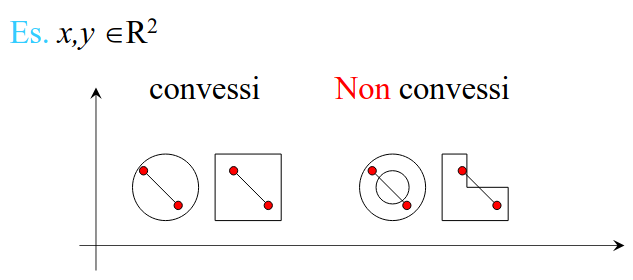
\includegraphics[width=0.75\linewidth]{image.png}
\end{figure}

\noindent\textit{Proprietà.} L'intersezione di più insiemi convessi ($F = \cap F_i$) genera sempre un insieme convesso.\\

\textit{Dimostrazione.}
\begin{align*}
    x,y\in F &\implies x,y \in F_i \hspace{0.5cm}\forall i\\
    &\implies z=\lambda x+(1-\lambda)y \in F_i \hspace{0.5cm}\forall i,\forall \lambda\\
    &\implies z\in \cap F_i
\end{align*}

\noindent\textit{Definizioni}

\begin{itemize}
    \item Un punto $z$ si definisce \textbf{vertice} di un insieme convesso $F\iff$ esso non può essere ottenuto come combinazione convessa di nessun altro punto di $F$
    \item \textbf{Chiusura convessa} ($\text{conv}(P)$): dato un insieme di punti $P$, si definisce chiusura convessa il più piccolo insieme convesso che contiene interamente $P$
\end{itemize}

\paragraph{Funzioni Convesse}
Dato un insieme convesso $F \subseteq \mathbb{R}^n$, una funzione $\varphi: F \to \mathbb{R}$ si dice convessa in $F$ se, per ogni $x, y \in F$ e $\forall \lambda \in [0,1]$, vale la disuguaglianza: 
$$ \varphi(\lambda x + (1-\lambda)y) \le \lambda \varphi(x) + (1-\lambda)\varphi(y) $$

\begin{figure}[h!]
    \centering
    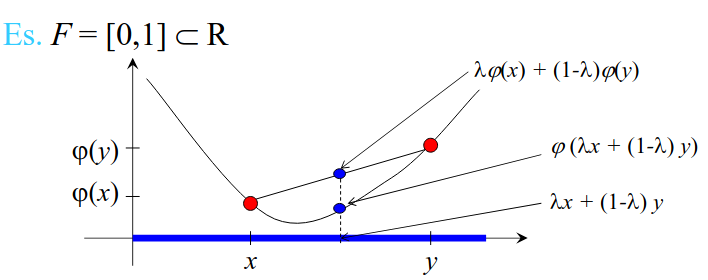
\includegraphics[width=0.75\linewidth]{convessa.png}
\end{figure}

\subsubsection{Il Problema di Ottimizzazione}
Un problema di ottimizzazione è essenzialmente una domanda formulata in termini generali, la cui risposta varia a seconda di un certo numero di parametri e variabili. Specificare dei valori concreti per i parametri genera un'\textbf{istanza} del problema.
Formalmente è descritto da:
\begin{itemize}
    \item Un vettore di \textbf{variabili decisionali} $x = (x_1, \dots, x_n) \in F'$ (dove $F'$ è l'insieme di supporto, es. $\mathbb{R}^n$).
    \item Una \textbf{regione ammissibile} $F \subseteq F'$: l'insieme di tutte le soluzioni che rispettano i vincoli. Se un punto $x \in F' \setminus F$, la soluzione non è ammissibile.
    \item Una \textbf{funzione obiettivo} (o di costo) $c: F \to \mathbb{R}$ che si intende ottimizzare.
\end{itemize}
Il problema in forma generale si indica come $$(P)\hspace{1cm}\min \{c(x) : x \in F\}$$L'obiettivo finale è trovare un $x^* \in F$ (\textbf{ottimo globale}) tale che $$z(P) = c(x^*) \le c(x)\hspace{1cm}\forall x\in F$$

\paragraph{Equivalenza min/max e Forme Matematiche}
I problemi di ottimizzazione possono essere declinati indifferentemente come minimizzazione o massimizzazione:
$$ \min \{c(x) : x \in F\} = -\max \{-c(x) : x \in F\} $$
Questi due problemi condividono esattamente lo stesso insieme di soluzioni ottime.

\noindent La regione ammissibile $F$ può essere definita:
\begin{itemize}
    \item \textbf{esplicitamente}: specificando le proprietà di $x\in F$ (ad esempio $[0,1]^2$; $x$ intere nell'ipercubo di lato 1)
    \item \textbf{implicitamente}: servendosi di equazioni e disequazioni
\end{itemize}

\begin{figure}
    \centering
    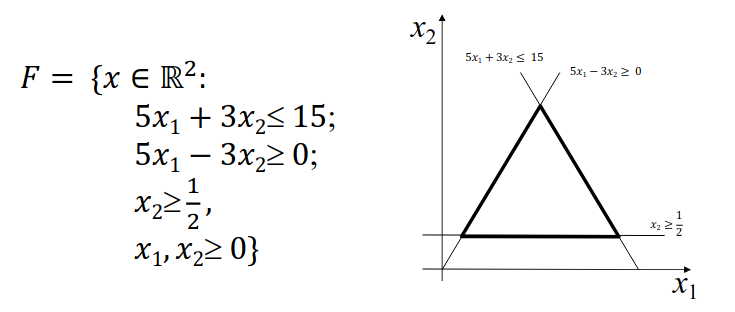
\includegraphics[width=0.75\linewidth]{regioneammissibile.png}
    \caption{Esempio di regione ammissibile definita implicitamente}
\end{figure}

\noindent Veniamo ora all'\textbf{equivalenza tra forme}. Spesso si richiede che il modello segua una struttura predefinita, convertendo le disequazioni in equazioni e viceversa. Esistono due forme notevoli:
\begin{itemize}
    \item \textbf{Forma Canonica}: $\min c^T x$ soggetta ai vincoli $Ax \ge d$, $x \ge 0$.
    \item \textbf{Forma Standard}: $\min c^T x$ soggetta ai vincoli $Ax = d$, $x \ge 0$.
\end{itemize}
Per ricondurre un modello alla forma standard:
\begin{itemize}
    \item Da un vincolo $\le$ a un'equazione: si aggiunge una \textbf{variabile slack} $x_s \ge 0$ ($x_1 + x_s = d_1$)
    \item Da un vincolo $\ge$ a un'equazione: si sottrae una \textbf{variabile surplus} $x_s \ge 0$ ($x_1 - x_s = d_1$)
\end{itemize}
Da equazioni a disequazioni:\footnote{Le trasformazioni possono aumentare i
vincoli o le variabili del modello rispetto a
quello originale.}
\[
a_i^Tx = d_i \implies \begin{cases}
    a_i^Tx \ge d_1 \\
    -a_i^Tx \ge -d_i
\end{cases}
\]

\noindent Generalmente le variabili sono vincolate in segno. Variabili di segno non vincolato (\textbf{libere}) possono essere scritte come differenza tra due variabili non negative $x_i = x_i^+ - x_i^-$ (con $x_i^+, x_i^- \ge 0$).

\subsubsection{Soluzione: i Quattro Casi Possibili}
Affrontando un problema $$(P)\hspace{0.5cm}z(P)=\min\{c(x):x\in F\}$$la regione ammissibile e la funzione di costo determinano quattro possibili scenari di soluzione:
\begin{enumerate}
    \item \textbf{Problema impossibile}: la regione ammissibile è un insieme vuoto ($F = \emptyset$) e si pone convenzionalmente $z(P) = \pm\infty$\footnote{$+\infty$ per un problema di minimo, $-\infty$ per un problema di massimo.}.
    \item \textbf{Problema illimitato (inferiormente o superiormente)}: comunque si scelga un numero reale $M$, esiste sempre una soluzione $x \in F$ tale che $c(x) \le M\textit{ }(\ge M)$. In questo caso $z(P) = -\infty\textit{ }(+\infty)$.
    \item \textbf{Valore ottimo finito, ma privo di soluzione ottima}: esiste un limite inferiore (es. $-\infty < z(P) < \infty$), ma nessun punto $x \in F$ riesce a soddisfare $c(x) = z(P)$. Questo caso è tipico di problemi strutturati male (es. ottimizzare con vincoli di tipo stretto $>$ invece che $\ge$).
    \item \textbf{Esistenza dell'ottimo globale}: il problema ha un valore ottimo finito e c'è almeno una soluzione che lo realizza.
\end{enumerate}
In fase decisionale, si affrontano anche \textbf{problemi di decisione} (verificare se esiste almeno un $x \in F$) o \textbf{problemi di certificato} (data una soluzione potenziale, verificare se essa appartiene davvero a $F$).

\subsubsection{Ottimi Locali, Globali e Tipologie di Algoritmi}
Un punto $y \in F$ si definisce \textbf{ottimo locale} se, dato un intorno euclideo $N_{\epsilon}(y) = \{x \in F : \|y - x\| \le \epsilon \}$, vale la relazione $c(y) \le c(x)$ per tutti i punti $x$ appartenenti a tale intorno.

Di norma, un algoritmo numerico iterativo cerca soluzioni esplorando intorni successivi. In un caso generico, potrebbe arrestarsi su un ottimo locale invece che raggiungere quello globale. 

\begin{figure}[h!]
    \centering
    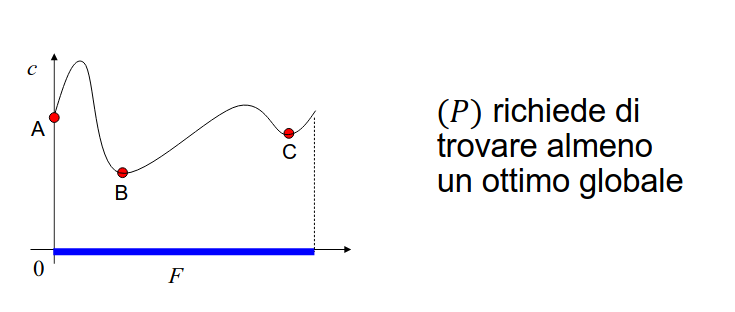
\includegraphics[width=0.5\linewidth]{mlocali.png}
\end{figure}

A questo proposito giunge in soccorso l'incredibile potenza della convessità: \textbf{se l'insieme $F$ è convesso e la funzione $c$ è anch'essa convessa, allora è dimostrato che ogni ottimo locale coincide necessariamente con un ottimo globale}.

\noindent Sotto il profilo risolutivo, esistono due macro-tipologie di algoritmi:
\begin{itemize}
    \item \textbf{Algoritmi Esatti}: garantiscono la determinazione della soluzione ottima $x^*$ (se questa esiste). Il loro svantaggio è che, per problemi di elevata complessità, possono richiedere tempi non polinomiali.
    \item \textbf{Algoritmi Euristici}: mirano a trovare una qualsiasi soluzione ammissibile in tempi accettabili, accontentandosi di un'approssimazione (inferiore o superiore) rispetto al valore ottimo reale. 
\end{itemize}
Per valutare la validità di una soluzione euristica, si calcola
\begin{itemize}
    \item l'errore assoluto $\mathcal{E}_P = |c(x) - z(P)|$; oppure
    \item l'errore relativo $\mathcal{R}_P = \frac{\mathcal{E}_P}{|z(P)|}$
\end{itemize}
\textit{Nota}: diciamo che una soluzione $x$ è $\epsilon$-approssimata se $c(x) \le \epsilon$.\\

\noindent Se $z(P)$ è del tutto incognito, spesso si aggira l'ostacolo risolvendo un \textbf{rilassamento} del problema. Un rilassamento (es. di minimo) genera un problema semplificato $\overline{P}$ tale per cui l'insieme ammissibile è espanso ($F \subseteq \overline{F}$) e la funzione di costo approssimata per difetto ($\overline{c}(x) \le c(x)$), garantendo il fatto fondamentale che $z(\overline{P}) \le z(P)$. Se la soluzione ottima $\overline{x}^*$ di $\overline{P}$ soddisfa $\overline{x}^* \in F$ e $\overline{c}(\overline{x}^*)=c(\overline{x}^*)$, allora è ottima per $P$, infatti: $$\overline{c}(\overline{x}^*) \le z(\overline{P}) \le z(P) = c(\overline{x}^*) = \overline{c}(\overline{x}^*)$$

\subsubsection{Algoritmi Numerici}
In generale, un algoritmo non possiede una visione completa e globale della regione ammissibile $F$ e della funzione obiettivo $c$. Procede invece valutando $c(x)$ in una sequenza di punti $x \in F$.

Gli algoritmi numerici per i problemi di ottimizzazione operano tipicamente in modo iterativo, seguendo questo schema generale:
\begin{enumerate}
    \item Sia $x_0 (\in F)$ una soluzione iniziale ammissibile; si pone il contatore delle iterazioni $k := 0$;
    \item \textbf{Repeat}:
    \begin{enumerate}
        \item[2.1] Verifica l'ottimalità (locale) della soluzione corrente $x_k$;
        \item[2.2] Se $x_k$ non è ottima, genera un nuovo punto ammissibile $x_{k+1} (\in F)$ tale che $c(x_{k+1}) \le c(x_k)$ e poni $k := k+1$;
    \end{enumerate}
    \item \textbf{Until}: ($x_k$ è ottima) oppure (viene soddisfatta una prefissata condizione di terminazione).
\end{enumerate}

\paragraph{Convergenza}
Applicando l'algoritmo, la sequenza di soluzioni $x_0, x_1, \dots, x_k$ converge alla soluzione ottima $x^*$ (o ad un ottimo locale). 
Nel caso generale (con $c$ ed $F$ qualsiasi), la convergenza avviene spesso verso un ottimo locale e il numero di iterazioni richiesto può essere molto elevato. 
Nel caso di problemi a variabili continue, l'algoritmo termina quando si è raggiunta l'approssimazione desiderata (tipicamente quando si registrano variazioni sufficientemente piccole tra un'iterazione e la successiva).

\paragraph{Ottimi Locali, Intorni e Convessità}
Riprendendo il concetto di ottimo locale, possiamo definire rigorosamente un \textbf{intorno euclideo} come:
$$N_\epsilon(y) = \{x \in F : \|y - x\| \le \epsilon, \epsilon > 0\}$$
Un punto $y \in F$ è un ottimo locale se $c(y) \le c(x)$ per ogni $x \in N_\epsilon(y)$. 
Un intorno $N$ si definisce \textit{esatto} se un ottimo locale rispetto ad $N$ risulta essere anche un ottimo globale (ad esempio se si potesse verificare per $N \equiv F$).

Arriviamo quindi al fondamentale teorema sulla \textbf{Convessità ed Intorno Euclideo}:\\
\textit{Dato un problema $P$ di minimo in cui la regione ammissibile $F \subseteq \mathbb{R}^n$ è convessa e la funzione obiettivo $c$ è convessa, l'intorno euclideo $N_\epsilon(y)$ è esatto per ogni $\epsilon > 0$ (quindi ogni ottimo locale coincide necessariamente con un ottimo globale).}

\noindent\textbf{Dimostrazione (per assurdo):}\\
Supponiamo che $x$ sia un ottimo locale rispetto ad un intorno $N_\epsilon(x)$, ma \textbf{non} sia l'ottimo globale. Esisterà quindi un altro punto $y \in F$ (l'ottimo globale vero) tale che $c(y) < c(x)$.

Poiché $F$ è convesso, possiamo prendere un punto $z$ come combinazione convessa di $x$ e $y$: 
$$z = \lambda x + (1-\lambda)y$$
Scegliamo un $\lambda$ sufficientemente prossimo a $1$ in modo tale che il punto $z$ cada all'interno dell'intorno $N_\epsilon(x)$.

Sfruttando la definizione di funzione convessa per $c$, sappiamo che:
$$ c(z) = c(\lambda x + (1-\lambda)y) \le \lambda c(x) + (1-\lambda)c(y) $$
Risolvendo questa disuguaglianza rispetto a $c(y)$ otteniamo:
$$ c(y) \ge \frac{c(z) - \lambda c(x)}{1-\lambda} $$
Essendo $x$ ottimo locale nell'intorno $N_\epsilon(x)$ e sapendo che $z \in N_\epsilon(x)$, vale sicuramente $c(z) \ge c(x)$. Sostituendo $c(x)$ al posto di $c(z)$ nella disuguaglianza si ottiene:
$$ c(y) \ge \frac{c(x) - \lambda c(x)}{1-\lambda} = \frac{c(x)(1-\lambda)}{1-\lambda} = c(x) $$
Siamo arrivati alla conclusione che $c(y) \ge c(x)$, il che \textbf{contraddice} palesemente la nostra ipotesi iniziale secondo cui $c(y) < c(x)$. 
Ne consegue che l'ipotesi di partenza è falsa e $x$ deve essere per forza l'ottimo globale.

\newpage

\subsection{Ottimizzazione Matematica: Modelli}

\subsubsection{Dai Problemi ai Modelli}
Una volta individuato il problema, occorre classificarlo in modo da poterlo riconoscere come appartenente a una determinata categoria, così da utilizzare algoritmi efficienti per risolverlo. La classificazione è spesso favorita descrivendo il problema tramite un \textbf{modello}, che:
\begin{itemize}
    \item Favorisce l'astrazione e la precisione.
    \item Permette di individuare similitudini tra problemi all'apparenza diversi.
\end{itemize}
In questo corso ci focalizziamo sui modelli di \textbf{Programmazione Lineare} e \textbf{Intera}.

\paragraph{Programmazione Lineare (PL e PLI)}
Un problema di Programmazione Lineare (PL o LP) è un problema di ottimizzazione definito da:
\begin{itemize}
    \item Un numero finito $n \in \mathbb{N}$ di variabili decisionali reali $x=(x_1, \dots, x_n) \in \mathbb{R}^n$.
    \item Una funzione obiettivo $f: \mathbb{R}^n \to \mathbb{R}$ lineare, nella forma $f(x) = cx$.
    \item Un insieme di $m$ vincoli lineari, nelle forme $ax = b$, $ax \le b$ o $ax \ge b$.
\end{itemize}
Talvolta è indispensabile assumere che le soluzioni ammissibili debbano essere vettori di numeri interi ($x \in \mathbb{Z}^n$): si parla in questo caso di \textbf{Programmazione Lineare Intera (PLI)}. Se solo una parte delle variabili è intera, il modello è di \textbf{Programmazione Lineare Mista (PLM)}.
Un problema di PL può sempre essere ricondotto alla forma generale $$\min \{cx \mid Ax \le b\}$$dove $A\in\mathbb{R}^{m\times n}$, $b\in\mathbb{R}^m$.

\subsubsection{Tipologie di Variabili e Vincoli Logici}
Le variabili possono essere:
\begin{itemize}
    \item \textbf{Quantitative Reali}: quantità di pezzi, proporzioni, importi economici.
    \item \textbf{Quantitative Intere}: numero di pezzi/lotti, veicoli, infrastrutture.
    \item \textbf{Logiche (Booleane $0/1$)}: esprimono decisioni binarie (attivazione/spegnimento). Vengono anche usate come variabili \textit{ausiliarie} per stabilire il verificarsi di condizioni specifiche.
    \item \textbf{A Valori Discreti}: se una variabile $x$ deve appartenere a un insieme $\{v_1, \dots, v_k\}$ di valori distinti e non continui, si introducono $k$ variabili binarie $y_i$ e si impone $\sum_{i=1}^k y_i = 1$ e $x = \sum_{i=1}^k v_i y_i$.
\end{itemize}

\paragraph{Relazioni Logiche tra Variabili}
È possibile modellare tutte le classiche relazioni logiche tramite vincoli lineari operanti su variabili booleane:
\begin{itemize}
    \item \textbf{Negazione} ($y = \text{NOT } x$): $y = 1 - x$.
    \item \textbf{Implicazione} ($x \implies y$): $y \ge x$. (Nota: se $x=1$, $y$ è forzata a $1$; se $x=0$, $y$ è libera).
    \item \textbf{Intersezione/AND} ($z = x \wedge y$): $z \le x, z \le y, z \ge x + y - 1$.
    \item \textbf{Unione/OR} ($z = x \vee y$): $z \ge x, z \ge y, z \le x + y$.
\end{itemize}
In tutti i casi $z\in\{0,1\}$. Si osservi che, se la funzione obiettivo "spinge" già la variabile ausiliaria nella direzione giusta (es. si minimizza $z$ e servono solo i vincoli che la forzano ad 1), è sufficiente imporre \textbf{metà} della relazione logica: i vincoli restanti sarebbero ridondanti.

\paragraph{Vincoli logici su variabili quantitative (big-M)}
Se $x \ge 0$ è quantitativa e $y$ binaria, la relazione "$x > 0 \implies y = 1$" (equivalentemente "$y=0 \implies x=0$") si scrive
\[
x \le M y
\]
con $M$ costante sufficientemente grande (un upper bound valido su $x$). Conviene sempre scegliere il \textbf{più piccolo} $M$ valido: valori inutilmente grandi peggiorano il rilassamento continuo e la stabilità numerica.

\subsubsection{Esempi}
\paragraph{Pianificazione della produzione} Si ha una produzione di due tipi di microprocessori (P e C). L'impianto è in grado di realizzare 3000 wafer alla settimana: su ogni wafer trovano posto 500 C oppure 300 P. La resa dipende dal processore:
\begin{itemize}
    \item resa wafer C $=60\%$ (media)
    \item resa wafer P $=50\%$ (media)
\end{itemize}
I processori P si vendono a 500€ al pezzo, i C a 200€. La divisione commerciale ha stabilito che la massima quantità di processori che possono essere messi sul mercato ogni settimana senza causare un calo dei prezzi è di 400.000 unità di P e di 700.000 unità di C. Si vuole determinare le quantità di ciascun tipo di processore da produrre settimanalmente in modo da massimizzare il ricavo totale.\\

Abbiamo un limite settimanale di 3000 wafer, dunque, considerando $w_c,w_p = $ wafer C e wafer P e considerando $x_p,x_c = $ numero di processori P e C prodotti settimanalmente:
\[
w_c + w_p \le 3000
\]
Inoltre:\footnote{Ne sopravvive solo una certa \%.}
\[
x_c = w_c\cdot 300\hspace{1cm}x_p = w_p\cdot 150
\]
Dunque
\[
\frac{x_c}{300} + \frac{x_p}{150} \le 3000 \implies \boxed{x_c + 2x_p \le 900000}
\]
Altri vincoli:
\begin{itemize}
    \item $x_p \le 400000$
    \item $x_c \le 700000$
    \item $x_p,x_c \ge 0$
\end{itemize}
È preferibile che i coefficienti siano relativamente piccoli e non troppo diversi, cioè è dato dal calcolo in notazione floating point fatto dal computer (errori di approssimazione). Possiamo esprimere $x_p$ e $x_c$ in $10^5$ pezzi e la funzione obiettivo in $10^6€$, otteniamo
\begin{itemize}
    \item $\boxed{x_c + 2x_p \le 9}$
    \item $x_p \le 4$
    \item $x_c \le 7$
    \item $x_p,x_c \ge 0$
\end{itemize}
\newpage
\noindent Dato che questo problema ha solo due variabili, possiamo disegnare la soluzione grafica:
\begin{figure}[h!]
    \centering
    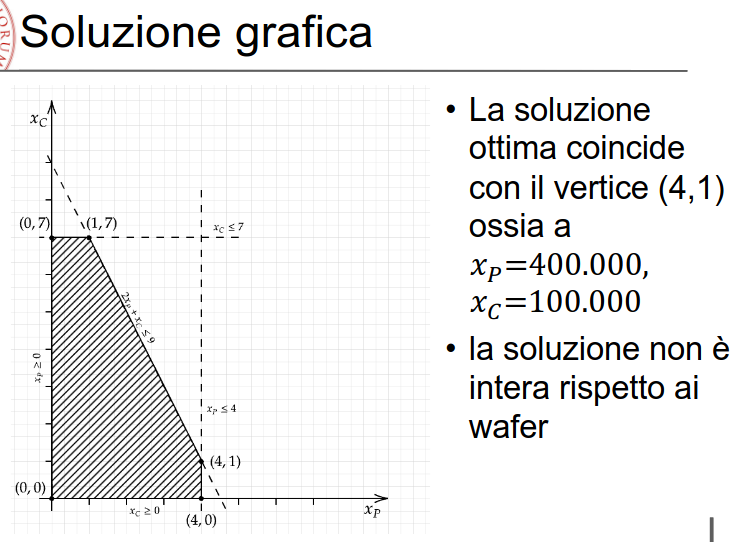
\includegraphics[width=0.75\linewidth]{processori.png}
\end{figure}

\paragraph{Fonderia} Una fonderia deve produrre 1000 pezzi del peso ciascuno di un chilogrammo. Il ferro con cui tali pezzi sono fatti dovrà contenere manganese e silicio nelle seguenti quantità:
\begin{itemize}
    \item $0.45\% \le \text{Mn}$
    \item $3.25\% \le \text{Si} \le 5.5\%$
\end{itemize}
Sono disponibili tre tipi di materiale ferroso con le seguenti caratteristiche:
\begin{table}[h!]
    \centering
    \label{fonderia}
    \begin{tabular}{lccc}
        \hline
        Materiale & A & B & C \\
        \hline
        Si (\%)        & 4.00  & 1.00  & 0.60  \\
        Mn (\%)        & 0.45  & 0.50  & 0.40  \\
        Costo (€/Kg) & 0.025 & 0.030 & 0.018 \\
        \hline
    \end{tabular}
\end{table}

\noindent Inoltre si può aggiungere Mn al costo di 10€/Kg.\\
Determinare il piano di produzione che minimizza il costo del materiale utilizzato.
\begin{itemize}
    \item Variabili decisionali: quantità di A, di B e di C + quantità di Mn puro da acquistare
    \item Vincoli: vincoli di quantità (totale $=/\ge 1000$ kg) + vincoli sulle percentuali
    \item Funzione obiettivo: costo sulla miscela
\end{itemize}
Calcoliamo i vincoli percentuali. Ricordiamo $0.45\% \le \textit{Mn}$. Dunque, considerando la tabella \ref{fonderia} e considerando che $x_A,x_B,x_C,x_M = $ kg di $A,B,C,\textit{Mn}$ da acquistare:
\[
0.45x_A + 0.50x_B + 0.40x_C + 100x_M \ge \underbrace{450}_{0.45\cdot 1000}
\]
Passiamo ora ai vincoli sul silicio. Il primo è $\textit{Si} \ge 3.25\%$. Considerando sempre la tabella \ref{fonderia}:
\[
4.00x_A + 1.00x_B + 0.60x_C \ge 3250
\]
E l'altro è $\textit{Si} \le 5.5\%$, dunque:
\[
4.00x_A + 1.00x_B + 0.60x_C \le 5500
\]
Tutti i vincoli:
\begin{itemize}
    \item $x_A + x_B+x_C + x_M \ge 1000$ kg\footnote{La consegna richiede che sia uguale, ma in questo caso può essere conveniente da un punto di vista di calcoli richiedere che sia maggiore o uguale.}
    \item $x_A,x_B,x_C,x_M \ge 0$
    \item $0.45x_A + 0.50x_B + 0.40x_C + 100x_M \ge 450$
    \item $4.00x_A + 1.00x_B + 0.60x_C \ge 3250$
    \item $4.00x_A + 1.00x_B + 0.60x_C \le 5500$
\end{itemize}
Ricordiamo, vogliamo minimizzare la funzione obiettivo del costo totale (vedi tabella \ref{fonderia}):
\[
Z = 0.025x_A + 0.030x_B + 0.018x_C + 10x_M
\]

\paragraph{Problema della dieta} Si hanno $n$ alimenti e $m$ sostanze nutritive. Inoltre:
\begin{itemize}
    \item $a_{ij} = $ quantità della sostanza $i$ in un'unità dell'alimento $j$ ($i=1..m; j=1..n$)
    \item $d_i = $ fabbisogno della sostanza $i$ ($i=1..m$)
    \item $c_j = $ costo dell'unità dell'alimento $j$ ($j=1..n$)
\end{itemize}
Determinare il mix di alimenti di minimo costo che garantisce il fabbisogno delle sostanze nutritive. Vogliamo cioè, con $x_j = $ q.tà alimento $j$ da acquistare ($j=1..m$):
\[
\min c(x) = \sum_{j=1}^n c_jx_j
\]
Requisiti:
\begin{itemize}
    \item $x_j \ge 0$
    \item $\sum_{j=1}^n a_{ij}x_j \ge d_i$
\end{itemize}

\newpage

\paragraph{Problema dello zaino (KP)} Dato un contenitore (zaino) di capacità $b$ e un insieme $E=\{1..n\}$ di $n$ oggetti, ciascuno caratterizzato da:
\begin{itemize}
    \item peso $a_i$
    \item profitto $c_i$
\end{itemize}
Determinare il sottoinsieme $S \subseteq E$ di oggetti di profitto massimo il cui peso complessivo non superi la capacità. Dunque, devo determinare $S\subseteq E$ tale che:
\[
F = \left\{S \subseteq E:\sum_{i\in S} a_i \le b \right\}
\]
\[
c(S) = \sum_{i\in S} c_i
\]
Le soluzioni possibili sono tutti i sottoinsiemi di $E$ che sono $2^{|E|} = 2^n$. La soluzione ottima è
\[
S^* = \min\{c(S):S\in F\}
\]
È un tipico problema di \textbf{selezione}:
\[
\forall i=1..n \hspace{1cm} x_i = \begin{cases}
    1 & \text{se }i\in S^*\\
    0 & \mathrm{altrimenti}
\end{cases}
\]
Funzione obiettivo:
\[
\max c(x) = \sum_{i=1}^n c_ix_i
\]
Vincolo:
\[
\sum_{i=1}^n a_ix_i \le b, \hspace{1cm} x_i\in\{0,1\}, i=1..n
\]

\noindent\textit{Esempio numerico.} Sia $n=5$, $b=10$, $c=(12,12,7,6,2)$, $a=(4,5,3,3,2)$. La soluzione $x=(1,1,0,0,0)$ è ammissibile e vale $c(x)=24$ (è un \textbf{lower bound}, essendo un problema di massimo). Un \textbf{upper bound} si ottiene risolvendo il rilassamento continuo con la regola greedy: si ordinano gli oggetti per rapporto $c_i/a_i$ decrescente e li si inserisce finché entrano, prendendo una \textit{frazione} del primo che non ci sta:
\[
U = \left\lfloor 12 + 12 + \tfrac{1}{3}\cdot 7 \right\rfloor = 26
\]
La soluzione ottima è $x^*=(1,0,1,1,0)$ con $c(x^*)=25$: si noti che $24 \le 25 \le 26$, cioè l'ottimo è sempre compreso tra il valore di una qualsiasi soluzione ammissibile e il valore del rilassamento.

\paragraph{Min-cost Spanning Tree (MST)} Dato un grafo non orientato $G=(N,A)$
\begin{itemize}
    \item $N$ insieme dei nodi (vertici) con $|N|=n$
    \item $A$ insieme degli archi con $|A|=m$
    \item $\forall a\in A,c_a\ge 0$ costo dell'arco
\end{itemize}
Determinare un grafo parziale $G'=(N,A')$ connesso e aciclico di costo minimo
\[
F = \left\{ T\subseteq A:(N,T)\text{ è uno spanning tree di G} \right\}
\]
\[
c(T) = \sum_{a\in A} c_a
\]
La soluzione ottima è $T^*=\min\{c(T):T\in F\}$. $T^*$ contiene un sottoinsieme di archi del grafo $\implies$ problema di selezione:
\[
\forall a\in A,\hspace{1cm}x_a=\begin{cases}
    1 & \text{se }a\in T^*\\
    0&\mathrm{altrimenti}
\end{cases}
\]
\newpage
\noindent Affinché $T$ sia connesso ogni taglio $(N',N'')$ di $G$ dev'essere attraversato da un arco in $T$
\begin{figure}[h!]
    \centering
    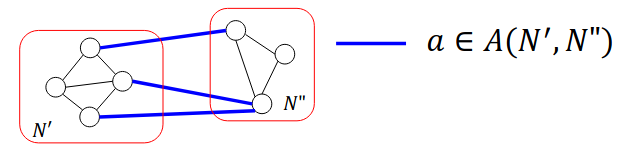
\includegraphics[width=0.65\linewidth]{mst1.png}
\end{figure}

\begin{figure}[h!]
    \centering
    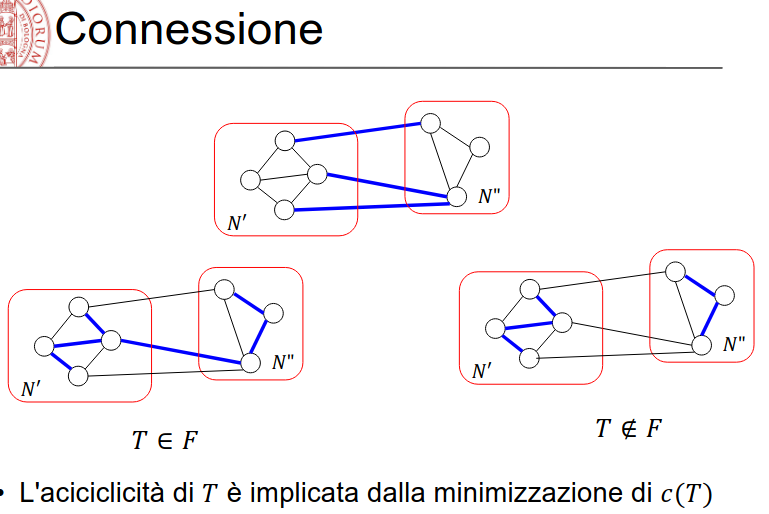
\includegraphics[width=0.5\linewidth]{connessione.png}
\end{figure}

\noindent Dunque:
\[
\forall a\in A,\hspace{1cm}x_a=\begin{cases}
    1 & \text{se }a\in T^*\\
    0&\mathrm{altrimenti}
\end{cases}
\]
\[
\min c(x) = \sum_{a\in A} = c_ax_a
\]
Vincoli:
\[
\sum_{a\in A(N',N'')} x_a \ge 1\hspace{1cm}\forall(N',N''),x_a\in\{0,1\},a\in A
\]
La formulazione ha un numero esponenziale di vincoli!

\paragraph{Problema del commesso viaggiatore (TSP)}
Un commesso viaggiatore deve visitare $n$ città in modo tale che il viaggio abbia lunghezza minima. 
Dato un grafo orientato completo $G=(N,A)$:
\begin{itemize}
    \item $N$ è l'insieme dei nodi (città) con $|N|=n$.
    \item $A$ è l'insieme degli archi con $|A|=m$.
    \item $\forall (i,j) \in A, c_{ij} \ge 0$ è il costo dell'arco.
\end{itemize}

L'obiettivo è determinare un grafo parziale $G'=(N,A')$ che sia un ciclo Hamiltoniano di costo minimo, ovvero un ciclo che visiti ciascun nodo una sola volta.
\[
F = \{P\subseteq A:(N,P)\text{ è ciclo hamiltoniano di }G\}
\]
\[
c(P) = \sum_{(i,j)\in P} c_{ij}
\]
Il problema è modellato come un problema di selezione utilizzando variabili decisionali binarie:
\[
x_{ij} = \begin{cases} 
1 & \text{se } (i,j) \in P^* \\ 
0 & \text{altrimenti} 
\end{cases} \quad \forall (i,j) \in A
\]

\noindent Il modello matematico completo è definito come segue:
\[
\min c(x) = \sum_{(i,j) \in A} c_{ij}x_{ij}
\]

\noindent Soggetto ai vincoli:
\begin{itemize}
    \item \textbf{Vincoli di grado}: Ogni nodo deve avere esattamente due archi incidenti (uno in entrata e uno in uscita) per garantire la visita singola:
    \[ \sum_{j:(i,j) \in A} x_{ij} = 2 \quad i=1, \dots, n \]
    \item \textbf{Vincoli di connessione}: Per evitare la formazione di sotto-cicli isolati (sub-tours), è necessario imporre la connessione tramite vincoli sui tagli, analogamente al modello MST:
    \[ \sum_{(i,j) \in A(N', N'')} x_{ij} \ge 1 \quad \forall (N', N'') \]
\end{itemize}

Questa formulazione presenta un numero esponenziale di vincoli. Si osserva che il modello TSP include la struttura del MST con l'aggiunta dei vincoli di grado; pertanto, il problema MST costituisce un rilassamento del TSP. Esistono inoltre formulazioni alternative che utilizzano un numero polinomiale di vincoli.

\subsubsection{Assegnamento}

\paragraph{Vincoli di assegnamento}
Spesso si ha la necessità di modellare associazioni tra entità del problema. Un esempio tipico è l'assegnazione di oggetti a luoghi. Dato un insieme $N = \{1,\ldots,n\}$ di oggetti e un insieme $V = \{1,\ldots,m\}$ di luoghi, si introducono variabili binarie per rappresentare le assegnazioni:

\[
\forall(i,j), \quad x_{ij} = \begin{cases} 
1 & \text{se oggetto } i \text{ assegnato a luogo } j \\ 
0 & \text{altrimenti}
\end{cases}
\]

\noindent A seconda delle caratteristiche del problema, si possono definire diverse tipologie di vincoli di assegnamento. Nel caso del \textit{semi-assegnamento}, ogni oggetto può essere assegnato ad un solo luogo, il che si traduce nel vincolo:

\[
\sum_{j=1}^{m} x_{ij} = 1 \quad i = 1, \dots, n
\]

In alcuni contesti, non tutti i luoghi sono ammissibili per un determinato oggetto. Se $B_i \subseteq V$ rappresenta l'insieme dei luoghi ammissibili per l'oggetto $i$, il vincolo diventa:

\[
\sum_{j \in B_i} x_{ij} = 1 \quad i = 1, \dots, n
\]

Nel caso dell'\textit{assegnamento completo}, si richiede che ogni oggetto sia assegnato ad un solo luogo e che ogni luogo riceva esattamente un oggetto. Nel caso $m = n$, si ha:

\[
\sum_{j=1}^{m} x_{ij} = 1 \quad i = 1, \dots, n \qquad \sum_{i=1}^{n} x_{ij} = 1 \quad j = 1, \dots, m
\]

Se il numero di luoghi è maggiore del numero di oggetti ($m > n$), alcuni luoghi possono rimanere inutilizzati:

\[
\sum_{j=1}^{m} x_{ij} = 1 \quad i = 1, \dots, n \qquad \sum_{i=1}^{n} x_{ij} \leq 1 \quad j = 1, \dots, m
\]

Viceversa, se il numero di oggetti è maggiore del numero di luoghi ($m < n$), alcuni oggetti potrebbero rimanere non assegnati:

\[
\sum_{j=1}^{m} x_{ij} \leq 1 \quad i = 1, \dots, n \qquad \sum_{i=1}^{n} x_{ij} = 1 \quad j = 1, \dots, m
\]

\paragraph{Problema dell'assegnamento}
Un'applicazione classica dei vincoli di assegnamento è il problema dell'assegnazione di incarichi a persone. Dato un insieme $N = \{1,\ldots,n\}$ di persone e un insieme $V = \{1,\ldots,n\}$ di incarichi (tipicamente con $m = n$), per ogni coppia persona-incarico $(i,j)$ è definito un costo $c_{ij}$ che rappresenta, ad esempio, il tempo di esecuzione o il costo dell'assegnamento (se l'assegnamento non è possibile, si pone $c_{ij} = +\infty$). L'obiettivo è determinare l'assegnamento di costo complessivo minimo.

Utilizzando le stesse variabili binarie $x_{ij}$ definite in precedenza, il problema dell'assegnamento (Assignment Problem, AP) si formula come:

\[
\begin{aligned}
\min c(x) &= \sum_{i=1}^{n} \sum_{j=1}^{n} c_{ij} x_{ij} \\
\text{(AP)} \quad \sum_{j=1}^{n} x_{ij} &= 1 \quad i = 1, \dots, n \\
\sum_{i=1}^{n} x_{ij} &= 1 \quad j = 1, \dots, n \\
x_{ij} &\in \{0,1\} \quad i, j = 1, \dots, n
\end{aligned}
\]

I vincoli garantiscono che ogni persona riceva esattamente un incarico e che ogni incarico sia assegnato ad una sola persona, realizzando così una corrispondenza biunivoca tra persone e incarichi.

\paragraph{Ordinamento di lavori su macchine - Min Cardinality Machine Scheduling}
\begin{itemize}
    \item Dati $n$ lavori, ciascun lavoro $i = 1, \ldots, n$:
    \begin{itemize}
        \item disponibile dall'istante $t_i$ (la lavorazione deve iniziare immediatamente)
        \item supponiamo $t_1 \leq t_2 \leq \ldots \leq t_n$
        \item richiede di essere lavorato per $d_i$ istanti,
        \item termina a $t_i + d_i$
    \end{itemize}
    \item $m$ macchine identiche ($m \leq n$)
    \item Assegnare i lavori alle macchine senza sovrapposizione e minimizzando il numero di macchine usate
\end{itemize}
La soluzione consiste in una partizione dei lavori in insiemi $N(1), \ldots, N(m)$ eventualmente vuoti in cui $N(j)$ è l'insieme dei lavori sulla macchina $j$.

\[
\forall(i,j), \quad x_{ij} = \begin{cases}
1 & \text{se lavoro } i \text{ assegnato a macchina } j \\
0 & \text{altrimenti}
\end{cases}
\quad i = 1, \dots, n; \; j = 1, \dots, m
\]

\noindent Ogni lavoro deve essere eseguito su una macchina:

\[
\sum_{j=1}^{m} x_{ij} = 1 \quad i = 1, \dots, n
\]
Due lavori possono essere lavorati sulla stessa macchina se gli intervalli di lavorazione sono disgiunti:

\[
\forall h,k \quad t_h \geq t_k + d_k \quad \text{oppure} \quad t_k \geq t_h + d_h
\]

\noindent Se gli intervalli di lavorazione sono sovrapposti, due lavori non possono essere eseguiti sulla stessa macchina. Sia $S(i) =$ lavori incompatibili con $i$ per $i = 1, \ldots, n-1$:

\[
S(i) = \{h = i+1, \ldots, n: [t_i, t_i+d_i] \cap [t_h, t_h+d_h] \neq \emptyset\}
\]

\noindent Vincoli di compatibilità:

\[
x_{ij} + x_{hj} \leq 1 \quad i = 1, \dots, n-1; \; h \in S(i); \; j = 1, \dots, m
\]
Per "contare" le macchine usate abbiamo bisogno di variabili che ne indichino l'uso:

\[
\forall j = 1, \ldots, m, \quad y_j = \begin{cases}
1 & \text{se la macchina } j \text{ è utilizzata} \\
0 & \text{altrimenti}
\end{cases}
\]

\noindent Il modello completo del problema di minimizzazione del numero di macchine utilizzate è:

\[
\begin{aligned}
\min c(y) &= \sum_{j=1}^{m} y_j \\
\sum_{j=1}^{m} x_{ij} &= 1 \quad i = 1, \dots, n \\
x_{ij} + x_{hj} &\leq 1 \quad i = 1, \dots, n-1; \; h \in S(i); \; j = 1, \dots, m \\
x_{ij} &\leq y_j \quad i = 1, \dots, n; \; j = 1, \dots, m \\
x_{ij} &\in \{0,1\} \quad i = 1, \dots, n; \; j = 1, \dots, m \\
y_j &\in \{0,1\} \quad j = 1, \dots, m
\end{aligned}
\]

\noindent I vincoli hanno il seguente significato:
\begin{itemize}
    \item I primi vincoli garantiscono che ogni lavoro sia assegnato ad esattamente una macchina.
    \item I vincoli di compatibilità assicurano che due lavori incompatibili (con intervalli temporali sovrapposti) non vengano assegnati alla stessa macchina.
    \item I vincoli $x_{ij} \leq y_j$ impongono che se un lavoro è assegnato alla macchina $j$, allora la macchina $j$ deve essere considerata utilizzata ($y_j = 1$).
    \item La funzione obiettivo minimizza il numero totale di macchine utilizzate.
\end{itemize}

\noindent\textit{Osservazione (aggregazione dei vincoli).} Gli $nm$ vincoli di legame $x_{ij}\le y_j$ possono essere sostituiti dagli $m$ vincoli aggregati
\[
\sum_{i=1}^n x_{ij} \le n\, y_j \quad j=1,\dots,m
\]
che esprimono la stessa implicazione ma con molti meno vincoli. Attenzione al trade-off: la formulazione aggregata è più compatta ma il suo rilassamento continuo è \textbf{più debole} (permette $y_j$ frazionarie molto piccole), quindi tipicamente più lenta da risolvere con Branch-and-Bound.

\subsubsection{Selezione di Sottoinsiemi}
Sia $N=\{1,\dots,n\}$ un insieme finito di elementi e sia $F=\{F_1,\dots,F_m\}$ una famiglia di suoi sottoinsiemi, dove $F_j \subseteq N$.
Ogni sottoinsieme $F_j$, per $j=1,\dots,m$, ha un costo associato $c_j > 0$.
L'obiettivo è determinare una collezione di sottoinsiemi $D \subseteq F$ di costo minimo che soddisfi determinati vincoli specifici. Un generico sottoinsieme $F_j$ può essere descritto tramite un vettore di incidenza (o matrice) $A$, dove l'elemento $a_{ij}$ è definito come:
\[
a_{ij} = \begin{cases}
1 & \text{se } i \in F_j \\
0 & \text{altrimenti}
\end{cases}
\]
dove $i$ è un singolo elemento di $N$.
Per modellare la scelta, introduciamo delle variabili decisionali logiche:
\[
x_j = \begin{cases}
1 & \text{se } j \in D \text{ (il sottoinsieme } F_j \text{ è selezionato)} \\
0 & \text{altrimenti}
\end{cases} \quad j=1,\dots,m
\]
La funzione obiettivo, che minimizza il costo totale, sarà dunque:
\[
\min c(x) = \sum_{j=1}^m c_j x_j
\]
A seconda dei vincoli applicati su come questi sottoinsiemi devono coprire l'insieme $N$, otteniamo tre problemi classici.

\paragraph{Set Covering Problem (SCP)}
Nel problema di copertura (Set Covering), si richiede che ogni elemento $i \in N$ sia contenuto in \textbf{almeno un} sottoinsieme selezionato in $D$.
Il modello matematico è:
\[
\begin{aligned}
\text{(SCP)} \quad \min c(x) &= \sum_{j=1}^m c_j x_j \\
\sum_{j=1}^m a_{ij}x_j &\ge 1 \quad i=1,\dots,n \\
x_j &\in \{0,1\} \quad j=1,\dots,m
\end{aligned}
\]

\paragraph{Set Partitioning Problem (SPP)}
Nel problema di partizionamento (Set Partitioning), la condizione è più stringente: ogni elemento $i \in N$ deve essere contenuto in \textbf{esattamente un} sottoinsieme selezionato in $D$.
Il modello matematico diventa:
\[
\begin{aligned}
\text{(SPP)} \quad \min c(x) &= \sum_{j=1}^m c_j x_j \\
\sum_{j=1}^m a_{ij}x_j &= 1 \quad i=1,\dots,n \\
x_j &\in \{0,1\} \quad j=1,\dots,m
\end{aligned}
\]

\paragraph{Set Packing Problem (SPkP)}
Nel problema di riempimento (Set Packing), la condizione è che ogni elemento $i \in N$ deve essere contenuto in \textbf{al più un} sottoinsieme selezionato in $D$. Generalmente, questo problema è formulato come un problema di massimizzazione del profitto, altrimenti la soluzione ottima banale in un problema di minimo con soli costi positivi sarebbe non prendere nulla ($D = \emptyset$).
\[
\begin{aligned}
\text{(SPkP)} \quad \max c(x) &= \sum_{j=1}^m c_j x_j \\
\sum_{j=1}^m a_{ij}x_j &\le 1 \quad i=1,\dots,n \\
x_j &\in \{0,1\} \quad j=1,\dots,m
\end{aligned}
\]

\subsubsection{Localizzazione Infrastrutture}

\paragraph{Apertura Centri CUP}
Un'applicazione classica del Set Covering è la localizzazione di infrastrutture. Supponiamo di voler aprire dei centri CUP in una città divisa in 6 zone (massimo 1 sito per quartiere). Vogliamo minimizzare il numero di centri aperti, garantendo che il tempo massimo di trasferimento da qualsiasi quartiere al centro CUP più vicino sia al massimo di 15 minuti.
A partire da una matrice delle distanze temporali, costruiamo una matrice logica di vicinanza: $a_{ij} = 1$ se dalla zona $i$ si può raggiungere la zona $j$ in $\le 15$ minuti, e $0$ altrimenti. Definiamo le variabili:
\[
x_i = \begin{cases}
1 & \text{se si attiva il CUP nella zona } i \\
0 & \text{altrimenti}
\end{cases} \quad i=1,\dots,6
\]

\begin{figure}[h!]
    \centering
    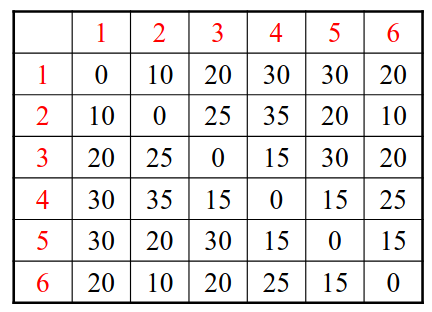
\includegraphics[width=0.35\linewidth]{cup.png}
    \caption{Tempi di trasferimento tra quartieri}
\end{figure}

\clearpage

\begin{figure}[h!]
    \centering
    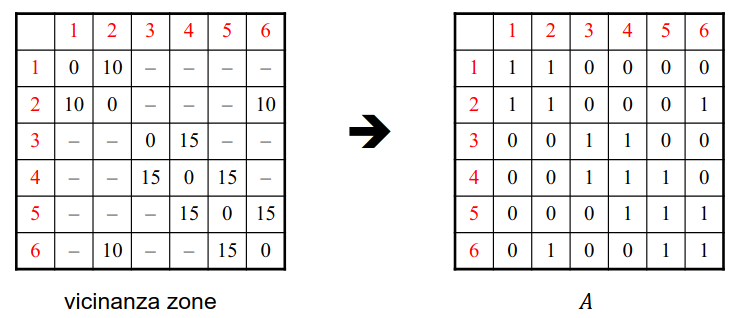
\includegraphics[width=0.5\linewidth]{cup2.png}
\end{figure}

\noindent Il modello (PLI) per minimizzare il numero di centri aperti sarà:
\[
\min \sum_{i=1}^6 x_i
\]
Soggetto ai vincoli di copertura (ricavati leggendo le righe della matrice di adiacenza delle zone a distanza $\le 15$):
\begin{align*}
1:&\quad x_1 + x_2 \ge 1 \\
2:&\quad x_1 + x_2 + x_3 + x_4 + x_6 \ge 1 \\
3:&\quad x_3 + x_4 \ge 1 \\
4:&\quad x_3 + x_4 + x_5 \ge 1 \\
5:&\quad x_4 + x_5 + x_6 \ge 1 \\
6:&\quad x_2 + x_5 + x_6 \ge 1 \\
&\quad x_1, \dots, x_6 \in \{0,1\}
\end{align*}

\paragraph{Localizzazione di Infrastrutture Nocive (Obnoxious Facility Location)}
Supponiamo che una regione debba localizzare dei termovalorizzatori. Sono stati individuati $m$ siti possibili vicino a $n$ città principali. 
Per ogni sito $j=1,\dots,m$ sono noti:
\begin{itemize}
    \item $b_j$: costo di costruzione (in milioni di euro).
    \item $c_j$: capacità di trattamento (in migliaia di tonnellate).
\end{itemize}
Inoltre, consideriamo una matrice di prossimità dove $a_{ij}=1$ se la città $i$ è "vicina" al sito $j$, e $0$ altrimenti.
Le regole sono:
\begin{itemize}
    \item Budget totale disponibile: $B$.
    \item Ogni città non può avere \textbf{più di un} sito attivo "vicino".
    \item Obiettivo: massimizzare la capacità totale dei siti attivati.
\end{itemize}

Utilizzando variabili binarie $x_j = 1$ se il sito $j$ è attivato e $0$ altrimenti, il modello si formula così:
\[
\begin{aligned}
\text{(P)} \quad \max c(x) &= \sum_{j=1}^m c_j x_j \\
\text{Vincolo di prossimità:} \quad \sum_{j=1}^m a_{ij}x_j &\le 1 \quad i=1,\dots,n \\
\text{Vincolo di budget:} \quad \sum_{j=1}^m b_j x_j &\le B \\
x_j &\in \{0,1\} \quad j=1,\dots,m
\end{aligned}
\]

\subsubsection{Variabili a Valori Discreti (Richiamo)}
Come già accennato in precedenza, capita spesso che le variabili siano vincolate ad assumere valori in un insieme finito e discreto di numeri reali distinti che non sono necessariamente un intervallo continuo o un semplice insieme $\{0,1\}$. Ad esempio, poniamo che $x$ debba appartenere all'insieme $\{v_1, \dots, v_k\}$.
Per modellare questo comportamento linearmente, si introducono $k$ variabili binarie $y_i \in \{0,1\}$ per $i=1,\dots,k$, e si impone che esattamente una di esse sia pari a 1:
\[
\sum_{i=1}^k y_i = 1
\]
Il valore della variabile originale $x$ sarà quindi dato dalla combinazione lineare di questi valori pesati per le variabili booleane:
\[
x = \sum_{i=1}^k v_i y_i
\]

\subsubsection{Progetto di Reti (Network Design)}
Consideriamo ora il problema di dover definire una rete fognaria per collegare alcuni centri abitati ad un depuratore centrale. 
Dati del problema:
\begin{itemize}
    \item Un grafo orientato $G=(V,A)$ dove $V$ sono i nodi (i centri abitati e il depuratore) e $A$ sono gli archi (i possibili collegamenti idraulici).
    \item Ogni centro $i$ produce una quantità di liquidi $b_i$.
\end{itemize}

Per formulare il problema, introduciamo per ogni arco $(i,j) \in A$ una variabile quantitativa continua:
\[
x_{ij} = \text{flusso di rifiuti sull'arco } (i,j) \text{ (con } x_{ij} \ge 0 \text{, e } x_{ij}=0 \text{ se l'arco non è usato)}
\]

\paragraph{Bilanciamento del flusso}
Il principio cardine dell'ottimizzazione su reti è il \textbf{bilanciamento del flusso}. Per ogni nodo della rete, il flusso portato dagli archi \textit{uscenti} deve essere uguale al flusso portato dagli archi \textit{entranti} più la quantità \textit{prodotta} (o domandata) localmente nel nodo.

\newpage

\noindent Matematicamente, per un generico nodo $i$, si esprime in questo modo:
\[
\underbrace{\sum_{l: (l,i) \in A} x_{li}}_\text{ciò che entra} - \underbrace{\sum_{j: (i,j) \in A} x_{ij}}_\text{ciò che esce} = b_i
\]
dove
\begin{itemize}
    \item $b_i \ge 0$ se il nodo è un \textbf{pozzo} (domanda) o di \textbf{transito}
    \item $b_i < 0$ se il nodo è una \textbf{sorgente} (produzione)
\end{itemize}

\begin{figure}[h!]
    \centering
    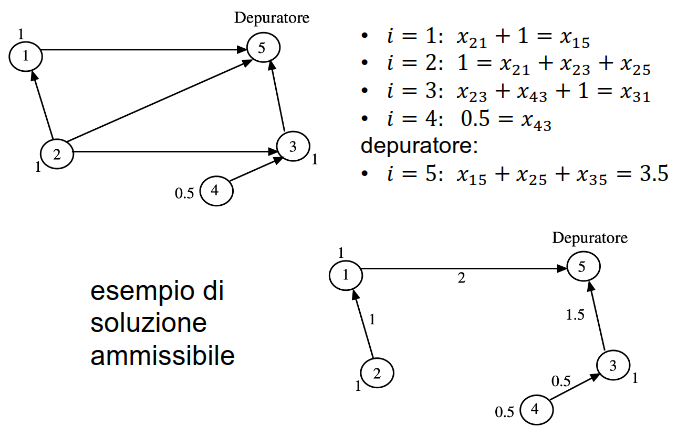
\includegraphics[width=0.5\linewidth]{bil_flusso.png}
\end{figure}

\paragraph{Funzione obiettivo e Capacità}
Su ogni arco $(i,j)$ utilizzato, deve essere installata una condotta la cui portata sia almeno pari al flusso $x_{ij}$ che lo attraversa. In genere, il costo di posa non è una semplice funzione lineare ma presenta economie di scala a gradini, poiché le condotte in commercio sono disponibili solo per un sottoinsieme discreto di portate (es. $p_h \in \{0.0,0.7, 1.4, 3.0\}$ con costi associati $c_h$).
Omettendo la portata zero, consideriamo $k$ tipi di condotte standard. Introduciamo le variabili binarie:
\[
y_{ij}^h = \begin{cases}
1 & \text{se sull'arco } (i,j) \text{ viene installata la condotta di portata } p_h \\
0 & \text{altrimenti}
\end{cases}
\]

\noindent Il nostro scopo è minimizzare il costo di installazione, assicurando la compatibilità dimensionale tra i flussi transitanti e i tubi scelti:
\[
\text{Compatibilità flusso-portata:} \quad x_{ij} \le \sum_{h=1}^k p_h y_{ij}^h \quad \forall (i,j) \in A
\]
Inoltre, su ogni arco si può installare al massimo una tipologia di tubo:
\[
\sum_{h=1}^k y_{ij}^h \le 1 \quad \forall (i,j) \in A
\]

\paragraph{Modello Completo}
Raccogliendo tutti gli elementi (con $n$ nodi totali e $k$ tipi di condotte disponibili), il modello intero misto assume questa veste finale:
\[
\begin{aligned}
\min \quad & \sum_{(i,j) \in A} \sum_{h=1}^k c_h y_{ij}^h \\
\text{s.t.} \quad & \sum_{l: (l,i) \in A} x_{li} - \sum_{j: (i,j) \in A} x_{ij} = b_i \quad i=1,\dots,n \\
& x_{ij} \le \sum_{h=1}^k p_h y_{ij}^h \quad \forall (i,j) \in A \\
& \sum_{h=1}^k y_{ij}^h \le 1 \quad \forall (i,j) \in A \\
& x_{ij} \ge 0 \quad \forall (i,j) \in A \\
& y_{ij}^h \in \{0,1\} \quad \forall (i,j) \in A, \: h=1,\dots,k
\end{aligned}
\]

\subsubsection{Minima quantità positiva}
Quando una variabile $x$ rappresenta un certo livello di produzione, capita spesso che il valore di tale variabile debba appartenere a un insieme del tipo $\{0\} \cup [l, u]$.
Questo significa che:
\begin{itemize}
    \item $0$ rappresenta l'assenza di produzione;
    \item l'intervallo $[l, u]$ rappresenta i possibili livelli di produzione quando questa effettivamente avviene (quindi non si può produrre meno di una quantità minima $l$).
\end{itemize}
Per modellare questa situazione, introduciamo una variabile logica ausiliaria $y \in \{0,1\}$ che indica la presenza ($y=1$) o meno ($y=0$) di produzione.
I vincoli lineari che legano $x$ a $y$ sono:
\[
l y \le x \le u y
\]
In questo modo, se $y=0$, allora $0 \le x \le 0 \implies x=0$. Altrimenti, se $y=1$, avremo $l \le x \le u$.

\subsubsection{Costo fisso di produzione (Carico Fisso)}
Collegato al concetto precedente è il problema del mix di produzione con costo fisso. Se decidiamo di produrre un bene $j$, dobbiamo sostenere un costo (o carico) fisso $F_j$ (ad esempio, per accendere i macchinari), a cui si somma il costo di produzione variabile dipendente dalla quantità $x_j$, indicato con $p_j$.
Il contributo del prodotto $j$ alla funzione obiettivo è quindi:
\[
\text{Costo}_j = \begin{cases}
0 & \text{se non prodotto } (x_j = 0) \\
F_j + p_j x_j & \text{se prodotto } (x_j > 0)
\end{cases}
\]

\newpage

\begin{figure}[h!]
    \centering
    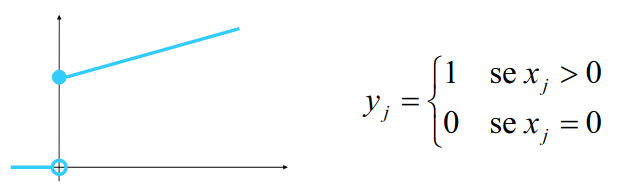
\includegraphics[width=0.75\linewidth]{costofissoprod.png}
\end{figure}

Questo genera una discontinuità nell'origine.
Per modellare la funzione obiettivo linearmente, usiamo ancora una volta variabili binarie:
\[
y_j = \begin{cases}
1 & \text{se } x_j > 0 \\
0 & \text{se } x_j = 0
\end{cases}
\]
La funzione obiettivo diventa:
\[
\min \sum_{j=1}^n (F_j y_j + p_j x_j)
\]
Occorre legare tra loro le variabili decisionali quantitative $x_j$ e quelle logiche $y_j$ con vincoli lineari noti come vincoli logici ("big-M"):
\[
x_j \le M y_j \quad j=1,\dots,n
\]
dove $M$ è una costante molto grande (teoricamente vicina a $+\infty$, praticamente un upper bound del valore di $x_j$).
\begin{itemize}
    \item Se $y_j = 0$, allora $x_j \le 0$, ma siccome in genere $x_j \ge 0$, si forza $x_j = 0$.
    \item Se $y_j = 1$, allora $x_j \le M$, lasciando la variabile $x_j$ libera di assumere il suo valore.
\end{itemize}
Non è necessario imporre anche l'altra "metà" della relazione logica (ovvero forzare $y_j=0$ se $x_j=0$), perché essendo un problema di minimizzazione, l'algoritmo eviterà autonomamente di porre $y_j=1$ se $x_j=0$, per non pagare inutilmente il costo fisso $F_j$. Le variabili $y_j$ in questo caso fungono da vere e proprie \textbf{variabili ausiliarie}.

\begin{figure}[h!]
    \centering
    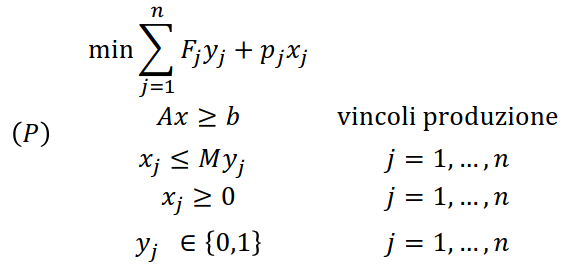
\includegraphics[width=0.75\linewidth]{costofissodiprod2.png}
\end{figure}

\subsubsection{Vincoli di soglia}
Date $n$ variabili $\{x_1, \dots, x_n\}$, può essere necessario definire dei valori soglia mediante vincoli lineari.
Se vogliamo definire un limite inferiore $l$ come il minimo tra le variabili ($l \le \min\{x_1, \dots, x_n\}$) o un limite superiore $u$ come il massimo ($u \ge \max\{x_1, \dots, x_n\}$), possiamo usare $n$ vincoli lineari separati:
\[
l \le x_i \quad \text{oppure} \quad u \ge x_i \quad \forall i=1,\dots,n
\]
Se nella funzione obiettivo si massimizza $l$ (o si minimizza $u$), il valore ottimo coinciderà esattamente con il minimo (o massimo) reale dell'insieme $\{x_1, \dots, x_n\}$.

\subsubsection{Ordinamento di lavori su macchine: Min Makespan Machine Scheduling}
Questa è una variante del problema MCMS (Min Cardinality Machine Scheduling) visto in precedenza. Qui abbiamo un numero fisso di macchine $m$ e $n$ lavori. Ogni lavoro richiede un tempo di esecuzione (processing time) $d_i$. Vogliamo assegnare i lavori alle macchine senza sovrapposizione per minimizzare il tempo massimo di completamento tra tutte le macchine (noto in letteratura come \textit{Makespan} o $P||C_{\max}$).

Come prima, definiamo le variabili di assegnamento:
\[
x_{ij} = \begin{cases}
1 & \text{se il lavoro } i \text{ è assegnato alla macchina } j \\
0 & \text{altrimenti}
\end{cases} \quad i=1,\dots,n; \: j=1,\dots,m
\]
Ogni lavoro deve essere eseguito su esattamente una macchina:
\[
\sum_{j=1}^m x_{ij} = 1 \quad i=1,\dots,n
\]
Per ogni macchina $j$, il tempo di completamento $t_j$ è la somma dei tempi dei lavori ad essa assegnati:
\[
t_j = \sum_{i=1}^n d_i x_{ij}
\]
Vogliamo minimizzare il tempo massimo $t = \max \{t_j : j=1,\dots,m\}$. Questo può essere modellato (tramite i vincoli di soglia visti sopra) introducendo una singola variabile continua $t$ e dei vincoli che impongono che $t$ sia maggiore o uguale al tempo di ciascuna macchina.
Il modello completo è:
\[
\begin{aligned}
\text{(MMMS)} \quad \min \quad & t \\
\text{s.t.} \quad & \sum_{j=1}^m x_{ij} = 1 \quad i=1,\dots,n \\
& \sum_{i=1}^n d_i x_{ij} \le t \quad j=1,\dots,m \\
& x_{ij} \in \{0,1\} \quad i=1,\dots,n; \: j=1,\dots,m
\end{aligned}
\]

\subsubsection{Gestione del Valore Assoluto}
Se nel modello appare una disuguaglianza con valore assoluto come $|g(x)| \le b$, questa può essere facilmente linearizzata sdoppiandola in una coppia di vincoli:
\[
g(x) \le b \quad \text{e} \quad -g(x) \le b
\]
Se invece il valore assoluto compare in funzione obiettivo, ad esempio per calcolare $z = \max |f(x)|$, lo si può gestire risolvendo due problemi separatamente:
\begin{itemize}
    \item $z' = \max \{f(x) : x \in F\}$
    \item $z'' = \max \{-f(x) : x \in F\}$
\end{itemize}
e definendo poi la soluzione ottima come $z = \max\{z', z''\}$.
\subsubsection{Funzioni Lineari a Tratti}
In molti casi è necessario usare funzioni lineari a tratti per descrivere vincoli o funzioni obiettivo (un'estensione naturale del problema del costo fisso).
Supponiamo che $f(x)$ sia definita su due intervalli con pendenze $c_1$ e $c_2$:
\[
f(x) = \begin{cases}
b_1 + c_1 x & \text{se } x \in [a_1, a_2] \\
b_2 + c_2 x & \text{se } x \in (a_2, a_3]
\end{cases}
\]
Come nel costo fisso, possiamo usare delle variabili ausiliarie booleane:
\[
y_1 = \begin{cases} 1 & \text{se } x \in [a_1, a_2] \\ 0 & \text{altrimenti} \end{cases} \quad
y_2 = \begin{cases} 1 & \text{se } x \in (a_2, a_3] \\ 0 & \text{altrimenti} \end{cases}
\]
Poiché $x$ deve appartenere ad un solo intervallo, imponiamo $y_1 + y_2 = 1$.
Introduciamo due variabili ausiliarie quantitative $z_1$ e $z_2$ per rappresentare lo "spostamento" di $x$ rispetto al limite inferiore del suo intervallo attivo:
\begin{align*}
0 \le z_1 &\le (a_2 - a_1)y_1 \\
0 \le z_2 &\le (a_3 - a_2)y_2
\end{align*}
In questo modo, $x = a_1 y_1 + z_1 + a_2 y_2 + z_2$.
La funzione $f(x)$ può essere riscritta in modo lineare in $\mathbb{R}^4$:
\[
f(z_1, z_2, y_1, y_2) = (b_1 + c_1 a_1)y_1 + c_1 z_1 + (b_2 + c_2 a_2)y_2 + c_2 z_2
\]
Osservazioni pratiche:
\begin{itemize}
    \item Con soli \textbf{due} intervalli basta una sola variabile booleana $y$, ponendo $y_1 = y$ e $y_2 = 1-y$: il vincolo $y_1+y_2=1$ diventa superfluo.
    \item Ogni $x\in[a_1,a_3]$ è rappresentato univocamente dalla quadrupla $(z_1,z_2,y_1,y_2)$, con l'unica eccezione del punto di rottura $x=a_2$, cui corrispondono $(a_2-a_1,0,1,0)$ e $(0,0,0,1)$. In un problema di minimo la seconda rappresentazione ha valore peggiore (per l'ipotesi $b_1+c_1a_2 \le b_2+c_2a_2$) e quindi non potrà mai essere ottima: l'ambiguità è innocua.
    \item Il meccanismo si generalizza senza modifiche a più di due intervalli.
\end{itemize}

\paragraph{Il caso di Funzioni Convesse (da minimizzare)}
Se la funzione lineare a tratti $f(x)$ è \textbf{convessa} (ovvero è continua e la pendenza è non decrescente, $c_i \le c_{i+1}$ $\forall i$) e il problema è di minimizzazione, la modellazione si semplifica enormemente: \textbf{non servono le variabili ausiliarie booleane}.
Bastano le variabili quantitative $z_i$ per $i=1,\dots,n$ intervalli:
\[
0 \le z_i \le a_{i+1} - a_i \quad i=1,\dots,n
\]
Il problema diventa banalmente:
\[
\min \left( b_1 + c_1 a_1 + \sum_{i=1}^n c_i z_i \right)
\]
L'algoritmo riempirà "naturalmente" prima le variabili $z_i$ corrispondenti ai coefficienti di costo $c_i$ più bassi, che corrispondono per l'appunto ai primi intervalli, rispettando la convessità.
Il valore della variabile originale si ricostruisce come $\bar{x} = a_1 + \sum_{i=1}^n z_i$, e all'ottimo le $z_i$ risultano "saturate in ordine":
\[
z_i = a_{i+1}-a_i \; (i=1,\dots,h-1), \qquad z_h = \bar{x}-a_h, \qquad z_i = 0 \; (i=h+1,\dots,n)
\]
(Lo stesso meccanismo, ma a segni inversi, vale per funzioni concave da massimizzare: è precisamente il caso dell'esempio del mix di pubblicità che segue).

\noindent\textit{In sintesi}: la necessità di variabili ausiliarie \textbf{booleane} nasce solo dalla \textbf{non convessità} della funzione. Convessa + minimo (oppure concava + massimo) $\implies$ bastano le variabili continue.

\newpage

\paragraph{Esempio: Mix di Pubblicità}
Azienda con un budget di 150.000€. Ha a disposizione due canali (Giornali a 1K€ ad annuncio e TV a 10K€ ad annuncio). Il ritorno in termini di nuovi utenti raggiunti (funzione obiettivo da massimizzare) cresce in modo non lineare ma concavo a gradini:

\begin{figure}[h!]
    \centering
    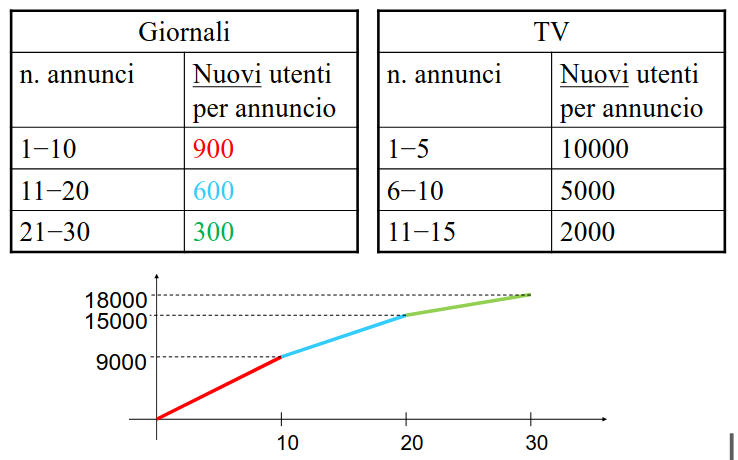
\includegraphics[width=0.5\linewidth]{pubblicita.png}
\end{figure}

\noindent Si definiscono variabili intere per le singole fasce $G_1, G_2, G_3$ (per i giornali) e $T_1, T_2, T_3$ (per la TV).
Il modello lineare intero è:
\[
\begin{aligned}
\max \quad & 900 G_1 + 600 G_2 + 300 G_3 + 10000 T_1 + 5000 T_2 + 2000 T_3 \\
\text{s.t.} \quad & G_1 + G_2 + G_3 + 10 T_1 + 10 T_2 + 10 T_3 \le 150 \quad \text{(Vincolo Budget in K€)} \\
& G_1, G_2, G_3 \le 10 \\
& T_1, T_2, T_3 \le 5 \\
& G_1, G_2, G_3, T_1, T_2, T_3 \ge 0, \text{ INTERE}
\end{aligned}
\]

\subsubsection{Altri Modelli PLI Notevoli}

\paragraph{Variante KP: Bounded Knapsack Problem (KP-bounded)}
A differenza dello Zaino classico (variabili binarie), qui il generico oggetto $i$ è disponibile in $p_i$ esemplari.
Le variabili diventano quantitative intere $x_i$, rappresentanti il numero di copie scelte.
\[
\begin{aligned}
\text{(KP-b)} \quad \max \quad & \sum_{i=1}^n c_i x_i \\
\text{s.t.} \quad & \sum_{i=1}^n a_i x_i \le b \\
& 0 \le x_i \le p_i \quad \text{INTERA} \quad i=1,\dots,n
\end{aligned}
\]

\paragraph{Variante KP: Subset-sum Problem (SSP)}
Dato un insieme di $n$ numeri, se ne vuole selezionare un sottoinsieme la cui somma sia massima ma non ecceda una certa soglia $b$. In questo caso, il profitto dell'oggetto coincide col suo peso ($a_i = c_i$). Questo modello è molto usato nel taglio di barre per minimizzare lo scarto.
\[
\begin{aligned}
\text{(SSP)} \quad \max \quad & \sum_{i=1}^n c_i x_i \\
\text{s.t.} \quad & \sum_{i=1}^n c_i x_i \le b \\
& x_i \in \{0,1\} \quad i=1,\dots,n
\end{aligned}
\]

\paragraph{Problema KP Multiplo (MKP)}
Invece di un solo zaino, abbiamo $m$ contenitori, ciascuno con la propria capacità $b_j$ ($j=1,\dots,m$). Ogni oggetto $i$ può andare al più in un solo contenitore.
Definiamo $x_{ij} = 1$ se l'oggetto $i$ va nel contenitore $j$, $0$ altrimenti.
\[
\begin{aligned}
\text{(MKP)} \quad \max \quad & \sum_{i=1}^n \sum_{j=1}^m c_i x_{ij} \\
\text{s.t.} \quad & \sum_{j=1}^m x_{ij} \le 1 \quad i=1,\dots,n \quad \text{(al più 1 contenitore per oggetto)} \\
& \sum_{i=1}^n a_i x_{ij} \le b_j \quad j=1,\dots,m \quad \text{(rispetto capacità per ogni zaino)} \\
& x_{ij} \in \{0,1\} \quad i=1,\dots,n; \: j=1,\dots,m
\end{aligned}
\]

\paragraph{Bin Packing Problem (BPP)}
Abbiamo $n$ oggetti di peso $a_i$ e un numero virtualmente infinito di contenitori identici (ma all'atto pratico ne serviranno al massimo $n$), tutti di capacità fissata $b$.
L'obiettivo è impaccare \textbf{tutti} gli oggetti utilizzando il \textbf{minor numero possibile} di contenitori.
Usiamo le stesse $x_{ij}$ per indicare se l'oggetto $i$ è nel bin $j$, più una variabile $y_j = 1$ se il contenitore $j$ è utilizzato (aperto), $0$ altrimenti.
\[
\begin{aligned}
\text{(BPP)} \quad \min \quad & \sum_{j=1}^n y_j \\
\text{s.t.} \quad & \sum_{j=1}^n x_{ij} = 1 \quad i=1,\dots,n \quad \text{(tutti gli oggetti devono essere impaccati)} \\
& \sum_{i=1}^n a_i x_{ij} \le b y_j \quad j=1,\dots,n \quad \text{(la capacità si attiva solo se } y_j=1) \\
& x_{ij} \in \{0,1\}, \: y_j \in \{0,1\}
\end{aligned}
\]

\subparagraph{Variante BPP: Vector Packing (VPP)}
Se gli oggetti presentano più di una dimensione (es. oltre al peso $a_i$, occupano un volume $v_i$), si aggiungono semplicemente dei vincoli supplementari di capacità per ogni contenitore. Ad esempio:
\[
\sum_{i=1}^n v_i x_{ij} \le V y_j \quad j=1,\dots,n
\]

\subparagraph{Variante BPP: Bin con capacità variabile}
Se i contenitori non sono identici, ma ciascuno possiede una propria capacità $b_j$ ed un proprio costo fisso di utilizzo $c_j$, la funzione obiettivo diventa $\min \sum c_j y_j$ e la limitazione di capacità dell'imballaggio si adatta in $\sum_{i=1}^n a_i x_{ij} \le b_j y_j$.

\newpage

\subsection{Esercizi Svolti di Modellazione}

Gli esercizi che seguono sono del tipo proposto nelle esercitazioni e nella prova scritta: non si chiede di \textit{risolvere} il problema, ma di \textbf{formularlo} come modello di PL/PLI. Per ognuno seguiremo sempre lo stesso schema di lavoro:
\begin{enumerate}
    \item \textbf{Dati}: insiemi di indici e parametri noti (comprese le matrici di incidenza booleane che il testo descrive a parole);
    \item \textbf{Variabili decisionali}: significato a parole e dominio ($\ge 0$, intera, binaria);
    \item \textbf{Funzione obiettivo};
    \item \textbf{Vincoli}, uno per riga e sempre quantificati;
    \item \textbf{Verifica di linearità}: nessun prodotto tra variabili, nessuna frazione con variabili al denominatore, nessun $\max$/$\min$ o valore assoluto lasciato "grezzo".
\end{enumerate}

\subsubsection{Esercizio 1: Selezione di un team di sviluppo}
\textit{Un'azienda deve formare un team di sviluppo scegliendo tra $m$ candidati. Il progetto richiede $n$ linguaggi di programmazione e per ogni candidato si sa quali linguaggi conosce. Si vuole selezionare il minor numero possibile di candidati in modo che ogni linguaggio richiesto sia conosciuto da almeno un membro del team.}\\

\noindent\textbf{Dati.} Insieme dei linguaggi $i \in \{1,\dots,n\}$, insieme dei candidati $j \in \{1,\dots,m\}$ e la matrice di conoscenza
\[
b_{ij} = \begin{cases} 1 & \text{se il candidato } j \text{ conosce il linguaggio } i\\ 0 & \text{altrimenti}\end{cases}
\]

\noindent\textbf{Variabili.} La decisione è "prendo o non prendo il candidato $j$": una variabile logica per candidato.
\[
y_j = \begin{cases} 1 & \text{se il candidato } j \text{ viene selezionato}\\ 0 & \text{altrimenti}\end{cases} \quad j=1,\dots,m
\]

\noindent\textbf{Funzione obiettivo.} Minimizzare la cardinalità del team: contare i selezionati significa sommare le variabili logiche.
\[
\min \sum_{j=1}^m y_j
\]

\noindent\textbf{Vincoli.} Per ogni linguaggio deve esserci \textit{almeno un} selezionato che lo conosce. La somma $\sum_j b_{ij}y_j$ conta esattamente quanti membri del team conoscono il linguaggio $i$ (i candidati che non lo conoscono danno contributo nullo perché $b_{ij}=0$):
\[
\sum_{j=1}^m b_{ij} y_j \ge 1 \quad i=1,\dots,n \hspace{1cm} y_j \in \{0,1\} \quad j=1,\dots,m
\]

\noindent\textbf{Commento.} È un \textbf{Set Covering} puro con costi tutti unitari ($c_j=1$): l'insieme da coprire $N$ è quello dei linguaggi, e il sottoinsieme $F_j$ associato al candidato $j$ è l'insieme dei linguaggi che egli conosce. Riconoscere il modello noto è ciò che l'esercizio chiede davvero.

\paragraph{Varianti tipiche}
\begin{itemize}
    \item \textit{Ogni linguaggio deve essere coperto da almeno $k_i$ persone} (ridondanza): $\sum_j b_{ij}y_j \ge k_i$.
    \item \textit{Ogni candidato ha un costo $c_j$ e si minimizza la spesa}: la funzione obiettivo diventa $\min \sum_j c_j y_j$ (Set Covering generale).
    \item \textit{Due candidati $h$ e $k$ non possono lavorare insieme}: $y_h + y_k \le 1$.
    \item \textit{Se si prende il candidato $h$ occorre prendere anche il candidato $k$} (implicazione $h \Rightarrow k$): $y_k \ge y_h$.
\end{itemize}

\subsubsection{Esercizio 2: Piano di studi}
\textit{Uno studente deve scegliere i corsi del proprio piano di studi tra $n$ corsi disponibili. Ogni corso $i$ vale $C_i$ crediti e ha un indice di difficoltà $t_i$; l'insieme $I$ contiene i corsi che lo studente ritiene interessanti. Alcuni corsi sono propedeutici: se si sceglie il corso $i$, occorre inserire anche tutti i corsi dell'insieme $G_i$. Il piano deve valere esattamente 120 crediti e la difficoltà media dei corsi scelti non deve superare una soglia $K$. Si vuole massimizzare il numero di corsi interessanti inseriti.}\\

\noindent\textbf{Dati.} $C_i$ crediti, $t_i$ difficoltà, $G_i \subseteq \{1,\dots,n\}$ insieme dei corsi propedeutici ad $i$, $I \subseteq \{1,\dots,n\}$ corsi interessanti, soglia $K$.

\noindent\textbf{Variabili.}
\[
x_i = \begin{cases} 1 & \text{se il corso } i \text{ viene inserito nel piano}\\ 0 & \text{altrimenti}\end{cases} \quad i=1,\dots,n
\]

\noindent\textbf{Funzione obiettivo.} Si contano solo i corsi interessanti, cioè si somma su $I$:
\[
\max \sum_{i \in I} x_i
\]

\noindent\textbf{Vincoli.}
\begin{itemize}
    \item \textbf{Crediti}: $\displaystyle\sum_{i=1}^n C_i x_i = 120$.
    \item \textbf{Propedeuticità}: se scelgo $i$ devo scegliere anche ogni $j \in G_i$. È l'implicazione logica $x_i \implies x_j$, che si scrive
    \[
    x_i \le x_j \quad i=1,\dots,n, \; \forall j \in G_i
    \]
    Si noti il verso: se $x_i=1$ allora $x_j$ è forzata a $1$; se $x_i=0$, $x_j$ resta libera (posso seguire il corso propedeutico anche senza seguire $i$).
    \item \textbf{Difficoltà media}. Il testo dice "media", quindi la scrittura immediata sarebbe
    \[
    \frac{\sum_{i=1}^n t_i x_i}{\sum_{i=1}^n x_i} \le K
    \]
    che \textbf{non è lineare}, avendo variabili al denominatore. Poiché il denominatore è certamente positivo (almeno un corso viene scelto), si può moltiplicare entrambi i membri per esso senza cambiare il verso della disuguaglianza:
    \[
    \sum_{i=1}^n t_i x_i \le K \sum_{i=1}^n x_i \quad\Longleftrightarrow\quad \sum_{i=1}^n (t_i - K)\, x_i \le 0
    \]
    Questa è la forma da consegnare: lineare e con un solo termine per variabile.
    \item $x_i \in \{0,1\}$, $i=1,\dots,n$.
\end{itemize}

\noindent\textbf{Commento.} La struttura di base è quella dello \textbf{zaino} (selezione di elementi con un vincolo di capacità, qui sui crediti), arricchita da vincoli di implicazione e da un vincolo di media. Il passaggio da media a forma lineare è il punto che l'esercizio vuole verificare.

\subsubsection{Esercizio 3: Composizione dei team con vincoli di quota}
\textit{Un'azienda deve assegnare $n$ candidati a $m$ team. Ogni candidato $i$ ha un'età $e_i$ e un costo annuo $c_i$; l'insieme $D$ contiene i candidati di sesso femminile. Ogni candidato va assegnato ad un solo team, ogni team $j$ deve avere almeno $t_j$ persone e almeno metà dei componenti di ciascun team deve appartenere a $D$. Minimizzare il costo totale.}\\

\noindent\textbf{Variabili.} Si tratta di un'assegnazione oggetti$\to$luoghi:
\[
x_{ij} = \begin{cases} 1 & \text{se il candidato } i \text{ è assegnato al team } j\\ 0 & \text{altrimenti}\end{cases} \quad i=1,\dots,n; \; j=1,\dots,m
\]

\noindent\textbf{Modello.}
\[
\begin{aligned}
\min \quad & \sum_{i=1}^n \sum_{j=1}^m c_i x_{ij} \\
\text{s.t.} \quad & \sum_{j=1}^m x_{ij} = 1 & i=1,\dots,n \hspace{0.5cm}\text{(semi-assegnamento)}\\
& \sum_{i=1}^n x_{ij} \ge t_j & j=1,\dots,m \hspace{0.5cm}\text{(dimensione minima)}\\
& \sum_{i \in D} x_{ij} \ge \tfrac{1}{2}\sum_{i=1}^n x_{ij} & j=1,\dots,m \hspace{0.5cm}\text{(quota)}\\
& x_{ij} \in \{0,1\}
\end{aligned}
\]

\noindent\textbf{Spiegazione del vincolo di quota.} "Almeno metà del team appartiene a $D$" è di nuovo un vincolo di proporzione: si confronta il numero di componenti in $D$ del team $j$, cioè $\sum_{i\in D}x_{ij}$, con la metà della numerosità del team, $\frac{1}{2}\sum_{i}x_{ij}$. Entrambi i membri sono lineari, quindi il vincolo è già ammissibile; portandolo a sinistra si ottiene la forma equivalente $\sum_{i\in D} x_{ij} - \sum_{i \notin D} x_{ij} \ge 0$.

\noindent\textbf{Estensione: differenza d'età.} Se si chiede in aggiunta che \textit{in ogni team la differenza d'età tra il più giovane e il più anziano non superi $\Delta$}, si usano i \textbf{vincoli di soglia}: si introducono due variabili quantitative per team, $u_j$ (età massima) e $l_j$ (età minima), e si impone
\[
u_j \ge e_i x_{ij}, \hspace{1cm} l_j \le e_i x_{ij} + M(1-x_{ij}), \hspace{1cm} u_j - l_j \le \Delta
\]
per ogni $i$ e $j$. Il termine $M(1-x_{ij})$ (con $M$ pari all'età massima) serve a \textbf{disattivare} il vincolo su $l_j$ per i candidati non assegnati al team $j$: senza di esso $l_j$ verrebbe schiacciata a zero da tutti i candidati esterni.

\subsubsection{Esercizio 4: Acquisti con sconto a soglia}
\textit{Un'azienda deve acquistare $n$ prodotti, ciascuno con un costo $c_j$, presso $k$ possibili aziende fornitrici. Ogni prodotto va acquistato una sola volta e ogni azienda $o$ vende solo un certo sottoinsieme di prodotti. Se la spesa presso l'azienda $o$ supera la soglia $g_o$, essa applica uno sconto complessivo $s_o$. Minimizzare la spesa.}\\

\noindent\textbf{Dati.} $d_{jo} = 1$ se il prodotto $j$ è venduto dall'azienda $o$; $c_j$ costo del prodotto $j$; $g_o$ soglia; $s_o$ sconto.

\noindent\textbf{Variabili.} Servono due famiglie di variabili: una \textit{decisionale} per gli acquisti e una \textit{ausiliaria} per registrare l'attivazione dello sconto.
\[
x_{jo} = \begin{cases} 1 & \text{se il prodotto } j \text{ è acquistato dall'azienda } o\\ 0 & \text{altrimenti}\end{cases}
\hspace{1cm}
y_o = \begin{cases} 1 & \text{se l'azienda } o \text{ concede lo sconto}\\ 0 & \text{altrimenti}\end{cases}
\]

\noindent\textbf{Modello.}
\[
\begin{aligned}
\min \quad & \sum_{o=1}^k \sum_{j=1}^n c_j x_{jo} - \sum_{o=1}^k s_o y_o \\
\text{s.t.} \quad & \sum_{o=1}^k x_{jo} = 1 & j=1,\dots,n \hspace{0.5cm}\text{(ogni prodotto acquistato una volta)}\\
& x_{jo} \le d_{jo} & j=1,\dots,n; \; o=1,\dots,k \hspace{0.5cm}\text{(disponibilità)}\\
& \sum_{j=1}^n c_j x_{jo} \ge g_o\, y_o & o=1,\dots,k \hspace{0.5cm}\text{(legame sconto--spesa)}\\
& x_{jo}, y_o \in \{0,1\}
\end{aligned}
\]

\noindent\textbf{Spiegazione del legame logico.} Il vincolo $\sum_j c_j x_{jo} \ge g_o y_o$ è la traduzione lineare dell'implicazione "\textit{sconto attivo} $\implies$ \textit{soglia raggiunta}":
\begin{itemize}
    \item se $y_o = 1$ il vincolo diventa $\sum_j c_j x_{jo} \ge g_o$, cioè lo sconto si può prendere solo avendo speso abbastanza;
    \item se $y_o = 0$ il vincolo diventa $\sum_j c_j x_{jo} \ge 0$, cioè è inattivo.
\end{itemize}
Non serve imporre l'altra metà dell'implicazione (soglia raggiunta $\implies$ sconto attivo): trattandosi di una minimizzazione in cui lo sconto compare con segno negativo, l'ottimo porrà sempre $y_o=1$ quando ne ha diritto. È esattamente lo stesso ragionamento del \textbf{costo fisso di produzione}, con i segni invertiti.

\subsubsection{Esercizio 5: Polizze assicurative per una flotta}
\textit{Una ditta ha $n$ camion; il camion $i$ deve percorrere almeno $m_i$ chilometri all'anno e la flotta deve percorrere complessivamente $Q$ chilometri. La polizza del camion $i$ costa $c_i$ se esso percorre al più $k_i$ chilometri, altrimenti costa $d_i$ (con $d_i > c_i$). Minimizzare il costo totale delle polizze.}\\

\noindent\textbf{Variabili.} Una quantitativa per i chilometri e una logica per la fascia tariffaria:
\[
w_i \ge 0 = \text{chilometri percorsi dal camion } i
\hspace{1cm}
z_i = \begin{cases} 1 & \text{se il camion } i \text{ resta entro } k_i \text{ km}\\ 0 & \text{altrimenti}\end{cases}
\]

\noindent\textbf{Modello.}
\[
\begin{aligned}
\min \quad & \sum_{i=1}^n \Big( c_i z_i + d_i (1-z_i) \Big) \\
\text{s.t.} \quad & w_i \ge m_i & i=1,\dots,n \\
& w_i \le k_i z_i + M_i (1-z_i) & i=1,\dots,n \\
& \sum_{i=1}^n w_i = Q \\
& w_i \ge 0, \; z_i \in \{0,1\}
\end{aligned}
\]

\noindent\textbf{Spiegazione.} La funzione di costo è \textbf{a gradini}, dunque discontinua: si tratta della stessa situazione del carico fisso, gestita con una variabile logica che seleziona il tratto. Il vincolo di legame va letto per casi:
\begin{itemize}
    \item se $z_i = 1$ diventa $w_i \le k_i$: si paga $c_i$ e si è obbligati a restare sotto soglia;
    \item se $z_i = 0$ diventa $w_i \le M_i$: si paga $d_i$ e il chilometraggio è libero (con $M_i$ pari a un upper bound sui chilometri percorribili, ad esempio $Q$).
\end{itemize}
Anche qui non occorre forzare $z_i=1$ quando $w_i \le k_i$: essendo $c_i < d_i$ e il problema di minimo, l'ottimo sceglierà da solo la tariffa più conveniente compatibile con i chilometri.

\subsubsection{Esercizio 6: Fornitura di energia con quantità minima}
\textit{Un'azienda ha un fabbisogno mensile di $Q$ kWh e può rifornirsi da $n$ fornitori. Il fornitore $i$ applica un prezzo $p_i$ per kWh, richiede un ordine minimo di $m_i$ kWh e chiede un canone fisso $F_i$ se viene utilizzato. Minimizzare la spesa.}\\

\noindent\textbf{Variabili.}
\[
x_i \ge 0 = \text{kWh acquistati dal fornitore } i
\hspace{1cm}
y_i = \begin{cases} 1 & \text{se si usa il fornitore } i\\ 0 & \text{altrimenti}\end{cases}
\]

\noindent\textbf{Modello.}
\[
\begin{aligned}
\min \quad & \sum_{i=1}^n \big( p_i x_i + F_i y_i \big) \\
\text{s.t.} \quad & \sum_{i=1}^n x_i = Q \\
& m_i y_i \le x_i \le M y_i & i=1,\dots,n \\
& x_i \ge 0, \; y_i \in \{0,1\}
\end{aligned}
\]

\noindent\textbf{Spiegazione.} Il doppio vincolo $m_i y_i \le x_i \le M y_i$ è la \textbf{minima quantità positiva}: costringe $x_i$ ad appartenere all'insieme non convesso $\{0\} \cup [m_i, M]$.
\begin{itemize}
    \item Se $y_i = 0$: $0 \le x_i \le 0$, quindi $x_i = 0$ e non si paga il canone.
    \item Se $y_i = 1$: $m_i \le x_i \le M$, quindi si rispetta l'ordine minimo e si paga il canone $F_i$.
\end{itemize}
Come upper bound $M$ conviene usare $Q$, che è il massimo acquistabile da un singolo fornitore: è il valore più stretto disponibile ed evita rilassamenti inutilmente deboli.

\subsubsection{Esercizio 7: Dislocazione del personale su più sedi}
\textit{Un'azienda deve distribuire $n$ dipendenti su $S$ sedi, con al più $p$ dipendenti per sede. Per ogni coppia di dipendenti $(i,j)$ è noto il tempo $t_{ij}$ di interazione a distanza che si genera se i due lavorano in sedi diverse. Minimizzare il tempo totale di interazione a distanza.}\\

\noindent\textbf{Variabili.}
\[
x_{is} = \begin{cases} 1 & \text{se il dipendente } i \text{ è assegnato alla sede } s\\ 0 & \text{altrimenti}\end{cases}
\hspace{1cm}
y_{ij} = \begin{cases} 1 & \text{se } i \text{ e } j \text{ sono in sedi diverse}\\ 0 & \text{altrimenti}\end{cases}
\]

\noindent\textbf{Modello.}
\[
\begin{aligned}
\min \quad & \sum_{i=1}^{n-1}\sum_{j=i+1}^{n} t_{ij}\, y_{ij} \\
\text{s.t.} \quad & \sum_{s=1}^{S} x_{is} = 1 & i=1,\dots,n \\
& \sum_{i=1}^n x_{is} \le p & s=1,\dots,S \\
& y_{ij} \ge x_{is} - x_{js} & \forall i<j, \; s=1,\dots,S \\
& y_{ij} \ge x_{js} - x_{is} & \forall i<j, \; s=1,\dots,S \\
& x_{is}, y_{ij} \in \{0,1\}
\end{aligned}
\]

\noindent\textbf{Spiegazione del legame.} La condizione da esprimere è "$y_{ij}=1$ se esiste una sede occupata da uno solo dei due dipendenti". Se $i$ è nella sede $s$ e $j$ non lo è, la prima disuguaglianza dà $y_{ij}\ge 1-0=1$; simmetricamente per il caso opposto. Se invece i due stanno nella stessa sede, tutte le differenze sono nulle o negative e la minimizzazione (con $t_{ij}\ge0$) pone $y_{ij}=0$. Non serve quindi imporre l'altra metà della relazione logica.

\noindent\textbf{Perché servono le variabili di coppia.} Se si provasse a scrivere direttamente il costo si otterrebbe un termine del tipo $t_{ij}\,(1 - \sum_s x_{is}x_{js})$: c'è un \textbf{prodotto tra variabili}, quindi il modello non sarebbe lineare. Le $y_{ij}$ sono variabili \textbf{ausiliarie} che linearizzano quel prodotto, esattamente come le $y_j$ del costo fisso linearizzano una funzione discontinua. Se invece servisse la condizione "\textit{stessa} sede" (ad esempio per premiare le coppie affiatate), la linearizzazione dell'AND darebbe
\[
w_{ij} \ge x_{is} + x_{js} - 1 \quad \forall s
\]

\subsubsection{Esercizio 8: Asta di automobili}
\textit{Un concessionario deve vendere $n$ automobili e riceve $m$ offerte. L'offerta $j$ propone di acquistare in blocco l'insieme di automobili $S_j$ al prezzo $p_j$ e non è frazionabile. Ogni automobile può essere venduta al più una volta. Massimizzare il ricavo.}\\

\noindent\textbf{Variabili.}
\[
x_j = \begin{cases} 1 & \text{se l'offerta } j \text{ viene accettata}\\ 0 & \text{altrimenti}\end{cases} \quad j=1,\dots,m
\]

\noindent\textbf{Modello.}
\[
\begin{aligned}
\max \quad & \sum_{j=1}^m p_j x_j \\
\text{s.t.} \quad & \sum_{j : i \in S_j} x_j \le 1 & i=1,\dots,n \\
& x_j \in \{0,1\}
\end{aligned}
\]

\noindent\textbf{Commento.} È un \textbf{Set Packing}: ogni automobile (elemento di $N$) può comparire in \textit{al più un} sottoinsieme selezionato. Coerentemente con quanto visto nella teoria, il problema è di massimo: formulato come minimo con prezzi positivi, la soluzione banale sarebbe non accettare nessuna offerta. Se il concessionario fosse obbligato a vendere tutte le automobili, il vincolo diventerebbe $\sum_{j: i \in S_j} x_j = 1$ e il problema sarebbe un \textbf{Set Partitioning}.

\subsubsection{Esercizio 9: Assegnazione di fotocopiatrici ai reparti}
\textit{Un'azienda ha $n$ reparti e $m$ modelli di fotocopiatrice. La fotocopiatrice $i$ costa $c_i$ al mese e produce al massimo $f_i$ stampe al mese; il reparto $j$ necessita di $v_j$ fotocopie al mese e non può ospitare più di 3 fotocopiatrici. Minimizzare il costo mensile.}\\

\noindent\textbf{Variabili.} Qui la decisione è \textit{quante} macchine di ciascun modello mettere in ciascun reparto: variabili quantitative \textbf{intere}, non binarie.
\[
x_{ij} \ge 0 \text{ intera} = \text{numero di fotocopiatrici del modello } i \text{ assegnate al reparto } j
\]

\noindent\textbf{Modello.}
\[
\begin{aligned}
\min \quad & \sum_{i=1}^m \sum_{j=1}^n c_i x_{ij} \\
\text{s.t.} \quad & \sum_{i=1}^m f_i x_{ij} \ge v_j & j=1,\dots,n \hspace{0.5cm}\text{(fabbisogno del reparto)}\\
& \sum_{i=1}^m x_{ij} \le 3 & j=1,\dots,n \hspace{0.5cm}\text{(spazio disponibile)}\\
& x_{ij} \ge 0 \text{ INTERE}
\end{aligned}
\]

\noindent\textbf{Commento.} L'errore più frequente è dichiarare $x_{ij} \in \{0,1\}$ per abitudine: il testo consente più macchine dello stesso modello nello stesso reparto, quindi il dominio corretto è quello intero. La struttura è quella di un \textbf{KP-bounded} replicato per reparto, con vincolo di copertura del fabbisogno al posto della capacità.

\subsubsection{Esercizio 10: Commesse e macchine saldatrici}
\textit{Un'officina dispone di $m$ saldatrici e ha ricevuto $n$ commesse. La commessa $i$ frutta un guadagno $g_i$ se evasa e comporta una penale $p_i$ se rifiutata; per essere evasa richiede $t_{ij}$ giorni di lavoro sulla macchina $j$. Ogni macchina è disponibile per $T$ giorni. Massimizzare il profitto.}\\

\noindent\textbf{Variabili.}
\[
y_i = \begin{cases} 1 & \text{se la commessa } i \text{ viene evasa}\\ 0 & \text{altrimenti}\end{cases}
\hspace{1cm}
x_{ij} = \begin{cases} 1 & \text{se la commessa } i \text{ è lavorata sulla macchina } j\\ 0 & \text{altrimenti}\end{cases}
\]

\noindent\textbf{Modello.}
\[
\begin{aligned}
\max \quad & \sum_{i=1}^n \Big( g_i y_i - p_i (1-y_i) \Big) \\
\text{s.t.} \quad & \sum_{j=1}^m x_{ij} = y_i & i=1,\dots,n \\
& \sum_{i=1}^n t_{ij}\, x_{ij} \le T & j=1,\dots,m \\
& x_{ij}, y_i \in \{0,1\}
\end{aligned}
\]

\noindent\textbf{Spiegazione.}
\begin{itemize}
    \item Il vincolo $\sum_j x_{ij} = y_i$ è un semi-assegnamento "condizionato": se la commessa è evasa ($y_i=1$) va assegnata ad esattamente una macchina, se è rifiutata ($y_i=0$) non occupa nessuna macchina. Scrivere $\sum_j x_{ij}=1$ renderebbe impossibile rifiutare le commesse.
    \item La funzione obiettivo mescola guadagni e penali. Sviluppandola si ottiene
    \[
    \sum_{i=1}^n (g_i + p_i)\, y_i - \underbrace{\sum_{i=1}^n p_i}_{\text{costante}}
    \]
    e poiché una costante additiva non cambia l'insieme delle soluzioni ottime (cambia solo il valore ottimo), si può equivalentemente massimizzare $\sum_i (g_i+p_i)y_i$. Questa semplificazione è spesso apprezzata in sede d'esame.
\end{itemize}

\subsubsection{Archetipi ricorrenti nei temi d'esame}
L'esercizio 1 dello scritto vale 8 punti ed è sempre una formulazione PLI da costruire a partire da un testo discorsivo. I testi cambiano, la struttura no: quasi tutti gli esercizi sono una combinazione di tre archetipi.

\paragraph{Archetipo A --- Caricamento/impaccamento con contenitori eterogenei}
Si devono assegnare oggetti (pallet, fusti, lavori) a contenitori (camion, macchine, bin) di capacità $b_i$ e costo di utilizzo $c_i$, massimizzando il profitto netto. Con $x_{ij}=1$ se l'oggetto $j$ va nel contenitore $i$ e $y_i=1$ se il contenitore $i$ è utilizzato:
\[
\max \sum_i \sum_j p_j x_{ij} - \sum_i c_i y_i
\hspace{0.8cm}
\sum_i x_{ij} \le 1 \;\; \forall j
\hspace{0.8cm}
\sum_j w_j x_{ij} \le b_i y_i \;\; \forall i
\]
Due punti che valgono da soli metà esercizio:
\begin{itemize}
    \item il semi-assegnamento è $\le 1$ e non $=1$ ogni volta che il testo dice "\textit{un sottoinsieme} di oggetti", "non tutti devono essere caricati";
    \item il vincolo $\sum_j w_j x_{ij} \le b_i y_i$ \textbf{ingloba} sia la capacità sia il legame logico "se carico qualcosa allora il contenitore è usato". In alternativa si scrivono separatamente $\sum_j w_j x_{ij} \le b_i$ e $x_{ij}\le y_i$; entrambe le versioni sono corrette, la prima usa molti meno vincoli.
\end{itemize}

\paragraph{Archetipo B --- Selezione di risorse con costo fisso + costo variabile}
Si sceglie chi assumere/attivare (camerieri, fornitori, impianti) pagando un costo fisso $l_i$ per la risorsa attivata e un costo variabile $v_i$ per ogni unità servita, con un limite di capacità $c_i$ espresso in tempo, peso o quantità:
\[
\min \sum_i \left( l_i y_i + v_i \sum_j x_{ij}\right)
\hspace{0.8cm}
\sum_i x_{ij} = 1 \;\; \forall j
\hspace{0.8cm}
\sum_j p_j x_{ij} \le c_i y_i \;\; \forall i
\]
È il carico fisso applicato a un problema di assegnamento: la parte fissa moltiplica la variabile logica, quella variabile moltiplica le variabili di assegnamento.

\paragraph{Archetipo C --- Assegnamento con molteplicità e incompatibilità}
Ogni lavoro $j$ deve essere svolto da \textbf{esattamente $p_j$} macchine, ogni macchina $i$ ne esegue \textbf{al più $q_i$}, ed è data una lista $L$ di coppie di lavori che non possono stare sulla stessa macchina:
\[
\min \sum_i \sum_j c_{ij}x_{ij}
\hspace{0.6cm}
\sum_i x_{ij} = p_j \;\; \forall j
\hspace{0.6cm}
\sum_j x_{ij} \le q_i \;\; \forall i
\hspace{0.6cm}
x_{ih} + x_{ik} \le 1 \;\; \forall (h,k)\in L, \forall i
\]
Il vincolo di incompatibilità $x_{ih}+x_{ik}\le 1$ è lo stesso già visto in MCMS per i lavori con intervalli sovrapposti: cambia il modo in cui il testo descrive l'incompatibilità, non il vincolo.

\paragraph{Dizionario testo $\to$ vincolo}
\begin{center}
\begin{tabular}{ll}
\hline
\textbf{Frase nel testo} & \textbf{Vincolo} \\
\hline
"ogni $j$ va assegnato a uno e un solo $i$" & $\sum_i x_{ij} = 1$ \\
"un sottoinsieme di $j$", "se non conveniente si lascia fuori" & $\sum_i x_{ij} \le 1$ \\
"ogni $j$ richiede $p_j$ risorse" & $\sum_i x_{ij} = p_j$ \\
"ogni $i$ può servirne al massimo $q_i$" & $\sum_j x_{ij} \le q_i$ \\
"$h$ e $k$ non possono stare insieme" & $x_{ih} + x_{ik} \le 1$ \\
"se si usa $i$ si paga un costo fisso" & $\sum_j w_j x_{ij} \le b_i y_i$, costo $c_iy_i$ \\
"almeno una quantità minima, oppure niente" & $m_i y_i \le x_i \le M y_i$ \\
"se si sceglie $i$ occorre anche $j$" & $x_i \le x_j$ \\
"al massimo $k$ tra le alternative" & $\sum_{i \in S} x_i \le k$ \\
"il valore medio non superi $K$" & $\sum_i (t_i - K)x_i \le 0$ \\
"minimizzare il massimo (tempo, carico, ritardo)" & $t \ge \sum_j d_j x_{ij}\;\forall i$, $\min t$ \\
\hline
\end{tabular}
\end{center}

\subsubsection{Errori tipici da evitare}
\begin{itemize}
    \item Scrivere prodotti tra variabili decisionali (es. $x_i x_j$, oppure $y\cdot x$ con $y$ binaria e $x$ continua) senza linearizzarli con variabili ausiliarie.
    \item Lasciare variabili al denominatore: ogni vincolo di media, percentuale o quota va moltiplicato per il denominatore.
    \item Usare disuguaglianze \textbf{strette} ($>$, $<$), non ammesse in PL/PLI: per "$x>0$" con $x$ intera si scrive $x \ge 1$, con $x$ continua si usa la minima quantità positiva.
    \item Dimenticare di dichiarare il dominio delle variabili, in particolare l'interezza e la non negatività.
    \item Usare un $M$ enorme quando il problema offre un upper bound naturale e stretto (il rilassamento continuo peggiora e con esso i tempi di calcolo).
    \item Confondere "al più uno" ($\le 1$), "esattamente uno" ($=1$) e "almeno uno" ($\ge 1$): è la differenza tra Set Packing, Set Partitioning e Set Covering.
    \item Modellare un $\max$ (o un $\min$) direttamente in funzione obiettivo invece di introdurre la variabile di soglia con i relativi vincoli, come nel Min Makespan.
\end{itemize}

\newpage

\section{Algoritmi per PL e PLI}

\subsection{Geometria Della Programmazione Lineare}

\paragraph{Qual è la domanda a cui questa sezione risponde?}
Un problema di PL ha \emph{infinite} soluzioni ammissibili (tutti i punti di una regione continua): non possiamo enumerarle. Eppure il simplesso, che vedremo fra poco, risolve la PL \textbf{saltando da un vertice all'altro}, cioè esaminando un numero \emph{finito} di punti. Tutta questa sezione serve a giustificare quel salto, rispondendo a tre domande:
\begin{enumerate}
    \item Che forma ha la regione ammissibile di un problema di PL? (Risposta: è un \textbf{poliedro}.)
    \item Cos'è un "vertice" quando le variabili sono $n>2$ e non possiamo disegnare? (Risposta: è una \textbf{soluzione di base ammissibile}, un oggetto puramente algebrico che sappiamo calcolare risolvendo un sistema lineare.)
    \item Perché è lecito cercare l'ottimo solo fra i vertici? (Risposta: il \textbf{Teorema di Motzkin} + la \textbf{proprietà fondamentale della PL}.)
\end{enumerate}
Se si tiene a mente questo filo conduttore, le definizioni che seguono smettono di sembrare arbitrarie: ognuna è un pezzo di quella dimostrazione.

\medskip
\noindent La Programmazione Lineare (PL) e la Programmazione Lineare Intera (PLI) sono casi particolari della più generale Programmazione Lineare Mista (PLM).

\subsubsection{Un Esempio e la Restrizione dello Spazio di Ricerca}
Consideriamo il seguente problema di massimizzazione a due variabili, che useremo come \textbf{esempio guida} per tutta la sezione:
\[
\begin{aligned}
\max \quad & z = x + y \\
\text{s.t.} \quad & x + 2y \ge 2 \\
& x \le 3 \\
& y \le 2 \\
& x, y \ge 0
\end{aligned}
\]
\noindent Rappresentando graficamente i vincoli nel piano cartesiano $\mathbb{R}^2$, si ottiene una regione ammissibile a forma di poligono.

\begin{figure}[h!]
    \centering
    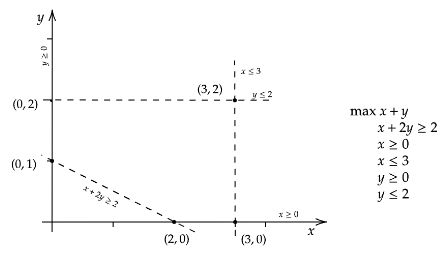
\includegraphics[width=0.5\linewidth]{esempioPL.png}
\end{figure}

\noindent Ogni vincolo taglia il piano in due e ne tiene metà; l'intersezione delle cinque metà (i cinque vincoli, contando anche $x\ge0$ e $y\ge0$) è il poligono ammissibile. I suoi angoli sono:
\[ (2,0),\quad (3,0),\quad (3,2),\quad (0,2),\quad (0,1). \]
Valutando $z=x+y$ solo su questi cinque punti si ottiene $2,\;3,\;\mathbf{5},\;2,\;1$: l'ottimo è $z^*=5$ in $(3,2)$. Non abbiamo controllato gli infiniti punti interni, eppure la risposta è corretta.

\paragraph{Perché funziona (intuizione geometrica).}
La funzione obiettivo $z=x+y$ ha \textbf{curve di livello} che sono rette parallele ($x+y=k$). Massimizzare significa traslare questa retta nella direzione del vettore dei costi $c=(1,1)$ finché si può. L'ultimo contatto con il poligono, prima di uscirne, avviene \emph{sempre} in un angolo (o, nel caso degenere in cui la retta di livello è parallela a un lato, lungo un intero lato --- e allora anche i due angoli di quel lato sono ottimi). Quindi: \textbf{se un ottimo esiste, esiste anche in un vertice}.

\medskip
\noindent Morale: lo spazio di ricerca della PL è in linea di principio \textbf{infinito} (ha la cardinalità del continuo), ma può essere ristretto all'insieme \textbf{finito} dei vertici del poliedro. Il resto della sezione serve a \textbf{generalizzare} questo argomento, che in $\mathbb{R}^2$ si "vede", al caso $n>2$ dove disegnare non è possibile e serve l'algebra lineare.

\subsubsection{Nozioni Preliminari}

\paragraph{Iperpiano e Semispazio}
\begin{itemize}
    \item \textbf{Iperpiano}: è l'insieme $\{x \in \mathbb{R}^n \mid ax = b\}$ delle soluzioni dell'equazione lineare $ax = b$, dove $a \in \mathbb{R}^n$ e $b \in \mathbb{R}$. In $\mathbb{R}^2$ rappresenta una retta, in $\mathbb{R}^3$ un piano; in generale è un oggetto di dimensione $n-1$, cioè "una dimensione in meno" dello spazio in cui vive.
    \item \textbf{Semispazio}: è l'insieme $\{x \in \mathbb{R}^n \mid ax \le b\}$ delle soluzioni della disequazione lineare $ax \le b$, cioè una delle due metà in cui l'iperpiano taglia lo spazio. L'iperpiano costituisce il "confine" (iperpiano di supporto) del corrispondente semispazio.
\end{itemize}
\noindent\textit{Esempio.} Nel problema guida, $x \le 3$ è un semispazio di $\mathbb{R}^2$: la metà di piano a sinistra della retta verticale $x=3$, che ne è l'iperpiano di supporto.

\paragraph{Poliedro}
Un \textbf{poliedro} $P$ è definito come l'intersezione di un numero finito $m$ di semispazi. Devono quindi esistere una matrice $A \in \mathbb{R}^{m \times n}$ e un vettore $b \in \mathbb{R}^m$ tali che:
\[ P = \{x \mid Ax \le b\} \]
Ogni riga $A_i x \le b_i$ della matrice è un vincolo, cioè un semispazio: \textbf{la regione ammissibile di un qualsiasi problema di PL è un poliedro}, ed è per questo che studiamo i poliedri.

\noindent\textit{Esempio (forma matriciale del problema guida).} Portiamo tutti i vincoli nel verso $\le$: la disuguaglianza $x+2y\ge2$ diventa $-x-2y\le-2$, e $x\ge0,\;y\ge0$ diventano $-x\le0,\;-y\le0$. Con $m=5$ vincoli e $n=2$ variabili:
\[
A=\begin{pmatrix} -1 & -2 \\ 1 & 0 \\ 0 & 1 \\ -1 & 0 \\ 0 & -1 \end{pmatrix},
\qquad
b=\begin{pmatrix} -2 \\ 3 \\ 2 \\ 0 \\ 0 \end{pmatrix}.
\]
D'ora in poi numeriamo i vincoli $1,\dots,5$ in quest'ordine: 1 è $x+2y\ge2$, 2 è $x\le3$, 3 è $y\le2$, 4 è $x\ge0$, 5 è $y\ge0$.

\paragraph{Insieme Convesso}
Un insieme $C \subseteq \mathbb{R}^n$ è detto \textbf{convesso} se, presi due punti qualsiasi $x, y \in C$, tutto il segmento che li unisce è contenuto in $C$. Formalmente:
\[ \forall x,y \in C, \; \forall \alpha \in [0,1] \implies \alpha x + (1-\alpha)y \in C \]
(al variare di $\alpha$ da $0$ a $1$, il punto $\alpha x + (1-\alpha)y$ percorre esattamente il segmento da $y$ a $x$).
Semispazi e poliedri sono, per definizione, insiemi convessi: intersecare insiemi convessi dà un insieme convesso. Intuitivamente un poliedro non ha "rientranze": è un poligono/solido senza ammaccature.

\subsubsection{Poliedri, Facce e Vertici}

\paragraph{L'idea.} Un poliedro ha parti di dimensione diversa: il corpo pieno, le sue facce piane, i suoi spigoli, i suoi angoli. Vogliamo un modo \textbf{algebrico} (che funzioni anche in $\mathbb{R}^{50}$) per parlarne. Il trucco è: \emph{scegliere un sottoinsieme di vincoli e imporli come uguaglianze}. Più vincoli "blocco" con l'uguale, più mi restringo a una parte piccola del bordo.

\medskip
\noindent Se consideriamo il poliedro $P = \{x \mid Ax \le b\}$ e fissiamo un qualunque sottoinsieme $I \subseteq \{1, \dots, m\}$ (dove $m$ è il numero di vincoli, cioè di righe della matrice), indichiamo:
\begin{itemize}
    \item con $\overline{I}$ il complementare di $I$, ovvero $\{1, \dots, m\} \setminus I$;
    \item con $A_I$ la sottomatrice di $A$ ottenuta considerando solo le righe con indice in $I$;
    \item con $P_I$ il poliedro definito come: $P_I = \{x \mid A_I x = b_I \wedge A_{\overline{I}} x \le b_{\overline{I}}\}$,
\end{itemize}
cioè: i vincoli in $I$ li impongo \textbf{come uguaglianze} (sono "sul bordo"), tutti gli altri restano disuguaglianze.

Se l'insieme $I$ è tale che $P_I$ non è vuoto, allora $P_I$ è detto \textbf{faccia} di $P$.
Il numero di facce distinte di un poliedro è al più $2^m$ (tanti quanti i sottoinsiemi di vincoli). Il poliedro $P$ stesso è considerato una faccia (ovvero $P_\emptyset$: nessun vincolo bloccato). La dimensione di una faccia corrisponde alla dimensione del più piccolo sottospazio in grado di contenerla.

\paragraph{Ma chi sceglie $I$? Nessuno: si scelgono \emph{tutti}.}
Questo è il punto che genera più confusione. $I$ \textbf{non} è un insieme "giusto" da indovinare: la definizione dice che \emph{per ogni} sottoinsieme $I$ dei vincoli, se $P_I \ne \emptyset$ allora $P_I$ è una faccia. Con $m=5$ vincoli ci sono $2^5=32$ scelte possibili di $I$, e ognuna produce una faccia diversa (o l'insieme vuoto, e allora quella scelta si scarta). Negli esempi qui sotto scegliamo $I=\{2\}$, $I=\{2,3\}$, ecc. solo perché sono \emph{campioni} comodi da disegnare: qualunque altro sottoinsieme sarebbe stato altrettanto legittimo, e infatti in fondo li elenchiamo tutti.

\medskip
\noindent Il significato di "mettere $i$ dentro $I$" è: \textbf{obbligo il punto a stare esattamente sul bordo del vincolo $i$}, invece di lasciarlo libero di stare ovunque nella metà di piano ammessa. Quindi:
\begin{center}
\fbox{\parbox{0.92\linewidth}{\centering $I$ = "quali vincoli obbligo a essere stretti (con l'uguale)"\\[2pt] $\overline{I}$ = "quali vincoli lascio come disuguaglianze, cioè liberi di avere margine"}}
\end{center}
Più vincoli metto in $I$, più restringo: da tutto il poligono, a un suo lato, a un suo angolo, fino al vuoto (se chiedo cose incompatibili).

\paragraph{Ricetta: dato $I$, come si calcola $P_I$.}
Non c'è niente da ``capire'' o da indovinare: $I$ è un insieme di \emph{indici di riga}, e l'indice $i$ identifica il vincolo $i$-esimo. Il procedimento è meccanico, in tre passi:

\begin{enumerate}
    \item \textbf{Riscrivi i vincoli con indice in $I$ mettendo l'uguale} al posto di $\le$ (o $\ge$). Ottieni un sistema di $|I|$ equazioni.
    \item \textbf{Risolvi quel sistema}. Tre esiti possibili:
    \begin{itemize}
        \item \emph{incompatibile} $\Rightarrow$ $P_I = \emptyset$, si scarta subito (non è una faccia);
        \item \emph{soluzione unica} (accade quando le equazioni sono $n$ e indipendenti, cioè $\text{rango}(A_I)=n$) $\Rightarrow$ un solo punto candidato;
        \item \emph{infinite soluzioni} (rango $k<n$) $\Rightarrow$ un sottospazio affine di dimensione $n-k$: una retta se $k=n-1$, un piano se $k=n-2$, ecc.
    \end{itemize}
    \item \textbf{Imponi i vincoli rimasti} (quelli in $\overline{I}$, ancora come disuguaglianze) sulle soluzioni trovate al passo 2: ritagliano il pezzo che effettivamente sta dentro il poliedro. Se non ne resta nulla, $P_I=\emptyset$.
\end{enumerate}
Il passo 2 dice \emph{che forma} ha la faccia (punto, segmento/retta, piano\dots), il passo 3 dice \emph{dove comincia e dove finisce}.

\medskip
\noindent\textit{Svolgimento completo con $I=\{1\}$.}
\begin{itemize}
    \item[\textbf{1.}] L'unico vincolo in $I$ è il numero 1, cioè $x+2y\ge2$: lo trasformo in $x+2y=2$.
    \item[\textbf{2.}] Una sola equazione in $n=2$ incognite: rango 1, quindi infinite soluzioni che formano una \textbf{retta} (dimensione $n-k = 2-1 = 1$). Parametrizzo: $x = 2-2y$.
    \item[\textbf{3.}] Impongo i vincoli restanti $\overline{I}=\{2,3,4,5\}$ su quella retta, sostituendo $x=2-2y$:
    \[
    \begin{array}{lll}
    \text{(2) } x\le3: & 2-2y\le3 & \Rightarrow\; y \ge -0{,}5\\
    \text{(3) } y\le2: & & \Rightarrow\; y \le 2\\
    \text{(4) } x\ge0: & 2-2y\ge0 & \Rightarrow\; y \le 1\\
    \text{(5) } y\ge0: & & \Rightarrow\; y \ge 0
    \end{array}
    \]
    Intersecando: $0 \le y \le 1$. La faccia è il segmento $\{(2-2y,\;y) \mid 0\le y\le1\}$, cioè il segmento da $(2,0)$ a $(0,1)$: il \textbf{lato obliquo} del poligono, di dimensione 1.
\end{itemize}

\medskip
\noindent\textit{Svolgimento completo con $I=\{3,4\}$.}
\begin{itemize}
    \item[\textbf{1.}] Vincolo 3 ($y\le2$) $\to$ $y=2$; vincolo 4 ($x\ge0$) $\to$ $x=0$.
    \item[\textbf{2.}] Sistema $\{y=2,\;x=0\}$: due equazioni indipendenti in due incognite (rango $2=n$), soluzione unica $(0,2)$. Dimensione $n-k=0$: è un \textbf{punto}, quindi il candidato vertice.
    \item[\textbf{3.}] Verifico i vincoli rimasti $\overline{I}=\{1,2,5\}$ nel punto $(0,2)$: \;(1) $0+4=4\ge2$ \checkmark; \;(2) $0\le3$ \checkmark; \;(5) $2\ge0$ \checkmark. Tutti soddisfatti $\Rightarrow$ $P_{\{3,4\}}=\{(0,2)\}$ è davvero una faccia, ed è un vertice.
\end{itemize}
Se anche uno solo dei vincoli di $\overline{I}$ fosse stato violato, il punto sarebbe caduto fuori dal poliedro e avremmo concluso $P_I=\emptyset$: è esattamente ciò che accade con $I=\{4,5\}$, che dà $(0,0)$ e viola il vincolo 1.

\medskip
\noindent\textbf{Regola rapida per la dimensione.} Prima ancora di fare i conti del passo 3, il rango $k$ di $A_I$ ti dice cosa aspettarti:
\begin{center}
\begin{tabular}{ccl}
\hline
rango di $A_I$ & dimensione di $P_I$ & che oggetto è (in $\mathbb{R}^2$) \\
\hline
$0$ ($I=\emptyset$) & $2$ & tutto il poliedro \\
$1$ & $1$ & un lato \\
$2 = n$ & $0$ & un vertice \\
\hline
\end{tabular}
\end{center}
Attenzione: $|I|$ e il rango di $A_I$ non coincidono se i vincoli scelti sono ridondanti. Con $I=\{2,4\}$ si ha $|I|=2$ ma le due righe $(1,0)$ e $(-1,0)$ sono proporzionali: rango 1, non 2. Infatti quel sistema non individua un punto --- individua due rette parallele, cioè niente.

\paragraph{E nel verso opposto?} Se invece parti da un punto $x$ del poliedro e ti chiedi \emph{quale} $I$ lo genera, la risposta è l'insieme dei suoi \textbf{vincoli attivi} $I(x)$ (definito poco più avanti): basta sostituire $x$ in tutti i vincoli e segnare quelli soddisfatti con l'uguale. Per $(3,2)$ si trova $I(x)=\{2,3\}$; per un punto interno come $(1{,}5;\,1)$ si trova $I(x)=\emptyset$.

\medskip
\noindent\textit{Esempio (facce del problema guida).} Ricordiamo la numerazione: 1 è $x+2y\ge2$, 2 è $x\le3$, 3 è $y\le2$, 4 è $x\ge0$, 5 è $y\ge0$. In blu la faccia $P_I$ ottenuta, in grigio tratteggiato le rette dei vincoli.

\begin{center}
\begin{minipage}{0.48\linewidth}\centering
\poliguida{
  \fill[blue!35] (2,0)--(3,0)--(3,2)--(0,2)--(0,1)--cycle;
}
\\[2pt] \small $I=\emptyset$ --- nessun vincolo bloccato.\\ $P_\emptyset=P$: tutto il poligono, \textbf{dim.\ 2}.
\end{minipage}\hfill
\begin{minipage}{0.48\linewidth}\centering
\poliguida{
  \draw[blue,line width=2pt] (3,0)--(3,2);
}
\\[2pt] \small $I=\{2\}$ --- blocco solo $x\le3$ in $x=3$.\\ Resta il \textbf{lato} destro, \textbf{dim.\ 1}.
\end{minipage}
\end{center}

\begin{center}
\begin{minipage}{0.48\linewidth}\centering
\poliguida{
  \fill[blue] (3,2) circle (2.6pt);
}
\\[2pt] \small $I=\{2,3\}$ --- blocco $x=3$ \emph{e} $y=2$.\\ Resta il \textbf{vertice} $(3,2)$, \textbf{dim.\ 0}.
\end{minipage}\hfill
\begin{minipage}{0.48\linewidth}\centering
\poliguida{
  \draw[red,line width=1.6pt] (3,-0.5)--(3,2.6);
  \draw[red,line width=1.6pt] (0,-0.5)--(0,2.6);
  \node[red] at (1.5,1.2) {\footnotesize$\emptyset$};
}
\\[2pt] \small $I=\{2,4\}$ --- blocco $x=3$ \emph{e} $x=0$.\\ Rette parallele: $P_I=\emptyset$, \textbf{non è una faccia}.
\end{minipage}
\end{center}

\noindent Si legge così, riga per riga:
\begin{itemize}
    \item $I=\emptyset$: non obbligo nessun vincolo a essere stretto, quindi $P_\emptyset = P$: il poliedro stesso è una faccia (la più grande), di dimensione 2.
    \item $I=\{2\}$: obbligo $x=3$; gli altri quattro vincoli restano $\le$ e ritagliano su quella retta il segmento $0\le y\le 2$. Ottengo il lato verticale $\{(3,y) \mid 0\le y\le 2\}$, di dimensione 1. \emph{Perché proprio il vincolo 2? Per nessun motivo particolare}: scegliendo $I=\{3\}$ avrei ottenuto il lato orizzontale in alto, con $I=\{1\}$ il lato obliquo, e così via --- un lato per ciascuno dei 5 vincoli.
    \item $I=\{2,3\}$: obbligo contemporaneamente $x=3$ e $y=2$. Due rette non parallele si incontrano in un punto solo: resta il singolo punto $(3,2)$, dimensione 0, cioè un vertice. Va poi verificato che quel punto rispetti i vincoli rimasti ($1,4,5$): qui sì, quindi la faccia non è vuota.
    \item $I=\{2,4\}$: obbligo $x=3$ e $x=0$ insieme. Sono rette parallele distinte: il sistema è incompatibile, $P_I=\emptyset$, e per definizione $\emptyset$ \textbf{non} è una faccia. Questa scelta di $I$ semplicemente si scarta.
\end{itemize}

\paragraph{Tutte le facce del problema guida.} Passando in rassegna tutti i sottoinsiemi $I$ si trova che solo 11 danno $P_I \ne \emptyset$:
\begin{center}
\begin{tabular}{clll}
\hline
$|I|$ & $I$ & $P_I$ & dimensione \\
\hline
0 & $\emptyset$ & tutto il poligono & 2 \\
\hline
\multirow{5}{*}{1} & $\{1\}$ & lato obliquo da $(2,0)$ a $(0,1)$ & 1 \\
 & $\{2\}$ & lato destro $x=3$, $0\le y\le2$ & 1 \\
 & $\{3\}$ & lato superiore $y=2$, $0\le x\le3$ & 1 \\
 & $\{4\}$ & lato sinistro $x=0$, $1\le y\le2$ & 1 \\
 & $\{5\}$ & lato inferiore $y=0$, $2\le x\le3$ & 1 \\
\hline
\multirow{5}{*}{2} & $\{1,4\}$ & vertice $(0,1)$ & 0 \\
 & $\{1,5\}$ & vertice $(2,0)$ & 0 \\
 & $\{2,5\}$ & vertice $(3,0)$ & 0 \\
 & $\{2,3\}$ & vertice $(3,2)$ & 0 \\
 & $\{3,4\}$ & vertice $(0,2)$ & 0 \\
\hline
\end{tabular}
\end{center}
Tutti gli altri 21 sottoinsiemi danno $P_I=\emptyset$. Ad esempio $\{1,2\}$ ($x=3$ e $x+2y=2$) darebbe $y=-0{,}5$, che viola il vincolo 5; $\{4,5\}$ darebbe l'origine $(0,0)$, che viola il vincolo 1; $\{3,5\}$ chiede $y=2$ e $y=0$ insieme. Si noti anche che ogni $I$ con $|I|\ge3$ è necessariamente vuoto qui: in $\mathbb{R}^2$ non esistono punti su tre rette distinte non concorrenti.

\medskip
\noindent Si noti il meccanismo: \emph{ogni vincolo che blocco con l'uguale mi toglie (al più) una dimensione}. Da dim.\ 2 (nessun vincolo bloccato) si passa a dim.\ 1 (un vincolo) e a dim.\ 0 (due vincoli indipendenti): in $\mathbb{R}^2$ oltre non si va, ed è esattamente il motivo per cui \textbf{servono $n$ vincoli indipendenti per individuare un vertice}.

\paragraph{Classificazione delle Facce}
Una faccia determinata da una matrice $A_I$ di rango $k$ ha dimensione $n-k$ o inferiore (a causa di eventuali equazioni implicite in $A_{\overline{I}}$). Il \textbf{rango} è il numero di vincoli \emph{davvero indipendenti} fra quelli scelti: se in $I$ metto due vincoli paralleli o uno combinazione dell'altro, il rango non sale e la dimensione non scende.
\begin{itemize}
    \item \textbf{Vertici}: sono le facce determinate da sottomatrici $A_I$ di rango $n$. Esse hanno necessariamente dimensione 0: l'equazione $A_I x = b_I$ ammette una e una sola soluzione. \emph{Servono $n$ vincoli indipendenti per inchiodare un punto in $\mathbb{R}^n$}: in $\mathbb{R}^2$ due rette non parallele individuano un punto.
    \item \textbf{Spigoli}: sono le facce individuate da sottomatrici $A_I$ di rango $n-1$, e hanno dimensione al più 1 (un segmento o una semiretta).
    \item \textbf{Faccetta} (o faccia massimale): una faccia propria (non coincidente con $P$) non contenuta in nessun'altra faccia. Sono le facce "più grandi possibile": in $\mathbb{R}^2$ i lati del poligono, in $\mathbb{R}^3$ le facce piane del solido.
    \item \textbf{Faccia minimale}: una faccia che non contiene al suo interno nessun'altra faccia. In un poliedro limitato le facce minimali sono esattamente i vertici.
\end{itemize}

\subsubsection{Soluzioni di Base}

\paragraph{Perché servono.} "Vertice" è una nozione geometrica: comoda a disegnarsi in $\mathbb{R}^2$, inutilizzabile da un algoritmo. La \textbf{soluzione di base} è la sua controparte algebrica: un vertice è ciò che si ottiene scegliendo $n$ vincoli indipendenti e risolvendo il sistema quadrato che ne risulta. Questa è \emph{esattamente} l'operazione che il simplesso esegue a ogni iterazione.

\medskip
\noindent Dato un poliedro $P = \{x \mid Ax \le b\}$, supponiamo che esista un sottoinsieme di indici $I = B$ tale che la sottomatrice $A_B$ sia quadrata ($|B| = n$) e invertibile (cioè di rango $n$). Allora definiamo:
\begin{itemize}
    \item $B$ come \textbf{base};
    \item $A_B$ come \textbf{matrice di base};
    \item $x_B = A_B^{-1} b_B$ come \textbf{soluzione di base}.
\end{itemize}

Una soluzione di base $x_B$ si dice \textbf{ammissibile} se $x_B \in P$ (cioè se soddisfa \emph{anche tutti gli altri} vincoli, quelli non in $B$), altrimenti è detta non ammissibile. Questa definizione algebrica è fondamentale poiché esiste una perfetta corrispondenza geometrica:
\begin{center}
\fbox{\parbox{0.9\linewidth}{\centering\textbf{i vertici di un poliedro $P$ sono tutte e sole le sue soluzioni di base ammissibili}}}
\end{center}

\noindent\textit{Esempio 1 (base ammissibile).} Nel problema guida prendiamo $B=\{1,4\}$, cioè i vincoli $x+2y\ge2$ e $x\ge0$ imposti come uguaglianze:
\[
A_B=\begin{pmatrix} -1 & -2 \\ -1 & 0\end{pmatrix},\quad b_B=\begin{pmatrix}-2\\0\end{pmatrix}
\;\Longrightarrow\;
\begin{cases} -x-2y=-2\\ -x=0\end{cases}
\;\Longrightarrow\; x=0,\; y=1.
\]
$\det A_B = 0 - 2 = -2 \ne 0$, quindi $A_B$ è invertibile e $B$ è una base. Verifichiamo l'ammissibilità sui vincoli restanti $\{2,3,5\}$: $x=0\le3$ \checkmark, $y=1\le2$ \checkmark, $y=1\ge0$ \checkmark. Dunque $(0,1)$ è una \textbf{soluzione di base ammissibile}, cioè un vertice: ed è infatti uno dei cinque angoli del poligono.

\noindent\textit{Esempio 2 (base NON ammissibile).} Prendiamo $B=\{4,5\}$, cioè $x=0$ e $y=0$: la soluzione di base è l'origine $(0,0)$. È una soluzione di base legittima ($A_B = -\mathbb{I}$ è invertibile), ma verifichiamo il vincolo 1: $0+2\cdot0=0 \not\ge 2$. Violato. Quindi $(0,0)$ è una soluzione di base \textbf{non ammissibile}: geometricamente è l'incrocio di due rette che cade \emph{fuori} dal poligono. Il simplesso lavora solo su basi ammissibili.

\noindent\textit{Esempio 3 (non è una base).} $B=\{2,4\}$ dà $x=3$ e $x=0$:
$A_B=\left(\begin{smallmatrix} 1 & 0 \\ -1 & 0\end{smallmatrix}\right)$ ha determinante $0$, non è invertibile, il sistema è incompatibile. $B$ non è una base.

\medskip
\noindent\textbf{Conseguenza operativa.} I vertici sono al più $\binom{m}{n}$ (tutti i modi di scegliere $n$ vincoli fra $m$): tanti, ma \emph{finiti}. Nel problema guida $\binom{5}{2}=10$ candidati, di cui 5 risultano ammissibili --- e sono esattamente i 5 angoli elencati all'inizio.

\subsubsection{Vincoli Attivi}
Se un punto $x \in P$, allora i vincoli che vengono soddisfatti come uguaglianze sono detti \textbf{attivi} in $x$ (intuitivamente: quelli "che stanno stringendo", su cui il punto poggia; gli altri sono soddisfatti con margine).
Indichiamo con $I(x)$ l'insieme degli indici dei vincoli attivi in $x$:
\[ I(x) = \{i \mid A_i x = b_i\} \]
Per ogni $J \subseteq I(x)$, l'insieme $P_J$ è una faccia di $P$, e $P_{I(x)}$ è la faccia minimale tra esse.

\noindent\textit{Esempio.} Nel problema guida:
\begin{itemize}
    \item $x=(1{,}5;\,1)$ è interno: $I(x)=\emptyset$, nessun vincolo attivo, la faccia minimale che lo contiene è $P$ stesso (dimensione 2).
    \item $x=(3;\,1)$ sta sul lato destro: $I(x)=\{2\}$, un solo vincolo attivo, faccia minimale = quel lato (dimensione 1).
    \item $x=(3;\,2)$ è un angolo: $I(x)=\{2,3\}$, due vincoli attivi indipendenti $\Rightarrow$ rango $2=n$ $\Rightarrow$ faccia minimale di dimensione 0, cioè il vertice stesso.
\end{itemize}
Regola pratica: \textbf{più vincoli attivi $\Rightarrow$ punto più "in un angolo"}. Un punto è un vertice esattamente quando fra i suoi vincoli attivi ce ne sono $n$ linearmente indipendenti.

\paragraph{Degenerazione.} Se in un vertice sono attivi \emph{più} di $n$ vincoli, quel vertice corrisponde a più basi diverse e si dice \textbf{degenere}. È il caso, ad esempio, di tre rette che passano tutte per lo stesso angolo. È un fenomeno importante perché può far "girare a vuoto" il simplesso (cycling).

\subsubsection{Inviluppi e Coni Convessi}

\paragraph{L'idea.} Finora abbiamo descritto un poliedro \emph{dall'esterno}: come intersezione di semispazi ("cosa non posso fare"). Ora lo descriviamo \emph{dall'interno}: come tutto ciò che si può costruire a partire da un pugno di punti e di direzioni ("cosa posso fare"). Servono due mattoni: l'\textbf{inviluppo convesso} (per la parte limitata) e il \textbf{cono} (per la parte che va all'infinito).

\paragraph{Inviluppi Convessi}
I poliedri possono essere rappresentati per facce, ma anche per punti, facendo leva sull'insieme dei vertici.
Dato un insieme di punti $X = \{x_1, \dots, x_s\} \subseteq \mathbb{R}^n$, l'\textbf{inviluppo convesso} di $X$ è definito come l'insieme:
\[ \text{conv}(X) = \left\{ x = \sum_{i=1}^s \lambda_i x_i \;\middle|\; \sum_{i=1}^s \lambda_i = 1 \wedge \lambda_i \ge 0 \right\} \]
Le combinazioni con $\lambda_i \ge 0$ e $\sum_i \lambda_i = 1$ si chiamano \textbf{combinazioni convesse}: sono "medie pesate" dei punti dati. Intuitivamente, $\text{conv}(X)$ è l'elastico teso attorno ai punti di $X$.
Si può dimostrare che $\text{conv}(X)$ è il più piccolo insieme convesso che contiene tutti i punti di $X$.
Inoltre, $\text{conv}(X)$ è un \textbf{politopo}, ossia un poliedro \emph{limitato}, i cui vertici sono tutti in $X$.
Tuttavia, non tutti i poliedri sono politopi, perché i poliedri possono essere illimitati.

\noindent\textit{Esempio.} Con $X=\{(0,0),(2,0),(0,2)\}$, $\text{conv}(X)$ è il triangolo pieno di vertici quei tre punti. Il punto $(1,0)$ si ottiene con $\lambda=(\tfrac12,\tfrac12,0)$; il baricentro $(\tfrac23,\tfrac23)$ con $\lambda=(\tfrac13,\tfrac13,\tfrac13)$. Se aggiungessimo a $X$ un quarto punto \emph{interno} al triangolo, $\text{conv}(X)$ non cambierebbe: quel punto non è un vertice, è superfluo.

\begin{center}
\begin{minipage}{0.47\linewidth}\centering
\begin{tikzpicture}[scale=1.0,>=latex]
  \fill[blue!15] (0,0)--(3,0.5)--(2,2.5)--(0.5,2)--cycle;
  \draw[blue,thick] (0,0)--(3,0.5)--(2,2.5)--(0.5,2)--cycle;
  \foreach \p in {(0,0),(3,0.5),(2,2.5),(0.5,2)} \fill[blue!70!black] \p circle (2.2pt);
  \foreach \p in {(1.5,1.2),(1.2,0.6),(2.0,1.5)} \fill[gray] \p circle (2.2pt);
  \node[font=\tiny,below] at (0,-0.05) {$x_1$};
  \node[font=\tiny,right] at (3.05,0.5) {$x_2$};
  \node[font=\tiny,above] at (2,2.6) {$x_3$};
  \node[font=\tiny,left] at (0.4,2) {$x_4$};
  \node[font=\tiny,gray!60!black] at (2.35,0.95) {punti interni};
\end{tikzpicture}
\\[4pt]\small \textbf{(a)} $\text{conv}(X)$ è l'``elastico teso'' attorno ai punti di $X$. I punti grigi, essendo interni, non cambiano l'inviluppo: non sono vertici.
\end{minipage}\hfill
\begin{minipage}{0.47\linewidth}\centering
\begin{tikzpicture}[scale=1.15,>=latex]
  \fill[blue!15] (0,0)--(2,0)--(0,2)--cycle;
  \draw[blue,thick] (0,0)--(2,0)--(0,2)--cycle;
  \draw[->] (-0.3,0)--(2.5,0) node[right,font=\small] {$x$};
  \draw[->] (0,-0.3)--(0,2.5) node[above,font=\small] {$y$};
  \foreach \p in {(0,0),(2,0),(0,2)} \fill[blue!70!black] \p circle (2.2pt);
  \node[font=\tiny,below left] at (0,0) {$x_1{=}(0,0)$};
  \node[font=\tiny,below] at (2,-0.03) {$x_2{=}(2,0)$};
  \node[font=\tiny,left] at (-0.05,2) {$x_3{=}(0,2)$};
  \fill[red] (1,0) circle (2pt);
  \node[font=\tiny,below,red] at (1.05,-0.03) {$\lambda=(\frac12,\frac12,0)$};
  \fill[red] (0.6667,0.6667) circle (2pt);
  \node[font=\tiny,right,red] at (0.72,0.72) {$\lambda=(\frac13,\frac13,\frac13)$};
\end{tikzpicture}
\\[4pt]\small \textbf{(b)} Ogni punto del triangolo è una \emph{media pesata} dei tre vertici: pesi $\lambda_i\ge0$ con $\sum_i\lambda_i=1$.
\end{minipage}
\end{center}

\paragraph{Coni Convessi}
Un insieme $C \subseteq \mathbb{R}^n$ è detto \textbf{cono} se e solo se per ogni $x \in C$ e per ogni $\alpha \in \mathbb{R}^+$ vale che $\alpha x \in C$: cioè se contiene un punto, contiene tutta la semiretta che dall'origine passa per quel punto. Un cono modella quindi le \textbf{direzioni} lungo le quali ci si può muovere \emph{illimitatamente}.
I coni che siano anche insiemi convessi (detti \textbf{coni convessi}) sono caratterizzabili equivalentemente come gli insiemi $C$ tali che:
\[ x, y \in C \wedge \lambda, \mu \in \mathbb{R}^+ \implies \lambda x + \mu y \in C \]
(qui, a differenza delle combinazioni convesse, \emph{non} si richiede $\lambda+\mu=1$: i coefficienti possono crescere quanto si vuole).
Anche per i coni convessi esiste una rappresentazione basata sulle direzioni: dato un insieme $V = \{v_1, \dots, v_t\} \subset \mathbb{R}^n$, il \textbf{cono finitamente generato} da $V$ è:
\[ \text{cono}(V) = \left\{ v = \sum_{i=1}^t \mu_i v_i \;\middle|\; \mu_i \in \mathbb{R}^+ \right\} \]
Si può dimostrare che $\text{cono}(V)$ è il più piccolo cono convesso che contiene tutti i vettori di $V$.

\noindent\textit{Esempio.} $\text{cono}(\{(1,0),(0,1)\}) = \{(a,b) \mid a,b\ge0\}$: è il primo quadrante, cioè il poliedro $x\ge0,\,y\ge0$ visto "per direzioni" invece che "per vincoli". Con $V=\{(1,0),(1,1)\}$ si ottiene invece lo spicchio di piano compreso fra l'asse $x$ e la bisettrice.

\begin{center}
\begin{minipage}{0.47\linewidth}\centering
\begin{tikzpicture}[scale=1.0,>=latex]
  \shade[inner color=orange!40, outer color=orange!3] (0,0)--(3.2,0)--(3.2,3.2)--(0,3.2)--cycle;
  \draw[->] (-1.2,0)--(3.0,0) node[right,font=\small] {$x$};
  \draw[->] (0,-1.0)--(0,3.0) node[above,font=\small] {$y$};
  \draw[->,orange!80!black,line width=1.4pt] (0,0)--(1,0) node[below,font=\tiny,black] {$v_1$};
  \draw[->,orange!80!black,line width=1.4pt] (0,0)--(0,1) node[left,font=\tiny,black] {$v_2$};
  \draw[->,red,line width=1pt] (0,0)--(2,1.5);
  \fill[red] (2,1.5) circle (2pt);
  \node[font=\tiny,red,right] at (2.05,1.6) {$2v_1+1{,}5\,v_2$};
\end{tikzpicture}
\\[4pt]\small \textbf{(c)} $\text{cono}\{(1,0),(0,1)\}$: tutto il primo quadrante. I coefficienti $\mu_i\ge0$ sono \emph{illimitati}, quindi la regione si estende all'infinito.
\end{minipage}\hfill
\begin{minipage}{0.47\linewidth}\centering
\begin{tikzpicture}[scale=1.0,>=latex]
  \shade[inner color=orange!40, outer color=orange!3] (0,0)--(3.3,0)--(3.3,3.3)--cycle;
  \draw[->] (-1.2,0)--(3.1,0) node[right,font=\small] {$x$};
  \draw[->] (0,-1.0)--(0,3.0) node[above,font=\small] {$y$};
  \draw[->,orange!80!black,line width=1.4pt] (0,0)--(1,0) node[below,font=\tiny,black] {$v_1$};
  \draw[->,orange!80!black,line width=1.4pt] (0,0)--(1,1) node[above left,font=\tiny,black] {$v_2$};
  \draw[gray,dashed] (0,0)--(3.3,3.3);
\end{tikzpicture}
\\[4pt]\small \textbf{(d)} $\text{cono}\{(1,0),(1,1)\}$: lo spicchio fra l'asse $x$ e la bisettrice. Cambiando i generatori cambia l'apertura del cono.
\end{minipage}
\end{center}

\begin{center}
\begin{minipage}{0.9\linewidth}\centering
\begin{tikzpicture}[scale=0.95,>=latex]
  % non-cono
  \fill[red!12] (0.6,0.6) circle (0.7);
  \draw[red!70!black,thick] (0.6,0.6) circle (0.7);
  \draw[->] (-0.5,0)--(2.6,0); \draw[->] (0,-0.5)--(0,2.4);
  \fill (1.0,1.0) circle (1.7pt); \node[font=\tiny,right] at (1.05,0.95) {$x$};
  \fill[red] (2.0,2.0) circle (1.7pt); \node[font=\tiny,right,red] at (2.05,2.0) {$2x \notin C$};
  \draw[red,dashed,->] (1.0,1.0)--(2.0,2.0);
  \node[font=\small] at (1.2,-0.9) {NON è un cono};
  % cono
  \begin{scope}[xshift=5.5cm]
  \fill[green!15] (0,0)--(2.4,0.8)--(2.4,2.4)--(0.8,2.4)--cycle;
  \draw[->] (-0.5,0)--(2.9,0); \draw[->] (0,-0.5)--(0,2.7);
  \fill (1.0,1.0) circle (1.7pt); \node[font=\tiny,right] at (1.05,0.9) {$x$};
  \fill[green!45!black] (2.0,2.0) circle (1.7pt); \node[font=\tiny,right] at (2.05,2.0) {$2x \in C$};
  \draw[green!45!black,dashed,->] (1.0,1.0)--(2.05,2.05);
  \node[font=\small] at (1.4,-0.9) {È un cono};
  \end{scope}
\end{tikzpicture}
\\[2pt]\small \textbf{(e)} Test del cono: preso un qualsiasi $x \in C$, tutta la semiretta $\alpha x$ ($\alpha \ge 0$) deve restare in $C$. Il disco a sinistra fallisce il test; la regione a destra lo supera.
\end{minipage}
\end{center}

\subsubsection{Il Teorema di Motzkin (Decomposizione)}
Dati due insiemi $X, Y \subseteq \mathbb{R}^n$, indichiamo con $X+Y$ (\textbf{somma di Minkowski}) il sottoinsieme di $\mathbb{R}^n$ definito ponendo:
\[ X+Y = \{x+y \mid x \in X \wedge y \in Y\} \]
cioè: prendi ogni punto di $X$ e "spalmalo" traslandolo di ogni vettore di $Y$.

\noindent\textbf{Teorema (Motzkin).} $P \subseteq \mathbb{R}^n$ è un poliedro se e solo se esistono $X, V$ finiti tali che $P = \text{conv}(X) + \text{cono}(V)$.

\medskip
\noindent In parole: \textbf{ogni poliedro si scompone in una parte limitata (un politopo, generato dai vertici) più una parte illimitata (un cono, generato dalle direzioni di fuga)}. È il ponte fra le due descrizioni: "per vincoli" e "per punti e direzioni".

Nel contesto del Teorema di Motzkin, diremo che $P$ è generato dai punti in $X$ e dalle direzioni in $V$.
\begin{itemize}
    \item Se $P$ è poliedro generato dai punti di $X$ e $X$ è \textbf{minimale}, allora i suoi elementi sono tutti e soli i \textbf{vertici} di $P$.
    \item Se $P$ è poliedro generato dalle direzioni in $V$ e $V$ è \textbf{minimale}, allora i suoi elementi sono detti \textbf{raggi estremi} e corrispondono alle direzioni degli spigoli illimitati.
\end{itemize}

\noindent\textit{Esempio A (poliedro limitato: il cono è vuoto).} Il problema guida ha regione ammissibile limitata, quindi
\[ P = \text{conv}\{(2,0),(3,0),(3,2),(0,2),(0,1)\} + \text{cono}(\emptyset), \]
cioè $P$ è un politopo: $X$ sono i 5 vertici, $V=\emptyset$ (non ci si può allontanare all'infinito restando ammissibili).

\noindent\textit{Esempio B (poliedro illimitato: servono le direzioni).} Togliamo dal problema guida i vincoli $x\le3$ e $y\le2$, lasciando
\[ P' = \{(x,y) \mid x+2y\ge2,\; x\ge0,\; y\ge0\}. \]
Ora la regione è una "fetta" che si estende all'infinito verso destra e verso l'alto. La sua decomposizione è:
\[ P' = \underbrace{\text{conv}\{(2,0),\,(0,1)\}}_{\text{il segmento del bordo obliquo}} \;+\; \underbrace{\text{cono}\{(1,0),\,(0,1)\}}_{\text{si può andare a }\to\text{ e a }\uparrow}. \]
Verifica su un punto: $(5,3) \in P'$ si scrive come $(2,0) + 3\cdot(1,0) + 3\cdot(0,1) = (5,3)$ \checkmark, dove $(2,0)$ è una combinazione convessa banale ($\lambda=(1,0)$) e i coefficienti $\mu=(3,3)$ sono le componenti coniche. I raggi estremi sono $(1,0)$ e $(0,1)$.

\begin{center}
\begin{minipage}{0.31\linewidth}\centering
\begin{tikzpicture}[scale=0.62,>=latex]
  \draw[->] (-0.4,0)--(5.4,0) node[right,font=\tiny] {$x$};
  \draw[->] (0,-0.4)--(0,4.4) node[above,font=\tiny] {$y$};
  \draw[blue,line width=1.6pt] (2,0)--(0,1);
  \fill[blue!70!black] (2,0) circle (2.4pt) node[below,font=\tiny,black] {$(2,0)$};
  \fill[blue!70!black] (0,1) circle (2.4pt) node[left,font=\tiny,black] {$(0,1)$};
\end{tikzpicture}
\\[3pt]\small $\text{conv}\{(2,0),(0,1)\}$\\ \footnotesize la parte \emph{limitata}: il segmento fra i due vertici
\end{minipage}\hfill
\begin{minipage}{0.31\linewidth}\centering
\begin{tikzpicture}[scale=0.62,>=latex]
  \fill[orange!22] (0,0)--(5.2,0)--(5.2,4.4)--(0,4.4)--cycle;
  \foreach \y in {1.2,3.2} \draw[->,orange!70!black] (5.2,\y)--(5.9,\y);
  \foreach \x in {1.6,4.0} \draw[->,orange!70!black] (\x,4.4)--(\x,5.0);
  \draw[->] (-0.4,0)--(5.4,0) node[right,font=\tiny] {$x$};
  \draw[->] (0,-0.4)--(0,4.4) node[above,font=\tiny] {$y$};
  \draw[->,orange!80!black,line width=1.3pt] (0,0)--(1.4,0) node[below,font=\tiny,black] {$v_1$};
  \draw[->,orange!80!black,line width=1.3pt] (0,0)--(0,1.4) node[left,font=\tiny,black] {$v_2$};
\end{tikzpicture}
\\[3pt]\small $\text{cono}\{(1,0),(0,1)\}$\\ \footnotesize la parte \emph{illimitata}: le direzioni di fuga $\to$ e $\uparrow$
\end{minipage}\hfill
\begin{minipage}{0.31\linewidth}\centering
\begin{tikzpicture}[scale=0.62,>=latex]
  \fill[green!20] (2,0)--(5.2,0)--(5.2,4.4)--(0,4.4)--(0,1)--cycle;
  \foreach \y in {1.2,3.2} \draw[->,green!45!black] (5.2,\y)--(5.9,\y);
  \foreach \x in {1.6,4.0} \draw[->,green!45!black] (\x,4.4)--(\x,5.0);
  \draw[->] (-0.4,0)--(5.4,0) node[right,font=\tiny] {$x$};
  \draw[->] (0,-0.4)--(0,4.4) node[above,font=\tiny] {$y$};
  \draw[blue,line width=1.6pt] (2,0)--(0,1);
  \fill[blue!70!black] (2,0) circle (2.2pt);
  \fill[blue!70!black] (0,1) circle (2.2pt);
  \draw[->,red,line width=1pt] (2,0)--(5,0);
  \draw[->,red,line width=1pt] (5,0)--(5,3);
  \fill[red] (5,3) circle (2.2pt) node[above left,font=\tiny,red] {$(5,3)$};
  \node[font=\tiny,red] at (3.5,-0.45) {$3v_1$};
  \node[font=\tiny,red,right] at (5.05,1.5) {$3v_2$};
\end{tikzpicture}
\\[3pt]\small $P' = \text{conv}(X)+\text{cono}(V)$\\ \footnotesize il segmento \emph{traslato} lungo tutte le direzioni del cono
\end{minipage}
\end{center}
\noindent\small Nel terzo disegno si legge la verifica fatta sopra: si parte da un punto del segmento, $(2,0)$, e ci si sposta di $3v_1 + 3v_2$; si arriva in $(5,3)$, che è infatti un punto di $P'$. Le frecce ricordano che la regione prosegue all'infinito verso destra e verso l'alto: i raggi estremi $v_1=(1,0)$ e $v_2=(0,1)$ sono le direzioni degli spigoli illimitati.\normalsize

\begin{center}
    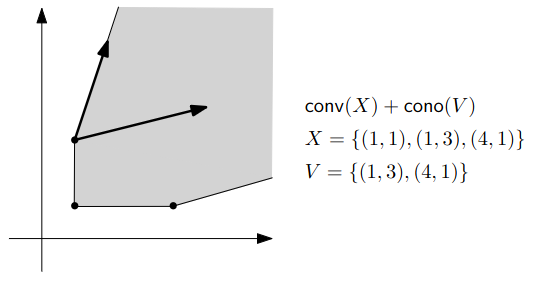
\includegraphics[width=0.5\linewidth]{motzin.png}
\end{center}

\paragraph{Due Rappresentazioni Equivalenti}
Esistono quindi due rappresentazioni per i poliedri:
\begin{enumerate}
    \item Poliedri come intersezioni di semispazi (descrizione \emph{esterna}, per vincoli).
    \item Poliedri come somma di un politopo e di un cono (descrizione \emph{interna}, per punti e direzioni).
\end{enumerate}
Le due rappresentazioni sono equivalenti (grazie al teorema di Motzkin) ma \textbf{non hanno la stessa dimensione}: passare dall'una all'altra può costare un'esplosione esponenziale.
Prendiamo come controesempio il poliedro definito dall'insieme di vincoli $0 \le x_i \le 1$ per $i=1,\dots,n$.
I semispazi coinvolti sono $2n$. I vertici sono invece $2^n$; per rendersene conto basta osservare che i poliedri definiti sono gli ipercubi in $\mathbb{R}^n$ di lato pari a 1 e con un vertice nell'origine. Tali ipercubi hanno effettivamente $2^n$ vertici (uno per ogni scelta, indipendente per ciascuna coordinata, fra $x_i=0$ e $x_i=1$).

\noindent\textit{Conseguenza pratica.} Per $n=30$ la descrizione per vincoli usa 60 disuguaglianze, quella per vertici oltre un miliardo di punti. Ecco perché nessun algoritmo sensato \textbf{enumera} i vertici: il simplesso ne visita pochi, muovendosi lungo gli spigoli verso valori migliori dell'obiettivo.

\subsubsection{Proprietà fondamentale della PL}

\paragraph{Cosa dice, in breve.} È il teorema che chiude il cerchio e giustifica il simplesso. Dice due cose:
\begin{enumerate}
    \item un problema di PL è illimitato \emph{esattamente quando} esiste una direzione di fuga $v_j$ del poliedro lungo la quale l'obiettivo cresce, cioè con $cv_j>0$;
    \item se non è illimitato, allora \textbf{almeno un vertice è ottimo} --- quindi cercare solo fra i vertici è corretto.
\end{enumerate}

\noindent\textbf{Teorema.} Sia $P=\{x \mid Ax \le b\}$ e siano $x_1, \dots, x_s, v_1, \dots, v_t \in \mathbb{R}^n$ tali che:
\[ P = \text{conv}(\{x_1, \dots, x_s\}) + \text{cono}(\{v_1, \dots, v_t\}) \]
Allora il problema $\max\{cx \mid Ax \le b\}$ ha \textbf{ottimo finito} se e solo se $cv_j \le 0$ per ogni $j \in \{1, \dots, t\}$.
In tal caso esiste inoltre un $k \in \{1, \dots, s\}$ tale che $x_k$ è una soluzione ottima.

\noindent\textit{Esempio (il teorema all'opera sui due poliedri di prima).} Con $c=(1,1)$:
\begin{itemize}
    \item Sul problema guida $P$ (Esempio A) non ci sono direzioni ($t=0$): la condizione "$cv_j\le0$ per ogni $j$" è vuota e quindi vera, l'ottimo è finito ed è in un vertice. Basta valutare $c x_i$ sui 5 vertici: il massimo è $c\cdot(3,2)=5$.
    \item Sul poliedro illimitato $P'$ (Esempio B) i raggi estremi sono $v_1=(1,0)$ e $v_2=(0,1)$, e $cv_1 = 1 > 0$: il problema è \textbf{illimitato}. Concretamente, partendo da $(2,0)$ e muovendosi lungo $v_1$ si ottengono i punti $(2+\mu,0)$ con obiettivo $2+\mu \to +\infty$.
    \item Se sullo stesso $P'$ cambiassimo obiettivo in $\min\{x+y\}$, cioè $\max\{-x-y\}$ con $c=(-1,-1)$, allora $cv_1=cv_2=-1\le0$: ottimo finito, da cercare fra i vertici $(2,0)$ e $(0,1)$, che valgono $-2$ e $-1$. Il massimo è $-1$ in $(0,1)$, cioè $\min = 1$.
\end{itemize}

\noindent\textbf{Dimostrazione.}
L'idea è \emph{cambiare variabili}: invece di ottimizzare su $x$, si ottimizza sui coefficienti $\lambda$ e $\mu$ della decomposizione di Motzkin, dove il problema diventa trasparente.

\noindent Per il Teorema di Decomposizione abbiamo che il problema $\max\{cx \mid Ax \le b\}$ è equivalente al seguente problema sulle variabili $\lambda_1, \dots, \lambda_s$ e $\mu_1, \dots, \mu_t$:
\[ \max c \left( \sum_{i=1}^s \lambda_i x_i + \sum_{j=1}^t \mu_j v_j \right) = \max \sum_{i=1}^s \lambda_i (cx_i) + \sum_{j=1}^t \mu_j (cv_j) \]
soggetto a: $\sum_{i=1}^s \lambda_i = 1$; $\lambda_i \ge 0$; $\mu_j \ge 0$.

\noindent Si noti che i $\lambda_i$ sono \emph{vincolati} a sommare a 1 (quindi il loro contributo è limitato), mentre i $\mu_j$ sono liberi di crescere: tutta la questione dell'illimitatezza sta in quel secondo termine. Tale problema ha ottimo finito se e solo se $cv_j \le 0$ per ogni $j \in \{1, \dots, t\}$. Infatti:
\subparagraph{$\implies$} Se fosse $cv_j > 0$ per qualche $j \in \{1, \dots, t\}$, allora si potrebbe pompare $\mu_j$ facendo crescere a piacimento la funzione obiettivo, e il problema sarebbe illimitato.

\subparagraph{$\impliedby$} Supponiamo che $cv_j \le 0$ per ogni $j \in \{1, \dots, t\}$ e prendiamo un $y \in P$. Abbiamo che, se $\lambda_i$ e $\mu_j$ sono i corrispondenti coefficienti del teorema di decomposizione, si ha che $\sum_{j=1}^t \mu_j (cv_j) \le 0$ (somma di termini $\ge0$ moltiplicati per termini $\le0$) e quindi:
\[ cy = \sum_{i=1}^s \lambda_i (cx_i) + \sum_{j=1}^t \mu_j (cv_j) \le \sum_{i=1}^s \lambda_i (cx_i) \]
Se consideriamo il vertice migliore $x_k$, ossia tale per cui $cx_k$ sia massimo, si ha che:
\[ cy \le \sum_{i=1}^s \lambda_i (cx_i) \le \sum_{i=1}^s \lambda_i (cx_k) = cx_k \]
(l'ultima uguaglianza perché $\sum_i \lambda_i = 1$: una media pesata di valori tutti $\le cx_k$ non può superare $cx_k$).
Quindi il valore della soluzione in un qualunque punto $y \in P$ non è migliore del valore della soluzione corrispondente al vertice $x_k$ migliore $\implies x_k$ è una soluzione ottima finita. \hfill$\square$

\subsubsection{Riepilogo della sezione}
\begin{itemize}
    \item Regione ammissibile di un problema di PL $=$ \textbf{poliedro} $\{x \mid Ax\le b\}$, intersezione di $m$ semispazi; è \textbf{convessa}.
    \item Bloccando come uguaglianze un sottoinsieme $I$ di vincoli si ottengono le \textbf{facce}; rango $n \Rightarrow$ vertice, rango $n-1 \Rightarrow$ spigolo.
    \item Un \textbf{vertice} $=$ una \textbf{soluzione di base ammissibile} $x_B = A_B^{-1}b_B$ con $A_B$ quadrata invertibile e $x_B$ che soddisfa tutti gli altri vincoli. È la definizione algebrica, calcolabile, che usa il simplesso.
    \item \textbf{Motzkin}: $P = \text{conv}(X) + \text{cono}(V)$, parte limitata (vertici) $+$ parte illimitata (raggi estremi).
    \item \textbf{Proprietà fondamentale}: $\max\{cx\}$ è illimitato $\iff$ esiste un raggio estremo $v_j$ con $cv_j>0$; altrimenti l'ottimo cade in un vertice.
    \item Quindi lo spazio di ricerca si riduce da infinito a finito ($\le \binom{m}{n}$ basi) --- ma è ancora esponenziale, e per questo serve un algoritmo intelligente: il \textbf{simplesso}, che si sposta di vertice in vertice lungo gli spigoli migliorando l'obiettivo.
\end{itemize}

\subsection{Dualità, Direzioni Ammissibili e di Crescita}

\subsubsection{Perché la Dualità?}
La teoria della dualità è una branca dell'algebra lineare estremamente utile nella costruzione di algoritmi per la Programmazione Lineare. Essa si basa sulla definizione di un'\textbf{involuzione} (una funzione inversa di sé stessa) che mappa ogni problema di PL nel suo problema \textbf{duale}. 

In sintesi, ad ogni problema di massimizzazione (Primale) corrisponde un problema di minimizzazione (Duale) strettamente correlato.

\paragraph{L'idea in una riga: il duale è ``la migliore garanzia''}
Immaginiamo di avere un primale di massimo e di aver trovato una soluzione ammissibile che vale $2200$. Abbiamo un \textbf{limite inferiore}: l'ottimo vale almeno $2200$. Ma non sappiamo se possiamo fare meglio. Per esserne certi ci serve un \textbf{limite superiore}: una frase del tipo ``qualunque soluzione ammissibile non può valere più di $K$''.

Il duale è esattamente la macchina che produce quei limiti superiori, e il suo obiettivo è produrre il \textbf{più stretto possibile}. Da dove nascono? Da \textbf{combinazioni dei vincoli}. Prendiamo dei moltiplicatori $y_i \ge 0$, uno per vincolo, e sommiamo i vincoli $A_i x \le b_i$ pesati con $y_i$:
\[
\underbrace{(yA)x}_{\text{combinazione dei membri sinistri}} \;\le\; \underbrace{yb}_{\text{numero noto}}
\]
Se scegliamo i pesi in modo che la combinazione dei membri sinistri \emph{sia proprio} la funzione obiettivo, cioè $yA = c$, allora otteniamo gratis
\[
cx \le yb \qquad \text{per \emph{ogni} } x \text{ ammissibile.}
\]
Il numero $yb$ è quindi un limite superiore valido. Cercare il limite \emph{migliore} significa risolvere $\min\{yb \mid yA = c,\ y\ge 0\}$: ed ecco il duale, che non è caduto dal cielo ma è la formalizzazione di ``trova la combinazione di vincoli che dà la garanzia più stretta''.

\begin{center}
\begin{tikzpicture}[>=latex,scale=1.0]
  \draw[->] (-0.3,0)--(9.6,0);
  \foreach \x in {0,...,9} \draw (\x,0.08)--(\x,-0.08);
  % zone
  \fill[blue!12] (0,0.15) rectangle (4,0.75);
  \fill[red!12]  (5,0.15) rectangle (9.4,0.75);
  \node[font=\small,blue!60!black] at (2,0.45) {valori del primale $cx$};
  \node[font=\small,red!60!black] at (7.2,0.45) {valori del duale $yb$};
  \draw[<-,blue!70!black,thick] (0.2,-0.55)--(4,-0.55);
  \node[font=\scriptsize,blue!60!black,below] at (2.1,-0.6) {si spinge verso destra (max)};
  \draw[<-,red!70!black,thick] (9.3,-0.55)--(5,-0.55);
  \node[font=\scriptsize,red!60!black,below] at (7.2,-0.6) {si spinge verso sinistra (min)};
  \draw[dashed,gray] (4,-0.2)--(4,1.3);
  \draw[dashed,gray] (5,-0.2)--(5,1.3);
  \node[font=\scriptsize,gray!60!black,above left] at (3.9,1.25) {ottimo primale};
  \node[font=\scriptsize,gray!60!black,above right] at (5.1,1.25) {ottimo duale};
  \draw[<->,thick] (4,1.05)--(5,1.05);
  \node[font=\scriptsize,above] at (4.5,1.0) {};
\end{tikzpicture}
\end{center}
\noindent Ogni soluzione primale ammissibile sta a sinistra, ogni soluzione duale ammissibile sta a destra: \emph{nessuna delle due può scavalcare l'altra} (dualità debole). Nella PL i due valori ottimi \textbf{coincidono} (dualità forte): il gap in figura si chiude. Perciò se troviamo una coppia $\bar{x},\bar{y}$ ammissibili con lo stesso valore, abbiamo la \textbf{prova} che entrambe sono ottime, senza dover esplorare altro.

\subsubsection{Primale e Duale: Formulazioni}
Il Primale e il Duale sono costruiti utilizzando i medesimi coefficienti, ma trasposti. Esistono due tipologie principali di coppie:

\paragraph{Coppie Asimmetriche}
\begin{itemize}
    \item \textbf{Primale}: $\max \{cx \mid Ax \le b\}$
    \item \textbf{Duale}: $\min \{yb \mid yA = c, y \ge 0\}$
\end{itemize}

\paragraph{Coppie Simmetriche}
\begin{itemize}
    \item \textbf{Primale}: $\max \{cx \mid Ax \le b, x \ge 0\}$
    \item \textbf{Duale}: $\min \{yb \mid yA \ge c, y \ge 0\}$
\end{itemize}

\paragraph{Tabella di conversione Primale-Duale}
Nel caso generale (vincoli di verso misto e variabili non tutte vincolate in segno) la costruzione del duale segue una tabella di conversione: la funzione obiettivo e i termini noti si scambiano ($c \leftrightarrow b$), ogni \textbf{vincolo} del primale genera una \textbf{variabile} del duale e ogni \textbf{variabile} del primale genera un \textbf{vincolo} del duale.
\begin{center}
\begin{tabular}{lll}
\hline
 & \textbf{max} (primale) & \textbf{min} (duale) \\
\hline
funzione obiettivo & $c$ & $b$ \\
termini noti & $b$ & $c$ \\
\hline
\multirow{3}{*}{vincoli $\to$ variabili} & $A_i x \le b_i$ & $y_i \ge 0$ \\
 & $A_i x \ge b_i$ & $y_i \le 0$ \\
 & $A_i x = b_i$ & $y_i$ libera \\
\hline
\multirow{3}{*}{variabili $\to$ vincoli} & $x_j \ge 0$ & $yA_j \ge c_j$ \\
 & $x_j \le 0$ & $yA_j \le c_j$ \\
 & $x_j$ libera & $yA_j = c_j$ \\
\hline
\end{tabular}
\end{center}
La regola mnemonica è che i vincoli "concordi" col verso dell'ottimizzazione danno variabili non negative, i vincoli di uguaglianza danno variabili libere e, simmetricamente, le variabili libere danno vincoli di uguaglianza.

\paragraph{Ricetta pratica (scrivere il duale in sede d'esame)}
La richiesta "si scriva il duale del problema" vale 2 punti e si svolge in tre mosse:
\begin{enumerate}
    \item \textbf{portare il primale in forma omogenea}: se è di massimo, tutti i vincoli in forma $\le$ (moltiplicando per $-1$ quelli $\ge$ e sdoppiando le uguaglianze); questo evita di dover ragionare sui segni delle variabili duali;
    \item \textbf{trasporre}: la funzione obiettivo del duale è $\min yb$ con i termini noti del primale come coefficienti, e ogni \textit{colonna} $A_j$ di $A$ diventa un vincolo;
    \item \textbf{fissare i domini}: con il primale $\max\{cx \mid Ax\le b\}$ e $x$ libera si ottiene la coppia asimmetrica, quindi vincoli duali di \textbf{uguaglianza} $yA_j = c_j$ e $y \ge 0$; se invece nel primale $x \ge 0$ si ottiene la coppia simmetrica, con vincoli duali $yA_j \ge c_j$.
\end{enumerate}
Errore tipico: dimenticare che se le variabili primali sono \textbf{libere} (come nei tipici esercizi in cui il testo non impone $x \ge 0$) i vincoli duali sono equazioni, non disuguaglianze.

\subsubsection{Esempio: Problema della Dieta}
Consideriamo un allevamento che deve miscelare due mangimi ($A, B$) per soddisfare i requisiti minimi di carboidrati, proteine e vitamine al minor costo possibile.

\begin{figure}[h!]
    \centering
    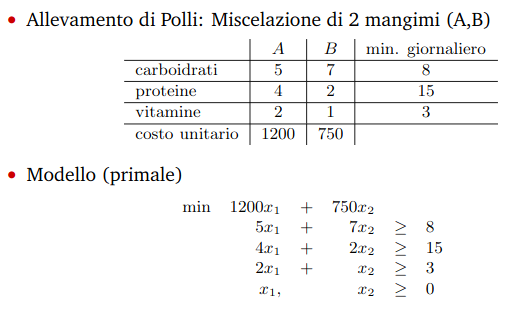
\includegraphics[width=0.5\linewidth]{dieta.png}
\end{figure}

\noindent Il modello \textbf{Primale} (minimizzazione dei costi) si presenta come:
\[
\begin{aligned}
\min \quad & 1200x_1 + 750x_2 \\
\text{s.t.} \quad & 5x_1 + 7x_2 \ge 8 \quad \text{(Carboidrati)} \\
& 4x_1 + 2x_2 \ge 15 \quad \text{(Proteine)} \\
& 2x_1 + x_2 \ge 3 \quad \text{(Vitamine)} \\
& x_1, x_2 \ge 0
\end{aligned}
\]

\noindent Il punto di vista \textbf{Duale} è quello di un produttore di pillole di sostanze nutritive che vuole massimizzare il prezzo di vendita delle pillole, rimanendo però competitivo rispetto ai mangimi:
\[
\begin{aligned}
\max \quad & 8y_1 + 15y_2 + 3y_3 \\
\text{s.t.} \quad & 5y_1 + 4y_2 + 2y_3 \le 1200 \\
& 7y_1 + 2y_2 + y_3 \le 750 \\
& y_1, y_2, y_3 \ge 0
\end{aligned}
\]

Si può osservare che il ricavo del venditore di pillole sarà sempre inferiore o uguale al costo di qualunque miscelazione ammissibile di mangimi (relazione di dualità debole).

\begin{figure}[h!]
    \centering
    \begin{minipage}{0.3\linewidth}
        \centering
        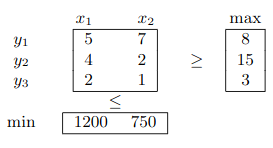
\includegraphics[width=\linewidth]{relazioneP-D.png}
    \end{minipage}
    \hfill
    \begin{minipage}{0.6\linewidth}
        \centering
        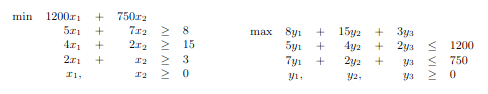
\includegraphics[width=\linewidth]{relazioneP-D2.png}
    \end{minipage}
\end{figure}

\noindent Moltiplicando i vincoli del duale per $x_1,x_2$ e sommandoli:
\begin{align*}
    x_1(5y_1+4y_2+2y_3)+x_2(7y_1+2y_2+y_3)&\le 1200x_1+750x_2\\
    y_1(5x_1+7x_2)+y_2(4x_1+2x_2)+y_3(2x_1+x_2) &\le 1200x_1+750x_2
\end{align*}
In qualunque dieta ammissibile si ha $5x_1+7x_2 \ge 8$
\[
8y_1+15y_2+3y_3 \le 1200x_1+750x_2
\]

\subsubsection{Esempio: Problema dei Trasporti}
Un produttore ha $n$ fabbriche e $m$ depositi. Deve trasportare i prodotti dalle fabbriche (con produzione $a_i$) ai depositi (con capacità $b_j$) a costo minimo.

\begin{itemize}
    \item $a_i$ quantità prodotto dalla fabbrica $i$ ($i=1..n$)
    \item $b_j$ capacità del deposito $j$ ($j=1..m$)
    \item supponiamo $\sum_{i=1}^n a_i = \sum_{j=1}^m b_j$
    \item $c_{ij}$ costo unitario di trasporto da fabbrica $i$ a deposito $j$
\end{itemize}
L'obiettivo è trasportare il prodotto dalle fabbriche ai depositi a costo minimo
\begin{itemize}
    \item $x_{ij}$ quantità di prodotto inviato da \textit{i} a \textit{j}
\end{itemize}

\paragraph{Modello Primale}
\[
\begin{aligned}
\min \quad & \sum_{i=1}^n \sum_{j=1}^m c_{ij}x_{ij} \\
\text{s.t.} \quad & \sum_{j=1}^m x_{ij} = a_i \quad \forall i=1..n \\
& \sum_{i=1}^n x_{ij} = b_j \quad \forall j=1..m \\
& x_{ij} \ge 0
\end{aligned}
\]

\paragraph{Modello Duale}
Un'azienda di trasporti compra il prodotto alla fabbrica $i$ (prezzo $\lambda_i$) e lo rivende al deposito $j$ (prezzo $\mu_j$), massimizzando il guadagno netto e rimanendo competitiva rispetto ai costi di trasporto propri del produttore:
\[
\begin{aligned}
\max \quad & -\sum_{i=1}^n a_i \lambda_i + \sum_{j=1}^m b_j \mu_j \\
\text{s.t.} \quad & -\lambda_i + \mu_j \le c_{ij} \quad i=1..n,j=1..m
\end{aligned}
\]

\begin{figure}[h!]
    \centering
    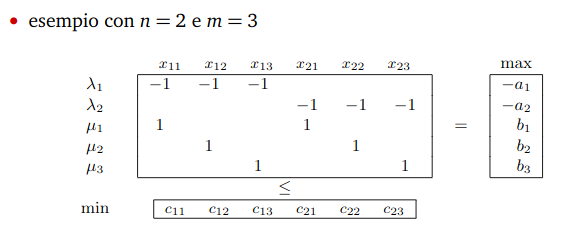
\includegraphics[width=0.5\linewidth]{probl_trasp.png}
\end{figure}

\subsubsection{Proprietà della Dualità}

\paragraph{Dualità dell'Involuzione}
Il duale del duale coincide con il primale. Ad esempio, per una coppia simmetrica, trasformando il duale in un problema di massimo e applicando nuovamente le regole di transposizione, si ritorna alla forma del primale originale.

\paragraph{Teorema Debole di Dualità}
Siano $\bar{x}$ una soluzione ammissibile per il primale e $\bar{y}$ una soluzione ammissibile per il duale. Allora vale sempre:
\[ c\bar{x} \le \bar{y}b \]

\noindent \textbf{Dimostrazione (caso asimmetrico):}
Sapendo che $A\bar{x} \le b$ e $\bar{y} \ge 0$, moltiplicando si ottiene $\bar{y}A\bar{x} \le \bar{y}b$. Poiché nel duale vale $\bar{y}A = c$, allora $c\bar{x} \le \bar{y}b$.

\paragraph{Corollari del Teorema Debole}
\begin{enumerate}
    \item Se il primale è illimitato, allora il duale è impossibile (vuoto).
    \item Se $\bar{x}$ e $\bar{y}$ sono soluzioni ammissibili e $c\bar{x} = \bar{y}b$, allora $\bar{x}$ e $\bar{y}$ sono soluzioni \textbf{ottime} per i rispettivi problemi.
\end{enumerate}

\subsubsection{Esempio: Produzione Microprocessori}
Riprendiamo l'esempio della produzione di microprocessori per verificare l'ottimalità tramite la dualità.

\paragraph{Primale}
\[
\begin{aligned}
\max \quad & 500x_1 + 200x_2 \\
\text{s.t.} \quad & x_1 \le 4 \\
& x_2 \le 7 \\
& 2x_1 + x_2 \le 9 \\
& x_1, x_2 \ge 0
\end{aligned}
\]

\begin{center}
    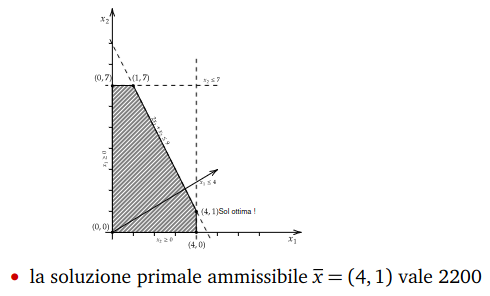
\includegraphics[width=0.5\linewidth]{processori2.png}
\end{center}

\paragraph{Duale}
\[
\begin{aligned}
\min \quad & 4y_1 + 7y_2 + 9y_3 \\
& y_1 + 2y_3 - y_4 = 500 \\
& y_2 + y_3 - y_5 = 200 \\
& y_1, y_2, y_3, y_4, y_5 \ge 0
\end{aligned}
\]

\noindent È facile verificare che la soluzione duale $\bar{y} = (100, 0, 200, 0, 0, 0)$ è ammissibile e vale 2200 per cui la soluzione $\bar{x} = (4, 1)$ è ottima!

\paragraph{Perché questa è una \emph{prova} e non un controllo a campione}
Facciamo le verifiche una per una, perché è esattamente ciò che va saputo fare all'esame.
\begin{enumerate}
    \item \textbf{$\bar{x}=(4,1)$ è ammissibile}: $4 \le 4$ \checkmark, $1 \le 7$ \checkmark, $2(4)+1 = 9 \le 9$ \checkmark, $x \ge 0$ \checkmark. Vale $500(4)+200(1) = 2200$.
    \item \textbf{$\bar{y}$ è ammissibile}: tutte le componenti sono $\ge 0$ \checkmark; primo vincolo $y_1 + 2y_3 - y_4 = 100 + 400 - 0 = 500$ \checkmark; secondo $y_2 + y_3 - y_5 = 0 + 200 - 0 = 200$ \checkmark. Vale $4(100)+7(0)+9(200) = 400 + 1800 = 2200$.
    \item \textbf{I due valori coincidono} ($2200 = 2200$) $\Rightarrow$ per il corollario del teorema debole, \emph{entrambe} sono ottime.
\end{enumerate}
Il punto concettuale: la dualità debole dice che \emph{nessuna} soluzione primale può superare $2200$ (perché $\bar{y}$ ne è testimone) e che \emph{nessuna} soluzione duale può scendere sotto $2200$ (perché $\bar{x}$ ne è testimone). Le due si incastrano e non lasciano spazio: non serve esaminare gli altri vertici. Questa coppia $(\bar{x},\bar{y})$ si chiama \textbf{certificato di ottimalità}, ed è facilissima da controllare anche per chi non ha idea di come sia stata trovata.

\noindent Osserviamo infine che $\bar{y}_2 = 0$: il vincolo $x_2 \le 7$ è \emph{lasco} in $\bar{x}$ ($x_2 = 1 < 7$), quindi il suo peso nella combinazione è nullo. È lo stesso fenomeno visto con i vincoli attivi: ciò che non ci sta stringendo non serve a certificare nulla.

\subsubsection{Direzioni Ammissibili e di Crescita}

\paragraph{L'idea di fondo}
Fin qui abbiamo guardato il problema ``da fuori'' (dove sta l'ottimo nel poliedro). Adesso lo guardiamo \textbf{da dentro}, mettendoci in piedi su una soluzione ammissibile $\bar{x}$ e chiedendoci una cosa sola:
\begin{center}
\emph{da qui, in quali direzioni posso muovermi senza uscire dalla regione ammissibile, e fra queste ce n'è una che mi fa guadagnare?}
\end{center}
Se la risposta è sì, $\bar{x}$ non è ottima e sappiamo anche \emph{dove andare}. Se la risposta è no, $\bar{x}$ è ottima. Tutto il Simplesso è questa domanda ripetuta di vertice in vertice.

Conviene tenere separate le due metà della domanda, perché dipendono da cose diverse:
\begin{center}
\begin{tabular}{lll}
\hline
 & \textbf{Ammissibile?} & \textbf{Di crescita?} \\
\hline
significato & ``non esco dal poliedro'' & ``la funzione obiettivo sale'' \\
dipende da & vincoli \emph{attivi} in $\bar{x}$ & solo dal vettore $c$ \\
condizione & $A_{I(\bar{x})}\,\xi \le 0$ & $c\,\xi > 0$ \\
cambia da punto a punto? & \textbf{sì} & \textbf{no} \\
\hline
\end{tabular}
\end{center}

\paragraph{Direzioni Ammissibili}
Data una coppia asimmetricamente definita di problemi (Primale e Duale), consideriamo una soluzione ammissibile $\bar{x}$ per il primale. L'obiettivo è determinare se, spostandoci lungo una direzione specifica dello spazio a partire da $\bar{x}$, si rimanga all'interno della regione ammissibile.

Un vettore $\xi \in \mathbb{R}^n$ è definito \textbf{Direzione Ammissibile} se esiste un valore $\bar{\lambda} > 0$ tale che il punto $x(\lambda) = \bar{x} + \lambda \xi$ risulti ammissibile nel primale per ogni $\lambda \in [0, \bar{\lambda}]$.

\noindent In parole povere: $\xi$ è la \emph{freccia} che indica dove puntare, $\lambda$ è \emph{quanto} camminiamo lungo la freccia, e $x(\lambda)$ è il punto in cui arriviamo. La direzione è ammissibile se esiste almeno un passetto iniziale (per piccolo che sia) che ci mantiene dentro. Attenzione a due punti che confondono spesso:
\begin{itemize}
    \item la richiesta è \textbf{locale}: basta che un tratto iniziale $[0,\bar{\lambda}]$ resti dentro, non serve che si resti dentro per sempre;
    \item la lunghezza di $\xi$ è irrilevante: $\xi$ e $2\xi$ sono la stessa direzione (cambia solo la scala di $\lambda$). Per questo l'insieme delle direzioni ammissibili sarà un \textbf{cono}.
\end{itemize}

\begin{center}
\begin{tikzpicture}[>=latex,scale=1.25]
  \fill[blue!12] (0,0)--(3,0)--(3,1.6)--(1.6,2.6)--(0,2)--cycle;
  \draw[blue!70!black,thick] (0,0)--(3,0)--(3,1.6)--(1.6,2.6)--(0,2)--cycle;
  \node[font=\small,blue!50!black] at (1.0,0.75) {$P$};
  % punto sul bordo
  \fill (3,0.8) circle (1.6pt);
  \node[font=\small,right] at (3.05,0.75) {$\bar{x}$};
  \node[font=\scriptsize,rotate=90,above] at (3.0,0.15) {vincolo attivo};
  % direzione ammissibile
  \draw[->,green!50!black,very thick] (3,0.8)--(1.7,1.3);
  \node[font=\scriptsize,green!35!black,above left] at (1.9,1.28) {$\xi_1$ ammissibile};
  % direzione ammissibile tangente
  \draw[->,green!50!black,very thick] (3,0.8)--(3,1.5);
  \node[font=\scriptsize,green!35!black,right] at (3.02,1.35) {$\xi_2$ ammissibile (scivola sul bordo)};
  % direzione non ammissibile
  \draw[->,red,very thick] (3,0.8)--(3.9,0.95);
  \node[font=\scriptsize,red,right] at (3.9,0.98) {$\xi_3$ NON ammissibile};
  \draw[->] (-0.3,0)--(-0.3,2.8) node[above,font=\scriptsize]{$x_2$};
  \draw[->] (-0.3,-0.25)--(4.6,-0.25) node[right,font=\scriptsize]{$x_1$};
\end{tikzpicture}
\end{center}
\noindent Da $\bar{x}$, che sta sul bordo destro, $\xi_1$ rientra nel poliedro e $\xi_2$ scorre lungo il bordo: entrambe ammissibili. $\xi_3$ punta verso l'esterno del vincolo attivo: già per $\lambda$ arbitrariamente piccolo si esce, quindi non è ammissibile.

\paragraph{Perché contano solo i vincoli attivi}
Questo è il punto che rende il tutto calcolabile. Un vincolo $A_i x \le b_i$ in $\bar{x}$ può trovarsi in due stati:
\begin{itemize}
    \item \textbf{attivo} (o \emph{stretto}): $A_i\bar{x} = b_i$, siamo appoggiati contro il muro. Qualunque movimento che punti anche solo un po' ``verso fuori'' lo viola immediatamente: dobbiamo imporre $A_i\xi \le 0$;
    \item \textbf{non attivo} (\emph{lasco}): $A_i\bar{x} < b_i$, c'è dello spazio libero prima del muro. Un passo abbastanza piccolo non riesce a consumarlo, qualunque sia la direzione: nessuna condizione da imporre.
\end{itemize}
Ecco perché nel lemma compare solo la sottomatrice $A_{I(\bar{x})}$ e non tutta $A$: i vincoli lontani non vincolano la partenza.

\begin{figure}[h!]
    \centering
    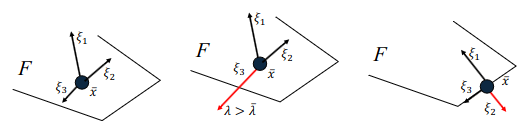
\includegraphics[width=0.5\linewidth]{direzAmmiss.png}
\end{figure}

\paragraph{Lemma delle Direzioni Ammissibili}
Il vettore $\xi$ è una direzione ammissibile per il punto $\bar{x}$ se e solo se $A_{I(\bar{x})} \xi \le 0$, dove $I(\bar{x})$ rappresenta l'insieme degli indici dei vincoli attivi in $\bar{x}$.

\textit{Dimostrazione (Sintesi):}
Affinché $\xi$ sia ammissibile, per ogni vincolo $i \in \{1, \dots, m\}$ deve valere $A_i x(\lambda) = A_i \bar{x} + \lambda A_i \xi \le b_i$. 
\begin{itemize}
    \item Se il vincolo $i$ è attivo ($i \in I(\bar{x})$), allora $A_i \bar{x} = b_i$. La condizione si riduce a $\lambda A_i \xi \le 0$, che per $\lambda > 0$ implica $A_i \xi \le 0$.
    \item Se il vincolo $i$ non è attivo ($i \notin I(\bar{x})$), allora $A_i \bar{x} < b_i$. In questo caso, per un $\lambda$ sufficientemente piccolo, la disequazione rimane soddisfatta indipendentemente dal valore di $\xi$.
\end{itemize}

\paragraph{Cono delle Direzioni Ammissibili}
L'insieme di tutte le direzioni ammissibili per $\bar{x}$ definisce un \textbf{cono poliedrico} espresso come:
\[ C(\bar{x}) = \{ \xi \in \mathbb{R}^n : A_{I(\bar{x})} \xi \le 0 \} \]
È importante notare che se $\bar{x}$ è un punto interno (nessun vincolo attivo), allora $C(\bar{x}) = \mathbb{R}^n$, ovvero ogni direzione è localmente ammissibile.

\noindent Si chiama \textbf{cono} perché è chiuso rispetto alle combinazioni non negative: se $\xi$ è ammissibile lo è anche $2\xi$ o $0.1\,\xi$ (stessa freccia, lunghezza diversa), e se $\xi^1,\xi^2$ lo sono lo è anche $\xi^1+\xi^2$. Graficamente è uno ``spicchio'' con il vertice nell'origine. La sua ampiezza racconta quanto siamo bloccati:
\begin{center}
\begin{tabular}{lll}
\hline
\textbf{dove si trova $\bar{x}$} & \textbf{vincoli attivi} & \textbf{cono $C(\bar{x})$} \\
\hline
interno al poliedro & nessuno & tutto $\mathbb{R}^n$: libertà totale \\
su una faccia (bordo) & $1$ & un semipiano \\
in un vertice (in $\mathbb{R}^2$) & $2$ & uno spicchio stretto \\
\hline
\end{tabular}
\end{center}

\paragraph{Esempio numerico del cono}
Prendiamo il poliedro
\[
x_1 \le 4, \qquad x_2 \le 7, \qquad 2x_1 + x_2 \le 9, \qquad -x_1 \le 0, \qquad -x_2 \le 0
\]
e il vertice $\bar{x} = (4,1)$. Verifichiamo quali vincoli sono attivi:
\begin{center}
\begin{tabular}{lccc}
\hline
vincolo & $A_i\bar{x}$ & $b_i$ & stato \\
\hline
$x_1 \le 4$ & $4$ & $4$ & \textbf{attivo} \\
$x_2 \le 7$ & $1$ & $7$ & lasco \\
$2x_1+x_2 \le 9$ & $9$ & $9$ & \textbf{attivo} \\
$-x_1 \le 0$ & $-4$ & $0$ & lasco \\
$-x_2 \le 0$ & $-1$ & $0$ & lasco \\
\hline
\end{tabular}
\end{center}
Dunque $I(\bar{x}) = \{1,3\}$ e il cono è definito da due sole disuguaglianze:
\[
C(\bar{x}) = \left\{ \xi \in \mathbb{R}^2 \;\middle|\; \xi_1 \le 0, \;\; 2\xi_1 + \xi_2 \le 0 \right\}
\]
Proviamo tre direzioni:
\begin{itemize}
    \item $\xi = (-1,0)$: $\xi_1 = -1 \le 0$ e $2(-1)+0 = -2 \le 0$ $\Rightarrow$ \textbf{ammissibile} (torniamo indietro lungo $x_1$);
    \item $\xi = (-1,2)$: $-1 \le 0$ e $-2+2 = 0 \le 0$ $\Rightarrow$ \textbf{ammissibile}, e scorre \emph{esattamente lungo} il vincolo $2x_1+x_2 = 9$ (spigolo del poliedro);
    \item $\xi = (0,1)$: $\xi_1 = 0 \le 0$ ok, ma $2(0)+1 = 1 > 0$ $\Rightarrow$ \textbf{non ammissibile}: salire in verticale viola subito $2x_1+x_2\le 9$.
\end{itemize}

\begin{center}
\begin{tikzpicture}[>=latex,scale=0.78]
  % poliedro: (0,0),(4,0),(4,1),(1,7),(0,7)
  \fill[blue!12] (0,0)--(4,0)--(4,1)--(1,7)--(0,7)--cycle;
  \draw[blue!70!black,thick] (0,0)--(4,0)--(4,1)--(1,7)--(0,7)--cycle;
  \draw[->] (-0.5,0)--(6.5,0) node[right,font=\small]{$x_1$};
  \draw[->] (0,-0.5)--(0,8.2) node[above,font=\small]{$x_2$};
  \foreach \x in {1,2,3,4,5} \draw (\x,0.1)--(\x,-0.1) node[below,font=\tiny]{\x};
  \foreach \y in {1,3,5,7} \draw (0.1,\y)--(-0.1,\y) node[left,font=\tiny]{\y};
  \node[font=\small,blue!50!black] at (1.4,2.2) {$P$};
  % cono traslato in (4,1)
  \fill[green!25,opacity=0.6] (4,-0.4)--(4,1)--(2.0,5.0)--(-0.5,5.0)--(-0.5,-0.4)--cycle;
  \fill (4,1) circle (2.2pt);
  \node[font=\small,right] at (4.9,1.9) {$\bar{x}=(4,1)$};
  \draw[gray] (4.85,1.85)--(4.1,1.1);
  \draw[->,green!45!black,very thick] (4,1)--(2.6,1) node[below,font=\scriptsize]{$\xi=(-1,0)$};
  \draw[->,green!45!black,very thick] (4,1)--(2.6,3.8) node[above right,font=\scriptsize]{$\xi=(-1,2)$};
  \draw[->,red,very thick] (4,1)--(4,2.6) node[right,font=\scriptsize]{$\xi=(0,1)$ esce};
  \node[font=\scriptsize,green!35!black] at (0.8,4.4) {$C(\bar{x})$ traslato in $\bar{x}$};
  % rette attive
  \draw[dashed,gray] (4,-0.3)--(4,7.6) node[above,font=\tiny,black]{$x_1=4$};
  \draw[dashed,gray] (-0.2,9.4)--(4.7,-0.4);
  \node[font=\tiny,rotate=-52] at (2.35,5.6) {$2x_1{+}x_2=9$};
\end{tikzpicture}
\end{center}
\noindent Il cono (in verde) è \emph{lo stesso spicchio} del poliedro visto da vicino a partire da $\bar{x}$: è la ``vista locale'' del poliedro, con i vincoli laschi cancellati e il vertice portato nell'origine.

\begin{figure}[h!]
    \begin{minipage}{0.25\linewidth}
        \centering
        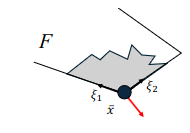
\includegraphics[width=\linewidth]{direzAmm1.png}
    \end{minipage}
    \hfill
    \begin{minipage}{0.25\linewidth}
        \centering
        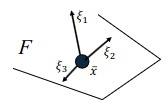
\includegraphics[width=\linewidth]{direzAmm2.png}
    \end{minipage}
\end{figure}

\paragraph{Direzioni di Crescita}
Una direzione $\xi \in \mathbb{R}^n$ è detta \textbf{direzione di crescita} per $\bar{x}$ se uno spostamento lungo di essa incrementa il valore della funzione obiettivo. Ciò accade se:
\[ c x(\lambda) = c \bar{x} + \lambda c \xi > c \bar{x} \iff c \xi > 0 \]
A differenza dell'ammissibilità, la proprietà di essere una direzione di crescita dipende unicamente dal vettore dei costi $c$ e non dal punto specifico $\bar{x}$.

\noindent Geometricamente $c\xi > 0$ significa che $\xi$ forma un \textbf{angolo acuto} con il vettore $c$ (ricordiamo: $c\xi = \|c\|\|\xi\|\cos\theta$, quindi il segno è quello del coseno). Il vettore $c$ è la direzione di massima pendenza in salita della funzione obiettivo, e le curve di livello $cx = \text{cost.}$ sono le rette perpendicolari a $c$: muoversi ``in avanti'' rispetto a esse fa salire, muoversi ``all'indietro'' fa scendere, muoversi lungo di esse lascia il valore invariato ($c\xi = 0$, direzione \emph{neutra}).

\begin{center}
\begin{tikzpicture}[>=latex,scale=1.15]
  \clip (-2.8,-2.4) rectangle (3.4,2.6);
  % semipiano di crescita: lato di c rispetto alla retta perpendicolare a c
  \fill[green!15] (-1.8,2.4)--(3.4,-1.5)--(3.4,2.6)--(-1.8,2.6)--cycle;
  % curve di livello (perpendicolari a c, direzione (-0.6,0.8))
  \foreach \k in {-2,-1,0,1,2}
    \draw[gray!45] ({0.8*\k-1.8},{0.6*\k+2.4}) -- ({0.8*\k+2.2},{0.6*\k-2.266});
  % retta c xi = 0
  \draw[dashed,gray!80,thick] (-1.8,2.4)--(2.2,-2.266);
  \node[font=\scriptsize,gray!45!black,rotate=-49] at (-1.15,2.1) {$c\xi=0$ (neutra)};
  \draw[->,very thick,black] (0,0)--(1.6,1.2) node[right,font=\small]{$c$};
  \draw[->,green!50!black,very thick] (0,0)--(0.4,1.9);
  \node[font=\scriptsize,green!35!black,above] at (0.35,1.9) {$c\xi>0$: cresce};
  \draw[->,red,very thick] (0,0)--(-1.7,-0.6);
  \node[font=\scriptsize,red,below] at (-1.5,-0.7) {$c\xi<0$: cala};
  \draw[->,gray!55!black,very thick] (0,0)--(-1.05,1.4);
  \node[font=\scriptsize,gray!45!black,left] at (-1.05,1.45) {$c\xi=0$};
  \fill (0,0) circle (2pt);
  \node[font=\small,below right] at (0.05,-0.1) {$\bar{x}$};
  \node[font=\scriptsize,gray!60!black,rotate=-49] at (2.75,1.0) {curve di livello};
\end{tikzpicture}
\end{center}
\noindent \textbf{Nota chiave}: questo disegno non cambia mai al variare di $\bar{x}$ (il semipiano verde si trasla e basta), mentre il cono delle direzioni ammissibili cambia a ogni punto. È per questo che l'ottimalità si legge come \emph{intersezione} fra un oggetto fisso (il semipiano di crescita) e uno variabile (il cono).

\paragraph{Direzioni di Crescita e Ottimalità}
Le due nozioni si combinano in un criterio esatto di ottimalità. Anzitutto due osservazioni:
\begin{itemize}
    \item se $c = 0$ la funzione obiettivo vale sempre $0$ e ogni soluzione ammissibile è ottima;
    \item se $c \ne 0$ e in $\bar{x}$ esiste una direzione ammissibile che sia anche di crescita, allora $\bar{x}$ non può essere ottima.
\end{itemize}

\noindent\textbf{Lemma.} Sia $c \ne 0$. Una soluzione ammissibile $\bar{x}$ è ottima per $(P)$ \textbf{se e solo se} $\bar{x}$ non ammette direzioni ammissibili che siano anche di crescita.

\noindent\textbf{Dimostrazione.}
\begin{itemize}
    \item[$\implies$] Se $\bar{x}$ è ottima non possono esistere direzioni ammissibili di crescita, altrimenti spostandosi lungo di esse si troverebbe una soluzione ammissibile migliore.
    \item[$\impliedby$] Supponiamo che $\bar{x}$ non sia ottima: esiste allora $x'$ ammissibile con $cx' > c\bar{x}$, cioè $c(x'-\bar{x}) > 0$. La direzione $\xi = x' - \bar{x}$ è di crescita (perché $c\xi > 0$) ed è anche ammissibile, poiché $x'$ e $\bar{x}$ appartengono al poliedro $P$, che è convesso e quindi contiene tutto il segmento che li congiunge. Abbiamo costruito una direzione ammissibile di crescita, contro l'ipotesi.
\end{itemize}
Questo lemma è il cuore del criterio di arresto del Simplesso: verificare l'ottimalità di un vertice equivale a verificare che da esso non parta alcuna direzione ammissibile di crescita.

\paragraph{Il criterio letto sul disegno}
Sovrapponiamo i due oggetti: il \textbf{cono} $C(\bar{x})$ (verde, cambia con il punto) e il \textbf{semipiano di crescita} $\{\xi : c\xi > 0\}$ (grigio, sempre lo stesso). Solo l'intersezione conta:
\begin{center}
\begin{tikzpicture}[>=latex,scale=0.95]
% ---- pannello sinistro: NON ottima ----
\begin{scope}
  \fill[gray!20] (-2.2,0) rectangle (2.2,2.4);
  \node[font=\scriptsize,gray!55!black] at (1.65,2.15) {$c\xi>0$};
  \draw[dashed,gray!70] (-2.2,0)--(2.2,0);
  % cono: raggi (1,-0.5) e (-0.7,1.4)
  \fill[green!30,opacity=0.8] (0,0)--(2.0,-1.0)--(2.0,-1.6)--(-1.6,-1.6)--(-1.6,3.2)--(-1.05,2.1)--cycle;
  \begin{scope}
    \clip (-2.2,0) rectangle (2.2,2.4);
    \fill[orange!75,opacity=0.9] (0,0)--(2.0,-1.0)--(2.0,-1.6)--(-1.6,-1.6)--(-1.6,3.2)--(-1.05,2.1)--cycle;
  \end{scope}
  \draw[->,thick] (0,0)--(0,1.9) node[above,font=\scriptsize]{$c$};
  \fill (0,0) circle (1.8pt);
  \node[font=\scriptsize,below right] at (0.05,-0.05) {$\bar{x}$};
  \node[font=\scriptsize,green!30!black] at (-1.0,-1.15) {$C(\bar{x})$};
  \node[font=\scriptsize,orange!65!black] at (-1.15,1.35) {intersezione $\ne\emptyset$};
  \node[font=\small,align=center] at (0,-2.3) {\textbf{NON ottima}\\ esiste dove andare};
\end{scope}
% ---- pannello destro: ottima ----
\begin{scope}[xshift=7.0cm]
  \fill[gray!20] (-2.2,0) rectangle (2.2,2.4);
  \node[font=\scriptsize,gray!55!black] at (1.65,2.15) {$c\xi>0$};
  \draw[dashed,gray!70] (-2.2,0)--(2.2,0);
  \fill[green!30,opacity=0.8] (0,0)--(1.7,-1.6)--(-1.7,-1.6)--cycle;
  \draw[->,thick] (0,0)--(0,1.9) node[above,font=\scriptsize]{$c$};
  \fill (0,0) circle (1.8pt);
  \node[font=\scriptsize,above right] at (0.05,0.05) {$\bar{x}$};
  \node[font=\scriptsize,green!30!black] at (0,-1.15) {$C(\bar{x})$};
  \node[font=\small,align=center] at (0,-2.3) {\textbf{ottima}\\ il cono sta tutto ``sotto''};
\end{scope}
\end{tikzpicture}
\end{center}
\noindent A destra ogni direzione lungo cui potrei muovermi fa \emph{calare} l'obiettivo, e ogni direzione che lo farebbe crescere mi porta fuori dal poliedro: sono bloccato al meglio, cioè all'ottimo.

\paragraph{Esempio numerico completo}
Riprendiamo il problema dei microprocessori, $\max\{500x_1 + 200x_2\}$ con $x_1\le4$, $x_2\le7$, $2x_1+x_2\le9$, $x\ge0$, e mettiamo alla prova due punti.

\medskip
\noindent\textbf{Punto A: $\bar{x} = (0,7)$} (vertice in alto a sinistra, valore $1400$).
Vincoli attivi: $x_2 \le 7$ (cioè $A_2 = (0,1)$) e $-x_1 \le 0$ (cioè $A_4 = (-1,0)$). Quindi
\[
C(\bar{x}) = \{\xi : \xi_2 \le 0,\ -\xi_1 \le 0\} = \{\xi : \xi_1 \ge 0,\ \xi_2 \le 0\}
\]
Proviamo $\xi = (1,-1)$: sta nel cono ($1\ge0$, $-1\le0$), quindi è ammissibile; ed è di crescita perché
\[
c\xi = 500\cdot 1 + 200\cdot(-1) = 300 > 0
\]
Esiste una direzione ammissibile di crescita $\Rightarrow$ per il lemma \textbf{$(0,7)$ non è ottima}. Muovendoci: $x(\lambda) = (\lambda,\,7-\lambda)$ resta ammissibile finché $2\lambda + 7 - \lambda \le 9$, cioè $\lambda \le 2$. Con $\lambda = 2$ arriviamo a $(2,5)$, che vale $500\cdot2 + 200\cdot5 = 2000 > 1400$. Confermato.

\medskip
\noindent\textbf{Punto B: $\bar{x} = (4,1)$} (valore $2200$).
Abbiamo già calcolato $C(\bar{x}) = \{\xi : \xi_1 \le 0,\ 2\xi_1 + \xi_2 \le 0\}$. Vogliamo sapere se esiste $\xi$ nel cono con $500\xi_1 + 200\xi_2 > 0$. Dalla seconda disuguaglianza $\xi_2 \le -2\xi_1$, quindi
\[
500\xi_1 + 200\xi_2 \;\le\; 500\xi_1 + 200(-2\xi_1) \;=\; 500\xi_1 - 400\xi_1 \;=\; 100\,\xi_1 \;\le\; 0
\]
(l'ultima disuguaglianza perché $\xi_1 \le 0$). Nessuna direzione ammissibile ha $c\xi > 0$: \textbf{$(4,1)$ è ottima}, e lo abbiamo dimostrato senza confrontarla con nessun altro punto.

\medskip
\noindent Notiamo il legame con la dualità: la catena di disuguaglianze qui sopra ha usato i coefficienti $\bar{y}_1 = 100$ (peso del vincolo $x_1\le4$) e $\bar{y}_3 = 200$ (peso del vincolo $2x_1+x_2\le9$), esattamente i valori duali $\bar{y} = (100,0,200,0,0)$ trovati in precedenza. \textbf{Scrivere $c$ come combinazione non negativa dei vincoli attivi è la stessa cosa che esibire una soluzione duale ammissibile}: infatti
\[
100\cdot(1,0) + 200\cdot(2,1) = (100 + 400,\ 200) = (500,200) = c
\]
Ecco il ponte fra le due metà di questa sezione: la dualità e le direzioni sono due linguaggi per il medesimo certificato di ottimalità.

\subsubsection{Soluzioni di Base Complementari}
Consideriamo la coppia asimmetrica $(P): \max\{cx \mid Ax \le b\}$ e $(D): \min\{yb \mid yA = c, \; y \ge 0\}$. Ad una base $B$ corrispondono la matrice di base $A_B$ e la soluzione primale di base $\bar{x} = A_B^{-1}b_B$ che, se ammissibile, è un vertice di $P$. Partendo dalla stessa base si costruisce una soluzione duale \textbf{complementare}:
\[
N = \{1,\dots,m\}\setminus B, \hspace{1cm} \bar{y} = (\bar{y}_B, \bar{y}_N) = (cA_B^{-1},\, 0)
\]
Per costruzione $\bar{y}$ soddisfa sempre $\bar{y}A = c$, ma \textbf{non} necessariamente $\bar{y} \ge 0$. Si distinguono due casi:
\begin{itemize}
    \item Se $\bar{y}_B \ge 0$, allora $\bar{x}$ e $\bar{y}$ sono entrambe ammissibili e vale
    \[
    c\bar{x} = cA_B^{-1}b_B = \bar{y}b
    \]
    dunque, per il corollario del teorema debole di dualità, \textbf{entrambe sono ottime}.
    \item Se esiste $h \in B$ con $\bar{y}_h < 0$, allora $\bar{x}$ non è ottima e il vettore
    \[
    \xi = [-A_B^{-1}]_h = -A_B^{-1}u_h
    \]
    (la colonna $h$-esima di $-A_B^{-1}$) è una \textbf{direzione di crescita}, infatti
    \[
    c\xi = c(-A_B^{-1}u_h) = (-cA_B^{-1})u_h = -\bar{y}u_h = -\bar{y}_h > 0
    \]
\end{itemize}
\textit{Attenzione}: $\xi$ è garantita di crescita, ma \textbf{potrebbe non essere ammissibile}. Se lo è, ci si può spostare lungo di essa e raggiungere una soluzione migliore: è esattamente ciò che fa il Simplesso.

\paragraph{Come leggere questa costruzione}
Il messaggio è che \textbf{una base produce contemporaneamente due cose}: un candidato primale $\bar{x}$ e il suo testimone duale $\bar{y}$. Il conto $c\bar{x} = \bar{y}b$ vale \emph{sempre}, per costruzione; l'unica cosa che può andare storta è il segno di $\bar{y}$. Quindi:
\begin{center}
\begin{tabular}{ll}
\hline
\textbf{segno di $\bar{y}_B$} & \textbf{cosa concludo} \\
\hline
tutte $\ge 0$ & $\bar{y}$ è ammissibile: certificato completo, $\bar{x}$ è ottima $\Rightarrow$ \textbf{stop} \\
esiste $\bar{y}_h < 0$ & il testimone è ``rotto'' proprio in $h$: quel vincolo indica dove migliorare \\
\hline
\end{tabular}
\end{center}
Il segno negativo non è un fallimento ma un'\textbf{informazione}: la componente $h$ dice \emph{quale} vincolo attivo conviene abbandonare, e $\xi = -A_B^{-1}u_h$ è la direzione che lo abbandona tenendo fermi tutti gli altri. Il conto $c\xi = -\bar{y}_h > 0$ mostra che il guadagno per unità di passo è proprio $|\bar{y}_h|$: la variabile duale più negativa promette la salita più ripida (è la regola di scelta più usata nel Simplesso).

\noindent Perché $\xi$ potrebbe non essere ammissibile? Perché $A_B^{-1}$ conosce solo i vincoli \emph{della base}: garantisce di non violare quelli, ma un vincolo fuori base può bloccarci comunque. In tal caso la base $B$ non corrisponde a un vertice ammissibile e va gestita a parte (fase di ammissibilità).

\subsubsection{Significato delle Variabili Duali (Prezzi Ombra)}
Come si è visto negli esempi, le variabili duali rappresentano dei \textbf{prezzi} associati alle risorse del problema primale: le sostanze nutritive nel problema della dieta, le merci da trasportare nel problema dei trasporti. Il problema duale massimizza tale prezzo rispetto al mix di risorse disponibili.

\noindent Inoltre, data una base $B$, la funzione obiettivo vale $\varphi = c\bar{x} = \bar{y}b$: le variabili duali sono quindi le \textbf{derivate direzionali} della funzione obiettivo rispetto ai termini noti dei vincoli,
\[
\bar{y} = \frac{\partial \varphi}{\partial b}
\]
ossia misurano la variazione di $\varphi$ a fronte di incrementi unitari delle risorse. All'ottimo le $\bar{y}$ prendono il nome di \textbf{prezzi ombra}: se una unità aggiuntiva della risorsa $i$ fosse disponibile, la funzione obiettivo cambierebbe di $\bar{y}_i$ unità, che è quindi anche il massimo prezzo che conviene pagare per quell'unità aggiuntiva.

\paragraph{Verifica numerica sui microprocessori}
Avevamo $\bar{y} = (100, 0, 200, \dots)$ con $\varphi = 2200$. Il prezzo ombra dice: \emph{una unità in più del vincolo 3 vale 200}. Verifichiamolo davvero, rilassando $2x_1 + x_2 \le 9$ in $2x_1 + x_2 \le 10$:
\[
\bar{x}' = (4,2) \quad\Rightarrow\quad 500(4) + 200(2) = 2400 = 2200 + 200 \quad\checkmark
\]
Esattamente $\bar{y}_3 = 200$ in più, come previsto. Proviamo ora con il vincolo 2, che ha prezzo ombra $\bar{y}_2 = 0$: rilassando $x_2 \le 7$ in $x_2 \le 8$ l'ottimo resta $(4,1)$ e vale ancora $2200$, guadagno nullo. Ha senso: all'ottimo quel vincolo era lasco, avevamo già capacità inutilizzata, e regalarcene altra non serve a niente.

\noindent Da qui la lettura manageriale, che è poi il motivo per cui la dualità si usa nella pratica:
\begin{itemize}
    \item $\bar{y}_i > 0$ $\Rightarrow$ la risorsa $i$ è un \textbf{collo di bottiglia} (vincolo attivo): investire per averne di più rende $\bar{y}_i$ per unità;
    \item $\bar{y}_i = 0$ $\Rightarrow$ la risorsa $i$ è in \textbf{eccesso} (vincolo lasco): comprarne altra è denaro buttato;
    \item $\bar{y}_i$ è il \textbf{prezzo massimo} razionale da pagare per un'unità extra: pagarla di più fa perdere soldi.
\end{itemize}
\textbf{Attenzione al raggio di validità}: il prezzo ombra è una derivata, quindi vale \emph{localmente}. Continuando ad allargare il vincolo 3 prima o poi diventa lasco e un altro vincolo diventa attivo: cambia la base e cambia il prezzo ombra. Nell'esempio, spingendo fino a $2x_1+x_2 \le 15$ diventerebbe attivo $x_2 \le 7$ e da lì in poi il guadagno marginale non sarebbe più $200$.

\subsection{L'Algoritmo del Simplesso}

\subsubsection{Logica e Struttura}
L'algoritmo del Simplesso è una procedura iterativa che esplora i vertici del poliedro ammissibile. I principi cardine sono:
\begin{itemize}
    \item \textbf{Iterazione:} Si passa da un vertice a uno adiacente migliorativo.
    \item \textbf{Verifica Ottimalità:} Si controlla se il vertice corrente è ottimo verificando l'esistenza di una soluzione duale ammissibile con lo stesso valore obiettivo.
    \item \textbf{Spostamento:} Se il vertice non è ottimo, si segue una direzione ammissibile di crescita. Se lo spostamento può essere infinito, il problema è dichiarato illimitato.
\end{itemize}

\paragraph{L'idea in una frase}
Tutto quello che abbiamo costruito nelle sezioni precedenti serviva a questo. Sappiamo che:
\begin{itemize}
    \item se l'ottimo esiste, \textbf{sta su un vertice} (proprietà fondamentale della PL), quindi basta guardare i vertici e non tutti gli infiniti punti del poliedro;
    \item ogni vertice si descrive con una \textbf{base} $B$, cioè con l'elenco degli $n$ vincoli che lì valgono con l'uguale;
    \item da una base si ricava \emph{gratis} anche il \textbf{testimone duale} $\bar{y}$, e il segno di $\bar{y}$ dice subito se siamo all'ottimo oppure in quale direzione conviene muoversi.
\end{itemize}
Il Simplesso non fa altro che concatenare questi tre fatti:
\begin{center}
\emph{parti da un vertice, chiedi al testimone duale se sei a posto; se non lo sei, lui ti dice quale vincolo lasciare, cammini in quella direzione finché un nuovo vincolo ti ferma, e ricominci.}
\end{center}

\paragraph{La metafora del camminare sul bordo}
Si immagini il poliedro come un poligono (in due variabili lo è davvero) e la funzione obiettivo come una \emph{pendenza}: si vuole salire il più possibile. Il Simplesso non attraversa mai l'interno: si mette su uno spigolo del bordo e cammina lungo gli spigoli, passando ogni volta a un vertice \textbf{adiacente} che sta più in alto. Poiché i vertici sono in numero finito e ad ogni passo si sale davvero, prima o poi non c'è più nessuno spigolo in salita: quello è l'ottimo. Cambiare un solo indice della base ($B \cup \{k\} \setminus \{h\}$) corrisponde esattamente a percorrere \emph{uno} spigolo: si abbandona un vincolo e se ne acquisisce un altro, gli altri $n-1$ restano attivi.

\paragraph{Perché non serve confrontare i vertici fra loro}
È la differenza fra il Simplesso e l'enumerazione ingenua. Enumerare significherebbe generare tutti i $\binom{m}{n}$ vertici e prendere il migliore. Il Simplesso invece si ferma appena $\bar{y}_B \ge 0$: quel segno è un \textbf{certificato}, dimostra l'ottimalità del vertice corrente \emph{senza guardare gli altri}. È lo stesso ragionamento fatto con i microprocessori, dove una singola coppia $(\bar{x},\bar{y})$ con $c\bar{x} = \bar{y}b$ ha chiuso la questione.

\subsubsection{Lo Schema SimplessoPrimale(A, b, c, B)}
L'algoritmo riceve in input la matrice dei vincoli $A$, il vettore dei termini noti $b$, i costi $c$ e una base iniziale ammissibile $B$.
\begin{enumerate}
    \item Si definisce l'insieme dei vincoli fuori base $N = \{1, \dots, m\} \setminus B$.
    \item Si calcola il vertice corrente $\bar{x} = A_B^{-1} b_B$.
    \item Si calcola la soluzione duale associata: $\bar{y}_B = c A_B^{-1}$ e $\bar{y}_N = 0$.
    \item \textbf{Test di Ottimalità:} Se $\bar{y}_B \ge 0$, la soluzione $\bar{x}$ è ottima. Termina.
    \item \textbf{Scelta Variabile Uscente:} Si seleziona un indice $h \in B$ tale che $\bar{y}_h < 0$ (tipicamente il minimo indice).
    \item \textbf{Direzione di Crescita:} Sia $\xi$ la colonna di indice $h$ in $-(A_B^{-1})$.
    \item \textbf{Test di Illimitatezza:} Se $A_N \xi \le 0$, il problema è illimitato. Termina restituendo $\xi$.
    \item \textbf{Scelta Variabile Entrante (Ratio Test):} Si determina l'indice $k \in N$ che limita lo spostamento:
    \[ k = \arg \min \left\{ \frac{b_i - A_i \bar{x}}{A_i \xi} \mid A_i \xi > 0, i \in N \right\} \]
    \item \textbf{Aggiornamento:} Si aggiorna la base $B = B \cup \{k\} \setminus \{h\}$ e si ripete dal punto 1.
\end{enumerate}

\paragraph{Che cosa fa davvero ogni riga}
Lo schema sembra una lista di formule; in realtà ogni passo risponde a una domanda precisa.
\begin{center}
\begin{tabular}{lll}
\hline
\textbf{passo} & \textbf{formula} & \textbf{domanda a cui risponde} \\
\hline
2 & $\bar{x} = A_B^{-1}b_B$ & \emph{dove sono?} (il vertice descritto dalla base) \\
3 & $\bar{y}_B = cA_B^{-1}$ & \emph{quanto vale ogni vincolo attivo?} (i pesi del certificato) \\
4 & $\bar{y}_B \ge 0$? & \emph{ho finito?} (certificato valido $\Rightarrow$ ottimo) \\
5 & $\bar{y}_h < 0$ & \emph{quale vincolo mi sta frenando inutilmente?} \\
6 & $\xi = [-A_B^{-1}]_h$ & \emph{come lo abbandono senza violare gli altri?} \\
7 & $A_N\xi \le 0$? & \emph{qualcosa mi fermerà, o posso salire per sempre?} \\
8 & ratio test & \emph{quanto lontano posso andare prima di sbattere?} \\
9 & $B \cup \{k\}\setminus\{h\}$ & \emph{registro il nuovo vertice e ricomincio} \\
\hline
\end{tabular}
\end{center}

\paragraph{Lettura dei passi delicati}
\begin{itemize}
    \item \textbf{Passo 5 (chi esce).} $\bar{y}_h < 0$ significa che il vincolo $h$ ha peso ``negativo'' nel certificato: tenerlo attivo costa. Abbandonandolo si guadagna $|\bar{y}_h|$ per unità di passo, perché $c\xi = -\bar{y}_h$. Scegliere l'$h$ con $\bar{y}_h$ più negativo è la regola \emph{greedy} (salita più ripida); scegliere il minimo indice è la regola più sicura contro il ciclaggio (regola di Bland).
    \item \textbf{Passo 6 (dove si va).} $\xi$ è costruita apposta perché $A_i\xi = 0$ per ogni $i \in B\setminus\{h\}$ e $A_h\xi < 0$: si scivola lungo l'unico spigolo che tiene fermi tutti gli altri vincoli della base e ``stacca'' solo $h$.
    \item \textbf{Passo 7 (illimitatezza).} Se \emph{nessun} vincolo fuori base è attraversato andando in direzione $\xi$ (cioè $A_i\xi \le 0$ per ogni $i \in N$), allora $\bar{x} + \lambda\xi$ è ammissibile per ogni $\lambda > 0$ e l'obiettivo cresce senza limite: il problema è illimitato e $\xi$ ne è la \emph{prova}.
    \item \textbf{Passo 8 (quanto si va).} Il numeratore $b_i - A_i\bar{x} \ge 0$ è lo ``spazio residuo'' del vincolo $i$; il denominatore $A_i\xi > 0$ è la velocità con cui lo si consuma. Il rapporto è il tempo di collisione con quel vincolo: si prende il più piccolo, cioè il primo ostacolo incontrato. I vincoli con $A_i\xi \le 0$ si allontanano e non vanno considerati.
\end{itemize}

\subsubsection{Esempio svolto: il Simplesso sui microprocessori}
Riprendiamo il problema già usato per la dualità, così da poter confrontare il risultato finale con quello che già conosciamo ($\bar{x} = (4,1)$, valore $2200$):
\[
\max\; 500x_1 + 200x_2 \quad \text{s.t.} \quad x_1 \le 4,\;\; x_2 \le 7,\;\; 2x_1 + x_2 \le 9,\;\; x_1 \ge 0,\;\; x_2 \ge 0
\]

\paragraph{Passo 0 --- mettere il problema in forma $\max\{cx : Ax \le b\}$}
Lo schema \texttt{SimplessoPrimale} lavora \emph{solo} su questa forma, quindi ogni condizione va riscritta come una riga $A_i x \le b_i$. Le due condizioni di non negatività non fanno eccezione: sono vincoli a tutti gli effetti e vanno messi in $A$, moltiplicandoli per $-1$ (che \textbf{inverte} il verso):
\[
x_1 \ge 0 \;\Longrightarrow\; -x_1 \le 0, \hspace{1.5cm} x_2 \ge 0 \;\Longrightarrow\; -x_2 \le 0
\]
Numeriamo le righe una volta per tutte e non cambiamo più questa numerazione: gli indici delle basi si riferiscono sempre ad essa.
\begin{center}
\begin{tabular}{cccc}
\hline
\textbf{riga $i$} & \textbf{vincolo} & \textbf{$A_i$} & \textbf{$b_i$} \\
\hline
1 & $x_1 \le 4$ & $(1,\;0)$ & 4 \\
2 & $x_2 \le 7$ & $(0,\;1)$ & 7 \\
3 & $2x_1 + x_2 \le 9$ & $(2,\;1)$ & 9 \\
4 & $-x_1 \le 0$ & $(-1,\;0)$ & 0 \\
5 & $-x_2 \le 0$ & $(0,\;-1)$ & 0 \\
\hline
\end{tabular}
\end{center}
In forma matriciale, con $m=5$ vincoli e $n=2$ variabili:
\[
A = \begin{bmatrix} 1 & 0\\ 0 & 1\\ 2 & 1\\ -1 & 0\\ 0 & -1\end{bmatrix},
\qquad b = \begin{bmatrix} 4\\ 7\\ 9\\ 0\\ 0\end{bmatrix},
\qquad c = (500,\;200)
\]
\textbf{Convenzioni da tenere a mente per tutto l'esercizio:}
\begin{itemize}
    \item $c$ è un vettore \textbf{riga}, $x$ e $b$ sono vettori \textbf{colonna}. Perciò $c\bar{x}$ è un numero e $\bar{y} = cA_B^{-1}$ è un vettore riga.
    \item Una \textbf{base} $B$ è un insieme di $n = 2$ indici di riga. $A_B$ è la matrice $2\times2$ ottenuta impilando quelle due righe di $A$ \emph{nell'ordine crescente degli indici}; $b_B$ è il vettore delle due componenti corrispondenti di $b$.
    \item $B$ è una base valida solo se $\det(A_B) \ne 0$ (righe non proporzionali).
\end{itemize}

\paragraph{Scelta della base iniziale}
Serve una base \textbf{ammissibile} di partenza. Qui tutti i $b_i \ge 0$, quindi l'origine $(0,0)$ soddisfa tutti i vincoli: è un vertice ammissibile. I vincoli attivi nell'origine (cioè quelli soddisfatti con l'uguale) sono $-x_1 = 0$ e $-x_2 = 0$, cioè le righe 4 e 5. Partiamo dunque da
\[
B = \{4,5\}
\]

\bigskip
\paragraph{Iterazione 1}

\textbf{(a) Costruisco $A_B$ e $b_B$.} Righe 4 e 5 di $A$, componenti 4 e 5 di $b$:
\[
A_B = \begin{bmatrix} A_4 \\ A_5 \end{bmatrix} = \begin{bmatrix} -1 & 0\\ 0 & -1\end{bmatrix},
\hspace{1.5cm}
b_B = \begin{bmatrix} b_4 \\ b_5 \end{bmatrix} = \begin{bmatrix} 0\\ 0\end{bmatrix}
\]

\textbf{(b) Inverto $A_B$.} Formula per il caso $2\times2$:
\[
A_B = \begin{bmatrix} a & b\\ c & d\end{bmatrix} \;\Longrightarrow\; \det = ad - bc, \qquad A_B^{-1} = \frac{1}{ad-bc}\begin{bmatrix} d & -b\\ -c & a\end{bmatrix}
\]
Qui $a=-1$, $b=0$, $c=0$, $d=-1$:
\[
\det(A_B) = (-1)(-1) - (0)(0) = 1 \ne 0 \quad\Rightarrow\quad \text{è una base valida}
\]
\[
A_B^{-1} = \frac{1}{1}\begin{bmatrix} -1 & -0\\ -0 & -1\end{bmatrix} = \begin{bmatrix} -1 & 0\\ 0 & -1\end{bmatrix}
\]

\textbf{(c) Calcolo il vertice $\bar{x} = A_B^{-1}b_B$} (matrice $2\times2$ per colonna $2\times1$):
\[
\bar{x} = \begin{bmatrix} -1 & 0\\ 0 & -1\end{bmatrix}\begin{bmatrix} 0\\ 0\end{bmatrix}
= \begin{bmatrix} (-1)(0) + (0)(0)\\ (0)(0) + (-1)(0)\end{bmatrix}
= \begin{bmatrix} 0\\ 0\end{bmatrix}
\]
Valore obiettivo: $c\bar{x} = 500(0) + 200(0) = 0$.

\textit{Controllo di ammissibilità} (sempre, su \emph{tutte} le righe): $A_1\bar{x} = 0 \le 4$ \checkmark, $A_2\bar{x} = 0 \le 7$ \checkmark, $A_3\bar{x} = 0 \le 9$ \checkmark, $A_4\bar{x} = 0 \le 0$ \checkmark (attivo), $A_5\bar{x} = 0 \le 0$ \checkmark (attivo).

\textbf{(d) Calcolo la duale $\bar{y}_B = cA_B^{-1}$} (riga $1\times2$ per matrice $2\times2$: si moltiplica $c$ per ogni \emph{colonna}):
\[
\bar{y}_B = (500,\,200)\begin{bmatrix} -1 & 0\\ 0 & -1\end{bmatrix}
= \big(\underbrace{500(-1) + 200(0)}_{\text{colonna 1}},\;\; \underbrace{500(0) + 200(-1)}_{\text{colonna 2}}\big)
= (-500,\;-200)
\]
Le due componenti vanno lette \textbf{nell'ordine di $B = \{4,5\}$}, quindi $\bar{y}_4 = -500$ e $\bar{y}_5 = -200$. Le componenti fuori base sono nulle: $\bar{y} = (0,\,0,\,0,\,-500,\,-200)$.

\textbf{(e) Test di ottimalità.} Serve $\bar{y}_B \ge 0$: qui entrambe sono negative $\Rightarrow$ \textbf{non} ottimo, si prosegue.

\textbf{(f) Scelgo chi esce.} Indici di $B$ con $\bar{y}_h < 0$: sia $4$ che $5$. Regola del minimo indice $\Rightarrow$ $h = 4$.

\textbf{(g) Costruisco la direzione $\xi = [-A_B^{-1}]_h$.} Attenzione: si prende la colonna corrispondente alla \emph{posizione} di $h$ dentro $B$, non al suo numero. In $B = \{4,5\}$ l'indice $4$ è al \textbf{primo} posto $\Rightarrow$ prima colonna.
\[
-A_B^{-1} = \begin{bmatrix} 1 & 0\\ 0 & 1\end{bmatrix}
\quad\Longrightarrow\quad
\xi = \begin{bmatrix} 1\\ 0\end{bmatrix}
\]
\textit{Controllo}: $c\xi = 500(1) + 200(0) = 500 > 0$ \checkmark (deve essere positivo, ed è pari a $-\bar{y}_h = 500$).

\textbf{(h) Test di illimitatezza.} Calcolo $A_i\xi$ per ogni $i \in N = \{1,2,3\}$:
\[
A_1\xi = (1)(1) + (0)(0) = 1, \hspace{1cm}
A_2\xi = (0)(1) + (1)(0) = 0, \hspace{1cm}
A_3\xi = (2)(1) + (1)(0) = 2
\]
Almeno uno è $> 0$ $\Rightarrow$ non illimitato, si passa al ratio test.

\textbf{(i) Ratio test.} Si considerano \emph{solo} le righe con $A_i\xi > 0$, cioè $i \in \{1,3\}$ ($i=2$ si scarta perché $A_2\xi = 0$):
\[
i = 1: \quad \frac{b_1 - A_1\bar{x}}{A_1\xi} = \frac{4 - \big[(1)(0)+(0)(0)\big]}{1} = \frac{4 - 0}{1} = 4
\]
\[
i = 3: \quad \frac{b_3 - A_3\bar{x}}{A_3\xi} = \frac{9 - \big[(2)(0)+(1)(0)\big]}{2} = \frac{9 - 0}{2} = 4{,}5
\]
Il minimo è $\bar{\lambda} = 4$, raggiunto da $i = 1$ $\Rightarrow$ \textbf{entra} $k = 1$.

\textbf{(j) Aggiorno.} $B = \{4,5\} \cup \{1\} \setminus \{4\} = \{1,5\}$ (già in ordine crescente). Il nuovo vertice sarà
\[
\bar{x}_{\text{new}} = \bar{x} + \bar{\lambda}\xi = \begin{bmatrix} 0\\0\end{bmatrix} + 4\begin{bmatrix} 1\\0\end{bmatrix} = \begin{bmatrix} 4\\0\end{bmatrix}
\]
(lo ricalcoleremo comunque con $A_B^{-1}b_B$, serve come verifica).

\bigskip
\paragraph{Iterazione 2}

\textbf{(a)} Base $B = \{1,5\}$:
\[
A_B = \begin{bmatrix} A_1 \\ A_5 \end{bmatrix} = \begin{bmatrix} 1 & 0\\ 0 & -1\end{bmatrix},
\hspace{1.5cm}
b_B = \begin{bmatrix} b_1 \\ b_5\end{bmatrix} = \begin{bmatrix} 4\\ 0\end{bmatrix}
\]

\textbf{(b)} Con $a=1,\,b=0,\,c=0,\,d=-1$:
\[
\det(A_B) = (1)(-1) - (0)(0) = -1 \ne 0
\]
\[
A_B^{-1} = \frac{1}{-1}\begin{bmatrix} -1 & -0\\ -0 & 1\end{bmatrix}
= \begin{bmatrix} \frac{-1}{-1} & 0\\ 0 & \frac{1}{-1}\end{bmatrix}
= \begin{bmatrix} 1 & 0\\ 0 & -1\end{bmatrix}
\]

\textbf{(c)}
\[
\bar{x} = \begin{bmatrix} 1 & 0\\ 0 & -1\end{bmatrix}\begin{bmatrix} 4\\ 0\end{bmatrix}
= \begin{bmatrix} (1)(4) + (0)(0)\\ (0)(4) + (-1)(0)\end{bmatrix}
= \begin{bmatrix} 4\\ 0\end{bmatrix} \quad\checkmark \text{ (coincide con la previsione)}
\]
Valore: $c\bar{x} = 500(4) + 200(0) = 2000$, in aumento rispetto a $0$ \checkmark.

\textit{Ammissibilità}: $A_1\bar{x} = 4 \le 4$ (attivo), $A_2\bar{x} = 0 \le 7$, $A_3\bar{x} = 2(4)+0 = 8 \le 9$, $A_4\bar{x} = -4 \le 0$, $A_5\bar{x} = 0 \le 0$ (attivo). Tutto \checkmark.

\textbf{(d)}
\[
\bar{y}_B = (500,\,200)\begin{bmatrix} 1 & 0\\ 0 & -1\end{bmatrix}
= \big(500(1) + 200(0),\;\; 500(0) + 200(-1)\big) = (500,\;-200)
\]
Nell'ordine di $B = \{1,5\}$: $\bar{y}_1 = 500$, $\bar{y}_5 = -200$.

\textbf{(e)} $\bar{y}_5 = -200 < 0$ $\Rightarrow$ non ottimo.

\textbf{(f)} Unico indice negativo: $h = 5$.

\textbf{(g)} In $B = \{1,5\}$ l'indice $5$ è al \textbf{secondo} posto $\Rightarrow$ seconda colonna di
\[
-A_B^{-1} = \begin{bmatrix} -1 & 0\\ 0 & 1\end{bmatrix}
\quad\Longrightarrow\quad
\xi = \begin{bmatrix} 0\\ 1\end{bmatrix}
\]
\textit{Controllo}: $c\xi = 500(0) + 200(1) = 200 = -\bar{y}_5$ \checkmark.

\textbf{(h)} $N = \{2,3,4\}$:
\[
A_2\xi = (0)(0) + (1)(1) = 1, \hspace{1cm}
A_3\xi = (2)(0) + (1)(1) = 1, \hspace{1cm}
A_4\xi = (-1)(0) + (0)(1) = 0
\]
Non tutti $\le 0$ $\Rightarrow$ non illimitato.

\textbf{(i) Ratio test} sulle sole righe $i \in \{2,3\}$:
\[
i = 2: \quad \frac{b_2 - A_2\bar{x}}{A_2\xi} = \frac{7 - \big[(0)(4)+(1)(0)\big]}{1} = \frac{7 - 0}{1} = 7
\]
\[
i = 3: \quad \frac{b_3 - A_3\bar{x}}{A_3\xi} = \frac{9 - \big[(2)(4)+(1)(0)\big]}{1} = \frac{9 - 8}{1} = 1
\]
Minimo $\bar{\lambda} = 1$ per $i = 3$ $\Rightarrow$ entra $k = 3$.

\textbf{(j)} $B = \{1,5\} \cup \{3\} \setminus \{5\} = \{1,3\}$. Previsione: $\bar{x}_{\text{new}} = (4,0) + 1\cdot(0,1) = (4,1)$.

\bigskip
\paragraph{Iterazione 3}

\textbf{(a)} Base $B = \{1,3\}$:
\[
A_B = \begin{bmatrix} A_1 \\ A_3\end{bmatrix} = \begin{bmatrix} 1 & 0\\ 2 & 1\end{bmatrix},
\hspace{1.5cm}
b_B = \begin{bmatrix} 4\\ 9\end{bmatrix}
\]

\textbf{(b)} Con $a=1,\,b=0,\,c=2,\,d=1$:
\[
\det(A_B) = (1)(1) - (0)(2) = 1, \hspace{1cm}
A_B^{-1} = \frac{1}{1}\begin{bmatrix} 1 & -0\\ -2 & 1\end{bmatrix} = \begin{bmatrix} 1 & 0\\ -2 & 1\end{bmatrix}
\]

\textbf{(c)}
\[
\bar{x} = \begin{bmatrix} 1 & 0\\ -2 & 1\end{bmatrix}\begin{bmatrix} 4\\ 9\end{bmatrix}
= \begin{bmatrix} (1)(4) + (0)(9)\\ (-2)(4) + (1)(9)\end{bmatrix}
= \begin{bmatrix} 4\\ -8+9\end{bmatrix}
= \begin{bmatrix} 4\\ 1\end{bmatrix} \quad\checkmark
\]
Valore: $c\bar{x} = 500(4) + 200(1) = 2000 + 200 = 2200$, ancora in aumento \checkmark.

\textit{Ammissibilità}: $A_1\bar{x} = 4 \le 4$ (attivo), $A_2\bar{x} = 1 \le 7$, $A_3\bar{x} = 2(4)+1 = 9 \le 9$ (attivo), $A_4\bar{x} = -4 \le 0$, $A_5\bar{x} = -1 \le 0$. Tutto \checkmark.

\textbf{(d)}
\[
\bar{y}_B = (500,\,200)\begin{bmatrix} 1 & 0\\ -2 & 1\end{bmatrix}
= \big(\underbrace{500(1) + 200(-2)}_{= 500 - 400 = 100},\;\; \underbrace{500(0) + 200(1)}_{= 200}\big)
= (100,\;200)
\]
Nell'ordine di $B = \{1,3\}$: $\bar{y}_1 = 100$, $\bar{y}_3 = 200$.

\textbf{(e) Test di ottimalità:} $\bar{y}_B = (100,200) \ge 0$ \;$\Longrightarrow$\; \textbf{STOP}, $\bar{x} = (4,1)$ è ottima con valore $2200$.

\paragraph{Verifica finale (da fare sempre)}
Ricostruiamo la soluzione duale completa mettendo a zero le componenti fuori base ($N = \{2,4,5\}$):
\[
\bar{y} = (\bar{y}_1,\bar{y}_2,\bar{y}_3,\bar{y}_4,\bar{y}_5) = (100,\;0,\;200,\;0,\;0)
\]
Due controlli, entrambi rapidi:
\begin{enumerate}
    \item \textbf{$\bar{y}A = c$?}
    \[
    \bar{y}A = 100\,(1,0) + 0\,(0,1) + 200\,(2,1) + 0\,(-1,0) + 0\,(0,-1) = (100 + 400,\; 0 + 200) = (500,\,200) = c \;\checkmark
    \]
    \item \textbf{$c\bar{x} = \bar{y}b$?}
    \[
    \bar{y}b = 100(4) + 0(7) + 200(9) + 0(0) + 0(0) = 400 + 1800 = 2200 = c\bar{x} \;\checkmark
    \]
\end{enumerate}
È esattamente il certificato $\bar{y} = (100,0,200,0,0)$ che nella sezione sulla dualità era stato fornito ``dall'alto'': qui lo abbiamo \emph{calcolato}.

\paragraph{Riepilogo del percorso}
\begin{center}
\begin{tabular}{ccccccc}
\hline
\textbf{iter.} & \textbf{$B$} & \textbf{$\bar{x}$} & \textbf{$c\bar{x}$} & \textbf{$\bar{y}_B$} & \textbf{esce $h$} & \textbf{entra $k$} \\
\hline
1 & $\{4,5\}$ & $(0,0)$ & 0 & $(-500,-200)$ & 4 & 1 \\
2 & $\{1,5\}$ & $(4,0)$ & 2000 & $(500,-200)$ & 5 & 3 \\
3 & $\{1,3\}$ & $(4,1)$ & 2200 & $(100,200)$ & --- (ottimo) & --- \\
\hline
\end{tabular}
\end{center}
\begin{center}
\begin{tikzpicture}[x=1.15cm,y=0.60cm,>=latex,font=\small]
  % regione ammissibile
  \fill[pattern=north east lines, pattern color=gray!70] (0,0)--(4,0)--(4,1)--(1,7)--(0,7)--cycle;
  \draw[thick] (0,0)--(4,0)--(4,1)--(1,7)--(0,7)--cycle;
  % rette dei vincoli (tratteggiate, stile d'esame)
  \draw[dashed,gray!80] (4,-0.8)--(4,9.2);
  \node[font=\tiny,rotate=90,anchor=south] at (4.12,6.2) {(1)\; $x_1 \le 4$};
  \draw[dashed,gray!80] (-0.8,7)--(5.6,7);
  \node[font=\tiny,anchor=west] at (4.7,7.35) {(2)\; $x_2 \le 7$};
  \draw[dashed,gray!80] (-0.4,9.8)--(4.9,-0.8);
  \node[font=\tiny,rotate=-30,anchor=south] at (2.55,4.5) {(3)\; $2x_1+x_2 \le 9$};
  % assi
  \draw[->] (-0.9,0)--(5.6,0) node[right] {$x_1$};
  \draw[->] (0,-1.0)--(0,9.6) node[above] {$x_2$};
  \foreach \i in {1,2,3,4,5} \draw (\i,-0.25)--(\i,0.25) node[below=4pt,font=\tiny] {\i};
  \foreach \j in {2,4,6,8} \draw (-0.12,\j)--(0.12,\j) node[left=2pt,font=\tiny] {\j};
  % gradiente
  \draw[->,very thick] (1.5,2.2)--(2.5,2.6) node[right,font=\tiny] {$c=(500,200)$};
  % percorso del simplesso
  \draw[->,very thick,red!70!black] (0,0)--(3.85,0);
  \draw[->,very thick,red!70!black] (4,0)--(4,0.9);
  \foreach \p/\lab/\pos in {(0,0)/{$B=\{4,5\}$}/{below left}, (4,0)/{$B=\{1,5\}$}/{below right}, (4,1)/{$B=\{1,3\}$}/{right}}
     {\fill[red!70!black] \p circle (2.2pt); \node[\pos,font=\tiny,red!70!black] at \p {\lab};}
  \foreach \p in {(1,7),(0,7)} \fill[black] \p circle (1.8pt);
  \node[font=\tiny,above right] at (1,7) {$(1,7)$};
  \node[font=\tiny,above left] at (0,7) {$(0,7)$};
\end{tikzpicture}
\end{center}
\noindent\textit{Lettura del disegno}: la regione tratteggiata è l'insieme ammissibile; ogni vertice è l'incrocio di due rette (i due vincoli della base). Il percorso in rosso è quello seguito dal Simplesso: parte dall'origine, cammina lungo lo spigolo $x_2 = 0$ fino a sbattere contro $x_1 \le 4$, poi risale lo spigolo $x_1 = 4$ fino a sbattere contro $2x_1+x_2 \le 9$. La freccia nera è la direzione di crescita dell'obiettivo: il vertice ottimo è quello ``più avanti'' in quella direzione.

\medskip
Tre vertici visitati, $(0,0) \to (4,0) \to (4,1)$, con valore obiettivo strettamente crescente $0 \to 2000 \to 2200$. Gli altri vertici del poliedro (come $(0,7)$ o $(1,7)$) non sono mai stati calcolati: il certificato duale finale li esclude tutti in blocco.

\paragraph{Errori più frequenti in questo esercizio}
\begin{itemize}
    \item Dimenticare di inserire $-x_1 \le 0$ e $-x_2 \le 0$ fra le righe di $A$: senza di esse la base iniziale nell'origine non esiste.
    \item Sbagliare il verso invertendo il segno ($x_1 \ge 0$ diventa $-x_1 \le 0$, non $-x_1 \ge 0$).
    \item Prendere la colonna di $-A_B^{-1}$ usando il \emph{numero} $h$ invece della sua \emph{posizione} in $B$ (nell'iterazione 2, $h=5$ ma la colonna è la 2\textsuperscript{a}).
    \item Inserire nel ratio test righe con $A_i\xi \le 0$: vanno scartate, non danno vincolo allo spostamento.
    \item Usare $b_i$ al posto di $b_i - A_i\bar{x}$ al numeratore: il numeratore è lo \emph{spazio residuo} nel punto corrente, non il termine noto.
    \item Non riordinare $B$ dopo l'aggiornamento: $A_B$ va sempre costruita in ordine crescente di indice.
\end{itemize}

\subsubsection{Correttezza e Invarianti}
L'algoritmo preserva tre invarianti durante l'esecuzione:
\begin{itemize}
    \item $B$ è una base ammissibile.
    \item $\bar{x}$ è una soluzione ammissibile (vertice) per il primale.
    \item $\bar{y}$ soddisfa sempre la condizione di dualità $\bar{y} A = c$.
\end{itemize}
L'ottimalità deriva dal fatto che quando $\bar{y}_B \ge 0$, allora $\bar{y}$ è ammissibile anche per il duale ($\bar{y} \ge 0, \bar{y} A = c$), e per il Teorema della Dualità debole, l'uguaglianza dei costi implica l'ottimalità.

\paragraph{Analisi dello spostamento $\bar{\lambda}$}
Sia $\bar{\lambda}$ il valore minimo ottenuto nel Ratio Test:
\begin{itemize}
    \item Se $\bar{\lambda} = +\infty$, il problema è illimitato.
    \item Se $0 < \bar{\lambda} < +\infty$, ci si sposta in un nuovo vertice con valore obiettivo migliore.
    \item Se $\bar{\lambda} = 0$, si verifica un cambio di base senza spostamento fisico (vertice \textit{degenero}).
\end{itemize}

\paragraph{Degenerazione e ciclaggio, spiegati con calma}
Un vertice è \textbf{degenere} quando ci passano più di $n$ vincoli: in due variabili, quando tre rette si incontrano nello stesso punto. In quel caso lo stesso punto geometrico è descritto da \emph{più basi} diverse. Il Simplesso, cambiando base, può quindi ``muoversi'' restando fermo: $\bar{\lambda} = 0$, il vertice non cambia, il valore obiettivo nemmeno. Non è un errore di calcolo: è la geometria che offre più modi di nominare lo stesso punto.

\noindent Il rischio è il \textbf{ciclaggio}: tornare a una base già vista e ripetere all'infinito la stessa sequenza di scambi senza mai salire. In teoria è possibile, in pratica è rarissimo. Si elimina del tutto con la \textbf{regola di Bland}: fra tutti gli indici candidati scegliere sempre \emph{il minimo}, sia per la variabile uscente $h$ sia per quella entrante $k$. Con questa regola si dimostra che nessuna base viene ripetuta e la terminazione è garantita. È anche il motivo per cui, nel promemoria d'esame, si consiglia di prendere il minimo indice: si perde qualche iterazione ma non ci si incarta mai.

\subsubsection{Promemoria operativo per lo scritto}
L'esercizio d'esame sul Simplesso ha una struttura fissa: viene dato un problema in due variabili con 6 vincoli scritti \textbf{in forma non normalizzata} e su tre colonne, si chiede la soluzione grafica (3 punti), l'esecuzione del Simplesso \textbf{a partire dalla base formata dai due vincoli della prima colonna} (6--8 punti) e una domanda di teoria (2--3 punti).

\paragraph{Passo 0: normalizzare i vincoli}
Prima di ogni cosa si porta tutto nella forma $Ax \le b$, con le variabili a sinistra e le costanti a destra, \textbf{numerando le righe nell'ordine di lettura per colonne} (i vincoli della prima colonna diventano le righe 1 e 2, quelli della seconda le righe 3 e 4, e così via): è l'ordine che rende immediata la base iniziale richiesta dal testo. Esempi di riscrittura:
\[
x_1 + 3 \ge 0 \;\Longrightarrow\; -x_1 \le 3, \hspace{1cm}
x_2 \ge x_1 - 1 \;\Longrightarrow\; x_1 - x_2 \le 1, \hspace{1cm}
2x_1 \ge 3x_2 - 6 \;\Longrightarrow\; -2x_1 + 3x_2 \le 6
\]
Si ricordi che moltiplicare per $-1$ \textbf{inverte} il verso della disuguaglianza. Al termine si scrivono esplicitamente $A$, $b$, $c$ e la base iniziale $B$.

\paragraph{Formule di calcolo indispensabili}
Con $n=2$ tutte le inverse sono di matrici $2\times 2$:
\[
A_B = \begin{bmatrix} a & b\\ c& d\end{bmatrix} \implies \det(A_B) = ad-bc, \hspace{1cm} A_B^{-1} = \frac{1}{ad-bc}\begin{bmatrix} d & -b\\ -c & a\end{bmatrix}
\]
Se $\det(A_B)=0$ l'insieme scelto \textbf{non è una base} (righe proporzionali). Ad ogni iterazione servono poi:
\[
\bar{x} = A_B^{-1}b_B, \hspace{0.7cm} \bar{y}_B = cA_B^{-1}, \hspace{0.7cm} \xi = \big[-A_B^{-1}\big]_h, \hspace{0.7cm} k = \arg\min\left\{\frac{b_i - A_i\bar{x}}{A_i\xi} : A_i\xi > 0,\; i \in N\right\}
\]

\paragraph{Accorgimenti che fanno risparmiare tempo (ed errori)}
\begin{itemize}
    \item \textbf{Riordinare la base} in ordine crescente di indice ad ogni cambio: $\xi$ è la colonna di $-A_B^{-1}$ \textit{in posizione corrispondente a $h$ dentro $B$}, quindi tenere $B$ ordinata evita di sbagliare colonna.
    \item \textbf{Controllo dopo ogni iterazione}: $\bar{x}$ deve soddisfare $A_B\bar{x} = b_B$ con uguaglianza e tutti gli altri vincoli con $\le$; il valore $c\bar{x}$ deve essere \textbf{strettamente crescente} (se resta uguale si è in un vertice degenere, $\bar\lambda = 0$).
    \item \textbf{Controllo finale}: quando $\bar{y}_B \ge 0$ si è all'ottimo; conviene verificare $c\bar{x} = \bar{y}b$ e confrontare il risultato con quello ottenuto per via grafica al punto (a), che si svolge \textit{per primo} proprio per avere la risposta attesa.
    \item \textbf{Illimitatezza}: se $A_N\xi \le 0$ ci si ferma subito dichiarando il problema illimitato e restituendo $\xi$; il ratio test non va nemmeno impostato.
    \item Il numero di iterazioni è tipicamente 3--5: se se ne superano molte di più, quasi certamente c'è un errore di segno in $A$.
\end{itemize}

\subsubsection{Complessità Computazionale}
Si può dimostrare che ogni base ammissibile viene trattata al più una volta durante l'esecuzione: di conseguenza le iterazioni sono al più $\binom{m}{n}$, un numero che può divenire esponenziale in $n$. Tuttavia:
\begin{itemize}
    \item \textbf{Caso Medio:} La complessità è polinomiale.
    \item \textbf{Pratica:} Risulta spesso più efficiente di algoritmi teoricamente polinomiali (metodi a punti interni).
\end{itemize}

\newpage

\subsection{La Tecnica Branch-and-Bound}

\subsubsection{Ricerca dell'Ottimo in PLI}
Per la Programmazione Lineare (variabili reali) abbiamo il Simplesso. Per la Programmazione Lineare \textbf{Intera} non funziona nulla di simile: il Simplesso si appoggia in modo essenziale al fatto che le variabili siano reali (si muove lungo gli spigoli del poliedro, e i punti interi non stanno sugli spigoli), e trovare l'ottimo di un PLI è un problema \textbf{NP-completo}. Non ci si aspetta quindi un algoritmo efficiente in senso teorico.

\noindent L'alternativa ingenua sarebbe enumerare tutte le soluzioni intere: impraticabile. Il \textit{Branch-and-Bound} è un'\textbf{enumerazione intelligente}: divide il problema in sottoproblemi sempre più piccoli, ma prima di esplorarne uno calcola una stima ottimistica del meglio che quel sottoproblema può contenere; se la stima è già peggiore di una soluzione che abbiamo in tasca, il sottoproblema viene \textbf{scartato in blocco}, senza guardarci dentro. Nel caso peggiore resta esponenziale, in pratica pota moltissimo.

\paragraph{I tre oggetti da tenere sempre a mente}
\begin{center}
\begin{tabular}{lll}
\hline
\textbf{oggetto} & \textbf{notazione} & \textbf{che cos'è} \\
\hline
lista dei nodi aperti & $S$ & sottoproblemi ancora da esaminare \\
incumbent & $x^*,\,v^*$ & migliore soluzione \emph{intera} trovata finora e suo valore \\
bound del nodo & $v$ & valore del rilassamento del nodo: stima \emph{ottimistica} \\
\hline
\end{tabular}
\end{center}
Su un problema di \textbf{minimo}: $v$ è un \textbf{lower bound} (il vero ottimo intero del nodo non può valere \emph{meno} di $v$) e $v^*$ è il valore da battere. Se $v \ge v^*$ il nodo è inutile.

\subsubsection{I Due Prerequisiti}
La tecnica si basa sulla suddivisione di un problema in sottoproblemi (\textit{divide et impera}) ed è del tutto generale: la presentiamo per problemi di \textbf{minimo}, con la PLI come caso di studio. Servono due ingredienti.

\paragraph{1. Branching (partizionamento)}
Deve esistere un modo per partizionare l'insieme delle soluzioni ammissibili di $P$ in due sottoproblemi, $\textsc{Partition}(P) = (Q,S)$: si spezza un problema difficile in due problemi più piccoli.

\paragraph{2. Bounding (rilassamento)}
Deve essere possibile passare da un problema $P$ ad un suo \textbf{rilassamento} $\textsc{Relax}(P)$, cioè a un problema più facile ottenuto \emph{togliendo} vincoli. Meno vincoli $\Rightarrow$ più soluzioni ammissibili $\Rightarrow$ ottimo (di minimo) non peggiore: il valore del rilassamento è una limitazione inferiore al valore ottimo di $P$.

\noindent In PLI entrambi i prerequisiti sono soddisfatti in modo naturale.
\begin{itemize}
    \item Il \textbf{rilassamento continuo} si ottiene semplicemente ignorando i vincoli di interezza:
    \[
    \textsc{Relax}\big(\min\{cx \mid Ax \le b \wedge x \in \mathbb{Z}^n\}\big) = \min\{cx \mid Ax \le b\}
    \]
    Il risultato è un normale problema di PL, che si risolve con il Simplesso (o graficamente, con due variabili). Valgono due proprietà fondamentali:
    \begin{enumerate}
        \item $\min\{cx \mid Ax \le b\} \le \min\{cx \mid Ax \le b \wedge x \in \mathbb{Z}^n\}$, perché si cerca il minimo su un insieme più ampio: il rilassamento fornisce quindi un \textbf{lower bound};
        \item se la soluzione del rilassamento continuo è già intera, allora essa è la soluzione ottima del problema intero (è simultaneamente $\le$ e $\ge$ dell'ottimo intero): il nodo si chiude subito, non serve fare branching.
    \end{enumerate}
    \item Il \textbf{branching} si ottiene scegliendo una variabile $x_i$ e una soglia $n$:
    \[
    \textsc{Partition}\big(\min\{cx \mid Ax \le b \wedge x \in \mathbb{Z}^n\}\big) =
    \begin{cases}
    \min\{cx \mid Ax \le b \wedge x_i \le n \wedge x \in \mathbb{Z}^n\}\\
    \min\{cx \mid Ax \le b \wedge x_i \ge n+1 \wedge x \in \mathbb{Z}^n\}
    \end{cases}
    \]
    Tipicamente si sceglie una variabile $x_i$ \textit{frazionaria} nella soluzione del rilassamento e si pone $n = \lfloor x_i \rfloor$, ottenendo
    \[
    Q = \min\{cx \mid Ax \le b \wedge x_i \le \lfloor x_i \rfloor\}, \hspace{1cm} S = \min\{cx \mid Ax \le b \wedge x_i \ge \lfloor x_i \rfloor + 1\}
    \]
    In questo senso $\textsc{Partition}(\cdot)$ non è una vera funzione: ogni strategia di scelta di $x_i$ e $n$ è legittima.
\end{itemize}

\paragraph{Perché si taglia proprio su $\lfloor \bar{x}_i \rfloor$}
Se il rilassamento dà, ad esempio, $\bar{x}_1 = 3{,}75$, nessuna soluzione \emph{intera} può avere $x_1$ strettamente compreso fra $3$ e $4$: la fascia $3 < x_1 < 4$ è vuota di punti interi. Quindi imporre $x_1 \le 3$ oppure $x_1 \ge 4$
\begin{itemize}
    \item \textbf{non perde nessuna soluzione intera} (ogni intero sta di qua o di là);
    \item \textbf{elimina la soluzione frazionaria del padre} da entrambi i figli (che quindi non si ripresenterà).
\end{itemize}
È questo che garantisce progresso: ogni branching butta via almeno il punto che ci stava dando fastidio.

\subsubsection{Lo Schema BranchAndBound\_min(P)}
\begin{enumerate}
    \item $S \leftarrow \{P\}$; $v^* \leftarrow +\infty$;
    \item Se $S = \emptyset$, termina e restituisci la soluzione ottima $x^*$ (se definita);
    \item Scegli un problema $T$ in $S$; $S \leftarrow S \setminus \{T\}$;
    \item Se $\textsc{Relax}(T)$ è vuoto, torna al punto 2 (\textit{potatura per inammissibilità});
    \item Se $\textsc{Relax}(T)$ è illimitato, allora $S \leftarrow S \cup \{Q,S'\}$ con $(Q,S') = \textsc{Partition}(T)$ e torna al punto 2;
    \item Siano $\bar{x}$ e $v$ la soluzione e il valore ottimo di $\textsc{Relax}(T)$;
    \item Se $v \ge v^*$, torna al punto 2 (\textit{potatura per bound}: in $T$ non può esserci nulla di meglio dell'incumbent);
    \item Se $\bar{x}$ è ammissibile per $T$ e $v < v^*$, allora $v^* \leftarrow v$ e $x^* \leftarrow \bar{x}$ (\textit{aggiornamento dell'incumbent}); torna al punto 2;
    \item Se $\bar{x}$ non è ammissibile per $T$ e $v < v^*$, allora $S \leftarrow S \cup \{Q,S'\}$ con $(Q,S') = \textsc{Partition}(T)$ e torna al punto 2 (\textit{branching}).
\end{enumerate}

\paragraph{Che cosa fa davvero ogni riga}
\begin{center}
\begin{tabular}{lll}
\hline
\textbf{passo} & \textbf{test} & \textbf{domanda a cui risponde} \\
\hline
2 & $S = \emptyset$? & \emph{ho ancora nodi da esaminare?} \\
3 & scelta di $T$ & \emph{quale nodo apro adesso?} (stack $\Rightarrow$ depth-first) \\
4 & $\textsc{Relax}(T)$ vuoto? & \emph{questo nodo contiene qualcosa?} \\
6 & risolvo il rilassamento & \emph{qual è la stima ottimistica di questo nodo?} \\
7 & $v \ge v^*$? & \emph{anche nel migliore dei casi qui si fa peggio di quanto ho?} \\
8 & $\bar{x}$ intera? & \emph{la stima è in realtà una soluzione vera? aggiorno l'incumbent} \\
9 & altrimenti & \emph{è promettente ma frazionaria: spezzo in due} \\
\hline
\end{tabular}
\end{center}

\paragraph{I quattro esiti possibili di un nodo}
Ogni nodo che si apre finisce in uno e uno solo di questi casi. Impararli a memoria è metà dell'esercizio.
\begin{center}
\begin{tabular}{lll}
\hline
\textbf{situazione} & \textbf{nome} & \textbf{che cosa faccio} \\
\hline
rilassamento vuoto & potatura per inammissibilità & chiudo il nodo \\
$v \ge v^*$ & potatura per bound & chiudo il nodo \\
$\bar{x}$ intera e $v < v^*$ & nuovo incumbent & aggiorno $v^*,x^*$ e chiudo il nodo \\
$\bar{x}$ frazionaria e $v < v^*$ & branching & genero due figli \\
\hline
\end{tabular}
\end{center}
\textbf{Nota importante sul terzo caso}: se $\bar{x}$ è intera il nodo si chiude \emph{comunque}, anche se sembra promettente. Dentro quel sottoproblema non può esistere niente di meglio, perché $v$ è il minimo su un insieme che contiene tutte le sue soluzioni intere.

\paragraph{Se il problema è di massimo: come si ribalta tutto}
Lo schema è scritto per il minimo. Con un massimo si può o cambiare segno all'obiettivo ($\max\,cx = -\min\,(-cx)$) oppure, più comodo all'esame, ribaltare i tre punti seguenti:
\begin{center}
\begin{tabular}{lll}
\hline
 & \textbf{minimo} & \textbf{massimo} \\
\hline
inizializzazione & $v^* = +\infty$ & $v^* = -\infty$ \\
il rilassamento dà un & lower bound & upper bound \\
potatura per bound (passo 7) & $v \ge v^*$ & $v \le v^*$ \\
\hline
\end{tabular}
\end{center}

\subsubsection{Esempio svolto: Branch-and-Bound passo per passo}
Risolviamo con il Branch-and-Bound il problema di \textbf{minimo}
\[
\begin{aligned}
\min \quad & z = 4x_1 + 5x_2 \\
\text{s.t.} \quad & x_1 + 4x_2 \ge 5 &&\text{(vincolo A)}\\
& 3x_1 + 2x_2 \ge 7 &&\text{(vincolo B)}\\
& x_1,\,x_2 \ge 0, \quad x_1,x_2 \in \mathbb{Z}
\end{aligned}
\]
Inizializzazione: $S = \{P_0\}$, $v^* = +\infty$, $x^*$ non definita.

\paragraph{Come si risolve ogni rilassamento (metodo usato in tutto l'esempio)}
Il rilassamento continuo di ogni nodo è un problema di PL in due variabili con vincoli di tipo $\ge$: l'ottimo di un minimo sta su un vertice della regione ammissibile, cioè su un'intersezione di due vincoli attivi (oppure sull'intersezione di un vincolo con un asse). Procedura pratica: si trovano i vertici candidati risolvendo i sistemi $2\times2$ dei vincoli presi a coppie, si scartano quelli non ammissibili e si confrontano i valori di $z$.

\bigskip
\paragraph{Nodo $P_0$ (radice) --- nessun vincolo aggiuntivo}
\textbf{Rilassamento}: si ignora l'interezza. Candidato principale: intersezione di A e B, cioè il sistema
\[
\begin{cases} x_1 + 4x_2 = 5 & \text{(A)}\\ 3x_1 + 2x_2 = 7 & \text{(B)}\end{cases}
\]
Dalla (A): $x_1 = 5 - 4x_2$. Sostituendo nella (B):
\[
3(5 - 4x_2) + 2x_2 = 7
\;\Longrightarrow\; 15 - 12x_2 + 2x_2 = 7
\;\Longrightarrow\; -10x_2 = 7 - 15 = -8
\;\Longrightarrow\; x_2 = \frac{8}{10} = 0{,}8
\]
\[
x_1 = 5 - 4(0{,}8) = 5 - 3{,}2 = 1{,}8
\]
Valore: $z = 4(1{,}8) + 5(0{,}8) = 7{,}2 + 4 = 11{,}2$.

\noindent Confronto con gli altri vertici (intersezioni con gli assi):
\[
(5,\,0):\; \text{A}:\,5 \ge 5\;\checkmark,\; \text{B}:\,15 \ge 7\;\checkmark, \quad z = 4(5) + 5(0) = 20
\]
\[
(0,\;3{,}5):\; \text{A}:\,14 \ge 5\;\checkmark,\; \text{B}:\,7 \ge 7\;\checkmark, \quad z = 4(0) + 5(3{,}5) = 17{,}5
\]
Il minimo è dunque $\bar{x} = (1{,}8;\; 0{,}8)$ con $v = 11{,}2$.

\textbf{Esito del nodo}: il rilassamento non è vuoto; $v = 11{,}2 < v^* = +\infty$ (nessuna potatura); $\bar{x}$ \textbf{non} è intera $\Rightarrow$ \textbf{branching}.

\textbf{Scelta del branching}: prendiamo la variabile frazionaria $x_1 = 1{,}8$, con $n = \lfloor 1{,}8 \rfloor = 1$. Si generano
\[
P_1: \; x_1 \le 1, \hspace{2cm} P_2: \; x_1 \ge 2
\]
Ora $S = \{P_1, P_2\}$. Usiamo $S$ come stack (depth-first) ed esaminiamo per primo $P_1$.

\bigskip
\paragraph{Nodo $P_1$ --- vincolo aggiuntivo $x_1 \le 1$}
\textbf{Rilassamento}: min $4x_1 + 5x_2$ con A, B, $x \ge 0$ e $x_1 \le 1$.

\noindent Osserviamo quale vincolo è stringente. Isolando $x_2$ in entrambi i vincoli:
\[
\text{da A}:\; x_1 + 4x_2 \ge 5 \;\Longrightarrow\; x_2 \ge \frac{5 - x_1}{4},
\hspace{1.2cm}
\text{da B}:\; 3x_1 + 2x_2 \ge 7 \;\Longrightarrow\; x_2 \ge \frac{7 - 3x_1}{2}
\]
Sono \textbf{due limitazioni inferiori} sulla stessa variabile e vanno soddisfatte \emph{entrambe}, quindi ciò che conta è la più alta:
\[
x_2 \;\ge\; \max\left\{\frac{5-x_1}{4},\;\frac{7-3x_1}{2}\right\}
\]
Il vincolo che realizza il massimo è quello \textbf{attivo} (l'altro è automaticamente soddisfatto). Valutiamo in $x_1 = 1$:
\[
\text{da A}: \frac{5-1}{4} = 1 \hspace{1.2cm}\text{contro}\hspace{1.2cm} \text{da B}: \frac{7-3}{2} = 2
\hspace{1cm} \Rightarrow \max = 2 \;\Rightarrow\; \textbf{comanda B}
\]
Infatti $x_2 = 2$ soddisfa già A ($1 + 4(2) = 9 \ge 5$, lasco), mentre $x_2 = 1$ \emph{non} soddisferebbe B ($3(1)+2(1) = 5 < 7$): la richiesta più alta è quella che decide. Quindi sul tratto utile il vincolo attivo è B, cioè $x_2 = \dfrac{7-3x_1}{2}$.

\medskip
\noindent\textit{Regola generale}: con vincoli di tipo $\ge$ e minimizzazione conviene scrivere ogni vincolo come limitazione inferiore su una variabile; comanda sempre il \textbf{massimo} delle limitazioni (con vincoli $\le$ e limitazioni superiori comanderebbe il \textbf{minimo}). Nel nodo $P_2$ il confronto si ribalta perché le due rette si incrociano proprio in $x_1 = 1{,}8$: a sinistra dell'incrocio comanda B, a destra comanda A. Sostituendo nell'obiettivo:
\[
z = 4x_1 + 5\cdot\frac{7 - 3x_1}{2} = 4x_1 + \frac{35 - 15x_1}{2} = 4x_1 + 17{,}5 - 7{,}5x_1 = 17{,}5 - 3{,}5\,x_1
\]
$z$ \textbf{decresce} al crescere di $x_1$, quindi conviene prendere $x_1$ il più grande possibile, cioè $x_1 = 1$ (il nuovo vincolo). Allora
\[
x_2 = \frac{7 - 3(1)}{2} = \frac{4}{2} = 2, \hspace{1cm} z = 4(1) + 5(2) = 4 + 10 = 14
\]
\textit{Verifica di ammissibilità}: A: $1 + 4(2) = 9 \ge 5$ \checkmark; B: $3(1) + 2(2) = 7 \ge 7$ \checkmark (attivo); $x_1 = 1 \le 1$ \checkmark; $x \ge 0$ \checkmark.

\textbf{Esito del nodo}: $v = 14 < v^* = +\infty$ e $\bar{x} = (1,2)$ è \textbf{intera} $\Rightarrow$ \textbf{nuovo incumbent}:
\[
v^* = 14, \hspace{1cm} x^* = (1,\,2)
\]
Il nodo si chiude. Ora $S = \{P_2\}$.

\bigskip
\paragraph{Nodo $P_2$ --- vincolo aggiuntivo $x_1 \ge 2$}
\textbf{Rilassamento}: min $4x_1 + 5x_2$ con A, B, $x\ge0$ e $x_1 \ge 2$.

\noindent Per $x_1 \ge 2$ il confronto fra i due lower bound su $x_2$ si ribalta:
\[
x_1 = 2: \quad \text{da A}:\; x_2 \ge \frac{5-2}{4} = 0{,}75 \quad\text{contro}\quad \text{da B}:\; x_2 \ge \frac{7-6}{2} = 0{,}5 \qquad \Rightarrow \text{comanda A}
\]
Quindi il vincolo attivo è A, $x_2 = \dfrac{5 - x_1}{4}$, e l'obiettivo diventa
\[
z = 4x_1 + 5\cdot\frac{5 - x_1}{4} = 4x_1 + \frac{25 - 5x_1}{4} = 4x_1 + 6{,}25 - 1{,}25x_1 = 6{,}25 + 2{,}75\,x_1
\]
Ora $z$ \textbf{cresce} con $x_1$, quindi conviene il più piccolo $x_1$ ammesso, cioè $x_1 = 2$:
\[
x_2 = \frac{5 - 2}{4} = 0{,}75, \hspace{1cm} z = 4(2) + 5(0{,}75) = 8 + 3{,}75 = 11{,}75
\]
\textit{Verifica}: A: $2 + 4(0{,}75) = 5 \ge 5$ \checkmark (attivo); B: $3(2) + 2(0{,}75) = 7{,}5 \ge 7$ \checkmark; $x_1 = 2 \ge 2$ \checkmark.

\textbf{Esito del nodo}: $v = 11{,}75 < v^* = 14$, quindi \textbf{non} si pota (questo nodo potrebbe nascondere una soluzione intera migliore di $14$); $\bar{x}$ non è intera $\Rightarrow$ \textbf{branching} su $x_2 = 0{,}75$, con $n = \lfloor 0{,}75 \rfloor = 0$:
\[
P_{2a}: \; x_1 \ge 2,\; x_2 \le 0, \hspace{2cm} P_{2b}: \; x_1 \ge 2,\; x_2 \ge 1
\]
Ora $S = \{P_{2a}, P_{2b}\}$.

\bigskip
\paragraph{Nodo $P_{2a}$ --- $x_1 \ge 2$, $x_2 \le 0$}
Con $x_2 \ge 0$ e $x_2 \le 0$ resta solo $x_2 = 0$. I vincoli diventano
\[
\text{A}:\; x_1 + 0 \ge 5 \;\Rightarrow\; x_1 \ge 5, \hspace{1cm}
\text{B}:\; 3x_1 \ge 7 \;\Rightarrow\; x_1 \ge \frac{7}{3} \approx 2{,}33
\]
Il vincolo più stringente è $x_1 \ge 5$. Minimizzando $z = 4x_1$ conviene $x_1 = 5$:
\[
\bar{x} = (5,\,0), \hspace{1cm} v = 4(5) + 5(0) = 20
\]
\textbf{Esito del nodo}: $v = 20 \ge v^* = 14$ $\Rightarrow$ \textbf{potatura per bound}. Anche la migliore soluzione intera contenuta qui dentro varrebbe almeno $20$: inutile esplorarla. (Si noti che $\bar{x} = (5,0)$ \emph{è} intera, ma non serve a niente: è peggiore dell'incumbent, e il passo 7 viene prima del passo 8.)

Ora $S = \{P_{2b}\}$.

\bigskip
\paragraph{Nodo $P_{2b}$ --- $x_1 \ge 2$, $x_2 \ge 1$}
I due vincoli aggiuntivi sono limitazioni \emph{inferiori} e l'obiettivo $z = 4x_1 + 5x_2$ ha coefficienti positivi: minimizzare spinge entrambe le variabili verso il basso, cioè verso $x_1 = 2$, $x_2 = 1$. Basta controllare che quel punto sia ammissibile:
\[
\text{A}:\; 2 + 4(1) = 6 \ge 5 \;\checkmark, \hspace{1cm} \text{B}:\; 3(2) + 2(1) = 8 \ge 7 \;\checkmark
\]
È ammissibile, quindi è l'ottimo del rilassamento:
\[
\bar{x} = (2,\,1), \hspace{1cm} v = 4(2) + 5(1) = 8 + 5 = 13
\]
\textbf{Esito del nodo}: $v = 13 < v^* = 14$ (niente potatura) e $\bar{x}$ è \textbf{intera} $\Rightarrow$ \textbf{nuovo incumbent}:
\[
v^* = 13, \hspace{1cm} x^* = (2,\,1)
\]
Il nodo si chiude e $S = \emptyset$.

\paragraph{Terminazione}
La lista dei nodi aperti è vuota: l'algoritmo si ferma al passo 2 e restituisce
\[
x^* = (2,\,1), \hspace{1cm} z^* = 13
\]

\paragraph{Riepilogo dell'albero di ricerca}
\begin{center}
\begin{tabular}{lllll}
\hline
\textbf{nodo} & \textbf{vincoli aggiunti} & \textbf{$\bar{x}$ del rilassamento} & \textbf{$v$} & \textbf{esito} \\
\hline
$P_0$ & --- & $(1{,}8;\;0{,}8)$ & $11{,}2$ & branching su $x_1$ \\
$P_1$ & $x_1 \le 1$ & $(1,\,2)$ & $14$ & incumbent $v^* = 14$ \\
$P_2$ & $x_1 \ge 2$ & $(2;\;0{,}75)$ & $11{,}75$ & branching su $x_2$ \\
$P_{2a}$ & $x_1 \ge 2,\; x_2 \le 0$ & $(5,\,0)$ & $20$ & potato per bound ($20 \ge 14$) \\
$P_{2b}$ & $x_1 \ge 2,\; x_2 \ge 1$ & $(2,\,1)$ & $13$ & incumbent $v^* = 13$ \\
\hline
\end{tabular}
\end{center}

\paragraph{Lettura grafica}
La regione ammissibile del rilassamento (minimo con vincoli $\ge$) è quella \emph{sopra} le due rette; i pallini sono i punti interi.
\begin{center}
\begin{tikzpicture}[x=1.35cm,y=1.05cm,>=latex,font=\small]
  \fill[pattern=north east lines, pattern color=gray!60] (1.8,0.8)--(5,0)--(6.2,0)--(6.2,4)--(0,4)--(0,3.5)--cycle;
  % rette
  \draw[dashed,gray!80] (-0.3,1.325)--(6.4,-0.35) node[right,font=\tiny] {A: $x_1+4x_2=5$};
  \draw[dashed,gray!80] (-0.3,3.95)--(2.9,-0.85) node[below,font=\tiny] {B: $3x_1+2x_2=7$};
  % tagli del branching
  \draw[blue!70!black,thick,dashed] (1,-0.4)--(1,4.2) node[above,font=\tiny] {$x_1 \le 1$};
  \draw[blue!70!black,thick,dashed] (2,-0.4)--(2,4.2) node[above,font=\tiny] {$x_1 \ge 2$};
  % assi
  \draw[->] (-0.4,0)--(6.6,0) node[right] {$x_1$};
  \draw[->] (0,-0.6)--(0,4.5) node[above] {$x_2$};
  \foreach \i in {1,2,3,4,5,6} \draw (\i,-0.08)--(\i,0.08) node[below=3pt,font=\tiny] {\i};
  \foreach \j in {1,2,3,4} \draw (-0.08,\j)--(0.08,\j) node[left=2pt,font=\tiny] {\j};
  % punti interi ammissibili
  \foreach \p in {(1,2),(2,1),(3,1),(2,2),(1,3),(0,4),(5,0),(6,0),(4,1),(3,2),(1,4),(2,3),(3,0)} \fill[black!70] \p circle (1.6pt);
  \fill[white] (3,0) circle (1.9pt); \draw[black!40] (3,0) circle (1.6pt);
  % ottimo continuo e soluzioni notevoli
  \fill[red!70!black] (1.8,0.8) circle (2.4pt);
  \node[font=\tiny,red!70!black,anchor=north west] at (2.4,0.55) {$\bar{x}=(1{,}8;\,0{,}8)$, $v=11{,}2$};
  \draw[green!45!black,fill=green!45!black] (2,1) circle (2.6pt);
  \node[font=\tiny,green!45!black,anchor=south west] at (2.1,1.15) {$x^*=(2,1)$, $z=13$};
  \node[font=\tiny,anchor=south] at (1,2.15) {$(1,2)$, $z=14$};
  % direzione di decrescita
  \draw[->,very thick] (4.9,2.9)--(4.1,1.9);
  \node[font=\tiny,anchor=west] at (4.95,2.95) {$-c$ (verso di miglioramento)};
\end{tikzpicture}
\end{center}
\noindent Si vede a occhio il meccanismo: l'ottimo continuo $(1{,}8;0{,}8)$ è frazionario e cade nella fascia $1 < x_1 < 2$, che \textbf{non contiene punti interi}; i due tagli blu la eliminano senza perdere nessun pallino.

\paragraph{Albero di ricerca}
\begin{center}
\begin{tikzpicture}[
   >=latex, font=\small,
   nodo/.style={draw,rounded corners=2pt,align=center,inner sep=3pt,font=\footnotesize},
   lbl/.style={font=\tiny,midway,fill=white,inner sep=1pt}]
  \node[nodo] (p0) at (0,0) {$P_0$\\$\bar{x}=(1{,}8;0{,}8)$\\$v=11{,}2$};
  \node[nodo,below left=1.1cm and 1.7cm of p0] (p1) {$P_1$\\$\bar{x}=(1,2)$\\$v=14$ \; \textbf{intera}};
  \node[nodo,below right=1.1cm and 1.7cm of p0] (p2) {$P_2$\\$\bar{x}=(2;0{,}75)$\\$v=11{,}75$};
  \node[nodo] (p2a) at ($(p2)+(-1.5,-1.9)$) {$P_{2a}$\\$\bar{x}=(5,0)$\\$v=20$};
  \node[nodo] (p2b) at ($(p2)+(1.5,-1.9)$) {$P_{2b}$\\$\bar{x}=(2,1)$\\$v=13$ \; \textbf{intera}};
  \draw[->] (p0) -- node[lbl]{$x_1 \le 1$} (p1);
  \draw[->] (p0) -- node[lbl]{$x_1 \ge 2$} (p2);
  \draw[->] (p2) -- node[lbl]{$x_2 \le 0$} (p2a);
  \draw[->] (p2) -- node[lbl]{$x_2 \ge 1$} (p2b);
  \node[below=1pt of p1,font=\tiny,align=center] {incumbent\\$v^*=14$};
  \node[below=1pt of p2a,font=\tiny,align=center] {potato per bound\\$20 \ge 14$};
  \node[below=1pt of p2b,font=\tiny,align=center] {incumbent\\$v^*=13$ \;\textbf{(ottimo)}};
\end{tikzpicture}
\end{center}
\noindent All'esame conviene disegnare esattamente questo albero mentre si procede: in ogni nodo si scrivono i vincoli ereditati, $\bar{x}$, $v$ e l'esito; l'incumbent aggiornato si annota di lato.

\paragraph{Che cosa mostra questo esempio}
\begin{itemize}
    \item I bound dei nodi \textbf{crescono scendendo nell'albero} ($11{,}2 \to 11{,}75 \to 13$): aggiungere vincoli non può migliorare l'ottimo. È questa monotonia a rendere sensata la potatura.
    \item L'incumbent è \textbf{migliorato} da $14$ a $13$: una prima soluzione intera trovata presto non è necessariamente l'ottima, serve solo a iniziare a potare.
    \item Su $9$ punti interi ammissibili con valori piccoli non ne abbiamo enumerato nemmeno uno: abbiamo risolto $5$ rilassamenti continui e chiuso tutto.
    \item Il caso \emph{potatura per inammissibilità} (passo 4) qui non si presenta; si vede invece nell'Esercizio 6 più avanti, dove un nodo eredita vincoli fra loro incompatibili e il rilassamento risulta vuoto.
\end{itemize}

\paragraph{Errori più frequenti in questo esercizio}
\begin{itemize}
    \item Fare branching con $x_i \le \lfloor \bar{x}_i \rfloor$ e $x_i \ge \lceil \bar{x}_i \rceil$ quando $\bar{x}_i$ è \emph{già} intera: in quel caso non si fa branching su quella variabile (i due figli non escluderebbero il padre).
    \item Confrontare $v$ con $v^*$ nel verso sbagliato: su un minimo si pota quando $v \ge v^*$, su un massimo quando $v \le v^*$.
    \item Dimenticare che il nodo si chiude anche quando $\bar{x}$ è intera e migliora l'incumbent: non si fa branching su un nodo risolto.
    \item Perdere i vincoli ereditati: un figlio porta con sé \emph{tutti} i vincoli degli antenati ($P_{2b}$ ha sia $x_1 \ge 2$ sia $x_2 \ge 1$).
    \item Aggiornare l'incumbent con una soluzione \textbf{frazionaria}: $v^*$ può assumere solo valori di soluzioni intere ammissibili.
\end{itemize}

\subsubsection{Correttezza}
La correttezza si basa su tre osservazioni:
\begin{itemize}
    \item se il test dell'istruzione 7 dà esito positivo, allora esiste una soluzione ottima di $P$ che non sta in $T$ (quindi scartare $T$ non perde l'ottimo);
    \item nell'istruzione 9, ogni soluzione ammissibile per $T$ si trova in $Q$ oppure in $S'$ (il partizionamento non perde soluzioni);
    \item ogni volta che viene eseguita l'istruzione 2, l'ottimo di $P$ è in $x^*$ (se definita) oppure è uno tra gli ottimi dei problemi ancora in $S$. La condizione vale certamente all'inizio e si conserva ad ogni iterazione, come si verifica con una semplice analisi per casi sulla natura di $T$.
\end{itemize}

\subsubsection{Complessità e Strategie}
In senso astratto non si può dire molto sulla complessità: se il problema di partenza è illimitato la procedura può addirittura divergere. Le procedure $\textsc{Relax}(\cdot)$ e $\textsc{Partition}(\cdot)$ hanno molti gradi di libertà e anche la scelta del problema da estrarre da $S$ (istruzione 3) è nondeterministica; risolvere tale nondeterminismo in un modo piuttosto che in un altro ha un impatto enorme sulle prestazioni. Sperimentalmente si osserva che:
\begin{itemize}
    \item trattare $S$ come uno \textbf{stack} (visita \textit{depth-first} dell'albero di ricerca) migliora le prestazioni, perché porta rapidamente a trovare una prima soluzione ammissibile e quindi un $v^*$ finito con cui potare;
    \item conviene fare branching in modo da far \textbf{diminuire il più possibile $v^*$}: quanto prima l'incumbent è buono, tanti più nodi vengono potati al punto 7.
\end{itemize}


\newpage

\subsection{Esercizi Svolti su Algoritmi per PL e PLI}

Gli esercizi che seguono ripercorrono le tecniche di calcolo richieste allo scritto: individuare basi e vertici, eseguire il Simplesso iterazione per iterazione, costruire il duale e usarlo come certificato di ottimalità, sviluppare un albero di Branch-and-Bound.

\subsubsection{Esercizio 1: Basi, soluzioni di base e vertici}
\textit{Dato il poliedro}
\[
P = \{x \in \mathbb{R}^2 \mid x_1 \le 4, \; x_2 \le 6, \; 3x_1 + 2x_2 \le 18, \; x_1 \ge 0, \; x_2 \ge 0\}
\]
\textit{si determinino tutte le soluzioni di base e si dica quali sono vertici di $P$.}\\

\noindent\textbf{Impostazione.} Si porta il sistema in forma $Ax \le b$, numerando le righe:
\[
A = \begin{bmatrix} 1 & 0 \\ 0 & 1 \\ 3 & 2 \\ -1 & 0 \\ 0 & -1 \end{bmatrix}
\hspace{1cm}
b = \begin{bmatrix} 4 \\ 6 \\ 18 \\ 0 \\ 0 \end{bmatrix}
\]
Qui $n=2$ e $m=5$. Una \textbf{base} è un insieme $B$ di $n=2$ indici di riga tale che $A_B$ sia quadrata e \textbf{invertibile}; la corrispondente soluzione di base è $x_B = A_B^{-1}b_B$, ed è \textit{ammissibile} (dunque un vertice) se soddisfa anche tutti gli altri vincoli.

\noindent\textbf{Svolgimento.} Le coppie possibili sono $\binom{5}{2} = 10$. Si scartano subito quelle con righe proporzionali, che danno $A_B$ singolare:
\begin{itemize}
    \item $B=\{1,4\}$: righe $(1,0)$ e $(-1,0)$, rango 1 $\implies$ non è una base;
    \item $B=\{2,5\}$: righe $(0,1)$ e $(0,-1)$, rango 1 $\implies$ non è una base.
\end{itemize}
Restano 8 basi:
\begin{center}
\begin{tabular}{clcl}
\hline
$B$ & $x_B = A_B^{-1}b_B$ & Ammissibile? & Motivo \\
\hline
$\{1,2\}$ & $(4,6)$ & NO & viola $3x_1+2x_2 \le 18$ ($24 > 18$) \\
$\{1,3\}$ & $(4,3)$ & \textbf{SÌ} & vertice \\
$\{1,5\}$ & $(4,0)$ & \textbf{SÌ} & vertice \\
$\{2,3\}$ & $(2,6)$ & \textbf{SÌ} & vertice \\
$\{2,4\}$ & $(0,6)$ & \textbf{SÌ} & vertice \\
$\{3,4\}$ & $(0,9)$ & NO & viola $x_2 \le 6$ \\
$\{3,5\}$ & $(6,0)$ & NO & viola $x_1 \le 4$ \\
$\{4,5\}$ & $(0,0)$ & \textbf{SÌ} & vertice \\
\hline
\end{tabular}
\end{center}

\noindent\textbf{Esempio di calcolo.} Per $B=\{2,3\}$:
\[
A_B = \begin{bmatrix} 0 & 1 \\ 3 & 2\end{bmatrix}, \quad \det(A_B) = -3 \ne 0, \quad
A_B^{-1} = -\frac{1}{3}\begin{bmatrix} 2 & -1 \\ -3 & 0 \end{bmatrix} = \begin{bmatrix} -2/3 & 1/3 \\ 1 & 0\end{bmatrix}
\]
\[
x_B = A_B^{-1}\begin{bmatrix} 6 \\ 18\end{bmatrix} = \begin{bmatrix} -4 + 6 \\ 6 \end{bmatrix} = \begin{bmatrix} 2 \\ 6\end{bmatrix}
\]
e si verifica che $(2,6)$ soddisfa tutti i vincoli, quindi è un vertice.

\noindent\textbf{Conclusione.} Le soluzioni di base sono 8, di cui 5 ammissibili: $(0,0)$, $(4,0)$, $(4,3)$, $(2,6)$, $(0,6)$. Coerentemente con il risultato teorico, \textit{i vertici del poliedro sono tutte e sole le soluzioni di base ammissibili}. Si osservi anche la ragione della complessità del Simplesso: il numero di basi da esaminare nel caso peggiore è $\binom{m}{n}$, che cresce in modo esponenziale.

\subsubsection{Esercizio 2: Esecuzione completa del Simplesso Primale}
\textit{Si risolva con l'algoritmo del Simplesso Primale, partendo dalla base $B = \{4,5\}$:}
\[
\begin{aligned}
\max \quad & z = 3x_1 + 5x_2 \\
\text{s.t.} \quad & x_1 \le 4 \\
& x_2 \le 6 \\
& 3x_1 + 2x_2 \le 18 \\
& x_1, x_2 \ge 0
\end{aligned}
\]
Il poliedro è quello dell'Esercizio 1, con $c = [3 \;\; 5]$.

\paragraph{Iterazione 1}
\[
B = \{4,5\}, \quad A_B = \begin{bmatrix} -1 & 0\\ 0 & -1\end{bmatrix}, \quad A_B^{-1} = \begin{bmatrix} -1 & 0\\ 0 & -1\end{bmatrix}, \quad \bar{x} = A_B^{-1}b_B = (0,0)
\]
\[
\bar{y}_B = cA_B^{-1} = [3 \;\; 5]\begin{bmatrix} -1 & 0\\ 0 & -1\end{bmatrix} = [-3 \;\; -5] \implies \bar{y} = (0,0,0,-3,-5)
\]
Poiché $\bar{y}_B \not\ge 0$, il vertice non è ottimo. Si sceglie $h = \min\{i \in B : \bar{y}_i < 0\} = 4$. La direzione è la colonna di indice $h$ in $-A_B^{-1} = I$, cioè $\xi = (1,0)$: verifica di crescita $c\xi = 3 > 0$.

\noindent Test di illimitatezza su $N = \{1,2,3\}$: $A_1\xi = 1$, $A_2\xi = 0$, $A_3\xi = 3$. Non tutti $\le 0$, quindi si prosegue col \textit{ratio test}:
\[
\lambda_1 = \frac{4 - 0}{1} = 4, \hspace{1cm} \lambda_3 = \frac{18-0}{3} = 6 \implies k = 1, \; \bar{\lambda} = 4
\]
Nuova base $B = B \cup \{1\} \setminus \{4\} = \{1,5\}$, nuovo vertice $\bar{x} = (4,0)$, $z = 12$.

\paragraph{Iterazione 2}
\[
A_B = \begin{bmatrix} 1 & 0\\ 0 & -1\end{bmatrix} = A_B^{-1}, \quad \bar{x} = (4,0), \quad \bar{y}_B = [3 \;\; -5]
\]
Si ha $\bar{y}_1 = 3 \ge 0$ ma $\bar{y}_5 = -5 < 0$, dunque $h = 5$ e $\xi = (0,1)$ (colonna di $h$ in $-A_B^{-1}$), con $c\xi = 5 > 0$.

\noindent Su $N = \{2,3,4\}$: $A_2\xi = 1$, $A_3\xi = 2$, $A_4\xi = 0$.
\[
\lambda_2 = \frac{6-0}{1} = 6, \hspace{1cm} \lambda_3 = \frac{18-12}{2} = 3 \implies k = 3, \; \bar{\lambda} = 3
\]
Nuova base $B = \{1,3\}$, vertice $\bar{x} = (4,3)$, $z = 27$.

\paragraph{Iterazione 3}
\[
A_B = \begin{bmatrix} 1 & 0\\ 3 & 2\end{bmatrix}, \quad A_B^{-1} = \begin{bmatrix} 1 & 0\\ -3/2 & 1/2\end{bmatrix}, \quad \bar{x} = A_B^{-1}\begin{bmatrix}4\\18\end{bmatrix} = (4,3)
\]
\[
\bar{y}_B = [3 \;\; 5]\begin{bmatrix} 1 & 0\\ -3/2 & 1/2\end{bmatrix} = \left[-\tfrac{9}{2} \;\; \tfrac{5}{2}\right]
\]
Essendo $\bar{y}_1 = -4.5 < 0$, si pone $h = 1$ e $\xi = \left(-1, \tfrac{3}{2}\right)$, con $c\xi = -3 + 7.5 = 4.5 > 0$.

\noindent Su $N = \{2,4,5\}$: $A_2\xi = 1.5$, $A_4\xi = 1$, $A_5\xi = -1.5$.
\[
\lambda_2 = \frac{6-3}{1.5} = 2, \hspace{1cm} \lambda_4 = \frac{0-(-4)}{1} = 4 \implies k = 2, \; \bar{\lambda} = 2
\]
Nuovo punto $\bar{x} + \bar{\lambda}\xi = (4,3) + 2(-1, 1.5) = (2,6)$, base $B = \{2,3\}$, $z = 36$.

\paragraph{Iterazione 4 (test di ottimalità)}
\[
A_B = \begin{bmatrix} 0 & 1\\ 3 & 2\end{bmatrix}, \quad A_B^{-1} = \begin{bmatrix} -2/3 & 1/3\\ 1 & 0\end{bmatrix}, \quad \bar{x} = (2,6)
\]
\[
\bar{y}_B = [3 \;\; 5]\begin{bmatrix} -2/3 & 1/3\\ 1 & 0\end{bmatrix} = [3 \;\; 1] \ge 0
\]
\textbf{Stop}: la soluzione è ottima, $x^* = (2,6)$ con $z^* = 36$.

\noindent\textbf{Verifica tramite dualità.} La soluzione duale complementare è $\bar{y} = (0,3,1,0,0)$, ammissibile per il duale ($\bar{y} \ge 0$ e $\bar{y}A = c$ per costruzione), e vale
\[
\bar{y}b = 3\cdot 6 + 1\cdot 18 = 36 = c\bar{x}
\]
L'uguaglianza dei due valori certifica l'ottimalità di entrambe le soluzioni (corollario del teorema debole di dualità).

\noindent\textbf{Osservazione.} Il cammino seguito è $(0,0) \to (4,0) \to (4,3) \to (2,6)$: quattro vertici visitati su cinque, ciascuno con valore obiettivo strettamente crescente ($0 \to 12 \to 27 \to 36$). Questo è esattamente il comportamento atteso: il Simplesso si sposta di vertice in vertice adiacente lungo direzioni ammissibili di crescita.

\subsubsection{Esercizio 3: Riconoscere un problema illimitato}
\textit{Si applichi il Simplesso al problema seguente partendo da $B = \{3,4\}$:}
\[
\begin{aligned}
\max \quad & x_1 + x_2 \\
\text{s.t.} \quad & -x_1 + x_2 \le 1 \hspace{0.5cm}(1)\\
& x_1 - x_2 \le 1 \hspace{0.5cm}(2)\\
& -x_1 \le 0 \hspace{0.5cm}(3)\\
& -x_2 \le 0 \hspace{0.5cm}(4)
\end{aligned}
\]

\paragraph{Iterazione 1}
$A_B = -I$, $\bar{x} = (0,0)$, $\bar{y}_B = [1\;\;1](-I) = [-1\;\;-1]$. Si prende $h = 3$, $\xi = (1,0)$, $c\xi = 1 > 0$.
Su $N = \{1,2\}$: $A_1\xi = -1$, $A_2\xi = 1 > 0$, quindi il ratio test dà
\[
\lambda_2 = \frac{1-0}{1} = 1 \implies k = 2
\]
Nuova base $B = \{2,4\}$, vertice $\bar{x} = (1,0)$.

\paragraph{Iterazione 2}
\[
A_B = \begin{bmatrix} 1 & -1\\ 0 & -1\end{bmatrix}, \quad A_B^{-1} = \begin{bmatrix} 1 & -1\\ 0 & -1\end{bmatrix}, \quad \bar{y}_B = [1 \;\; 1]A_B^{-1} = [1 \;\; -2]
\]
Poiché $\bar{y}_4 = -2 < 0$ si pone $h = 4$ e $\xi = (1,1)$, con $c\xi = 2 > 0$.

\noindent Test di illimitatezza su $N = \{1,3\}$:
\[
A_1\xi = (-1,1)\cdot(1,1) = 0, \hspace{1cm} A_3\xi = (-1,0)\cdot(1,1) = -1
\]
Tutte le componenti di $A_N\xi$ sono $\le 0$: nessun vincolo limita lo spostamento lungo $\xi$, quindi $\bar{\lambda} = +\infty$ e il \textbf{problema è illimitato}. L'algoritmo termina restituendo la direzione $\xi = (1,1)$, che è la "prova" dell'illimitatezza: muovendosi lungo la bisettrice si resta sempre ammissibili e la funzione obiettivo cresce indefinitamente.

\noindent\textbf{Nota.} Coerentemente col teorema debole di dualità, se il primale è illimitato il duale deve essere impossibile: in effetti non esiste alcun $y \ge 0$ con $yA = c$ per questi dati.

\subsubsection{Esercizio 4: Costruzione del duale con vincoli e variabili miste}
\textit{Si scriva il duale del problema}
\[
\begin{aligned}
\max \quad & 2x_1 + 3x_2 - x_3 \\
\text{s.t.} \quad & x_1 + x_2 + x_3 \le 10 \\
& 2x_1 - x_2 \ge 3 \\
& x_1 + x_3 = 5 \\
& x_1 \ge 0, \; x_2 \le 0, \; x_3 \text{ libera}
\end{aligned}
\]

\noindent\textbf{Svolgimento.} Si applica meccanicamente la tabella di conversione. Il primale è di massimo, quindi il duale è di minimo con funzione obiettivo $yb$, dove $b = (10,3,5)$. Ogni vincolo primale genera una variabile duale:
\begin{itemize}
    \item $A_1x \le 10 \implies y_1 \ge 0$;
    \item $A_2x \ge 3 \implies y_2 \le 0$;
    \item $A_3x = 5 \implies y_3$ libera.
\end{itemize}
Ogni variabile primale genera un vincolo duale, costruito sulla colonna corrispondente $A_j$:
\begin{itemize}
    \item $x_1 \ge 0 \implies yA_1 \ge c_1$, cioè $y_1 + 2y_2 + y_3 \ge 2$;
    \item $x_2 \le 0 \implies yA_2 \le c_2$, cioè $y_1 - y_2 \le 3$;
    \item $x_3$ libera $\implies yA_3 = c_3$, cioè $y_1 + y_3 = -1$.
\end{itemize}
Il duale è quindi:
\[
\begin{aligned}
\min \quad & 10y_1 + 3y_2 + 5y_3 \\
\text{s.t.} \quad & y_1 + 2y_2 + y_3 \ge 2 \\
& y_1 - y_2 \le 3 \\
& y_1 + y_3 = -1 \\
& y_1 \ge 0, \; y_2 \le 0, \; y_3 \text{ libera}
\end{aligned}
\]
\noindent\textbf{Controllo di coerenza.} Il primale ha 3 vincoli e 3 variabili, quindi il duale ha 3 variabili e 3 vincoli; i coefficienti della funzione obiettivo del duale sono i termini noti del primale e viceversa. Applicando una seconda volta la tabella si riottiene il primale di partenza (il duale del duale è il primale).

\subsubsection{Esercizio 5: Certificato di ottimalità e prezzi ombra}
\textit{Dato il problema di produzione dei microprocessori}
\[
\begin{aligned}
\max \quad & 500x_1 + 200x_2 \\
\text{s.t.} \quad & x_1 \le 4 \hspace{0.5cm}(1)\\
& x_2 \le 7 \hspace{0.5cm}(2)\\
& 2x_1 + x_2 \le 9 \hspace{0.5cm}(3)\\
& x_1, x_2 \ge 0
\end{aligned}
\]
\textit{si verifichi che $\bar{x} = (4,1)$ è ottima e si interpretino le variabili duali.}\\

\noindent\textbf{Passo 1: scrivere il duale.} Trattandosi di una coppia simmetrica ($\max$, vincoli $\le$, variabili $\ge 0$):
\[
\begin{aligned}
\min \quad & 4y_1 + 7y_2 + 9y_3 \\
\text{s.t.} \quad & y_1 + 2y_3 \ge 500 \\
& y_2 + y_3 \ge 200 \\
& y_1, y_2, y_3 \ge 0
\end{aligned}
\]

\noindent\textbf{Passo 2: esibire una soluzione duale ammissibile.} Si prova $\bar{y} = (100, 0, 200)$:
\[
y_1 + 2y_3 = 100 + 400 = 500 \ge 500 \; \checkmark \hspace{1cm} y_2 + y_3 = 0 + 200 = 200 \ge 200 \; \checkmark \hspace{1cm} \bar{y} \ge 0 \; \checkmark
\]

\noindent\textbf{Passo 3: confrontare i valori.}
\[
c\bar{x} = 500\cdot 4 + 200 \cdot 1 = 2200 \hspace{1cm} \bar{y}b = 4\cdot 100 + 7 \cdot 0 + 9\cdot 200 = 2200
\]
I due valori coincidono: per il corollario del teorema debole di dualità $\bar{x}$ è ottima per il primale e $\bar{y}$ per il duale. Si noti che questa verifica non richiede di eseguire il Simplesso: la coppia $(\bar{x},\bar{y})$ è un \textbf{certificato} di ottimalità, controllabile in tempo polinomiale.

\noindent\textbf{Passo 4: interpretazione (prezzi ombra).}
\begin{itemize}
    \item $\bar{y}_1 = 100$: un wafer aggiuntivo del primo tipo di risorsa (cioè portare il termine noto del vincolo 1 da $4$ a $5$) farebbe crescere il profitto di $100$ per unità. Conviene quindi pagare quella risorsa aggiuntiva al più $100$.
    \item $\bar{y}_2 = 0$: il vincolo $x_2 \le 7$ non è attivo in $\bar{x}=(4,1)$, quindi la risorsa è \textit{in eccesso} e una sua unità aggiuntiva non ha alcun valore.
    \item $\bar{y}_3 = 200$: la risorsa del terzo vincolo è la più "preziosa".
\end{itemize}
\textbf{Attenzione}: il prezzo ombra è una derivata, quindi vale \textit{localmente}. Aumentando $b_1$ oltre $4.5$ la base ottima cambia (il vincolo $x_2 \ge 0$ diventa attivo) e la stima lineare $z = 100b_1 + 1800$ smette di valere: infatti per $b_1 = 5$ l'ottimo reale è $2250$ e non $2300$.

\subsubsection{Esercizio 6: Branch-and-Bound su un PLI}
\textit{Si risolva con Branch-and-Bound:}
\[
\begin{aligned}
\max \quad & z = 5x_1 + 4x_2 \\
\text{s.t.} \quad & x_1 + x_2 \le 5 \\
& 10x_1 + 6x_2 \le 45 \\
& x_1, x_2 \ge 0 \text{ INTERE}
\end{aligned}
\]

\noindent\textbf{Adattamento dello schema.} Lo schema visto è per problemi di minimo; trattandosi qui di un massimo, il rilassamento continuo fornisce un \textbf{upper bound} e la potatura al passo 7 avviene quando $v \le v^*$, dove $v^*$ è il valore della migliore soluzione intera trovata finora (\textit{incumbent}), inizializzato a $-\infty$.

\paragraph{Nodo $P_0$ (radice)}
Si risolve il rilassamento continuo ignorando l'interezza. I due vincoli sono entrambi attivi nell'ottimo:
\[
\begin{cases} x_1 + x_2 = 5\\ 10x_1 + 6x_2 = 45\end{cases}
\implies 4x_1 = 15 \implies \bar{x} = (3.75,\; 1.25), \quad v = 5(3.75)+4(1.25) = 23.75
\]
La soluzione non è intera e $23.75 > v^* = -\infty$: si fa \textbf{branching}. Scegliamo la variabile frazionaria $x_1$ e poniamo $n = \lfloor 3.75 \rfloor = 3$, generando due sottoproblemi con i vincoli aggiuntivi $x_1 \le 3$ e $x_1 \ge 4$.

\paragraph{Nodo $P_1$: $x_1 \le 3$}
Il rilassamento continuo ha ottimo in $\bar{x} = (3,2)$ con $v = 23$ (il vincolo $x_1+x_2\le 5$ è attivo e $10\cdot3+6\cdot2 = 42 \le 45$).
La soluzione è \textbf{intera}, quindi è ammissibile per il problema originale: si aggiorna l'incumbent
\[
v^* = 23, \hspace{1cm} x^* = (3,2)
\]
Il nodo è chiuso (non serve fare branching: dentro $P_1$ non può esserci nulla di meglio del suo stesso rilassamento).

\paragraph{Nodo $P_2$: $x_1 \ge 4$}
Il rilassamento continuo ha ottimo nel vertice intersezione di $x_1 = 4$ e $10x_1 + 6x_2 = 45$:
\[
\bar{x} = \left(4, \; \tfrac{5}{6}\right), \quad v = 20 + \tfrac{20}{6} \approx 23.33
\]
Poiché $23.33 > v^* = 23$, il nodo \textbf{non} può essere potato: potrebbe ancora nascondere una soluzione intera migliore. Si fa branching sulla variabile frazionaria $x_2$, con $n = \lfloor 5/6 \rfloor = 0$.

\paragraph{Nodo $P_{2a}$: $x_1 \ge 4, \; x_2 \le 0$}
Il rilassamento dà $\bar{x} = (4.5,\, 0)$ con $v = 22.5$. Essendo $22.5 \le v^* = 23$, il nodo viene \textbf{potato per bound}: anche la migliore soluzione intera contenuta in questo sottoproblema varrebbe al più $22.5$, quindi non può migliorare l'incumbent.

\paragraph{Nodo $P_{2b}$: $x_1 \ge 4, \; x_2 \ge 1$}
Il rilassamento è \textbf{vuoto}: infatti $10x_1 + 6x_2 \ge 40 + 6 = 46 > 45$. Il nodo viene \textbf{potato per inammissibilità}.

\paragraph{Conclusione}
La lista $S$ è vuota, quindi l'algoritmo termina restituendo
\[
x^* = (3,2), \hspace{1cm} z^* = 23
\]
L'albero di ricerca esplorato è:
\begin{center}
\begin{tabular}{lll}
\hline
Nodo & Rilassamento & Esito \\
\hline
$P_0$ & $(3.75,\,1.25)$, $v = 23.75$ & branching su $x_1$ \\
$P_1$ ($x_1 \le 3$) & $(3,2)$, $v = 23$ & soluzione intera $\to$ incumbent $v^*=23$ \\
$P_2$ ($x_1 \ge 4$) & $(4,\,5/6)$, $v \approx 23.33$ & branching su $x_2$ \\
$P_{2a}$ ($x_2 \le 0$) & $(4.5,\,0)$, $v = 22.5$ & potato per bound ($v \le v^*$) \\
$P_{2b}$ ($x_2 \ge 1$) & vuoto & potato per inammissibilità \\
\hline
\end{tabular}
\end{center}

\noindent\textbf{Osservazioni finali.}
\begin{itemize}
    \item Sono stati esplorati 5 nodi invece di enumerare tutte le soluzioni intere ammissibili: è questo il guadagno del Branch-and-Bound.
    \item L'ordine di visita conta: avendo esplorato per primo il ramo $x_1 \le 3$ si è ottenuto subito un incumbent forte ($v^*=23$), che ha poi permesso di potare $P_{2a}$. È la ragione pratica per cui conviene una visita \textit{depth-first} orientata a trovare presto buone soluzioni ammissibili.
    \item L'arrotondamento della soluzione continua \textbf{non} è un metodo corretto: qui $\bar{x} = (3.75, 1.25)$ arrotondato darebbe $(4,1)$, che vale $24$ ma \textit{non è ammissibile} ($10\cdot4 + 6 = 46 > 45$).
\end{itemize}

\newpage

\section{Ottimizzazione su Reti di Flusso}

\begin{tcolorbox}[colback=red!5, colframe=red!60!black, title=\textbf{Peso d'esame}]
Nei temi d'esame recenti il terzo esercizio è \textbf{sempre} un problema su rete da 8 punti, seguito da 2--3 punti di teoria sullo stesso argomento. Gli algoritmi richiesti esplicitamente sono tre: \textbf{Edmonds-Karp} per il flusso massimo, \textbf{cancellazione dei cicli} e \textbf{cammini minimi successivi} per il flusso di costo minimo. Va sempre indicato con chiarezza \textit{ogni} iterazione, la soluzione finale e --- nel caso del flusso massimo --- il \textbf{taglio $s$-$t$ di capacità minima} determinato.
\end{tcolorbox}

\subsection{Glossario minimo delle reti}
\paragraph{Perché tanti problemi diventano grafi}
Moltissimi problemi pratici sono \emph{già} grafi senza bisogno di sforzo: basta decidere chi sono i nodi e chi gli archi.
\begin{center}
\begin{tabular}{lll}
\hline
\textbf{contesto} & \textbf{nodi} & \textbf{archi} \\
\hline
reti stradali & incroci, punti notevoli & tratti di strada \\
reti idrauliche & bacini, giunzioni & condotte \\
reti elettriche & componenti, giunzioni & collegamenti \\
telecomunicazioni & utenti, switch & collegamenti \\
reti sociali & individui, account & relazioni \\
\hline
\end{tabular}
\end{center}
In generale serve un grafo ogni volta che ci sono \textbf{elementi} (nodi) legati da \textbf{relazioni} (archi), orientate o no, con eventuali attributi numerici (costo, capacità, \dots). I problemi di flusso su rete che seguono sono, in questo panorama, problemi ``facili'': ammettono algoritmi \textbf{polinomiali}, a differenza della PLI generale della sezione precedente.

\noindent Un ultimo dettaglio di vocabolario: nell'arco $(i,j)$ il nodo $i$ è la \textbf{coda} (vertice iniziale) e $j$ è la \textbf{testa} (vertice finale). Il flusso che circola può essere \textbf{discreto} (camion, pacchetti, persone) o \textbf{continuo} (litri di fluido, corrente): la matematica non cambia, cambia solo se ha senso o meno una soluzione frazionaria.

\paragraph{Il vocabolario}
Prima degli algoritmi, il vocabolario. Una \textbf{rete} è un grafo orientato $G = (N,A)$: $N$ sono i nodi (cerchietti), $A$ gli archi orientati (frecce). Su archi e nodi si mettono dei numeri, ed è tutto qui.
\begin{center}
\begin{tabular}{lll}
\hline
\textbf{simbolo} & \textbf{nome} & \textbf{significato pratico} \\
\hline
$u_{ij}$ & capacità dell'arco $(i,j)$ & quante unità al massimo possono passare da $i$ a $j$ \\
$c_{ij}$ & costo unitario & quanto costa far passare \emph{una} unità su quell'arco \\
$x_{ij}$ & flusso sull'arco & quante unità ci passano davvero; deve valere $0 \le x_{ij} \le u_{ij}$ \\
$b_i$ & bilancio del nodo & $>0$ produce, $<0$ consuma, $=0$ è solo di transito \\
$r_{ij}$ & capacità residua & quanto spazio resta sull'arco: $r_{ij} = u_{ij} - x_{ij}$ \\
\hline
\end{tabular}
\end{center}

\paragraph{Conservazione del flusso}
La regola che governa tutto: in ogni nodo, \emph{quello che entra deve uscire}, a meno di quanto il nodo produce o consuma.
\[
\underbrace{\sum_{j} x_{ji}}_{\text{entra in } i} \;-\; \underbrace{\sum_{j} x_{ij}}_{\text{esce da } i} \;=\; -\,b_i
\]
Nel flusso massimo si usa la versione semplice: tutti i nodi \emph{intermedi} hanno entrata $=$ uscita, mentre $s$ e $t$ sono liberi (da $s$ esce il flusso, in $t$ entra).

\paragraph{Arco saturo, arco vuoto}
\begin{itemize}
    \item \textbf{saturo}: $x_{ij} = u_{ij}$, cioè $r_{ij} = 0$. Non ci si può più mandare niente in avanti;
    \item \textbf{vuoto}: $x_{ij} = 0$. Non c'è niente da togliere.
\end{itemize}
Questi due aggettivi tornano in ogni verifica: nel taglio minimo, nella condizione di ottimalità, nei controlli finali.

\paragraph{Attenzione: la convenzione dei segni del prof}
Nelle slide del corso il segno di $b_i$ è \textbf{opposto} a quello intuitivo:
\begin{center}
\begin{tabular}{lll}
\hline
\textbf{caso} & \textbf{nome del nodo} & \textbf{significato} \\
\hline
$b_i > 0$ & destinazione, pozzo, nodo di output & $b_i$ è la \emph{domanda} di $i$ (roba che esce dalla rete) \\
$b_i < 0$ & origine, sorgente, nodo di input & $-b_i$ è l'\emph{offerta} di $i$ (roba che entra nella rete) \\
$b_i = 0$ & nodo di trasferimento & solo transito \\
\hline
\end{tabular}
\end{center}
con la conservazione scritta nella forma
\[
\sum_{(j,i) \in BS(i)} x_{ji} \;-\; \sum_{(i,j) \in FS(i)} x_{ij} \;=\; b_i \qquad \forall i \in N
\]
dove $FS(i) = \{(i,k) \in A\}$ è la \textbf{forward star} (archi \emph{uscenti} da $i$) e $BS(i) = \{(k,i) \in A\}$ è la \textbf{backward star} (archi \emph{entranti} in $i$). In parole: \emph{entrante meno uscente uguale domanda}. Un nodo che deve spedire ha quindi $b_i$ negativo.

\noindent Negli esercizi di questi appunti si usa la convenzione opposta e più immediata ($b_i>0$ = produce), che è quella che si trova su molti temi d'esame: le due si trasformano l'una nell'altra cambiando segno a tutti i $b_i$, e nessuna formula cambia davvero. \textbf{Regola di sopravvivenza}: prima di scrivere qualsiasi cosa, guardare il testo, individuare chi produce e chi consuma, e \emph{scrivere a matita accanto a ogni nodo la freccia} ``spedisce 4'' / ``riceve 4''. Il segno è solo notazione; le frecce no.

\paragraph{Domanda e offerta si devono equivalere}
Perché esista un flusso ammissibile serve
\[
\sum_{i \in D} b_i = -\sum_{i \in O} b_i \qquad\Longleftrightarrow\qquad \sum_{i \in N} b_i = 0
\]
con $D = \{i : b_i > 0\}$ (domanda) e $O = \{i : b_i < 0\}$ (offerta). Se la somma non fa zero, si aggiusta con un nodo fittizio: se $\sum_i b_i = \delta > 0$ (troppa domanda) si aggiunge una \textbf{sorgente fittizia} con bilancio $-\delta$ collegata a costo 0 a tutti i nodi; se $\delta < 0$ (troppa offerta) si aggiunge un \textbf{pozzo fittizio} con bilancio $-\delta$. È lo stesso trucco della variabile di slack in PL: si crea un posto dove far finire l'eccesso.

\subsection{Il modello matematico}

\subsubsection{Flusso di costo minimo in forma di PL}
Tutti i problemi di questa sezione sono, sotto sotto, \emph{un solo} programma lineare. Il \textbf{flusso di costo minimo} (MCF, \emph{minimum cost flow}) si scrive
\[
\begin{array}{ll}
\min & c\,x \\
     & E\,x = b \\
     & 0 \le x \le u
\end{array}
\qquad\text{cioè}\qquad
\begin{array}{ll}
\min & \displaystyle\sum_{(i,j)\in A} c_{ij}x_{ij} \\[2mm]
     & \displaystyle\sum_{(j,i)\in BS(i)} x_{ji} - \sum_{(i,j)\in FS(i)} x_{ij} = b_i \quad i \in N\\[2mm]
     & 0 \le x_{ij} \le u_{ij} \quad (i,j)\in A
\end{array}
\]
dove $c \in \mathbb{R}^{|A|}$ è il vettore dei costi, $u \in \mathbb{R}^{|A|}$ quello delle capacità superiori, $b \in \mathbb{R}^{|N|}$ quello degli sbilanciamenti, ed $E \in \mathbb{R}^{|N|\times|A|}$ è la \textbf{matrice di incidenza} nodi-archi: una riga per nodo, una colonna per arco, e nella colonna dell'arco $(i,j)$ c'è $-1$ sulla riga $i$ e $+1$ sulla riga $j$ (tutto il resto zero).

\begin{tcolorbox}[colback=blue!4, colframe=blue!50!black, title=\textbf{Perché è importante saperlo}]
MCF è un PL come tutti gli altri: si potrebbe risolvere col simplesso. Non lo si fa perché la struttura a rete permette algoritmi \emph{molto} più veloci --- ma la conseguenza teorica resta: valgono dualità, prezzi ombra e tutto il resto della sezione precedente. In più la matrice $E$ è \emph{totalmente unimodulare}, ed è questa la ragione profonda per cui, con dati interi, l'ottimo viene automaticamente intero senza bisogno di branch-and-bound.
\end{tcolorbox}

\subsubsection{Flusso massimo in forma di PL}
Il flusso massimo (MF) è una \emph{restrizione} di MCF: i costi non contano ($c_{ij}=0$ ovunque), si fissano due nodi $s$ e $t$ e si massimizza il valore $v$ che li attraversa:
\[
\begin{array}{ll}
\max & v \\
     & \displaystyle\sum_{(j,s)\in BS(s)} x_{js} + v = \sum_{(s,j)\in FS(s)} x_{sj} \\[2mm]
     & \displaystyle\sum_{(j,i)\in BS(i)} x_{ji} - \sum_{(i,j)\in FS(i)} x_{ij} = 0 \qquad i \in N \setminus\{s,t\}\\[2mm]
     & \displaystyle\sum_{(j,t)\in BS(t)} x_{jt} = \sum_{(t,j)\in FS(t)} x_{tj} + v \\[2mm]
     & 0 \le x_{ij} \le u_{ij} \qquad (i,j)\in A
\end{array}
\]
Le tre righe dicono la stessa cosa detta tre volte: da $s$ escono $v$ unità in più di quante ne entrino, nei nodi intermedi entrata $=$ uscita, in $t$ ne entrano $v$ in più di quante ne escano.

\paragraph{MF come caso particolare di MCF: l'arco di ritorno}
C'è un modo elegante per far diventare MF \emph{letteralmente} un MCF, ed è una domanda di teoria classica. Si aggiunge un \textbf{arco fittizio di ritorno} $(t,s)$ con
\[
c_{ts} = -1, \qquad u_{ts} = +\infty
\]
e si pongono \textbf{tutti} i bilanci a zero (anche quelli di $s$ e $t$): si ottiene un problema di \textbf{circolazione}. Minimizzare il costo $-x_{ts}$ equivale a massimizzare $x_{ts}$, e $x_{ts}$ --- per conservazione --- è esattamente il flusso che in $G$ va da $s$ a $t$. Cioè: \emph{tutto quello che arriva in $t$ deve tornare indietro a $s$ lungo il tubo fittizio, e il tubo fittizio paga $-1$ a unità, quindi conviene farcene passare il più possibile}.
\begin{center}
\begin{tikzpicture}[>=latex,font=\small,
   nd/.style={circle,draw,minimum size=6mm,inner sep=0pt},
   caplab/.style={font=\footnotesize,midway,fill=white,inner sep=1pt}]
  \node[nd] (s) at (0,0) {$s$};
  \node[nd] (a) at (2.2,0.9) {1};
  \node[nd] (b) at (2.2,-0.9) {2};
  \node[nd] (t) at (4.4,0) {$t$};
  \draw[->] (s)--(a); \draw[->] (s)--(b);
  \draw[->] (a)--(t); \draw[->] (b)--(t); \draw[->] (a)--(b);
  \draw[->,red!70!black,thick] (t) to[out=-90,in=-90,looseness=1.1] node[font=\footnotesize,midway,fill=white,inner sep=1pt,below]{$c=-1,\; u=+\infty$} (s);
  \node[font=\footnotesize,anchor=south] at (2.2,1.5) {tutti i $b_i = 0$};
\end{tikzpicture}
\end{center}

\subsection{Trasformazioni equivalenti (rendere ``standard'' una rete)}
Gli algoritmi si scrivono assumendo una rete comoda: capacità inferiori nulle, una sola sorgente, un solo pozzo, niente capacità sui nodi. Se l'istanza non è così, non si cambia algoritmo: si \textbf{cambia la rete}. Tre trucchi, tutti da saper spiegare a voce.

\paragraph{1. Capacità inferiori $l_{ij} \neq 0$}
Un arco con $l_{ij} > 0$ significa ``su questo tubo devono passare almeno $l_{ij}$ unità''. Allora quelle $l_{ij}$ unità le si considera \emph{già presenti e immobili}: si sostituisce $x'_{ij} = x_{ij} - l_{ij}$ e si aggiorna tutto di conseguenza,
\[
u'_{ij} = u_{ij} - l_{ij}, \qquad b'_i = b_i + l_{ij}, \qquad b'_j = b_j - l_{ij},
\qquad \text{costante da aggiungere all'obiettivo: } \sum_{(i,j)\in A} c_{ij}\,l_{ij}
\]
(i segni sui $b$ seguono la convenzione del prof: $l_{ij}$ unità escono comunque da $i$ ed entrano comunque in $j$). Alla fine, al flusso $x'_{ij}$ trovato corrisponde il flusso vero $x_{ij} = x'_{ij} + l_{ij}$.

\begin{tcolorbox}[colback=green!4, colframe=green!45!black, title=\textbf{Esempio personale: l'abbonamento}]
Un fornitore mi impone un contratto: minimo 20 pezzi al mese, massimo 50. Invece di modellare ``tra 20 e 50'', pago subito i 20 obbligatori (costante nell'obiettivo, materiale che entra comunque in magazzino) e resto a decidere solo sugli \emph{extra}, da 0 a 30. Il problema che rimane ha capacità inferiore nulla, che è quello che gli algoritmi sanno trattare.
\end{tcolorbox}

\paragraph{2. Più sorgenti / più pozzi $\Rightarrow$ una sola sorgente e un solo pozzo}
Si aggiungono due nodi fittizi $s$ e $t$:
\begin{itemize}
    \item un arco $(s,j)$ per ogni sorgente $j \in O$, con \textbf{costo 0} e capacità $u_{sj} = -b_j$ (l'offerta di $j$);
    \item un arco $(i,t)$ per ogni pozzo $i \in D$, con \textbf{costo 0} e capacità $u_{it} = b_i$ (la domanda di $i$);
    \item i bilanci diventano $b'_s = \sum_{j \in O} b_j$ e $b'_t = \sum_{i \in D} b_i$; tutti gli altri nodi diventano di trasferimento.
\end{itemize}
\begin{center}
\begin{tikzpicture}[>=latex,font=\small,
   nd/.style={circle,draw,minimum size=6mm,inner sep=0pt}]
  \node[nd] (s) at (0,0) {$s$};
  \node[nd] (o1) at (2,1.1) {$o_1$};
  \node[nd] (o2) at (2,-1.1) {$o_2$};
  \node[nd] (d1) at (5,1.1) {$d_1$};
  \node[nd] (d2) at (5,-1.1) {$d_2$};
  \node[nd] (t) at (7,0) {$t$};
  \draw[->,blue!60!black] (s)--(o1) node[font=\tiny,midway,above left]{$0,\,-b_{o_1}$};
  \draw[->,blue!60!black] (s)--(o2) node[font=\tiny,midway,below left]{$0,\,-b_{o_2}$};
  \draw[->,blue!60!black] (d1)--(t) node[font=\tiny,midway,above right]{$0,\,b_{d_1}$};
  \draw[->,blue!60!black] (d2)--(t) node[font=\tiny,midway,below right]{$0,\,b_{d_2}$};
  \draw[dashed,rounded corners] (3.0,-1.9) rectangle (4.2,1.9);
  \node[font=\footnotesize] at (3.6,0) {$G$};
  \draw[->] (o1)--(3.0,0.9); \draw[->] (o2)--(3.0,-0.9);
  \draw[->] (4.2,0.9)--(d1); \draw[->] (4.2,-0.9)--(d2);
\end{tikzpicture}
\end{center}
Questa stessa costruzione serve, con capacità $u_{sj}=-b_j$ finite, come \textbf{test di ammissibilità} di un MCF: si risolve il flusso massimo su questa rete ampliata e, se tutti gli archi uscenti da $s$ risultano saturi, il flusso trovato è ammissibile per il MCF di partenza; se \emph{qualcuno} resta insaturo, un flusso ammissibile non esiste. È il metodo sistematico citato più avanti per far partire la cancellazione dei cicli.

\paragraph{3. Capacità sui nodi $\Rightarrow$ capacità solo sugli archi}
Se il vincolo è ``per il nodo $i$ possono passare al massimo $u_i$ unità'' (un incrocio, uno scalo, un router), si \textbf{sdoppia} il nodo in $i'$ e $i''$:
\begin{center}
\begin{tikzpicture}[>=latex,font=\small,
   nd/.style={circle,draw,minimum size=7mm,inner sep=0pt}]
  \node[nd] (i) at (0,0) {$i$};
  \draw[->] (-1.2,0.5)--(i); \draw[->] (-1.2,-0.5)--(i);
  \draw[->] (i)--(1.2,0.5); \draw[->] (i)--(1.2,-0.5);
  \node at (2.0,0) {$\Longrightarrow$};
  \node[nd] (i1) at (3.4,0) {$i'$};
  \node[nd] (i2) at (6.0,0) {$i''$};
  \draw[->] (2.4,0.5)--(i1); \draw[->] (2.4,-0.5)--(i1);
  \draw[->,red!70!black,thick] (i1)--(i2) node[font=\footnotesize,midway,above]{$0,\;l_i,\;u_i$};
  \draw[->] (i2)--(7.0,0.5); \draw[->] (i2)--(7.0,-0.5);
\end{tikzpicture}
\end{center}
Tutti gli archi entranti in $i$ finiscono in $i'$, tutti gli uscenti partono da $i''$, e in mezzo si mette un solo arco $(i',i'')$ di costo 0 e capacità $[l_i,u_i]$: qualunque unità che attraversa il nodo è costretta a passare per quell'arco, quindi il vincolo sul nodo è diventato un normale vincolo sull'arco.

\subsection{Algoritmi primali e algoritmi duali}
Una classificazione che il prof usa esplicitamente e che ritorna nelle domande di teoria. È la stessa logica del simplesso primale vs duale della sezione precedente, applicata alle reti:
\begin{center}
\begin{tabular}{lll}
\hline
 & \textbf{algoritmo PRIMALE} & \textbf{algoritmo DUALE} \\
\hline
parte da & soluzione ammissibile, non ottima & soluzione non ammissibile, ma ``più che ottima'' \\
ogni iterazione produce & una soluzione ammissibile \emph{migliore} & una soluzione \emph{meno inammissibile} e peggiore \\
termina quando & non si può più migliorare & la soluzione è ammissibile \\
esempi su rete & Ford-Fulkerson, cancellazione di cicli & cammini minimi successivi \\
\hline
\end{tabular}
\end{center}
\noindent Detto in modo casalingo: il primale \emph{ha già una soluzione che funziona e cerca di spendere meno}; il duale \emph{ha già il prezzo migliore possibile e cerca di far tornare i conti}. Entrambi si incontrano nel punto in cui le due proprietà valgono insieme, cioè nell'ottimo.

\subsection{Flusso Massimo}

\subsubsection{Il problema in parole}
Data una rete con capacità, una \textbf{sorgente} $s$ e un \textbf{pozzo} $t$, si vuole spedire il massimo numero di unità da $s$ a $t$ rispettando le capacità e la conservazione nei nodi intermedi. Il valore del flusso $v$ è quanto esce complessivamente da $s$ (equivalentemente: quanto entra in $t$).

\paragraph{L'idea dell'algoritmo}
Si parte da zero e si cercano \textbf{cammini da $s$ a $t$ che abbiano ancora spazio}, spedendoci sopra quanto più possibile. La difficoltà è che una scelta fatta prima può risultare sbagliata dopo: serve un modo per \emph{tornare indietro} su decisioni già prese. Quel modo è il grafo residuo.

\subsubsection{Il grafo residuo $G_x$}
Dato il flusso corrente $x$, il grafo residuo dice \emph{che mosse sono ancora possibili}. Per ogni arco $(i,j)$ della rete originale si generano fino a due archi residui:
\begin{center}
\begin{tabular}{lll}
\hline
\textbf{arco residuo} & \textbf{esiste se} & \textbf{capacità residua} \\
\hline
$(i,j)$ \emph{diretto} (avanti) & $x_{ij} < u_{ij}$ (arco non saturo) & $r_{ij} = u_{ij} - x_{ij}$ \\
$(j,i)$ \emph{inverso} (indietro) & $x_{ij} > 0$ (arco non vuoto) & $r_{ji} = x_{ij}$ \\
\hline
\end{tabular}
\end{center}
L'arco diretto significa ``posso aggiungere altre $r_{ij}$ unità''; l'arco inverso significa ``posso \textbf{disdire} fino a $x_{ij}$ unità già spedite'', cioè rimandarle indietro e dirottarle altrove.

\paragraph{$G_x$ è un multigrafo}
Attenzione a un dettaglio formale: se in $A$ esistono \emph{sia} $(i,j)$ \emph{sia} $(j,i)$, in $G_x$ possono comparire \textbf{due archi distinti dallo stesso nodo $i$ allo stesso nodo $j$} --- uno concorde nato da $(i,j)$ non saturo, uno discorde nato da $(j,i)$ non vuoto. Per questo il grafo residuo è tecnicamente un \emph{multigrafo} $(N_{G_x}, A_{G_x})$ con $N_{G_x} = N_G$. Negli algoritmi che cercano cammini di costo minimo, fra i due si tiene solo quello di costo minore.

\paragraph{Esempio lampo}
Arco $(1,2)$ con $u_{12} = 10$ e flusso attuale $x_{12} = 4$. Nel residuo compaiono \emph{entrambi}:
\[
1 \to 2 \;\text{ con } r_{12} = 10 - 4 = 6, \hspace{1.5cm} 2 \to 1 \;\text{ con } r_{21} = 4
\]
Se invece fosse $x_{12} = 10$ (saturo) resterebbe solo $2\to1$ con $r_{21}=10$; se fosse $x_{12}=0$ solo $1\to2$ con $r_{12}=10$.

\subsubsection{Cammini aumentanti: la definizione formale}
Finora ``cammino aumentante'' è stato descritto a parole. La definizione del prof è questa: dato un flusso $x$, un cammino $P$ da $s$ a $t$ \emph{non necessariamente orientato} nella rete $G$ si spezza in due insiemi
\begin{itemize}
    \item $P^+$ = archi \textbf{concordi} (avanti): percorsi nel verso della loro freccia;
    \item $P^-$ = archi \textbf{discordi} (indietro): percorsi contro la loro freccia.
\end{itemize}
La \textbf{capacità del cammino} $P$ rispetto a $x$ è
\[
\theta(P,x) \;=\; \min\Big\{\; \min\{u_{ij}-x_{ij} \;:\; (i,j)\in P^+\},\;\; \min\{x_{ij} \;:\; (j,i)\in P^-\} \;\Big\}
\]
e $P$ si dice \textbf{aumentante} se $\theta(P,x) > 0$. Se $\theta(P,x)=0$ vuol dire che almeno un arco concorde è \emph{saturo} oppure almeno un arco discorde è \emph{vuoto}: il cammino c'è ma non ci passa niente.

\paragraph{Esempio 1: un cammino aumentante con un arco discorde}
Rete con $s=1$, $t=4$; etichette $x_{ij}/u_{ij}$. Si consideri il cammino \emph{non orientato} $P: 1 \to 2 \leftarrow 3 \to 4$.
\begin{center}
\begin{tikzpicture}[>=latex,font=\footnotesize,scale=1.0,
   nd/.style={circle,draw,minimum size=7mm,inner sep=0pt}]
  \node[nd] (n1) at (0,0)    {$1$};
  \node[nd] (n2) at (2.6,1)  {$2$};
  \node[nd] (n3) at (2.6,-1) {$3$};
  \node[nd] (n4) at (5.2,0)  {$4$};
  \draw[->,very thick] (n1)--(n2) node[midway,above left]{$2/5$};
  \draw[->] (n1)--(n3) node[midway,below left]{$3/3$};
  \draw[->,very thick] (n3)--(n2) node[midway,left]{$3/4$};
  \draw[->] (n2)--(n4) node[midway,above right]{$5/5$};
  \draw[->,very thick] (n3)--(n4) node[midway,below right]{$0/6$};
\end{tikzpicture}
\end{center}
Qui $P^+ = \{(1,2),(3,4)\}$ e $P^- = \{(3,2)\}$ (percorso da $2$ verso $3$, cioè contro la freccia). Quindi
\[
\theta(P,x) = \min\{\underbrace{5-2}_{(1,2)},\; \underbrace{6-0}_{(3,4)},\; \underbrace{3}_{(3,2)}\} = 3 > 0
\]
e $P$ è aumentante: si spinge $+3$ su $(1,2)$ e $(3,4)$ e si \emph{disdice} $-3$ su $(3,2)$, che va a $0$. Il nodo $2$ riceve $3$ in più da $1$ e $3$ in meno da $3$: bilancio invariato, come nel caso ``discordi'' dello schema qui sopra. Il valore del flusso passa da $5$ a $8$.

\paragraph{Esempio 2: cammino non aumentante ($\theta = 0$)}
Stessa topologia, flusso diverso: ora l'arco concorde $(1,2)$ è \emph{saturo}.
\begin{center}
\begin{tikzpicture}[>=latex,font=\footnotesize,scale=1.0,
   nd/.style={circle,draw,minimum size=7mm,inner sep=0pt}]
  \node[nd] (n1) at (0,0)    {$1$};
  \node[nd] (n2) at (2.6,1)  {$2$};
  \node[nd] (n3) at (2.6,-1) {$3$};
  \node[nd] (n4) at (5.2,0)  {$4$};
  \draw[->,very thick,red!70!black] (n1)--(n2) node[midway,above left]{$5/5$};
  \draw[->] (n1)--(n3) node[midway,below left]{$3/3$};
  \draw[->,very thick] (n3)--(n2) node[midway,left]{$3/4$};
  \draw[->] (n2)--(n4) node[midway,above right]{$5/5$};
  \draw[->,very thick] (n3)--(n4) node[midway,below right]{$0/6$};
\end{tikzpicture}
\end{center}
\[
\theta(P,x) = \min\{\underbrace{5-5}_{(1,2)},\; \underbrace{6-0}_{(3,4)},\; \underbrace{3}_{(3,2)}\} = 0
\]
Il cammino esiste ancora come sequenza di archi, ma non è aumentante: basta \emph{un} arco concorde saturo (o \emph{un} arco discorde vuoto) per azzerare il minimo. Nel grafo residuo questo si vede subito: l'arco $1 \to 2$ semplicemente non c'è, quindi nessuna visita di $G_x$ può proporre quel cammino.

\noindent L'operazione di aggiornamento si scrive $x \oplus \theta P$, cioè
\[
(x(P,\theta))_{ij} = \begin{cases}
x_{ij} + \theta & \text{se } (i,j) \in P^+ \quad \text{(spingo)}\\
x_{ij} - \theta & \text{se } (j,i) \in P^- \quad \text{(disdico)}\\
x_{ij} & \text{altrimenti}
\end{cases}
\]
\textbf{Perché resta ammissibile}: nei nodi interni al cammino ci sono solo quattro casi, e in tutti e quattro entrata e uscita variano della stessa quantità.
\begin{center}
\begin{tikzpicture}[>=latex,font=\footnotesize,
   nd/.style={circle,draw,minimum size=6mm,inner sep=0pt}]
  \node[nd] (a) at (0,0) {$i$};
  \draw[->] (-1.3,0)--(a) node[midway,above]{$+\theta$};
  \draw[->] (a)--(1.3,0) node[midway,above]{$+\theta$};
  \node[font=\scriptsize] at (0,-0.9) {due archi ``avanti''};
  \node[nd] (b) at (4,0) {$i$};
  \draw[<-] (2.7,0)--(b) node[midway,above]{$-\theta$};
  \draw[<-] (b)--(5.3,0) node[midway,above]{$-\theta$};
  \node[font=\scriptsize] at (4,-0.9) {due archi ``indietro''};
  \node[nd] (c) at (8,0) {$i$};
  \draw[->] (6.7,0)--(c) node[midway,above]{$+\theta$};
  \draw[<-] (c)--(9.3,0) node[midway,above]{$-\theta$};
  \node[font=\scriptsize] at (8,-0.9) {discordi};
\end{tikzpicture}
\end{center}
In ogni caso il bilancio del nodo non cambia: chi entra in più esce in più, oppure chi entra in meno esce in meno. È esattamente il \textbf{Lemma di correttezza} di Ford-Fulkerson: \emph{se $x$ è ammissibile, anche $x(P,\theta(P,x))$ lo è}.

\paragraph{Il legame con il grafo residuo}
Il grafo residuo serve proprio a non dover ragionare su cammini ``non orientati'': vale il lemma
\begin{center}
\emph{a ogni cammino aumentante da $s$ a $t$ rispetto a $x$ in $G$ corrisponde uno e un solo cammino \textbf{orientato} da $s$ a $t$ in $G_x$, e viceversa.}
\end{center}
Tradotto: nel residuo un arco all'indietro è già stato girato al posto nostro, quindi basta una normalissima visita del grafo.

\subsubsection{Schema operativo di Ford-Fulkerson ed Edmonds-Karp}
L'algoritmo di \textbf{Ford-Fulkerson} (L.R. Ford e D.R. Fulkerson, 1956) è uno dei primi e più semplici algoritmi per il flusso massimo, ed è un algoritmo \textbf{primale}. Data la rete $G=(N,A)$ con capacità $u_{ij}$, sorgente $s$ e pozzo $t$:
\begin{enumerate}
    \item si parte dal flusso nullo $x = 0$;
    \item si costruisce il \textbf{grafo residuo} $G_x$ con la regola della tabella qui sopra;
    \item si cerca un \textbf{cammino aumentante} da $s$ a $t$ in $G_x$ (un cammino fatto di soli archi residui, quindi con spazio disponibile su ogni suo arco). Nella variante di \textbf{Edmonds-Karp} la ricerca è una \textbf{visita in ampiezza (BFS)}, quindi si trova sempre il cammino con il \textbf{minimo numero di archi};
    \item si calcola il \textbf{collo di bottiglia} $\delta = \min\{r_{ij} : (i,j)\in P\}$ (l'arco più stretto del cammino: oltre quello non si può andare) e si aggiorna il flusso: $+\delta$ sugli archi percorsi in avanti, $-\delta$ su quelli percorsi all'indietro;
    \item si ripete finché $t$ è raggiungibile in $G_x$; quando non lo è più, il flusso è massimo.
\end{enumerate}

\paragraph{Come si fa la BFS in pratica}
Partendo da $s$ si marcano tutti i nodi raggiungibili con \emph{un} arco residuo (livello 1), poi tutti quelli raggiungibili da questi (livello 2), e così via, fermandosi appena si tocca $t$. A parità di livello si segue l'ordine dei nodi. Il cammino si ricostruisce all'indietro dai predecessori. È una procedura meccanica: si può disegnare l'albero della visita a lato del grafo.

\paragraph{Perché Edmonds-Karp}
Ford-Fulkerson non specifica \textit{come} scegliere il cammino aumentante; scegliendolo male il numero di iterazioni può dipendere dai \textit{valori} delle capacità (e con capacità irrazionali l'algoritmo può non terminare). Edmonds-Karp impone la scelta del cammino \textbf{con meno archi} tramite BFS: il numero di iterazioni diventa $O(nm)$ e la complessità $O(nm^2)$, indipendente dalle capacità.

\subsubsection{Il taglio minimo (domanda ricorrente)}
Un \textbf{taglio $s$-$t$} è una divisione dei nodi in due gruppi: $N_s$ che contiene $s$, e $N_t = N \setminus N_s$ che contiene $t$. La sua \textbf{capacità} è la somma delle capacità dei soli archi che vanno \emph{da $N_s$ verso $N_t$} (gli archi che tornano indietro non si contano).

\noindent Come si trova quello di capacità minima, a fine algoritmo:
\begin{enumerate}
    \item si prende l'\emph{ultimo} grafo residuo (quello in cui la BFS ha fallito);
    \item $N_s$ = tutti i nodi raggiungibili da $s$ in quel residuo (esattamente i nodi toccati dall'ultima visita fallita), $N_t$ = tutti gli altri;
    \item si elencano gli archi \emph{diretti} da $N_s$ a $N_t$ e se ne sommano le capacità.
\end{enumerate}
Vale il \textbf{teorema max-flow-min-cut}:
\[
v^* = u(N_s,N_t) = \sum_{i \in N_s,\, j \in N_t} u_{ij}
\]
\textbf{Verifica obbligatoria}: nel taglio tutti gli archi \textit{diretti} (da $N_s$ a $N_t$) devono risultare saturi ($x_{ij}=u_{ij}$) e tutti quelli \textit{inversi} (da $N_t$ a $N_s$) vuoti ($x_{ij}=0$); la somma delle capacità dei soli archi diretti deve coincidere con il valore del flusso trovato. Se i due numeri non coincidono c'è un errore nei calcoli.

\subsubsection{Tagli: le proprietà (teoria d'esame)}
Formalmente un \textbf{taglio} è una coppia $(N',N'')$ con $N' \cap N'' = \emptyset$ e $N' \cup N'' = N$; è un \textbf{$(s,t)$-taglio} se $s \in N_s$ e $t \in N_t$. Gli archi si dividono in
\[
A^+(N_s,N_t) = \{(i,j) \in A : i \in N_s,\, j \in N_t\} \quad\text{(archi \textbf{avanti})}, \qquad
A^-(N_s,N_t) = \{(i,j) \in A : i \in N_t,\, j \in N_s\} \quad\text{(archi \textbf{indietro})}.
\]
Si definiscono \textbf{flusso del taglio} e \textbf{capacità del taglio}:
\[
x(N_s,N_t) = \sum_{(i,j)\in A^+} x_{ij} - \sum_{(i,j)\in A^-} x_{ij},
\qquad
u(N_s,N_t) = \sum_{(i,j)\in A^+} u_{ij}
\]
\noindent Nota bene la differenza: nel \emph{flusso} del taglio gli archi indietro si \textbf{sottraggono}; nella \emph{capacità} non compaiono affatto.

\begin{tcolorbox}[colback=gray!6, colframe=black!60, title=\textbf{Lemma (dualità debole su rete)}]
Per ogni $(s,t)$-taglio $(N_s,N_t)$ e ogni flusso ammissibile $x$ di valore $v$:
\[
\textbf{1.}\quad v = x(N_s,N_t) \qquad\qquad \textbf{2.}\quad v \le u(N_s,N_t)
\]
\end{tcolorbox}
\noindent \textbf{Idea della dimostrazione (punto 1)}: si sommano i vincoli di conservazione di tutti i nodi di $N_s$. Gli archi con \emph{entrambi} gli estremi in $N_s$ compaiono una volta con $+1$ e una con $-1$ e se ne vanno; restano solo gli archi che attraversano il taglio, cioè $x(N_s,N_t)$, e per conservazione quella quantità è $v$. Il punto 2 segue subito da $0 \le x_{ij} \le u_{ij}$: gli archi avanti valgono al più $u_{ij}$ e quelli indietro tolgono qualcosa di non negativo.

\paragraph{Interpretazione}
Ogni taglio è un \emph{certificato superiore}: qualunque strozzatura io scelga, il flusso non può superarla. È la dualità debole della sezione precedente, tradotta in immagini: i tagli sono le soluzioni duali, i flussi le primali. La domanda naturale --- \emph{esiste un taglio che chiude esattamente il buco?} --- ha risposta sì, ed è il teorema seguente.

\begin{tcolorbox}[colback=red!5, colframe=red!60!black, title=\textbf{Teorema Max-Flow Min-Cut}]
Il valore del massimo flusso è uguale alla minima capacità dei tagli che separano $s$ da $t$.
\end{tcolorbox}
\noindent \textbf{Dimostrazione in tre righe}: se $G_x$ non ha cammini aumentanti, si prende $N_s = $ nodi raggiungibili da $s$ in $G_x$ e $N_t = N \setminus N_s$. Allora ogni arco di $A^+(N_s,N_t)$ è \emph{saturo} (altrimenti la visita avrebbe proseguito) e ogni arco di $A^-(N_s,N_t)$ è \emph{vuoto} (altrimenti ci sarebbe l'arco inverso nel residuo). Quindi
\[
v = x(N_s,N_t) = \sum_{(i,j)\in A^+} u_{ij} - \sum_{(i,j)\in A^-} 0 = u(N_s,N_t)
\]
Per il Lemma nessun flusso può superare $u(N_s,N_t)$: perciò $x$ è massimo \emph{e} quel taglio è minimo. Fine.

\subsubsection{Come si cerca il cammino: l'etichettatura}
Non serve costruire davvero $G_x$: basta tenere due etichette per nodo, esattamente come si fa a mano sul foglio.
\begin{center}
\begin{tabular}{ll}
\hline
$\pi_i$ & predecessore di $i$ nel cammino da $s$; il \textbf{segno} dice come ci si è arrivati \\
$\theta_i$ & massimo flusso aggiuntivo che si riesce a portare fino a $i$ \\
\hline
\end{tabular}
\end{center}
\begin{itemize}
    \item se $\pi_j = i > 0$ si è usato l'arco \textbf{avanti} $(i,j)$, lecito se $u_{ij}-x_{ij}>0$, e $\theta_j = \min\{\theta_i,\; u_{ij}-x_{ij}\}$;
    \item se $\pi_j = -i < 0$ si è usato l'arco \textbf{indietro} $(j,i)$, lecito se $x_{ji}>0$, e $\theta_j = \min\{\theta_i,\; x_{ji}\}$.
\end{itemize}
Si parte con $\pi_s = s$, $\theta_s = +\infty$ e un insieme $Q$ dei nodi ancora da espandere; si finisce quando si etichetta $t$ (cammino trovato, $\delta = \theta_t$) o quando $Q$ si svuota (nessun cammino: $Q$ visitato $= N_s$, ed ecco il taglio minimo già pronto).

\paragraph{Lo pseudocodice del prof}
\textsc{Cammino\_Aumentante}$(G,x,\textit{found},\pi,\theta)$:
\begin{enumerate}
    \item per ogni $i \in N$: $\pi_i = \textit{nil}$, $\theta_i = 0$;
    \item $Q = \{s\}$, $\pi_s = s$, $\theta_s = +\infty$, \textit{found} $=$ \textit{false};
    \item \textbf{while} $Q \neq \emptyset$:
    \begin{enumerate}
        \item estrai $i$ da $Q$;
        \item per ogni $j$ tale che $(i,j) \in FS(i)$: \textbf{se} $\pi_j = \textit{nil}$ e $(u_{ij}-x_{ij}) > 0$ \textbf{allora} $\pi_j = i$, $\theta_j = \min\{\theta_i,\, u_{ij}-x_{ij}\}$, $Q = Q \cup \{j\}$;
        \item per ogni $j$ tale che $(j,i) \in BS(i)$: \textbf{se} $\pi_j = \textit{nil}$ e $x_{ji} > 0$ \textbf{allora} $\pi_j = -i$, $\theta_j = \min\{\theta_i,\, x_{ji}\}$, $Q = Q \cup \{j\}$;
        \item \textbf{se} $\pi_t \neq \textit{nil}$ \textbf{allora} \textit{found} $=$ \textit{true}, \textbf{break}.
    \end{enumerate}
\end{enumerate}
\noindent e l'algoritmo completo, \textbf{Ford-Fulkerson (v.2)}:
\begin{enumerate}
    \item $x = 0$, $v = 0$;
    \item \textbf{repeat}
    \begin{enumerate}
        \item \textsc{Cammino\_Aumentante}$(G,x,\textit{found},\pi,\theta)$;
        \item \textbf{se} \textit{found} $=$ \textit{true} \textbf{allora} modifica $x$ di $\theta_t$ lungo il cammino descritto da $\pi$, e $v = v + \theta_t$;
    \end{enumerate}
    \item \textbf{until} \textit{found} $=$ \textit{false}.
\end{enumerate}
\noindent Il cammino non viene mai memorizzato: si ricostruisce all'indietro da $t$ seguendo $\pi$, e il segno di $\pi_j$ dice se su quell'arco si deve \emph{aggiungere} (positivo, arco concorde) o \emph{togliere} (negativo, arco discorde) $\theta_t$.

\paragraph{$Q$ coda o $Q$ pila: è tutta la differenza fra FF e EK}
\begin{center}
\begin{tabular}{lll}
\hline
\textbf{struttura di $Q$} & \textbf{visita} & \textbf{conseguenza} \\
\hline
pila (LIFO) & in profondità (DFS) & cammini trovati in fretta ma \emph{lunghi}: è Ford-Fulkerson ``libero'' \\
coda (FIFO) & in ampiezza (BFS) & cammini di \emph{lunghezza minima}: è Edmonds-Karp \\
\hline
\end{tabular}
\end{center}
\noindent All'esame $Q$ è una \textbf{coda FIFO ordinata}: a parità di livello si espandono i nodi in ordine crescente di indice. Questo rende la sequenza di iterazioni univoca, ed è la sequenza che il correttore si aspetta.

\subsubsection{Complessità: perché Edmonds-Karp è meglio}
\paragraph{Interezza (teorema)}
Se le capacità sono intere esiste sempre un flusso massimo \emph{intero}. Motivo: si parte da $x=0$ (intero), ogni $\theta(P,x)$ è differenza/minimo di interi quindi è intero, quindi $x$ resta intero a ogni passo. È la stessa proprietà di integralità che rende inutile il branch-and-bound su questi problemi.

\paragraph{Ford-Fulkerson: pseudopolinomiale}
Ogni iterazione aumenta $v$ di almeno 1, e $v \le nU$ con $U = \max\{u_{ij}\}$: quindi al più $nU$ iterazioni, complessità $O(mnU)$. Il guaio è quella $U$: dipende dai \emph{valori} dei dati, non dalla dimensione della rete. Controesempio classico:
\begin{center}
\begin{tikzpicture}[>=latex,font=\small,
   nd/.style={circle,draw,minimum size=6mm,inner sep=0pt},
   caplab/.style={font=\footnotesize,midway,fill=white,inner sep=1pt}]
  \node[nd] (s) at (0,0) {$s$};
  \node[nd] (n1) at (2.4,1.0) {1};
  \node[nd] (n2) at (2.4,-1.0) {2};
  \node[nd] (t) at (4.8,0) {$t$};
  \draw[->] (s)--(n1) node[caplab,above left]{$N$};
  \draw[->] (s)--(n2) node[caplab,below left]{$N$};
  \draw[->] (n1)--(t) node[caplab,above right]{$N$};
  \draw[->] (n2)--(t) node[caplab,below right]{$N$};
  \draw[->,red!70!black,thick] (n1)--(n2) node[caplab]{$1$};
\end{tikzpicture}
\end{center}
Scegliendo ostinatamente i cammini $s\to1\to2\to t$ e poi $s\to2\to1\to t$ (usando l'arco centrale prima avanti e poi indietro) si aumenta il flusso di \textbf{una unità per volta}: servono $2N$ iterazioni per un grafo con 4 nodi. Con capacità irrazionali l'algoritmo può addirittura non terminare.

\paragraph{Edmonds-Karp: polinomiale}
Imponendo la BFS i cammini hanno lunghezza minima, e vale il lemma chiave: \emph{la distanza $\delta_x(s,i)$ di ogni nodo da $s$ nel grafo residuo non diminuisce mai} durante l'esecuzione. Da qui, chiamando \textbf{critico} l'arco che determina il collo di bottiglia (e che quindi sparisce dal residuo), si dimostra che tra due criticità successive dello stesso arco la sua distanza da $s$ cresce di almeno 2; siccome le distanze sono $\le n$, ogni arco può diventare critico $O(n)$ volte. Con $m$ archi:
\[
\text{iterazioni } O(nm), \qquad \text{complessità } O(nm^2)
\]
\textbf{indipendente dalle capacità}. Questo è il motivo per cui il corso chiede EK e non FF generico.

\paragraph{Il panorama completo}
\begin{center}
\begin{tabular}{ll}
\hline
\textbf{algoritmo} & \textbf{complessità} \\
\hline
Ford-Fulkerson & $O(nmU)$ \;(pseudopolinomiale) \\
Edmonds-Karp & $O(nm^2)$ \\
Dinic & $O(n^2m)$ \\
MKM & $O(n^3)$ \\
Goldberg-Tarjan & $O(n^2m)$ \\
KRT & $O\!\left(nm\log \frac{m}{n\log n}\right)$ \\
Orlin+KRT & $O(nm)$ \\
\hline
\end{tabular}
\end{center}
\noindent Da sapere a memoria le prime due; le altre servono solo a rispondere ``no, non ci sono solo FF ed EK''.

\subsubsection{Esercizio svolto: flusso massimo con Edmonds-Karp}
\textit{Si determini il flusso massimo da $s$ a $t$ nella rete con archi (capacità tra parentesi): $s\to 1$ (10), $s\to 2$ (5), $1\to 2$ (3), $1\to t$ (4), $2\to t$ (9). Si indichi il taglio di capacità minima.}
\begin{center}
\begin{tikzpicture}[>=latex,font=\small,
   nd/.style={circle,draw,minimum size=6mm,inner sep=0pt},
   caplab/.style={font=\footnotesize,midway,fill=white,inner sep=1pt}]
  \node[nd] (s) at (0,0) {$s$};
  \node[nd] (n1) at (2.6,1.3) {1};
  \node[nd] (n2) at (2.6,-1.3) {2};
  \node[nd] (t) at (5.2,0) {$t$};
  \draw[->] (s)--(n1) node[caplab,above left]{10};
  \draw[->] (s)--(n2) node[caplab,below left]{5};
  \draw[->] (n1)--(n2) node[caplab]{3};
  \draw[->] (n1)--(t) node[caplab,above right]{4};
  \draw[->] (n2)--(t) node[caplab,below right]{9};
\end{tikzpicture}
\end{center}
Si parte da $x = 0$ (tutti gli archi vuoti), quindi il primo grafo residuo coincide con la rete di partenza.

\paragraph{Iterazione 1}
\textbf{Residuo}: tutti gli archi diretti con $r_{ij} = u_{ij}$ (nessun arco inverso, il flusso è nullo).

\noindent\textbf{BFS da $s$}: livello 1 $\to$ nodi $1$ e $2$; livello 2 $\to$ da $1$ si raggiunge $t$. Primo cammino trovato:
\[
P = s\to 1\to t
\]
\textbf{Collo di bottiglia}: $\delta = \min\{r_{s1},\, r_{1t}\} = \min\{10,\,4\} = 4$.

\noindent\textbf{Aggiornamento} ($+\delta$ su ogni arco di $P$, tutti percorsi in avanti):
\[
x_{s1} = 0+4 = 4, \hspace{1cm} x_{1t} = 0+4 = 4, \hspace{1cm} v = 4
\]

\paragraph{Iterazione 2}
\textbf{Residuo aggiornato}:
\begin{center}
\begin{tabular}{lccl}
\hline
\textbf{arco} & \textbf{$x_{ij}$} & \textbf{$r_{ij} = u_{ij}-x_{ij}$} & \textbf{note} \\
\hline
$s\to1$ & 4 & $10-4 = 6$ & disponibile (esiste anche l'inverso $1\to s$ con 4) \\
$s\to2$ & 0 & $5-0 = 5$ & disponibile \\
$1\to2$ & 0 & $3-0 = 3$ & disponibile \\
$1\to t$ & 4 & $4-4 = 0$ & \textbf{saturo}, non utilizzabile in avanti \\
$2\to t$ & 0 & $9-0 = 9$ & disponibile \\
\hline
\end{tabular}
\end{center}
\textbf{BFS da $s$}: livello 1 $\to$ $1$ e $2$; da $1$ l'unica uscita utile è $1\to2$ (perché $1\to t$ è saturo), da $2$ si raggiunge $t$. Il cammino con \emph{meno archi} è
\[
P = s\to 2 \to t \qquad (2 \text{ archi, contro i } 3 \text{ di } s\to1\to2\to t)
\]
\textbf{Collo di bottiglia}: $\delta = \min\{r_{s2},\, r_{2t}\} = \min\{5,\,9\} = 5$.

\noindent\textbf{Aggiornamento}:
\[
x_{s2} = 5, \hspace{1cm} x_{2t} = 5, \hspace{1cm} v = 4 + 5 = 9
\]

\paragraph{Iterazione 3}
\textbf{Residuo aggiornato}: ora $s\to2$ è saturo ($x_{s2}=5=u_{s2}$) e $1\to t$ resta saturo. Gli archi ancora percorribili in avanti sono $s\to1$ ($r=6$), $1\to2$ ($r=3$), $2\to t$ ($r = 9-5 = 4$).

\noindent\textbf{BFS da $s$}: livello 1 $\to$ solo $1$; livello 2 $\to$ da $1$ solo $2$; livello 3 $\to$ da $2$ si raggiunge $t$. Unico cammino:
\[
P = s \to 1 \to 2 \to t
\]
\textbf{Collo di bottiglia}:
\[
\delta = \min\{\underbrace{10-4}_{r_{s1}},\; \underbrace{3-0}_{r_{12}},\; \underbrace{9-5}_{r_{2t}}\} = \min\{6,\,3,\,4\} = 3
\]
\textbf{Aggiornamento}:
\[
x_{s1} = 4+3 = 7, \hspace{0.8cm} x_{12} = 0+3 = 3, \hspace{0.8cm} x_{2t} = 5+3 = 8, \hspace{0.8cm} v = 9+3 = 12
\]

\paragraph{Iterazione 4 (arresto)}
\textbf{Situazione finale degli archi}:
\begin{center}
\begin{tabular}{lccl}
\hline
\textbf{arco} & \textbf{$x_{ij}$} & \textbf{$u_{ij}$} & \textbf{stato} \\
\hline
$s\to1$ & 7 & 10 & spazio residuo 3 \\
$s\to2$ & 5 & 5 & \textbf{saturo} \\
$1\to2$ & 3 & 3 & \textbf{saturo} \\
$1\to t$ & 4 & 4 & \textbf{saturo} \\
$2\to t$ & 8 & 9 & spazio residuo 1 \\
\hline
\end{tabular}
\end{center}
\textbf{BFS da $s$}: da $s$ si può ancora andare in $1$ (residuo 3). Da $1$: $1\to2$ è saturo, $1\to t$ è saturo, l'unico arco residuo è l'inverso $1\to s$, che riporta a un nodo già visitato. La visita si ferma con
\[
N_s = \{s,\,1\}, \hspace{1cm} N_t = \{2,\,t\}
\]
$t$ non è raggiungibile $\Rightarrow$ il flusso è \textbf{massimo}.

\paragraph{Soluzione e taglio minimo}
\[
v^* = 12, \hspace{1cm} N_s = \{s,1\},\; N_t = \{2,t\}
\]
Archi \emph{diretti} del taglio (da $N_s$ a $N_t$): $s\to 2$ (5), $1\to 2$ (3), $1\to t$ (4). Verifica:
\[
u(N_s,N_t) = 5 + 3 + 4 = 12 = v^* \;\checkmark
\]
e tutti e tre sono saturi \checkmark; non ci sono archi da $N_t$ a $N_s$ da controllare. Il taglio è di capacità minima e conferma l'ottimalità (max-flow-min-cut).
\begin{center}
\begin{tikzpicture}[>=latex,font=\small,
   nd/.style={circle,draw,minimum size=6mm,inner sep=0pt},
   caplab/.style={font=\footnotesize,midway,fill=white,inner sep=1pt}]
  \node[nd] (s) at (0,0) {$s$};
  \node[nd] (n1) at (2.6,1.3) {1};
  \node[nd] (n2) at (2.6,-1.3) {2};
  \node[nd] (t) at (5.2,0) {$t$};
  \draw[->] (s)--(n1) node[caplab,above left,pos=0.45]{$7/10$};
  \draw[->,red!70!black,thick] (s)--(n2) node[caplab,below left,pos=0.45]{$5/5$};
  \draw[->,red!70!black,thick] (n1)--(n2) node[caplab,pos=0.35]{$3/3$};
  \draw[->,red!70!black,thick] (n1)--(t) node[caplab,above right,pos=0.45]{$4/4$};
  \draw[->] (n2)--(t) node[caplab,below right,pos=0.55]{$8/9$};
  \draw[blue!70!black,dashed,thick] (3.9,2.2)--(1.3,-2.0);
  \node[blue!70!black,font=\tiny,anchor=south west] at (3.9,2.2) {taglio $(N_s,N_t)$};
  \node[font=\tiny,anchor=north] at (0.4,-1.4) {$N_s=\{s,1\}$};
  \node[font=\tiny,anchor=north] at (4.6,-1.9) {$N_t=\{2,t\}$};
\end{tikzpicture}
\end{center}
\noindent Etichette nella forma $x_{ij}/u_{ij}$; in rosso gli archi tagliati, tutti saturi.

\paragraph{Errori più frequenti}
\begin{itemize}
    \item Dimenticare gli \textbf{archi inversi} nel residuo: senza di essi certi flussi massimi non si raggiungono (in questo esercizio non servono, ma in generale sì).
    \item Scegliere un cammino qualsiasi invece del \emph{più corto}: con Edmonds-Karp la BFS è obbligatoria, e all'esame la sequenza di iterazioni attesa è quella.
    \item Calcolare $\delta$ sulle capacità $u_{ij}$ invece che sulle \textbf{residue} $r_{ij}$.
    \item Costruire il taglio ``a occhio'' invece di prenderlo dall'ultima visita fallita.
    \item Contare nel taglio anche gli archi che vanno da $N_t$ a $N_s$: quelli non si sommano (vanno solo verificati vuoti).
\end{itemize}

\subsection{Flusso di Costo Minimo}

\subsubsection{Il problema in parole}
Qui non si cerca ``il massimo che passa'': la quantità da spedire è \textbf{già decisa} dai bilanci $b_i$ (chi produce quanto, chi consuma quanto, con $\sum_i b_i = 0$). Si deve solo decidere \textbf{per quali strade} farla passare, spendendo il meno possibile:
\[
\min \sum_{(i,j) \in A} c_{ij}\,x_{ij} \qquad \text{rispettando conservazione e capacità}
\]

\paragraph{Le due proprietà da tenere separate}
Tutti e due gli algoritmi si capiscono guardando quali di queste due proprietà tengono ferme:
\begin{center}
\begin{tabular}{lll}
\hline
\textbf{proprietà} & \textbf{significa} & \textbf{si controlla così} \\
\hline
\textbf{ammissibilità} & i bilanci sono rispettati & ogni nodo ha sbilanciamento $g_i = 0$ \\
\textbf{minimalità} & non si può spendere meno & nel residuo non ci sono cicli di costo negativo \\
\hline
\end{tabular}
\end{center}
La soluzione ottima è quella che ha \emph{entrambe}. I due algoritmi partono ognuno da una metà e conquistano l'altra:
\begin{center}
\begin{tabular}{lll}
\hline
 & \textbf{cancellazione dei cicli} & \textbf{cammini minimi successivi} \\
\hline
approccio & primale & duale \\
mantiene sempre & ammissibilità & minimalità \\
cerca di ottenere & minimalità & ammissibilità \\
parte da & un flusso ammissibile qualsiasi & lo pseudoflusso minimale \\
si ferma quando & non ci sono più cicli negativi & tutti i $g_i$ sono nulli \\
\hline
\end{tabular}
\end{center}

\subsubsection{Impostazione e regole pratiche}
Ogni arco ha una coppia $(u_{ij}, c_{ij})$ e ogni nodo un bilancio $b_i$. Nel grafo residuo si riportano \textbf{sia} le capacità residue \textbf{sia} i costi:
\begin{center}
\begin{tabular}{lll}
\hline
\textbf{arco residuo} & \textbf{capacità} & \textbf{costo} \\
\hline
diretto $(i,j)$, se $x_{ij} < u_{ij}$ & $r_{ij} = u_{ij}-x_{ij}$ & $+c_{ij}$ \;(spedire una unità in più costa) \\
inverso $(j,i)$, se $x_{ij} > 0$ & $r_{ji} = x_{ij}$ & $-c_{ij}$ \;(disdire una unità \emph{restituisce} il costo) \\
\hline
\end{tabular}
\end{center}
È il segno meno sugli archi inversi a rendere possibili i cicli di costo negativo: un ciclo negativo è una combinazione ``manda di qua, disdici di là'' che sposta la stessa quantità pagando meno.

\paragraph{Sbilanciamento $g_i$}
Uno \textbf{pseudoflusso} è un flusso che rispetta le capacità ma \emph{non} necessariamente i bilanci. Lo scarto si chiama sbilanciamento:
\[
g_i \;=\; b_i \;+\; \sum_{j} x_{ji} \;-\; \sum_{j} x_{ij}
\]
cioè: quello che il nodo produce, più quello che riceve, meno quello che spedisce. Se $g_i > 0$ il nodo ha ancora roba da mandare via (\textbf{eccedente}); se $g_i < 0$ ne aspetta ancora (\textbf{deficitario}); se $g_i = 0$ è a posto. Il flusso è \textbf{ammissibile} quando tutti i $g_i$ sono nulli.

\paragraph{Pseudoflusso minimale iniziale (formula da ricordare)}
Un ottimo punto di partenza, sempre \textbf{minimale}, è
\[
x_{ij} = \begin{cases}
0 & \text{se } c_{ij} \ge 0\\
u_{ij} & \text{se } c_{ij} < 0
\end{cases}
\]
cioè: archi a costo non negativo vuoti, archi a costo negativo \textbf{saturi}. In questo modo nel grafo residuo tutti gli archi hanno costo $\ge 0$ e non esistono cicli negativi, che è la condizione di minimalità. Se tutti i costi sono positivi, lo pseudoflusso iniziale è semplicemente $x=0$.

\paragraph{Condizione di ottimalità}
Un flusso \textbf{ammissibile} ($g_i = 0$ per ogni nodo) è ottimo se e solo se il suo grafo residuo \textbf{non contiene cicli di costo negativo}. È il criterio con cui si giustifica la terminazione di entrambi gli algoritmi.

\subsubsection{La teoria dietro i due algoritmi}
Questa parte risponde alle domande di teoria che accompagnano l'esercizio. Tutto ruota attorno a tre oggetti: pseudoflusso, ciclo aumentante, pseudoflusso minimale.

\paragraph{Pseudoflusso e sbilanciamento (definizioni del prof)}
Uno \textbf{pseudoflusso} è un vettore $x$ con $0 \le x_{ij} \le u_{ij}$: rispetta le capacità, se ne infischia dei bilanci. Lo sbilanciamento di un nodo $i$ è
\[
e_x(i) \;=\; \sum_{(j,i)\in BS(i)} x_{ji} \;-\; \sum_{(i,j)\in FS(i)} x_{ij} \;-\; b_i
\]
e i nodi sbilanciati si raccolgono in due insiemi:
\[
O_x = \{i \in N : e_x(i) > 0\} \quad \text{(\textbf{eccesso} di flusso)}, \qquad
D_x = \{i \in N : e_x(i) < 0\} \quad \text{(\textbf{difetto} di flusso)}
\]
Lo \textbf{sbilanciamento complessivo} è
\[
g(x) = \sum_{i \in O_x} e_x(i) = -\sum_{j \in D_x} e_x(j)
\]
ed è il numero che i cammini minimi successivi fanno scendere iterazione dopo iterazione. Vale:
\[
O_x = D_x = \emptyset \iff g(x) = 0 \iff x \text{ è un \textbf{flusso ammissibile}}
\]
\noindent (Nota: con la convenzione ``$b_i>0$ = produce'' usata negli esercizi più avanti la formula è $g_i = b_i + \text{entrante} - \text{uscente}$; è la stessa cosa con $b$ di segno opposto.)

\paragraph{Cicli aumentanti e loro costo}
Un cammino aumentante il cui punto di partenza coincide con quello di arrivo ($s = t$) è un \textbf{ciclo aumentante}. Il costo di un cammino/ciclo è
\[
c(P) = \sum_{(i,j)\in P^+} c_{ij} \;-\; \sum_{(i,j)\in P^-} c_{ij}
\]
e mandare $\theta$ unità lungo $P$ cambia il costo totale in modo perfettamente lineare:
\[
c\,(x \oplus \theta P) \;=\; c\,x \;+\; \theta\, c(P)
\]
Ecco le due conseguenze che governano tutto:
\begin{itemize}
    \item \textbf{cammino}: modifica \emph{solo} lo sbilanciamento dei due estremi ($e_x(s)-\theta$ e $e_x(t)+\theta$), tutti gli altri restano com'erano;
    \item \textbf{ciclo}: non modifica lo sbilanciamento di \emph{nessun} nodo --- entra ed esce da ogni nodo che attraversa --- quindi conserva l'ammissibilità e cambia solo il costo.
\end{itemize}
È la ragione per cui la cancellazione dei cicli usa cicli (per non rompere i bilanci) e i cammini minimi successivi usano cammini (per aggiustare proprio i bilanci).

\paragraph{Pseudoflusso minimale}
Uno pseudoflusso $x$ è \textbf{minimale} se ha costo minimo \emph{tra tutti gli pseudoflussi con lo stesso vettore di sbilanciamenti} $e_x$. La soluzione ottima del MCF è dunque, per definizione, un flusso \emph{ammissibile e minimale}.
\begin{tcolorbox}[colback=gray!6, colframe=black!60, title=\textbf{Lemma fondamentale (condizione di ottimo)}]
Uno pseudoflusso (risp. un flusso ammissibile) $x$ è minimale (risp. ottimo) \textbf{se e solo se} nel grafo residuo $G_x$ non esistono cicli aumentanti di costo negativo.
\end{tcolorbox}
\noindent \textbf{Perché} ($\Rightarrow$, per contrapposizione): se un ciclo negativo esiste, gli si manda sopra del flusso e il costo cala \emph{senza} toccare gli sbilanciamenti $\Rightarrow$ $x$ non era minimale. \textbf{Viceversa} ($\Leftarrow$): se $x$ non fosse minimale esisterebbe $y$ con lo stesso $e_x$ e $cy < cx$; per il teorema di struttura qui sotto $y$ si ottiene da $x$ componendo \emph{soli cicli} aumentanti, e siccome il costo totale è calato almeno uno di quei cicli deve avere costo negativo. Contraddizione.

\begin{tcolorbox}[colback=gray!6, colframe=black!60, title=\textbf{Teorema di struttura degli pseudoflussi}]
Dati due pseudoflussi qualsiasi $x$ e $y$, esistono $k \le n+m$ cammini/cicli aumentanti $P_1,\dots,P_k$ rispetto a $x$ (di cui al più $m$ cicli) tali che, componendoli uno dopo l'altro, si passa da $x$ a $y$. Inoltre i \emph{cammini} hanno per estremi solo nodi in cui lo sbilanciamento di $x$ e quello di $y$ differiscono.
\end{tcolorbox}
\noindent In parole povere: \emph{cammini e cicli aumentanti sono i mattoncini con cui è fatta ogni differenza fra due soluzioni}. Se due soluzioni hanno gli stessi sbilanciamenti, la differenza è fatta di soli cicli. È il teorema che si cita quando l'esame chiede ``perché basta guardare i cicli negativi?''.

\begin{tcolorbox}[colback=gray!6, colframe=black!60, title=\textbf{Teorema (i cammini minimi conservano la minimalità)}]
Sia $x$ uno pseudoflusso \emph{minimale} e sia $P$ un cammino aumentante di \textbf{costo minimo} fra un nodo di $O_x$ e uno di $D_x$. Allora, per ogni $\theta \le \theta(P,x)$, anche $x \oplus \theta P$ è uno pseudoflusso minimale.
\end{tcolorbox}
\noindent È il cuore dei cammini minimi successivi: la minimalità è l'invariante che l'algoritmo non perde mai, e la si conserva \emph{solo} se il cammino scelto è quello di costo minimo. Se all'esame si sceglie un cammino qualsiasi, l'algoritmo diventa sbagliato --- non ``meno efficiente'': sbagliato.

\paragraph{Integralità}
Se capacità e bilanci sono \emph{interi}, esiste sempre una soluzione ottima intera del MCF, qualunque siano i costi. Lo pseudoflusso iniziale è intero, ogni $\theta$ è intero, quindi lo è ogni iterato. Proprietà preziosa nella pratica: il flusso su un arco rappresenta camion, container, pacchetti --- oggetti che non si tagliano a metà.

\subsubsection{Algoritmo di cancellazione dei cicli}
Approccio \textbf{primale}: si tiene ferma l'ammissibilità e si abbassa il costo.
\begin{enumerate}
    \item determinare un \textbf{flusso ammissibile} qualsiasi (vedi sotto);
    \item costruire il grafo residuo con capacità e costi e cercare un \textbf{ciclo orientato di costo negativo};
    \item se esiste, inviare lungo il ciclo $\delta = \min\{r_{ij} : (i,j) \text{ nel ciclo}\}$ unità di flusso: il costo diminuisce di $\delta \cdot |\text{costo del ciclo}|$ e gli sbilanciamenti restano nulli (un ciclo entra ed esce da ogni nodo che attraversa);
    \item ripetere finché non esistono più cicli negativi: il flusso è ottimo.
\end{enumerate}

\paragraph{Lo pseudocodice del prof}
\textsc{CancellazioneCicli}$(G)$:
\begin{enumerate}
    \item \textbf{se} \textsc{FlussoAmmissibile}$(G)$ restituisce un flusso ammissibile, mettilo in $x$; \textbf{altrimenti} termina: il problema è \emph{vuoto} (nessuna soluzione ammissibile);
    \item cerca un ciclo di costo negativo in $G_x$; se non lo trovi, termina e restituisci $x$ (ottimo), altrimenti mettilo in $C$;
    \item $x \leftarrow x(C, \theta(C,x))$;
    \item torna al punto 2.
\end{enumerate}

\paragraph{Come si calcola il costo di un ciclo}
Si sommano i costi \emph{residui} degli archi percorsi, ricordando il segno: $+c_{ij}$ per un arco percorso in avanti, $-c_{ij}$ per uno percorso all'indietro. Esempio: il ciclo $2\to3\to4\xrightarrow{\text{inv}}2$ costa $c_{23} + c_{34} - c_{24}$.

\paragraph{Come si trova il flusso ammissibile iniziale}
All'esame, con reti piccole, basta spedire ``a occhio'' le quantità richieste dai $b_i$ lungo cammini qualsiasi, controllando le capacità. Il metodo sistematico: si aggiungono una \textbf{super sorgente} $s^*$ con archi $(s^*,i)$ di capacità $b_i$ verso ogni nodo di offerta ($b_i>0$) e un \textbf{super pozzo} $t^*$ con archi $(i,t^*)$ di capacità $-b_i$ da ogni nodo di domanda ($b_i<0$); si risolve il flusso massimo (i costi si ignorano). Il flusso ammissibile esiste se e solo se tutti gli archi uscenti da $s^*$ risultano saturi, cioè
\[
v^* = \sum_{i:\, b_i>0} b_i
\]

\subsubsection{Algoritmo dei cammini minimi successivi}
Approccio \textbf{duale}: si tiene ferma la minimalità e si costruisce l'ammissibilità.
\begin{enumerate}
    \item partire dallo pseudoflusso minimale iniziale e calcolare gli sbilanciamenti $g_i$;
    \item finché esistono nodi sbilanciati, scegliere un nodo eccedente $s$ ($g_s>0$) e un nodo deficitario $t$ ($g_t<0$) e determinare in $G_x$ il \textbf{cammino di costo minimo} da $s$ a $t$;
    \item aumentare di $\delta = \min\{g_s,\; -g_t,\; \min r_{ij}\}$ unità lungo il cammino e aggiornare $g_s$, $g_t$ e i flussi;
    \item quando tutti gli sbilanciamenti sono nulli il flusso è ammissibile e minimale, quindi \textbf{ottimo}.
\end{enumerate}
\paragraph{Lo pseudocodice del prof}
\textsc{CamminiMinimiSuccessivi}$(G)$:
\begin{enumerate}
    \item $x \leftarrow$ \textsc{PseudoflussoMinimale}$(G)$;
    \item \textbf{se} $g(x) = 0$ termina e restituisci $x$;
    \item cerca un cammino di costo minimo $P$ tra un nodo $i \in O_x$ e un nodo $j \in D_x$; \textbf{se non esiste}, termina: il problema è \emph{vuoto};
    \item $x \leftarrow x\big(P,\; \min\{\theta(P,x),\, e_x(i),\, -e_x(j)\}\big)$;
    \item torna al punto 2.
\end{enumerate}
\noindent Il punto 3 è la parte importante anche per la teoria: \emph{se} il cammino non esiste, non è che l'algoritmo fallisca --- sta certificando che un flusso ammissibile non esiste proprio (le sorgenti non riescono a raggiungere i pozzi).

Il $\delta$ è il minimo fra tre cose: quanto il mittente ha ancora da mandare, quanto il destinatario aspetta ancora, e la capacità residua più stretta del cammino. La minimalità si conserva ad ogni passo proprio perché il cammino scelto è di costo minimo: è il teorema da citare se la domanda di teoria chiede l'effetto di un cammino aumentante su uno pseudoflusso minimale.

\subsubsection{Come si cercano cammini e cicli in $G_x$ (e quanto costa)}
Sul foglio d'esame cicli negativi e cammini minimi si trovano ``a occhio''; gli algoritmi che li trovano sistematicamente sono comunque materia d'esame.

\paragraph{Cammino di costo minimo: Bellman-Ford}
Nel grafo residuo ci sono archi a costo \textbf{negativo} (tutti quelli inversi), quindi \textbf{Dijkstra non si può usare} così com'è: serve \textbf{Bellman-Ford}, che tiene per ogni nodo le etichette
\[
\pi_i = \text{predecessore di } i, \qquad d_i = \text{costo del cammino corrente da } s \text{ a } i
\]
e ripete $n$ volte la scansione di tutti gli archi applicando la correzione
\[
\text{se } d_j > d_i + c_{ij} \quad\text{allora}\quad \pi_j = i,\; d_j = d_i + c_{ij}
\]
fermandosi appena una passata non aggiorna più niente. Costa $O(nm)$. Se fra $i$ e $j$ ci sono due archi residui (diretto e inverso) si tiene solo quello di costo minore.
\noindent Lo pseudocodice, \textsc{Cammino\_Aumentante}$(G_x,s,t,\textit{found},\pi,d)$:
\begin{enumerate}
    \item per ogni $i \in N$: $\pi_i = \textit{nil}$, $d_i = +\infty$;
    \item $\pi_s = s$, $d_s = 0$;
    \item \textbf{for} $k = 1$ \textbf{to} $n$:
    \begin{enumerate}
        \item \textit{Update} $=$ \textit{False};
        \item per ogni $(i,j) \in A_x$: \textbf{se} $d_j > d_i + c_{ij}$ \textbf{allora} $\pi_j = i$, $d_j = d_i + c_{ij}$, \textit{Update} $=$ \textit{True};
        \item \textbf{se} \textit{Update} $=$ \textit{False} \textbf{allora break};
    \end{enumerate}
    \item \textbf{se} $d_t < +\infty$ \textbf{allora} \textit{found} $=$ \textit{True}.
\end{enumerate}
\noindent Come per il flusso massimo, non serve costruire $G_x$: basta aggiungere a ogni nodo l'etichetta $\theta_i$ (massimo flusso ancora inviabile fino a $i$) e usare il \textbf{segno di $\pi_i$} per distinguere arco concorde da arco discorde, con $\theta_i = \min\{\theta_{\pi_i},\, u_{\pi_i,i}-x_{\pi_i,i}\}$ nel primo caso e $\theta_i = \min\{\theta_{|\pi_i|},\, x_{i,|\pi_i|}\}$ nel secondo.

\begin{tcolorbox}[colback=blue!4, colframe=blue!50!black, title=\textbf{Dettaglio che vale un punto}]
Con un'opportuna riformulazione dei costi (i \emph{potenziali}, cioè le variabili duali dei nodi) si può fare in modo che i costi in $G_x$ restino sempre non negativi e usare Dijkstra. Inoltre, con \emph{una sola} sorgente e \emph{un solo} pozzo si ha $|O_x| = |D_x| = 1$ a ogni iterazione: il cammino da cercare è sempre fra gli stessi due nodi.
\end{tcolorbox}

\paragraph{Ciclo di costo negativo: Floyd-Warshall}
Per la cancellazione dei cicli serve invece un rilevatore di cicli negativi. Due strade:
\begin{itemize}
    \item \textbf{Bellman-Ford}: se dopo $n-1$ passate ci sono ancora etichette che cambiano, un ciclo negativo esiste (il ``cammino ottimo'' non è più semplice);
    \item \textbf{Floyd-Warshall}: calcola i cammini minimi fra \emph{tutte} le coppie, tenendo le matrici $d_{ij}$ (costo minimo da $i$ a $j$) e $\pi_{ij}$ (predecessore di $j$ in quel cammino). Si inizializza $d_{ij} = c_{ij}$ se $(i,j) \in A_x$ e $+\infty$ altrimenti, poi si applica il triplo ciclo
    \[
    \text{se } d_{ij} > d_{ik} + d_{kj} \quad\text{allora}\quad d_{ij} = d_{ik}+d_{kj},\; \pi_{ij} = \pi_{kj}
    \]
    e alla fine si guarda la \textbf{diagonale}: se esiste $i$ con $d_{ii} < 0$, allora c'è un ciclo di costo negativo che passa per $i$, e lo si ricostruisce con $\pi$. Costa $O(n^3)$.
\end{itemize}
\noindent Il criterio $d_{ii} < 0$ è il punto da ricordare: ``andare da $i$ a $i$ guadagnandoci'' è precisamente un ciclo negativo.

\noindent Lo pseudocodice di \textsc{Ciclo\_di\_Costo\_Negativo}$(G_x,\textit{found},\textit{pred},\textit{cost})$:
\begin{enumerate}
    \item \emph{inizializzazione}: per ogni coppia $i,j$: se $(i,j) \in A_x$ allora $d_{ij} = c_{ij}$ e $\pi_{ij} = i$, altrimenti $d_{ij} = +\infty$ e $\pi_{ij} = i$;
    \item \emph{ricerca cammini}: per ogni $i$, per ogni $j$, per ogni $k$: \textbf{se} $d_{ij} > d_{ik} + d_{kj}$ \textbf{allora} $d_{ij} = d_{ik}+d_{kj}$, $\pi_{ij} = \pi_{kj}$;
    \item \emph{individuazione del ciclo}: \textit{found} $=$ \textit{False}; per ogni $i$: \textbf{se} $d_{ii} < 0$ \textbf{allora} \textit{found} $=$ \textit{True}, \textit{cost} $= d_{ii}$, \textit{pred} $= \pi_{i\ast}$, \textbf{break}.
\end{enumerate}
\noindent Anche qui si può evitare di costruire $G_x$ usando una \emph{matrice} di etichette $\theta_{ij}$ (massimo flusso inviabile lungo il cammino da $i$ a $j$) e leggendo il segno di $\pi_{ij}$ per capire se l'arco usato è concorde o discorde --- stessa idea delle etichette del flusso massimo, con un indice in più.

\paragraph{Complessità dei due algoritmi}
\begin{center}
\begin{tabular}{lll}
\hline
 & \textbf{cammini minimi successivi} & \textbf{cancellazione dei cicli} \\
\hline
iterazioni & $\le \bar{g} = \sum_{b_i>0} b_i + \sum_{c_{ij}<0} u_{ij}$ & $\le m\,\bar{u}\,\bar{c}$ (il costo cala di $\ge 1$ ogni volta) \\
costo per iterazione & $O(nm)$ (cammino minimo) & $O(nm)$ (ricerca ciclo) \\
totale & $O(\bar{g}\,nm)$ & $O(nm \cdot m\bar{u}\bar{c}) = O(nm^2\bar{u}\bar{c})$ \\
tipo & \textbf{pseudopolinomiale} & \textbf{pseudopolinomiale} \\
\hline
\end{tabular}
\end{center}
\noindent con $\bar{u} = \max u_{ij}$ e $\bar{c} = \max c_{ij}$. Entrambe le complessità dipendono dai \emph{valori} dei dati, non solo dalla dimensione della rete: sono pseudopolinomiali per lo stesso motivo per cui lo è Ford-Fulkerson. La terminazione, in entrambi i casi, si dimostra con l'interezza: qualcosa (lo sbilanciamento $g(x)$, oppure il costo $cx$) cala di almeno un'unità intera per iterazione, e non può calare all'infinito perché il costo di ogni flusso ammissibile è compreso fra $-m\bar{u}\bar{c}$ e $m\bar{u}\bar{c}$.

\subsubsection{Esercizio svolto: flusso di costo minimo}
\textit{Rete con $b_1 = 4$, $b_4 = -4$, $b_2=b_3=0$ e archi $(u_{ij}, c_{ij})$:}
\[
1\to2\; (4,1), \hspace{0.5cm} 1\to3\; (4,2), \hspace{0.5cm} 2\to3\; (2,1), \hspace{0.5cm} 2\to4\; (3,3), \hspace{0.5cm} 3\to4\; (4,1)
\]
\begin{center}
\begin{tikzpicture}[>=latex,font=\small,
   nd/.style={circle,draw,minimum size=6mm,inner sep=0pt},
   caplab/.style={font=\footnotesize,midway,fill=white,inner sep=1pt}]
  \node[nd,label=left:{\footnotesize $b_1=+4$}] (n1) at (0,0) {1};
  \node[nd,label=above:{\footnotesize $b_2=0$}] (n2) at (2.6,1.2) {2};
  \node[nd,label=below:{\footnotesize $b_3=0$}] (n3) at (2.6,-1.2) {3};
  \node[nd,label=right:{\footnotesize $b_4=-4$}] (n4) at (5.2,0) {4};
  \draw[->] (n1)--(n2) node[caplab,above left]{$(4,1)$};
  \draw[->] (n1)--(n3) node[caplab,below left]{$(4,2)$};
  \draw[->] (n2)--(n3) node[caplab]{$(2,1)$};
  \draw[->] (n2)--(n4) node[caplab,above right]{$(3,3)$};
  \draw[->] (n3)--(n4) node[caplab,below right]{$(4,1)$};
\end{tikzpicture}
\end{center}
\noindent Su ogni arco l'etichetta è la coppia \emph{(capacità, costo unitario)}; accanto ai nodi il bilancio $b_i$. Il nodo 1 deve spedire 4 unità, il nodo 4 deve riceverne 4, i nodi 2 e 3 sono di solo transito.

\paragraph{(a) Soluzione con cancellazione dei cicli}
\textbf{Passo 1 --- flusso ammissibile iniziale.} Serve un modo qualsiasi di portare 4 unità da 1 a 4. Mandiamone 3 su $1\to2\to4$ (la capacità di $2\to4$ è 3, non di più) e 1 su $1\to3\to4$:
\[
x_{12}=3,\; x_{24}=3,\; x_{13}=1,\; x_{34}=1
\]
\noindent\textbf{Legenda dei grafici che seguono}: su ogni arco l'etichetta è $(x_{ij}/u_{ij},\,c_{ij})$ (flusso corrente su capacità, costo unitario). I colori: \textcolor{gray!60!black}{\textbf{grigio}} $=$ arco vuoto ($x_{ij}=0$), \textcolor{blue!70!black}{\textbf{blu}} $=$ arco usato ma non saturo, \textcolor{red!75!black}{\textbf{rosso}} $=$ arco \emph{saturo} ($x_{ij}=u_{ij}$), \textcolor{orange!90!black}{\textbf{arancione tratteggiato}} $=$ archi del ciclo (o del cammino) scelto nell'iterazione corrente.

\textit{Controllo dei bilanci}: nodo 1 spedisce $3+1 = 4 = b_1$ \checkmark; nodo 2 riceve 3 e spedisce 3 \checkmark; nodo 3 riceve 1 e spedisce 1 \checkmark; nodo 4 riceve $3+1 = 4$ \checkmark. \textit{Controllo capacità}: $3\le4$, $3\le3$, $1\le4$, $1\le4$ \checkmark.
\[
\text{costo} = 3(1) + 3(3) + 1(2) + 1(1) = 3 + 9 + 2 + 1 = 15
\]

\begin{center}
\begin{tikzpicture}[>=latex,font=\small]
  \node[mcfnode] (n1) at (0,0) {1};
  \node[mcfnode] (n2) at (2.6,1.2) {2};
  \node[mcfnode] (n3) at (2.6,-1.2) {3};
  \node[mcfnode] (n4) at (5.2,0) {4};
  \draw[arcusato] (n1)--(n2) node[mcflab,above left]{$(3/4,\,1)$};
  \draw[arcusato] (n1)--(n3) node[mcflab,below left]{$(1/4,\,2)$};
  \draw[arcvuoto] (n2)--(n3) node[mcflab,above]{$(0/2,\,1)$};
  \draw[arcsaturo] (n2)--(n4) node[mcflab,above right]{$(3/3,\,3)$};
  \draw[arcusato] (n3)--(n4) node[mcflab,below right]{$(1/4,\,1)$};
  \node[font=\footnotesize,align=center] at (2.6,-2.3) {Flusso iniziale ammissibile, costo $=15$.\\ $2\to4$ è saturo, $2\to3$ è vuoto.};
\end{tikzpicture}
\end{center}

\noindent\textbf{Passo 2 --- grafo residuo e ricerca di un ciclo negativo.}
\begin{center}
\begin{tabular}{lccc}
\hline
\textbf{arco residuo} & \textbf{capacità residua} & \textbf{costo residuo} & \textbf{da dove viene} \\
\hline
$1\to2$ & $4-3 = 1$ & $+1$ & arco diretto non saturo \\
$2\to1$ & $3$ & $-1$ & inverso ($x_{12}=3>0$) \\
$1\to3$ & $4-1 = 3$ & $+2$ & diretto \\
$3\to1$ & $1$ & $-2$ & inverso \\
$2\to3$ & $2-0 = 2$ & $+1$ & diretto (arco vuoto) \\
$2\to4$ & $3-3 = 0$ & --- & \textbf{saturo}: niente arco diretto \\
$4\to2$ & $3$ & $-3$ & inverso \\
$3\to4$ & $4-1 = 3$ & $+1$ & diretto \\
$4\to3$ & $1$ & $-1$ & inverso \\
\hline
\end{tabular}
\end{center}
Cerchiamo un ciclo con somma dei costi negativa. Il candidato naturale è quello che usa l'arco caro $2\to4$ (costo 3) al contrario:
\[
2 \to 3 \to 4 \xrightarrow{\text{inv}} 2 \hspace{1cm}\text{costo } = c_{23} + c_{34} - c_{24} = 1 + 1 - 3 = -1 < 0
\]
\textbf{Quanto spedirci}:
\[
\delta = \min\{\underbrace{r_{23} = 2}_{2\to3},\; \underbrace{r_{34} = 3}_{3\to4},\; \underbrace{x_{24} = 3}_{\text{inverso } 4\to2}\} = 2
\]
\textbf{Aggiornamento} ($+\delta$ sugli archi in avanti, $-\delta$ su quelli percorsi al contrario):
\[
x_{23} = 0+2 = 2, \hspace{0.7cm} x_{34} = 1+2 = 3, \hspace{0.7cm} x_{24} = 3-2 = 1
\]
\[
\text{nuovo flusso: } x_{12}=3,\; x_{23}=2,\; x_{24}=1,\; x_{13}=1,\; x_{34}=3
\]
\[
\text{costo} = 15 - \delta \cdot |{-1}| = 15 - 2 = 13
\]
\textit{Controllo}: ricalcolando da zero, $3(1)+2(1)+1(3)+1(2)+3(1) = 3+2+3+2+3 = 13$ \checkmark.
\begin{center}
\begin{tikzpicture}[>=latex,font=\small]
  \node[mcfnode] (n1) at (0,0) {1};
  \node[mcfnode] (n2) at (2.6,1.2) {2};
  \node[mcfnode] (n3) at (2.6,-1.2) {3};
  \node[mcfnode] (n4) at (5.2,0) {4};
  \draw[arcusato] (n1)--(n2) node[mcflab,above left]{$(3/4,\,1)$};
  \draw[arcusato] (n1)--(n3) node[mcflab,below left]{$(1/4,\,2)$};
  \draw[arcsel] (n2)--(n3) node[mcflab,above]{$(2/2,\,1)$};
  \draw[arcsel] (n2)--(n4) node[mcflab,above right]{$(1/3,\,3)$};
  \draw[arcsel] (n3)--(n4) node[mcflab,below right]{$(3/4,\,1)$};
  \node[font=\footnotesize,align=center] at (2.6,-2.3) {Dopo il ciclo $2\to3\to4\to2$ ($\delta=2$): costo $=13$.\\ $2\to3$ è ora saturo.};
\end{tikzpicture}
\end{center}


\noindent\textbf{Passo 3 --- secondo ciclo negativo.} Nel nuovo residuo si trova
\[
1 \to 3 \to 4 \xrightarrow{\text{inv}} 2 \xrightarrow{\text{inv}} 1 \hspace{1cm}\text{costo } = c_{13} + c_{34} - c_{24} - c_{12} = 2 + 1 - 3 - 1 = -1 < 0
\]
(in parole: conviene mandare una unità sulla strada $1\to3\to4$ e ritirarne una da $1\to2\to4$).
\[
\delta = \min\{\underbrace{r_{13} = 4-1 = 3}_{1\to3},\; \underbrace{r_{34} = 4-3 = 1}_{3\to4},\; \underbrace{x_{24} = 1}_{\text{inv}},\; \underbrace{x_{12} = 3}_{\text{inv}}\} = 1
\]
\textbf{Aggiornamento}:
\[
x_{13} = 1+1 = 2, \quad x_{34} = 3+1 = 4, \quad x_{24} = 1-1 = 0, \quad x_{12} = 3-1 = 2
\]
\[
\text{flusso: } x_{12}=2,\; x_{13}=2,\; x_{23}=2,\; x_{24}=0,\; x_{34}=4, \hspace{0.8cm} \text{costo} = 13 - 1 = 12
\]
\textit{Controllo}: $2(1) + 2(2) + 2(1) + 0(3) + 4(1) = 2+4+2+0+4 = 12$ \checkmark.
\begin{center}
\begin{tikzpicture}[>=latex,font=\small]
  \node[mcfnode] (n1) at (0,0) {1};
  \node[mcfnode] (n2) at (2.6,1.2) {2};
  \node[mcfnode] (n3) at (2.6,-1.2) {3};
  \node[mcfnode] (n4) at (5.2,0) {4};
  \draw[arcsel] (n1)--(n2) node[mcflab,above left]{$(2/4,\,1)$};
  \draw[arcsel] (n1)--(n3) node[mcflab,below left]{$(2/4,\,2)$};
  \draw[arcsaturo] (n2)--(n3) node[mcflab,above]{$(2/2,\,1)$};
  \draw[arcsel] (n2)--(n4) node[mcflab,above right]{$(0/3,\,3)$};
  \draw[arcsel] (n3)--(n4) node[mcflab,below right]{$(4/4,\,1)$};
  \node[font=\footnotesize,align=center] at (2.6,-2.3) {Dopo il ciclo $1\to3\to4\to2\to1$ ($\delta=1$): costo $=12$, ottimo.\\ $2\to3$ e $3\to4$ saturi, $2\to4$ vuoto.};
\end{tikzpicture}
\end{center}


\noindent\textbf{Passo 4 --- verifica di ottimalità.} Nel residuo finale gli archi disponibili sono
\[
1\to2\,(r{=}2,\,{+}1), \quad 2\to1\,(2,\,{-}1), \quad 1\to3\,(2,\,{+}2), \quad 3\to1\,(2,\,{-}2), \quad 3\to2\,(2,\,{-}1), \quad 2\to4\,(3,\,{+}3), \quad 4\to3\,(4,\,{-}1)
\]
(l'arco $2\to3$ non c'è perché è saturo, $3\to4$ nemmeno). I cicli possibili e i loro costi:
\[
1\to3\to2\to1:\; 2 - 1 - 1 = 0, \hspace{1cm}
2\to4\to3\to2:\; 3 - 1 - 1 = 1, \hspace{1cm}
1\to2\to4\to3\to1:\; 1 + 3 - 1 - 2 = 1
\]
Nessuno è negativo $\Rightarrow$ il flusso è \textbf{ottimo}: $z^* = 12$.

\paragraph{(b) Verifica con i cammini minimi successivi}
Tutti i costi sono positivi, quindi lo pseudoflusso minimale iniziale è $x = 0$. Sbilanciamenti di partenza: $g_1 = b_1 = 4$ (eccedente), $g_4 = b_4 = -4$ (deficitario), $g_2 = g_3 = 0$.

\noindent\textbf{Iterazione 1.} Cammini da 1 a 4 con i rispettivi costi (il residuo coincide con la rete, essendo $x=0$):
\[
1\to2\to4:\; 1 + 3 = 4, \hspace{1cm}
1\to3\to4:\; 2 + 1 = 3, \hspace{1cm}
1\to2\to3\to4:\; 1 + 1 + 1 = 3
\]
Il costo minimo è 3, raggiunto da due cammini; scegliamo $1\to2\to3\to4$.
\[
\delta = \min\{\underbrace{g_1 = 4}_{\text{da mandare}},\; \underbrace{-g_4 = 4}_{\text{da ricevere}},\; \underbrace{r_{12}=4,\; r_{23}=2,\; r_{34}=4}_{\text{capacità del cammino}}\} = 2
\]
\[
x_{12} = 2, \quad x_{23} = 2, \quad x_{34} = 2, \hspace{1cm} g_1 = 4-2 = 2, \quad g_4 = -4+2 = -2
\]

\begin{center}
\begin{tikzpicture}[>=latex,font=\small]
  \node[mcfnode] (n1) at (0,0) {1};
  \node[mcfnode] (n2) at (2.6,1.2) {2};
  \node[mcfnode] (n3) at (2.6,-1.2) {3};
  \node[mcfnode] (n4) at (5.2,0) {4};
  \draw[arcsel] (n1)--(n2) node[mcflab,above left]{$(2/4,\,1)$};
  \draw[arcvuoto] (n1)--(n3) node[mcflab,below left]{$(0/4,\,2)$};
  \draw[arcsel] (n2)--(n3) node[mcflab,above]{$(2/2,\,1)$};
  \draw[arcvuoto] (n2)--(n4) node[mcflab,above right]{$(0/3,\,3)$};
  \draw[arcsel] (n3)--(n4) node[mcflab,below right]{$(2/4,\,1)$};
  \node[font=\footnotesize,align=center] at (2.6,-2.3) {Cammini minimi successivi, iter.\ 1: cammino $1\to2\to3\to4$, $\delta=2$.\\ Sbilanciamenti residui $g_1=2$, $g_4=-2$.};
\end{tikzpicture}
\end{center}

\noindent\textbf{Iterazione 2.} Ora $2\to3$ è saturo ($x_{23}=2=u_{23}$), quindi quel cammino non è più disponibile. I cammini residui da 1 a 4:
\[
1\to3\to4:\; 2+1 = 3, \hspace{1cm} 1\to2\to4:\; 1+3 = 4
\]
Si sceglie $1\to3\to4$ (costo 3).
\[
\delta = \min\{g_1 = 2,\; -g_4 = 2,\; r_{13} = 4,\; r_{34} = 4-2 = 2\} = 2
\]
\[
x_{13} = 2, \quad x_{34} = 2+2 = 4, \hspace{1cm} g_1 = 0, \quad g_4 = 0
\]
\begin{center}
\begin{tikzpicture}[>=latex,font=\small]
  \node[mcfnode] (n1) at (0,0) {1};
  \node[mcfnode] (n2) at (2.6,1.2) {2};
  \node[mcfnode] (n3) at (2.6,-1.2) {3};
  \node[mcfnode] (n4) at (5.2,0) {4};
  \draw[arcusato] (n1)--(n2) node[mcflab,above left]{$(2/4,\,1)$};
  \draw[arcsel] (n1)--(n3) node[mcflab,below left]{$(2/4,\,2)$};
  \draw[arcsaturo] (n2)--(n3) node[mcflab,above]{$(2/2,\,1)$};
  \draw[arcvuoto] (n2)--(n4) node[mcflab,above right]{$(0/3,\,3)$};
  \draw[arcsel] (n3)--(n4) node[mcflab,below right]{$(4/4,\,1)$};
  \node[font=\footnotesize,align=center] at (2.6,-2.3) {Iter.\ 2: cammino $1\to3\to4$, $\delta=2$. Costo $=12$: stesso ottimo\\ della cancellazione dei cicli.};
\end{tikzpicture}
\end{center}
Tutti gli sbilanciamenti sono nulli $\Rightarrow$ \textbf{stop}. Flusso finale:
\[
x_{12}=2,\; x_{23}=2,\; x_{13}=2,\; x_{34}=4,\; x_{24}=0
\]
\[
\text{costo} = 2(1) + 2(1) + 2(2) + 4(1) = 2 + 2 + 4 + 4 = 12
\]
Identico al risultato della cancellazione dei cicli: i due algoritmi arrivano allo stesso ottimo per strade opposte (uno mantenendo l'ammissibilità, l'altro la minimalità).

\paragraph{Errori più frequenti}
\begin{itemize}
    \item Sbagliare il segno dei costi sugli archi \textbf{inversi}: valgono $-c_{ij}$, ed è l'unico modo di ottenere cicli negativi.
    \item Nel $\delta$ del ciclo, usare la capacità $u_{ij}$ invece della residua, e dimenticare che sull'arco inverso la ``capacità'' è $x_{ij}$ (non si può disdire più di quanto si è spedito).
    \item Partire, nei cammini minimi successivi, da un flusso ammissibile: quell'algoritmo parte dallo \emph{pseudoflusso minimale} ($x=0$ se i costi sono positivi), non da un flusso ammissibile.
    \item Confondere $b_i$ (dato del problema, fisso) con $g_i$ (sbilanciamento corrente, che cambia ad ogni iterazione).
    \item Non ricontrollare il costo totale ricalcolandolo da zero dopo ogni iterazione: è il controllo che intercetta la maggior parte degli errori.
\end{itemize}

\subsection{Problemi di Accoppiamento (Matching)}

\subsubsection{Di cosa si tratta}
Si lavora su un \textbf{grafo bipartito non orientato} $G = (O \cup D, A)$: i nodi si dividono in due squadre, $O = \{1,\dots,n\}$ (\emph{nodi origine}) e $D = \{n+1,\dots,n+d\}$ (\emph{nodi destinazione}), e gli archi vanno solo da una squadra all'altra, ognuno con un costo.

\noindent Un \textbf{accoppiamento} $M \subseteq A$ è un insieme di archi \textbf{senza nodi in comune}: nessuno può essere accoppiato due volte. Vocabolario:
\begin{center}
\begin{tabular}{ll}
\hline
archi \textbf{interni} & quelli in $M$ \\
archi \textbf{esterni} & quelli in $A \setminus M$ \\
nodi \textbf{accoppiati} & quelli toccati da un arco di $M$ \\
nodi \textbf{esposti} & tutti gli altri \\
\textbf{accoppiamento perfetto} & non ci sono nodi esposti \\
\hline
\end{tabular}
\end{center}
Il costo è semplicemente $c(M) = \sum_{(i,j) \in M} c_{ij}$. Due problemi:
\begin{itemize}
    \item \textbf{accoppiamento di massima cardinalità}: accoppiare più coppie possibile;
    \item \textbf{accoppiamento di costo minimo}: fra tutti gli accoppiamenti \emph{perfetti}, quello che costa meno.
\end{itemize}

\begin{tcolorbox}[colback=green!4, colframe=green!45!black, title=\textbf{Esempio personale: i turni del laboratorio}]
Ho 4 studenti tutor e 4 fasce orarie da coprire. Ogni tutor è disponibile solo per certe fasce (ecco gli archi) e ogni fascia vuole un solo tutor, ogni tutor un solo turno. ``Riesco a coprire tutte e quattro le fasce?'' è massima cardinalità. Se invece ogni abbinamento ha un costo (quanto scomodo è quel turno per quel tutor) e voglio coprirle tutte spendendo il minimo di malcontento, è costo minimo.
\end{tcolorbox}

\subsubsection{Massima cardinalità $=$ un flusso massimo travestito}
La riduzione è meccanica e va saputa:
\begin{enumerate}
    \item si orientano tutti gli archi da $O$ verso $D$ e si pone $u_{ij} = 1$;
    \item si aggiungono una super sorgente $s$ con un arco $(s,i)$ di capacità 1 verso ogni $i \in O$, e un super pozzo $t$ con un arco $(j,t)$ di capacità 1 da ogni $j \in D$;
    \item si risolve il flusso massimo da $s$ a $t$.
\end{enumerate}
\begin{center}
\begin{tikzpicture}[>=latex,font=\small,
   nd/.style={circle,draw,minimum size=6mm,inner sep=0pt}]
  \node[nd] (s) at (0,0) {$s$};
  \node[nd] (o1) at (2,1.4) {1};
  \node[nd] (o2) at (2,0) {2};
  \node[nd] (o3) at (2,-1.4) {3};
  \node[nd] (d1) at (4.6,1.4) {4};
  \node[nd] (d2) at (4.6,0) {5};
  \node[nd] (d3) at (4.6,-1.4) {6};
  \node[nd] (t) at (6.6,0) {$t$};
  \foreach \x in {o1,o2,o3} \draw[->,blue!60!black] (s)--(\x);
  \foreach \x in {d1,d2,d3} \draw[->,blue!60!black] (\x)--(t);
  \draw[->] (o1)--(d1); \draw[->] (o1)--(d2);
  \draw[->] (o2)--(d2); \draw[->] (o3)--(d2); \draw[->] (o3)--(d3);
  \node[font=\tiny,anchor=south] at (3.3,1.9) {tutte le capacità $=1$};
\end{tikzpicture}
\end{center}
Poiché le capacità sono tutte 1 e il flusso massimo con capacità intere è intero, ogni arco porta 0 o 1 unità: \emph{gli archi con flusso 1 fra $O$ e $D$ sono l'accoppiamento}. Flussi ammissibili interi e accoppiamenti sono in \textbf{corrispondenza biunivoca}, e il valore del flusso massimo è la cardinalità massima.

\paragraph{Cammini aumentanti alternanti}
Su questa rete i cammini aumentanti hanno una forma particolare: sono \textbf{alternanti} --- un arco interno, uno esterno, uno interno, ... --- e vanno da un'origine \textbf{esposta} a una destinazione \textbf{esposta}. Detti $P_E = P \setminus M$ gli archi esterni e $P_I = M \cap P$ quelli interni del cammino, vale
\[
|P_E| - |P_I| = 1
\]
e aumentare lungo $P$ (con $\theta = 1$ sempre, visto che le capacità sono unitarie) significa
\[
M \;\longrightarrow\; (M \setminus P_I) \cup P_E
\]
cioè \emph{scambiare interni ed esterni lungo il cammino}: si perdono $|P_I|$ coppie e se ne guadagnano $|P_I|+1$, quindi l'accoppiamento cresce esattamente di uno. È l'equivalente ``da matrimonio'' dell'arco inverso: \emph{disaccoppio una coppia già formata per liberare qualcuno e formarne due nuove}.

\paragraph{Complessità}
Essendo $U = \max\{u_{ij}\} = 1$, il limite $O(mnU)$ di Ford-Fulkerson diventa direttamente
\[
O(mn)
\]
senza bisogno di Edmonds-Karp: qui il caso peggiore di FF non fa paura, perché ogni cammino aumentante porta esattamente una unità e le unità totali sono al più $n$.

\subsubsection{Costo minimo $=$ un flusso di costo minimo travestito}
Stesso identico ragionamento, ma tenendo i costi: si orientano gli archi da $O$ a $D$ con capacità 1 e costo $c_{ij}$, si pone $b_i = -1$ per ogni $i \in O$ e $b_j = +1$ per ogni $j \in D$ (con la convenzione del prof: le origini offrono una unità, le destinazioni ne domandano una), e si risolve il MCF.
\begin{center}
\begin{tikzpicture}[>=latex,font=\small,
   nd/.style={circle,draw,minimum size=6mm,inner sep=0pt}]
  \node[nd,label=left:{\footnotesize $-1$}] (o1) at (0,1.3) {1};
  \node[nd,label=left:{\footnotesize $-1$}] (o2) at (0,0) {2};
  \node[nd,label=left:{\footnotesize $-1$}] (o3) at (0,-1.3) {3};
  \node[nd,label=right:{\footnotesize $+1$}] (d1) at (3.4,1.3) {4};
  \node[nd,label=right:{\footnotesize $+1$}] (d2) at (3.4,0) {5};
  \node[nd,label=right:{\footnotesize $+1$}] (d3) at (3.4,-1.3) {6};
  \draw[->] (o1)--(d1) node[font=\tiny,midway,above]{$8,1$};
  \draw[->] (o1)--(d2) node[font=\tiny,pos=0.25,above]{$4,1$};
  \draw[->] (o2)--(d1) node[font=\tiny,pos=0.25,above]{$6,1$};
  \draw[->] (o2)--(d3) node[font=\tiny,pos=0.25,below]{$7,1$};
  \draw[->] (o3)--(d2) node[font=\tiny,pos=0.25,above]{$9,1$};
  \draw[->] (o3)--(d3) node[font=\tiny,midway,below]{$2,1$};
\end{tikzpicture}
\end{center}
\noindent Etichette $(c_{ij},u_{ij})$. Il flusso ottimo intero manda 1 unità su esattamente $n$ archi, e quegli archi sono l'accoppiamento perfetto di costo minimo. I \emph{cammini aumentanti di costo minimo} dell'algoritmo diventano qui cammini alternanti fra due nodi esposti, uno in $O$ e uno in $D$: la teoria è la stessa, cambiano solo i nomi.

\begin{tcolorbox}[colback=blue!4, colframe=blue!50!black, title=\textbf{Morale della sezione}]
Il flusso di costo minimo è il ``contenitore'' generale: cammini minimi, flusso massimo, trasporti e accoppiamento sono tutti suoi casi particolari. Cambia solo la forma dei bilanci e la presenza o meno di costi/capacità:
\begin{center}
\begin{tabular}{lll}
\hline
\textbf{problema} & \textbf{costi} & \textbf{capacità} \\
\hline
cammini minimi & sì & no (illimitate) \\
flusso massimo & no (solo l'arco fittizio $(t,s)$ costa $-1$) & sì \\
accoppiamento & sì (costo minimo) / no (cardinalità) & tutte pari a 1 \\
MCF & sì & sì \\
\hline
\end{tabular}
\end{center}
Riconoscere quale caso si ha davanti è metà dell'esercizio.
\end{tcolorbox}

\newpage

\section{Domande di Teoria d'Esame}

\begin{tcolorbox}[colback=red!5, colframe=red!60!black, title=\textbf{Da leggere prima dell'esame}]
Questa sezione raccoglie \textbf{tutte} le domande di approfondimento teorico che possono comparire nella prova scritta, secondo l'elenco ufficiale \textit{Possibili domande di teoria 2025-26}. Per ciascuna è riportato l'enunciato completo e, dove richiesto, la dimostrazione. È la parte del programma da conoscere in modo esatto: le domande sono formulate come "definire", "enunciare", "enunciare e dimostrare", e la risposta attesa segue esattamente quel taglio.

\medskip
\noindent\textbf{Struttura tipica della prova scritta} (dai temi recenti): \textit{Esercizio 1} --- formulazione di un modello PLI (8 punti); \textit{Esercizio 2} --- problema di PL in due variabili: soluzione grafica (3 punti), Simplesso a partire da una base assegnata (6--8 punti), una o due domande di teoria (2--3 punti); \textit{Esercizio 3} --- problema su rete di flusso (8 punti) più una o due domande di teoria (2--3 punti). Le domande di teoria valgono quindi circa un quinto del totale e sono \textbf{sempre} prese da questo elenco.
\end{tcolorbox}

\subsection{Ottimizzazione Lineare}

\begin{teoriabox}{Descrivere i quattro casi di soluzione di un problema di ottimizzazione}
Dato $(P) \; z(P) = \min\{c(x) : x \in F\}$, la regione ammissibile e la funzione di costo determinano quattro scenari:
\begin{enumerate}
    \item \textbf{Problema impossibile}: $F = \emptyset$. Convenzionalmente $z(P) = +\infty$ per un problema di minimo ($-\infty$ per un massimo).
    \item \textbf{Problema illimitato} (inferiormente per un minimo): comunque si scelga $M \in \mathbb{R}$, esiste $x \in F$ con $c(x) \le M$. Si pone $z(P) = -\infty$ ($+\infty$ per un massimo).
    \item \textbf{Valore ottimo finito ma privo di soluzione ottima}: esiste un estremo inferiore finito, $-\infty < z(P) < +\infty$, ma nessun $x \in F$ realizza $c(x) = z(P)$. È il caso tipico di modelli scritti male, ad esempio con vincoli di disuguaglianza \textit{stretta} ($>$ invece di $\ge$).
    \item \textbf{Esistenza dell'ottimo globale}: il valore ottimo è finito ed esiste almeno una soluzione $x^* \in F$ che lo realizza, cioè $c(x^*) \le c(x)$ per ogni $x \in F$.
\end{enumerate}
\end{teoriabox}

\begin{teoriabox}{Definire problema di ottimizzazione, di esistenza e di certificato}
Sia $F$ la regione ammissibile e $c: F \to \mathbb{R}$ la funzione obiettivo.
\begin{itemize}
    \item \textbf{Problema di ottimizzazione}: determinare $x^* \in F$ tale che $c(x^*) \le c(x)$ per ogni $x \in F$ (caso di minimo), ossia calcolare $z(P) = \min\{c(x) : x \in F\}$ ed esibire una soluzione che lo realizza.
    \item \textbf{Problema di esistenza (o di decisione)}: stabilire se $F \ne \emptyset$, cioè se esiste almeno una soluzione ammissibile. È la versione "sì/no" del problema; nella forma con soglia si chiede se esista $x \in F$ con $c(x) \le k$.
    \item \textbf{Problema di certificato}: data una soluzione potenziale $\bar{x}$, verificare che $\bar{x} \in F$, cioè che soddisfi tutti i vincoli.
\end{itemize}
La distinzione è rilevante dal punto di vista della complessità: verificare un certificato è tipicamente facile (polinomiale) anche quando trovare l'ottimo è difficile, ed è esattamente su questa asimmetria che si fonda la definizione della classe NP.
\end{teoriabox}

\begin{teoriabox}{Definire un algoritmo di tipo primale e duale e fornirne un esempio}
Sia $(P)$ un problema di massimo e $(D)$ il suo duale (di minimo).
\begin{itemize}
    \item Un \textbf{algoritmo primale} mantiene ad ogni iterazione una soluzione \textbf{ammissibile per il primale}, migliorandone progressivamente il valore, e termina quando riesce a dimostrarne l'ottimalità. Ogni soluzione intermedia fornisce quindi un \textbf{lower bound} su $z(P)$.
    \item Un \textbf{algoritmo duale} mantiene ad ogni iterazione una soluzione \textbf{ammissibile per il duale} (equivalentemente: soddisfa le condizioni di ottimalità ma non l'ammissibilità primale), e termina quando raggiunge anche l'ammissibilità primale. Ogni soluzione intermedia fornisce un \textbf{upper bound} su $z(P)$.
\end{itemize}
\textbf{Esempio.} L'\textit{Algoritmo del Simplesso Primale} è un algoritmo primale: partendo da una base ammissibile $B$, mantiene come invarianti che $\bar{x} = A_B^{-1}b_B$ sia un vertice ammissibile e che $\bar{y}A = c$, e si sposta di vertice in vertice lungo direzioni ammissibili di crescita finché la soluzione duale complementare $\bar{y} = (cA_B^{-1}, 0)$ non diventa non negativa, cioè ammissibile anche per il duale. In quel momento $c\bar{x} = \bar{y}b$ e le due soluzioni sono entrambe ottime.
\end{teoriabox}

\begin{teoriabox}{Definire un rilassamento di un problema di ottimizzazione e illustrarne un esempio}
Dato $(P) \; z(P) = \min\{c(x) : x \in F\}$, il problema $(\overline{P}) \; z(\overline{P}) = \min\{\overline{c}(x) : x \in \overline{F}\}$ è un suo \textbf{rilassamento} se
\[
F \subseteq \overline{F} \hspace{1cm}\text{e}\hspace{1cm} \overline{c}(x) \le c(x) \quad \forall x \in F
\]
cioè se si amplia la regione ammissibile e si approssima per difetto la funzione di costo. Ne segue la proprietà fondamentale
\[
z(\overline{P}) \le z(P)
\]
ossia il rilassamento fornisce un \textbf{lower bound} sul valore ottimo (per un problema di minimo). Inoltre, se la soluzione ottima $\overline{x}^*$ del rilassamento è ammissibile per $P$ e $\overline{c}(\overline{x}^*) = c(\overline{x}^*)$, allora essa è ottima anche per $P$:
\[
\overline{c}(\overline{x}^*) \le z(\overline{P}) \le z(P) \le c(\overline{x}^*) = \overline{c}(\overline{x}^*)
\]

\noindent\textbf{Esempi.}
\begin{itemize}
    \item \textit{Rilassamento continuo di un PLI}: $\textsc{Relax}(\min\{cx \mid Ax\le b \wedge x \in \mathbb{Z}^n\}) = \min\{cx \mid Ax \le b\}$. È il rilassamento su cui si fonda il Branch-and-Bound; se la soluzione del rilassamento è intera, essa è ottima per il problema intero.
    \item \textit{MST come rilassamento del TSP}: la formulazione del TSP coincide con quella dell'MST più i vincoli di grado, dunque $F(TSP) \subseteq F(MST)$ con la stessa funzione obiettivo: il costo dell'albero di copertura minimo è un lower bound sul costo del ciclo hamiltoniano ottimo.
\end{itemize}
\end{teoriabox}

\begin{teoriabox}{Modellazione con vincoli lineari di relazioni logiche}
Le relazioni logiche tra variabili booleane $x,y,z \in \{0,1\}$ si esprimono con vincoli lineari:
\begin{itemize}
    \item \textbf{Negazione} ($y = \neg x$): $y = 1-x$.
    \item \textbf{Implicazione} ($x \implies y$): $y \ge x$. Se $x=1$, $y$ è forzata a $1$; se $x=0$, $y$ resta libera.
    \item \textbf{Congiunzione} ($z = x \wedge y$): $z \le x$, $z \le y$, $z \ge x+y-1$. I primi due vincoli impongono $z=0$ se almeno una tra $x$ e $y$ vale $0$; il terzo impone $z=1$ se entrambe valgono $1$.
    \item \textbf{Disgiunzione} ($z = x \vee y$): $z \ge x$, $z \ge y$, $z \le x+y$.
\end{itemize}

\noindent\textbf{Esempio (costo fisso di produzione).} Il contributo del prodotto $j$ alla funzione obiettivo è
\[
\text{Costo}_j = \begin{cases} 0 & \text{se } x_j = 0\\ F_j + p_j x_j & \text{se } x_j > 0\end{cases}
\]
che presenta una discontinuità nell'origine. Si introduce la variabile logica ausiliaria $y_j = 1$ se $x_j > 0$, si scrive la funzione obiettivo come $\min \sum_j (F_j y_j + p_j x_j)$ e si lega la variabile quantitativa a quella logica con il vincolo
\[
x_j \le M y_j
\]
dove $M$ è una costante sufficientemente grande (un upper bound su $x_j$). Se $y_j = 0$ allora $x_j = 0$; se $y_j = 1$, $x_j$ è libera. Non occorre imporre l'altra metà dell'implicazione, perché una soluzione con $x_j = 0$ e $y_j = 1$ pagherebbe inutilmente il costo fisso e non potrebbe mai essere ottima.
\end{teoriabox}

\begin{teoriabox}{Modellazione con vincoli lineari di funzioni lineari a tratti e convesse}
Sia $f$ lineare a tratti su $[a_1,a_3]$:
\[
f(x) = \begin{cases} b_1 + c_1x & x \in [a_1,a_2]\\ b_2 + c_2x & x \in (a_2,a_3]\end{cases}
\]
\textbf{Caso generale (non convesso).} Si introducono le variabili booleane $y_1, y_2$ (indicatrici dell'intervallo attivo) e le quantitative $z_1, z_2$ (scostamento dall'estremo inferiore dell'intervallo attivo):
\[
0 \le z_1 \le (a_2-a_1)y_1, \hspace{0.8cm} 0 \le z_2 \le (a_3-a_2)y_2, \hspace{0.8cm} y_1+y_2 = 1
\]
con $x = a_1y_1 + z_1 + a_2y_2 + z_2$. La funzione diventa lineare in $\mathbb{R}^4$:
\[
f(z_1,z_2,y_1,y_2) = (b_1+c_1a_1)y_1 + c_1z_1 + (b_2+c_2a_2)y_2 + c_2z_2
\]
Con due soli intervalli basta un'unica booleana ($y_1 = y$, $y_2 = 1-y$).

\noindent\textbf{Caso convesso (da minimizzare).} Una funzione lineare a $n$ tratti è convessa se è continua ($b_i + c_ia_i = b_{i+1}+c_{i+1}a_{i+1}$) e ha pendenza non decrescente ($c_i \le c_{i+1}$). In questo caso, se il problema è di minimo, \textbf{le variabili booleane non servono}: bastano le quantitative
\[
0 \le z_i \le a_{i+1}-a_i \quad i=1,\dots,n \hspace{1cm} \min \left(b_1 + c_1a_1 + \sum_{i=1}^n c_i z_i\right)
\]
perché la minimizzazione "riempie" spontaneamente prima le $z_i$ con coefficiente $c_i$ minore, cioè i primi intervalli, rispettando l'ordine imposto dalla convessità. Il valore originale si ricostruisce come $\bar{x} = a_1 + \sum_i z_i$. Simmetricamente per la massimizzazione di funzioni concave.
\end{teoriabox}

\begin{teoriabox}{Definire una soluzione base ed una soluzione base ammissibile di un problema PL}
Dato il poliedro $P = \{x \in \mathbb{R}^n \mid Ax \le b\}$ con $A \in \mathbb{R}^{m\times n}$, si consideri un sottoinsieme di indici di riga $B \subseteq \{1,\dots,m\}$ con $|B| = n$ tale che la sottomatrice $A_B$ sia \textbf{quadrata e invertibile}. Allora:
\begin{itemize}
    \item $B$ è detta \textbf{base} e $A_B$ \textbf{matrice di base};
    \item il punto $x_B = A_B^{-1}b_B$, unica soluzione del sistema $A_Bx = b_B$, è la corrispondente \textbf{soluzione di base};
    \item la soluzione di base è \textbf{ammissibile} se $x_B \in P$, cioè se soddisfa anche tutti i vincoli non in base ($A_{\overline{B}}x_B \le b_{\overline{B}}$); altrimenti è non ammissibile.
\end{itemize}
Vale la corrispondenza fondamentale tra algebra e geometria: \textbf{i vertici di $P$ sono tutte e sole le sue soluzioni di base ammissibili}. Poiché le basi sono al più $\binom{m}{n}$, i vertici sono in numero finito, il che giustifica la restrizione dello spazio di ricerca operata dal Simplesso.
\end{teoriabox}

\begin{teoriabox}{Enunciare il teorema di Motzkin (decomposizione) per un poliedro}
Dati $X, Y \subseteq \mathbb{R}^n$ si indica con $X+Y = \{x+y \mid x \in X \wedge y \in Y\}$ la loro somma insiemistica.

\noindent\textbf{Teorema (Motzkin).} $P \subseteq \mathbb{R}^n$ è un poliedro \textbf{se e solo se} esistono due insiemi \textbf{finiti} $X$ e $V$ tali che
\[
P = \text{conv}(X) + \text{cono}(V)
\]
dove $\text{conv}(X)$ è l'inviluppo convesso dei punti di $X$ e $\text{cono}(V)$ è il cono finitamente generato dalle direzioni di $V$.

\noindent Si dice che $P$ è generato dai punti di $X$ e dalle direzioni di $V$. Inoltre:
\begin{itemize}
    \item se $X$ è \textbf{minimale}, i suoi elementi sono tutti e soli i \textbf{vertici} di $P$;
    \item se $V$ è \textbf{minimale}, i suoi elementi sono detti \textbf{raggi estremi} e corrispondono alle direzioni degli spigoli illimitati.
\end{itemize}
Il teorema stabilisce quindi l'equivalenza tra la rappresentazione di un poliedro \textit{per facce} (intersezione di semispazi) e quella \textit{per punti e direzioni}. Le due rappresentazioni non hanno però la stessa dimensione: l'ipercubo $0 \le x_i \le 1$ è descritto da $2n$ semispazi ma ha $2^n$ vertici.
\end{teoriabox}

\begin{teoriabox}{Enunciare e dimostrare la proprietà fondamentale della PL}
\textbf{Teorema.} Sia $P = \{x \mid Ax \le b\}$ e siano $x_1,\dots,x_s, v_1,\dots,v_t \in \mathbb{R}^n$ tali che
\[
P = \text{conv}(\{x_1,\dots,x_s\}) + \text{cono}(\{v_1,\dots,v_t\})
\]
Allora il problema $\max\{cx \mid Ax \le b\}$ ha \textbf{ottimo finito se e solo se} $cv_j \le 0$ per ogni $j = 1,\dots,t$. In tal caso esiste $k \in \{1,\dots,s\}$ tale che $x_k$ è una soluzione ottima (cioè \textbf{l'ottimo si trova in un vertice}).

\noindent\textbf{Dimostrazione.} Per il teorema di decomposizione, ogni $x \in P$ si scrive come $x = \sum_i \lambda_i x_i + \sum_j \mu_j v_j$ con $\sum_i \lambda_i = 1$, $\lambda_i \ge 0$, $\mu_j \ge 0$. Il problema è quindi equivalente a
\[
\max \; \sum_{i=1}^s \lambda_i (cx_i) + \sum_{j=1}^t \mu_j (cv_j)
\]
\begin{itemize}
    \item[$\implies$] Se fosse $cv_j > 0$ per qualche $j$, basterebbe far crescere $\mu_j$ indefinitamente per far crescere a piacimento la funzione obiettivo: il problema sarebbe illimitato.
    \item[$\impliedby$] Sia $cv_j \le 0$ per ogni $j$ e sia $y \in P$ con coefficienti $\lambda_i, \mu_j$. Allora $\sum_j \mu_j (cv_j) \le 0$ e quindi
    \[
    cy = \sum_{i=1}^s \lambda_i(cx_i) + \sum_{j=1}^t \mu_j(cv_j) \le \sum_{i=1}^s \lambda_i (cx_i)
    \]
    Detto $x_k$ il vertice migliore, cioè quello che massimizza $cx_i$:
    \[
    cy \le \sum_{i=1}^s \lambda_i(cx_i) \le \sum_{i=1}^s \lambda_i (cx_k) = cx_k
    \]
    poiché $\sum_i \lambda_i = 1$. Nessun punto di $P$ è dunque migliore di $x_k$, che è pertanto ottimo e finito. $\blacksquare$
\end{itemize}
\noindent\textbf{Conseguenza operativa.} Lo spazio di ricerca, in linea di principio infinito, si riduce all'insieme finito dei vertici del poliedro: è il fondamento dell'algoritmo del Simplesso.
\end{teoriabox}

\begin{teoriabox}{Definire il problema primale e duale e fornire un esempio}
Ad ogni problema di PL (detto \textbf{primale}) si associa un secondo problema, il \textbf{duale}, costruito con gli stessi coefficienti trasposti e con i ruoli di costi e termini noti scambiati. Le due coppie notevoli sono:
\begin{itemize}
    \item \textbf{Coppia asimmetrica}: $(P) \max\{cx \mid Ax \le b\}$, $(D) \min\{yb \mid yA = c, \; y \ge 0\}$;
    \item \textbf{Coppia simmetrica}: $(P) \max\{cx \mid Ax \le b, \; x\ge 0\}$, $(D) \min\{yb \mid yA \ge c, \; y \ge 0\}$.
\end{itemize}
Nel caso generale si usa la tabella di conversione: ogni vincolo del primale genera una variabile duale ($A_ix \le b_i \to y_i \ge 0$; $A_ix \ge b_i \to y_i \le 0$; $A_ix = b_i \to y_i$ libera) e ogni variabile primale genera un vincolo duale ($x_j \ge 0 \to yA_j \ge c_j$; $x_j \le 0 \to yA_j \le c_j$; $x_j$ libera $\to yA_j = c_j$). La distinzione tra primale e duale è solo legata al problema che si vuole risolvere: \textbf{il duale del duale è il primale} (la dualità è un'involuzione).

\noindent\textbf{Esempio (problema della dieta).} Il primale è il punto di vista dell'allevatore, che miscela alimenti al minimo costo garantendo il fabbisogno delle sostanze nutritive:
\[
\min\{cx : Ax \ge d, \; x \ge 0\}
\]
Il duale è il punto di vista di un produttore di pillole di sostanze nutritive, che fissa i prezzi $y_i$ delle sostanze in modo da massimizzare il ricavo restando competitivo rispetto agli alimenti:
\[
\max\{yd : yA \le c, \; y \ge 0\}
\]
Il ricavo del venditore di pillole non potrà mai superare il costo di una qualunque dieta ammissibile: è la dualità debole.
\end{teoriabox}

\begin{teoriabox}{Discutere l'interpretazione delle variabili duali}
Le variabili duali rappresentano dei \textbf{prezzi} associati alle risorse del problema primale: le sostanze nutritive nel problema della dieta, le merci da trasportare nel problema dei trasporti, le capacità produttive nel mix di produzione. Il problema duale determina il sistema di prezzi che massimizza il valore delle risorse restando compatibile con i costi del primale.

\noindent Più precisamente, data una base $B$ la funzione obiettivo vale $\varphi = c\bar{x} = \bar{y}b$: le variabili duali sono quindi le \textbf{derivate direzionali} della funzione obiettivo rispetto ai termini noti dei vincoli,
\[
\bar{y} = \frac{\partial \varphi}{\partial b}
\]
cioè misurano la variazione dell'obiettivo a fronte di un incremento unitario delle risorse. All'ottimo esse prendono il nome di \textbf{prezzi ombra}: se una unità aggiuntiva della risorsa $i$ fosse disponibile, la funzione obiettivo cambierebbe di $\bar{y}_i$ unità, che è dunque il massimo prezzo che conviene pagare per quell'unità.

\noindent Due conseguenze pratiche:
\begin{itemize}
    \item se il vincolo $i$ non è attivo all'ottimo, la risorsa è in eccesso e il suo prezzo ombra è nullo ($\bar{y}_i = 0$);
    \item il prezzo ombra è una derivata, quindi vale \textit{localmente}: oltre un certo incremento del termine noto la base ottima cambia e la stima lineare cessa di essere valida.
\end{itemize}
\end{teoriabox}

\begin{teoriabox}{Enunciare e dimostrare il teorema debole della dualità}
\textbf{Teorema.} Data una coppia di problemi primale e duale, siano $\bar{x}$ una soluzione ammissibile per il primale (di massimo) e $\bar{y}$ una soluzione ammissibile per il duale (di minimo). Allora
\[
c\bar{x} \le \bar{y}b
\]

\noindent\textbf{Dimostrazione (caso asimmetrico).} Il primale è $\max\{cx \mid Ax \le b\}$ e il duale $\min\{yb \mid yA = c, \; y \ge 0\}$. Poiché $A\bar{x} \le b$ e $\bar{y} \ge 0$, moltiplicando la prima disuguaglianza a sinistra per $\bar{y}$ (operazione che non ne cambia il verso, essendo $\bar y$ non negativo) si ottiene
\[
\bar{y}A\bar{x} \le \bar{y}b
\]
Poiché $\bar{y}$ è ammissibile per il duale vale $\bar{y}A = c$, da cui $c\bar{x} \le \bar{y}b$. $\blacksquare$

\noindent\textbf{Corollari.}
\begin{enumerate}
    \item Se il primale è \textbf{illimitato}, allora il duale è \textbf{impossibile} (e viceversa): se esistesse $\bar y$ ammissibile per il duale, $\bar y b$ sarebbe un upper bound finito per il primale.
    \item Se $\bar{x}$ e $\bar{y}$ sono ammissibili per i rispettivi problemi e $c\bar{x} = \bar{y}b$, allora \textbf{entrambe sono ottime}. Infatti se $\bar x$ non fosse ottima esisterebbe $z$ ammissibile con $cz > c\bar x = \bar y b$, contro il teorema debole.
\end{enumerate}
Il secondo corollario è di grande importanza pratica: una coppia $(\bar x, \bar y)$ di soluzioni ammissibili con lo stesso valore costituisce un \textbf{certificato di ottimalità} verificabile in tempo polinomiale, senza bisogno di rieseguire l'algoritmo risolutivo.
\end{teoriabox}

\begin{teoriabox}{Definire una direzione ammissibile e di crescita}
Sia $\bar{x}$ una soluzione ammissibile del primale $\max\{cx \mid Ax \le b\}$ e si consideri lo spostamento $x(\lambda) = \bar{x} + \lambda\xi$.
\begin{itemize}
    \item Il vettore $\xi \in \mathbb{R}^n$ è una \textbf{direzione ammissibile} in $\bar{x}$ se esiste $\bar{\lambda} > 0$ tale che $x(\lambda)$ sia ammissibile per ogni $\lambda \in [0,\bar{\lambda}]$.
    \item Il vettore $\xi$ è una \textbf{direzione di crescita} se lo spostamento fa aumentare la funzione obiettivo:
    \[
    cx(\lambda) = c\bar{x} + \lambda c\xi > c\bar{x} \iff c\xi > 0
    \]
    Si noti che essere direzione di crescita dipende solo da $c$ e non dal punto $\bar{x}$, mentre l'ammissibilità dipende dal punto.
\end{itemize}

\noindent\textbf{Lemma (caratterizzazione delle direzioni ammissibili).} $\xi$ è ammissibile in $\bar{x}$ se e solo se $A_{I(\bar{x})}\xi \le 0$, dove $I(\bar{x}) = \{i \mid A_i\bar{x} = b_i\}$ è l'insieme dei \textbf{vincoli attivi} in $\bar{x}$.

\noindent\textit{Dimostrazione.} Per ogni vincolo deve valere $A_ix(\lambda) = A_i\bar{x} + \lambda A_i\xi \le b_i$. Se $i$ è attivo, $A_i\bar{x} = b_i$ e la condizione si riduce a $\lambda A_i\xi \le 0$, cioè $A_i\xi \le 0$ per $\lambda>0$. Se $i$ non è attivo, $A_i\bar{x} < b_i$ e la disuguaglianza resta soddisfatta per $\lambda$ sufficientemente piccolo, qualunque sia $\xi$. $\blacksquare$

\noindent L'insieme delle direzioni ammissibili in $\bar{x}$ è quindi il \textbf{cono poliedrico} $C(\bar{x}) = \{\xi \mid A_{I(\bar{x})}\xi \le 0\}$; se $\bar{x}$ è interno (nessun vincolo attivo) allora $C(\bar{x}) = \mathbb{R}^n$.
\end{teoriabox}

\begin{teoriabox}{Enunciare la condizione di ottimalità per la PL}
\textbf{Lemma.} Sia $c \ne 0$. Una soluzione ammissibile $\bar{x}$ è ottima per $(P) \max\{cx \mid Ax\le b\}$ \textbf{se e solo se} $\bar{x}$ non ammette direzioni che siano contemporaneamente \textbf{ammissibili e di crescita}, cioè se e solo se
\[
\nexists \; \xi \in \mathbb{R}^n : \; A_{I(\bar{x})}\xi \le 0 \; \wedge \; c\xi > 0
\]
(Se invece $c = 0$, la funzione obiettivo è costante e ogni soluzione ammissibile è ottima.)

\noindent\textbf{Dimostrazione.}
\begin{itemize}
    \item[$\implies$] Se $\bar{x}$ è ottima non possono esistere direzioni ammissibili di crescita, altrimenti spostandosi lungo di esse si otterrebbe una soluzione ammissibile migliore.
    \item[$\impliedby$] Se $\bar{x}$ non è ottima esiste $x'$ ammissibile con $cx' > c\bar{x}$, cioè $c(x'-\bar{x}) > 0$. La direzione $\xi = x'-\bar{x}$ è di crescita ed è anche ammissibile, poiché $P$ è convesso e contiene quindi l'intero segmento tra $\bar x$ e $x'$: si è costruita una direzione ammissibile di crescita, contro l'ipotesi. $\blacksquare$
\end{itemize}
\noindent\textbf{Forma duale della condizione.} Data una base $B$ con soluzione $\bar{x} = A_B^{-1}b_B$ e soluzione duale complementare $\bar{y} = (cA_B^{-1}, 0)$, la condizione di ottimalità si verifica algebricamente controllando che
\[
\bar{y}_B \ge 0
\]
Se infatti $\bar y_B \ge 0$, allora $\bar y$ è ammissibile per il duale e $c\bar x = \bar y b$, quindi entrambe le soluzioni sono ottime. Se invece esiste $h \in B$ con $\bar{y}_h < 0$, il vettore $\xi = -A_B^{-1}u_h$ è una direzione di crescita, poiché $c\xi = -\bar{y}_h > 0$. È esattamente il test di ottimalità del Simplesso.
\end{teoriabox}

\subsection{Ottimizzazione su Rete}

\noindent In tutta questa parte si considera una \textbf{rete} $G = (N,A)$, cioè un grafo orientato con $|N| = n$ nodi e $|A| = m$ archi, in cui ogni arco $(i,j) \in A$ ha una \textbf{capacità} $u_{ij} \ge 0$ e, nei problemi di costo, un \textbf{costo unitario} $c_{ij}$.

\begin{teoriabox}{Definire il problema del flusso massimo su una rete ed il relativo modello matematico}
Data una rete $G=(N,A)$ con capacità $u_{ij} \ge 0$, un nodo \textbf{sorgente} $s$ e un nodo \textbf{pozzo} $t$, un \textbf{flusso ammissibile} è un vettore $x = (x_{ij})$ che soddisfa:
\begin{itemize}
    \item i \textbf{vincoli di capacità}: $0 \le x_{ij} \le u_{ij}$ per ogni $(i,j) \in A$;
    \item i \textbf{vincoli di conservazione}: per ogni nodo $i \ne s,t$ il flusso entrante uguaglia quello uscente.
\end{itemize}
Il \textbf{valore} del flusso $v$ è il flusso netto uscente da $s$ (equivalentemente, entrante in $t$). Il problema del \textbf{flusso massimo} consiste nel determinare un flusso ammissibile di valore massimo. Il modello di PL è:
\[
\begin{aligned}
\max \quad & v \\
\text{s.t.} \quad & \sum_{j:(i,j)\in A} x_{ij} - \sum_{j:(j,i)\in A} x_{ji} =
\begin{cases}
v & i = s\\
-v & i = t\\
0 & \text{altrimenti}
\end{cases} \\
& 0 \le x_{ij} \le u_{ij} \quad \forall (i,j) \in A
\end{aligned}
\]
Si tratta di un problema di PL su rete: la matrice dei vincoli è la matrice di incidenza nodi-archi, che è \textbf{totalmente unimodulare}; ne segue che, se le capacità sono intere, esiste sempre una soluzione ottima intera.
\end{teoriabox}

\begin{teoriabox}{Definire il problema del flusso di costo minimo su una rete ed il relativo modello matematico}
Data una rete $G=(N,A)$ con capacità $u_{ij}$, costi unitari $c_{ij}$ e un vettore di \textbf{bilanci} $b_i$ ($b_i > 0$ nodo di offerta/sorgente, $b_i < 0$ nodo di domanda/pozzo, $b_i = 0$ nodo di transito) con $\sum_{i\in N} b_i = 0$, il problema del \textbf{flusso di costo minimo} chiede di instradare il prodotto dalle sorgenti ai pozzi al minimo costo totale, rispettando le capacità:
\[
\begin{aligned}
\min \quad & \sum_{(i,j)\in A} c_{ij}x_{ij} \\
\text{s.t.} \quad & \sum_{j:(i,j)\in A} x_{ij} - \sum_{j:(j,i)\in A} x_{ji} = b_i \quad \forall i \in N \\
& 0 \le x_{ij} \le u_{ij} \quad \forall (i,j)\in A
\end{aligned}
\]
Il primo gruppo di vincoli è quello di \textbf{bilanciamento del flusso}. È un modello estremamente generale: ponendo opportunamente $b$, $c$ e $u$ si ottengono come casi particolari il flusso massimo, il cammino minimo (una unità di flusso da $s$ a $t$ con $c_{ij}$ pari alle lunghezze), il problema dei trasporti e il problema dell'assegnamento.
\end{teoriabox}

\begin{teoriabox}{Data una rete definire un taglio s-t ed illustrarne le proprietà}
Un \textbf{taglio $s$-$t$} è una partizione dei nodi $(N_s, N_t)$ con $N_s \cup N_t = N$, $N_s \cap N_t = \emptyset$, $s \in N_s$ e $t \in N_t$. Si distinguono:
\begin{itemize}
    \item gli \textbf{archi diretti} (\textit{forward}) del taglio: quelli con coda in $N_s$ e testa in $N_t$;
    \item gli \textbf{archi inversi} (\textit{backward}): quelli con coda in $N_t$ e testa in $N_s$.
\end{itemize}
La \textbf{capacità} del taglio è la somma delle sole capacità degli archi diretti:
\[
u(N_s,N_t) = \sum_{(i,j) \in A,\; i \in N_s,\; j \in N_t} u_{ij}
\]

\noindent\textbf{Proprietà.} Per ogni flusso ammissibile $x$ di valore $v$ e per ogni taglio $s$-$t$:
\begin{enumerate}
    \item il valore del flusso è pari al flusso netto che attraversa il taglio:
    \[
    v = \sum_{i \in N_s, j\in N_t} x_{ij} - \sum_{i\in N_t, j \in N_s} x_{ij}
    \]
    (si sommano i vincoli di conservazione su tutti i nodi di $N_s$: i termini interni si elidono);
    \item di conseguenza $v \le u(N_s,N_t)$, poiché $x_{ij} \le u_{ij}$ sugli archi diretti e $x_{ij} \ge 0$ su quelli inversi.
\end{enumerate}
La seconda proprietà è una relazione di \textbf{dualità debole}: il valore di ogni flusso ammissibile è un lower bound sulla capacità di ogni taglio, dunque $\max\text{-flow} \le \min\text{-cut}$. L'uguaglianza $v = u(N_s,N_t)$ si ottiene se e solo se tutti gli archi diretti del taglio sono \textbf{saturi} e tutti quelli inversi sono \textbf{vuoti}, e in tal caso il flusso è massimo e il taglio è minimo.
\end{teoriabox}

\begin{teoriabox}{Data una rete ed un flusso definire il grafo residuo corrispondente}
Dato un flusso ammissibile $x$ sulla rete $G=(N,A)$, il \textbf{grafo residuo} $G_x = (N, A_x)$ ha gli stessi nodi e, per ogni arco $(i,j) \in A$, contiene:
\begin{itemize}
    \item un \textbf{arco diretto} $(i,j)$ con capacità residua $r_{ij} = u_{ij} - x_{ij}$, se $x_{ij} < u_{ij}$: rappresenta la quantità di flusso che si può ancora \textit{aggiungere} su $(i,j)$;
    \item un \textbf{arco inverso} $(j,i)$ con capacità residua $r_{ji} = x_{ij}$, se $x_{ij} > 0$: rappresenta la quantità di flusso che si può \textit{annullare} su $(i,j)$.
\end{itemize}
Nel caso del flusso di costo minimo si associano ai due archi anche i \textbf{costi residui}: $c_{ij}$ all'arco diretto (aggiungere una unità costa $c_{ij}$) e $-c_{ij}$ all'arco inverso (rimuovere una unità fa risparmiare $c_{ij}$).

\noindent Il grafo residuo descrive quindi tutte e sole le modifiche localmente possibili al flusso corrente: ogni spostamento di flusso in $G$ che mantenga l'ammissibilità corrisponde a un cammino o a un ciclo in $G_x$, e viceversa. È la struttura dati su cui operano tutti gli algoritmi di flusso.
\end{teoriabox}

\begin{teoriabox}{Definire un cammino aumentante per il flusso massimo sul grafo residuo}
Dato un flusso ammissibile $x$, un \textbf{cammino aumentante} è un cammino orientato da $s$ a $t$ nel grafo residuo $G_x$. La quantità di cui si può incrementare il flusso lungo tale cammino $P$ è determinata dall'arco più "stretto" (collo di bottiglia):
\[
\delta = \min\{r_{ij} : (i,j) \in P\} > 0
\]
L'\textbf{operazione di aumento} consiste nel porre, per ogni arco del cammino:
\begin{itemize}
    \item $x_{ij} \leftarrow x_{ij} + \delta$ se $(i,j)$ è un arco diretto di $G_x$;
    \item $x_{ji} \leftarrow x_{ji} - \delta$ se $(i,j)$ è un arco inverso di $G_x$ (corrispondente all'arco $(j,i)$ di $G$).
\end{itemize}
Il flusso risultante è ancora ammissibile (le capacità sono rispettate per definizione di $\delta$ e la conservazione ai nodi intermedi è preservata, perché su ogni nodo interno del cammino si aggiunge $\delta$ sia in entrata che in uscita) e il suo valore è aumentato esattamente di $\delta$.

\noindent Vale il risultato chiave: \textbf{un flusso $x$ è massimo se e solo se in $G_x$ non esiste alcun cammino aumentante}, cioè se $t$ non è raggiungibile da $s$ nel grafo residuo.
\end{teoriabox}

\begin{teoriabox}{Discutere la correttezza dell'algoritmo di Ford-Fulkerson}
L'algoritmo di \textbf{Ford-Fulkerson} calcola il flusso massimo iterando due fasi:
\begin{enumerate}
    \item partire da un flusso ammissibile qualsiasi (tipicamente $x = 0$);
    \item finché esiste un cammino aumentante $P$ da $s$ a $t$ in $G_x$, aumentare il flusso di $\delta = \min\{r_{ij} : (i,j) \in P\}$ e aggiornare $G_x$;
    \item quando non esistono più cammini aumentanti, restituire $x$.
\end{enumerate}
La correttezza si articola in tre punti.
\begin{itemize}
    \item \textbf{Invariante di ammissibilità}: ad ogni iterazione $x$ resta un flusso ammissibile, per come è definito $\delta$ e per la struttura del cammino aumentante.
    \item \textbf{Ottimalità alla terminazione}: se non esiste alcun cammino aumentante, sia $N_s$ l'insieme dei nodi raggiungibili da $s$ in $G_x$ e $N_t = N \setminus N_s$. Per costruzione $s \in N_s$ e $t \in N_t$, quindi $(N_s,N_t)$ è un taglio $s$-$t$. Inoltre ogni arco diretto del taglio deve essere \textbf{saturo} ($x_{ij} = u_{ij}$, altrimenti esisterebbe un arco residuo diretto e $j$ sarebbe raggiungibile) e ogni arco inverso deve essere \textbf{vuoto} ($x_{ij} = 0$, altrimenti esisterebbe un arco residuo inverso). Dalla proprietà dei tagli segue $v = u(N_s,N_t)$: per dualità debole $x$ è un flusso massimo e $(N_s,N_t)$ un taglio di capacità minima.
    \item \textbf{Terminazione}: se le capacità sono \textbf{intere}, ogni aumento è di almeno una unità e il valore del flusso è limitato superiormente dalla capacità di un qualsiasi taglio, dunque l'algoritmo termina in al più $O(v^*)$ iterazioni. Con capacità \textit{irrazionali} l'algoritmo può non terminare; scegliendo però il cammino aumentante con il minor numero di archi (variante di Edmonds-Karp, ricerca in ampiezza) il numero di iterazioni è $O(nm)$ e la complessità complessiva $O(nm^2)$, indipendentemente dai valori delle capacità.
\end{itemize}
\end{teoriabox}

\begin{teoriabox}{Enunciare e dimostrare il teorema max-flow-min-cut}
\textbf{Teorema (Ford-Fulkerson).} In una rete $G=(N,A)$ con capacità non negative, il valore massimo di un flusso da $s$ a $t$ è uguale alla capacità minima di un taglio $s$-$t$:
\[
\max_x v(x) = \min_{(N_s,N_t)} u(N_s,N_t)
\]

\noindent\textbf{Dimostrazione.} Si mostra l'equivalenza delle tre affermazioni seguenti, dato un flusso ammissibile $x$ di valore $v$:
\begin{enumerate}
    \item[(a)] $x$ è un flusso massimo;
    \item[(b)] in $G_x$ non esiste alcun cammino aumentante da $s$ a $t$;
    \item[(c)] esiste un taglio $s$-$t$ con $u(N_s,N_t) = v$.
\end{enumerate}

\noindent $(a) \implies (b)$: se esistesse un cammino aumentante si potrebbe incrementare il flusso di $\delta > 0$, ottenendo un flusso ammissibile di valore $v + \delta > v$, contro la massimalità di $x$.

\noindent $(b) \implies (c)$: sia $N_s$ l'insieme dei nodi raggiungibili da $s$ in $G_x$ e $N_t = N\setminus N_s$; per ipotesi $t \notin N_s$, quindi $(N_s,N_t)$ è un taglio $s$-$t$. Per ogni arco $(i,j)$ con $i \in N_s$, $j \in N_t$ deve essere $x_{ij} = u_{ij}$ (altrimenti l'arco residuo diretto renderebbe $j$ raggiungibile); per ogni arco $(j,i)$ con $j \in N_t$, $i \in N_s$ deve essere $x_{ji} = 0$ (altrimenti l'arco residuo inverso renderebbe $j$ raggiungibile). Applicando la proprietà dei tagli:
\[
v = \sum_{i\in N_s,\, j\in N_t} x_{ij} - \sum_{j \in N_t,\, i \in N_s} x_{ji} = \sum_{i\in N_s,\, j\in N_t} u_{ij} - 0 = u(N_s,N_t)
\]

\noindent $(c) \implies (a)$: per la dualità debole ogni flusso ammissibile ha valore non superiore alla capacità di ogni taglio; se $v$ eguaglia la capacità di un particolare taglio, allora $v$ è il massimo possibile (e quel taglio è di capacità minima). $\blacksquare$

\noindent\textbf{Osservazione.} Il teorema è un caso particolare della dualità forte della PL: il problema del taglio minimo è (il rilassamento intero, qui esatto per unimodularità totale, del) duale del problema del flusso massimo.
\end{teoriabox}

\begin{teoriabox}{Definire uno pseudoflusso e discutere le condizioni della sua ammissibilità}
Dato un problema di flusso a costo minimo con bilanci $b_i$, uno \textbf{pseudoflusso} è un vettore $x$ che rispetta i soli \textbf{vincoli di capacità}
\[
0 \le x_{ij} \le u_{ij} \quad \forall (i,j)\in A
\]
ma non necessariamente i vincoli di bilanciamento. Per ogni nodo si definisce lo \textbf{sbilanciamento}
\[
g_i(x) = b_i - \left( \sum_{j:(i,j)\in A} x_{ij} - \sum_{j:(j,i)\in A} x_{ji}\right)
\]
e si dice che il nodo $i$ è:
\begin{itemize}
    \item \textbf{eccedente} (o sorgente residua) se $g_i > 0$: deve ancora inviare $g_i$ unità di flusso;
    \item \textbf{deficitario} (o pozzo residuo) se $g_i < 0$: deve ancora ricevere $|g_i|$ unità;
    \item \textbf{bilanciato} se $g_i = 0$.
\end{itemize}
Poiché $\sum_i b_i = 0$, vale sempre $\sum_i g_i(x) = 0$: esistono nodi eccedenti se e solo se esistono nodi deficitari.

\noindent\textbf{Condizione di ammissibilità.} Uno pseudoflusso $x$ è un \textbf{flusso ammissibile} se e solo se
\[
g_i(x) = 0 \quad \forall i \in N
\]
cioè se tutti gli sbilanciamenti sono nulli. Gli algoritmi per il flusso a costo minimo del tipo \textit{cammini minimi successivi} lavorano quindi mantenendo uno pseudoflusso e riducendo progressivamente a zero gli sbilanciamenti: si parte da una soluzione che soddisfa le condizioni di ottimalità ma non l'ammissibilità, e si termina quando anche l'ammissibilità è raggiunta (schema di tipo \textbf{duale}).
\end{teoriabox}

\begin{teoriabox}{Definire un cammino aumentante per il flusso a costo minimo sul grafo residuo}
Nel problema di flusso a costo minimo, il grafo residuo $G_x$ è costruito come nel flusso massimo, ma ad ogni arco residuo si associa anche un \textbf{costo residuo}:
\[
c_{ij} \text{ sull'arco residuo diretto } (i,j), \hspace{1cm} -c_{ij} \text{ sull'arco residuo inverso } (j,i)
\]
Dato uno pseudoflusso $x$, un \textbf{cammino aumentante} è un cammino orientato in $G_x$ che va da un nodo \textbf{eccedente} $s$ ($g_s > 0$) a un nodo \textbf{deficitario} $t$ ($g_t < 0$). Il suo \textbf{costo} è la somma dei costi residui degli archi che lo compongono. L'aumento avviene di
\[
\delta = \min\Big\{ g_s, \; -g_t, \; \min\{r_{ij} : (i,j)\in P\} \Big\}
\]
unità: si incrementa $x$ sugli archi diretti e lo si decrementa su quelli inversi. L'operazione riduce lo sbilanciamento di $s$ e di $t$ di $\delta$ (lasciando invariati gli altri) e fa variare il costo totale di $\delta$ volte il costo del cammino.

\noindent Un \textbf{cammino aumentante a costo minimo} è un cammino di costo minimo tra tutti quelli da un nodo eccedente a un nodo deficitario in $G_x$: è la scelta operata dall'algoritmo dei cammini minimi successivi.
\end{teoriabox}

\begin{teoriabox}{Definire uno pseudoflusso minimale}
Uno pseudoflusso $x$ si dice \textbf{minimale} se ha \textbf{costo minimo tra tutti gli pseudoflussi aventi i suoi stessi sbilanciamenti}, cioè se non è possibile ridurne il costo senza modificare i valori $g_i(x)$.

\noindent\textbf{Caratterizzazione.} Uno pseudoflusso $x$ è minimale se e solo se il grafo residuo $G_x$ \textbf{non contiene cicli orientati di costo negativo}.

\noindent\textit{Idea della dimostrazione.} Modificare $x$ lasciando invariati tutti gli sbilanciamenti equivale a spostare flusso lungo cicli del grafo residuo (ogni nodo del ciclo riceve e cede la stessa quantità). Se esistesse un ciclo di costo negativo, inviando lungo di esso $\delta > 0$ unità si otterrebbe uno pseudoflusso con gli stessi sbilanciamenti e costo strettamente minore, contro la minimalità. Viceversa, la differenza tra due pseudoflussi con gli stessi sbilanciamenti si decompone in un insieme di cicli del grafo residuo: se nessuno ha costo negativo, nessuna modifica può ridurre il costo.

\noindent\textbf{Conseguenza.} Un flusso \textit{ammissibile} ($g_i = 0$ per ogni $i$) e \textit{minimale} è una soluzione \textbf{ottima} del problema di flusso a costo minimo: la condizione "nessun ciclo negativo nel grafo residuo" è la condizione di ottimalità del problema.
\end{teoriabox}

\begin{teoriabox}{Discutere l'effetto di un cammino aumentante a costo minimo su uno pseudoflusso minimale}
\textbf{Teorema.} Sia $x$ uno pseudoflusso \textbf{minimale} e sia $P$ un cammino aumentante di \textbf{costo minimo} da un nodo eccedente a un nodo deficitario in $G_x$. Allora lo pseudoflusso $x'$ ottenuto aumentando di $\delta$ unità lungo $P$ è ancora \textbf{minimale}.

\noindent In altre parole, la proprietà di minimalità (assenza di cicli negativi nel grafo residuo) è \textbf{invariante} rispetto all'aumento lungo cammini di costo minimo: se si scegliesse un cammino aumentante qualsiasi, il grafo residuo potrebbe invece acquisire cicli di costo negativo e la minimalità andrebbe perduta.

\noindent\textbf{Conseguenze algoritmiche.} Questo risultato è la base di correttezza dell'algoritmo dei \textbf{cammini minimi successivi} (\textit{Successive Shortest Path}) per il flusso a costo minimo:
\begin{enumerate}
    \item si parte da uno pseudoflusso minimale (ad esempio $x = 0$, che è minimale se la rete non contiene cicli di costo negativo);
    \item finché esistono nodi sbilanciati, si individua un cammino aumentante di costo minimo da un nodo eccedente a uno deficitario in $G_x$ e si aumenta lungo di esso;
    \item per il teorema, ogni pseudoflusso generato resta minimale; quando tutti gli sbilanciamenti si annullano si ottiene un flusso \textit{ammissibile e minimale}, cioè \textbf{ottimo}.
\end{enumerate}
Si noti la natura \textbf{duale} dello schema: l'ottimalità (minimalità) è mantenuta come invariante per tutta l'esecuzione, mentre l'ammissibilità viene raggiunta solo alla fine — l'esatto contrario di quanto accade nel Simplesso primale e in Ford-Fulkerson.
\end{teoriabox}

\begin{teoriabox}{Come ottenere un flusso ammissibile, se esiste, per un problema di flusso a costo minimo}
Il problema di determinare un flusso \textit{ammissibile} (ignorando i costi) si riduce a un problema di \textbf{flusso massimo} su una rete ausiliaria, costruita come segue:
\begin{enumerate}
    \item si aggiungono due nodi fittizi, una \textbf{super sorgente} $s^*$ e un \textbf{super pozzo} $t^*$;
    \item per ogni nodo $i$ con $b_i > 0$ (offerta) si aggiunge l'arco $(s^*, i)$ con capacità $b_i$;
    \item per ogni nodo $i$ con $b_i < 0$ (domanda) si aggiunge l'arco $(i, t^*)$ con capacità $-b_i$;
    \item si mantengono gli archi originali con le loro capacità $u_{ij}$ (i costi vengono ignorati in questa fase);
    \item si risolve il problema del flusso massimo da $s^*$ a $t^*$, ad esempio con Ford-Fulkerson.
\end{enumerate}

\noindent\textbf{Criterio.} Il problema originale ammette un flusso ammissibile \textbf{se e solo se} il flusso massimo satura tutti gli archi uscenti da $s^*$, cioè se
\[
v^* = \sum_{i : b_i > 0} b_i
\]
In tal caso, la restrizione del flusso massimo agli archi originali è un flusso ammissibile per il problema di partenza (ogni nodo di offerta invia esattamente $b_i$, ogni nodo di domanda riceve esattamente $-b_i$). Se invece $v^* < \sum_{i: b_i>0} b_i$, nessun flusso ammissibile esiste: il taglio minimo individuato dall'algoritmo fornisce anche il \textbf{certificato} di inammissibilità, mostrando quale gruppo di nodi non dispone di capacità sufficiente a smaltire la propria offerta.

\noindent Ottenuto un flusso ammissibile, si può passare alla fase di ottimizzazione vera e propria (eliminazione dei cicli negativi dal grafo residuo) oppure, in alternativa, partire direttamente da uno pseudoflusso minimale e usare l'algoritmo dei cammini minimi successivi, che raggiunge simultaneamente ammissibilità e ottimalità.
\end{teoriabox}

\end{document}